%% Header
%
%
% Headerdatei der Diplomarbeit
%
%
\documentclass[12pt, pdftex, pointlessnumbers, twoside, openright]{scrreprt}


\usepackage{a4}									% a4.sty Datei wird z. B. mit dem package ntgclass installiert. 
% Man kann die a4.sty auch so herunterladen und in den Projektordner stellen
\usepackage{ae}
\usepackage{amsbsy}
\usepackage{amsfonts}
\usepackage{amsmath}
\usepackage{amssymb}						% amssymb,amsmath: Viele zus?tzliche Mathesymbole, siehe Anleitung
\usepackage{amsthm}
\usepackage{array}
\usepackage[english]{babel}
\usepackage{blindtext}
\usepackage{bibgerm}
\usepackage{color}
\usepackage{epsfig}
\usepackage{float}
\usepackage[T1]{fontenc}
\usepackage{graphicx}
\usepackage[latin1]{inputenc}
\usepackage{latexsym}
\usepackage{layout}
\usepackage[german]{nomencl}		% nomencl package f?r Symbol- oder Formelverzeichnis
\usepackage{scrlayer-scrpage}
\usepackage{subfigure}					% subfigure: Mehrere Unterbilder in einem Bild
\usepackage{times}
\usepackage{trfsigns}
\usepackage{trsym}
\usepackage[nice]{units}				% units: Setzt Zahlen mit Einheiten im Math- und im Textmodus nach Din 1338 verwenden mit 
% \unit[Zahl]{Einheit} oder \unitfrac[Zahl]{Einheitz?hler}{Einheitnenner} oder 
% \nicefrac[schrift]{z?hler}{nenner}
\usepackage{url}

\usepackage{listings}

% \usepackage{epstopdf}
%	\usepackage[dvips]{geometry}
% \usepackage{pdflscape} 					% pdflscape: Einzelne Seiten im Querformat unter PDF
% \usepackage[dvips]{rotating}		% rotating: Drehen von Text und Bildern


\newcommand{\MB}[1]{{\mbox{\mathversion{bold}$#1$}}}					% Befehl schreibt griechische Buchstaben fett
\newcommand*\parfr[2]{\frac{\partial {#1}}{\partial {#2}}}		% partielle Ableitung mit Bruch
%\newcommand{\vec}[1]{\boldsymbol{#1}} 											  % Vektoren/Matizen fett - Variable
\newcommand{\mat}[1]{\begin{pmatrix}#1\end{pmatrix}} 					% Matrix


\renewcommand{\nomname}{Nomenclature}


\allowdisplaybreaks


\makenomenclature 							% makenomeclature: Verwenden zum Erstellen eines Symbolverzeichnisses, 
% Kann z. B. mit Formelzeichen verwendet werden


%-----------------------HYPERREF

\usepackage[pdftex, colorlinks=false, plainpages=false, pdfpagelabels]{hyperref}
\hypersetup{
	pdftitle = {Unbekannter Titel},
	pdfsubject = {Masterarbeit am Lehrstuhl f\"ur Regelungssysteme, Fachbereich EIT, TU Kaiserslautern},
	pdfauthor = {Rizwan Ahmed Afzal},
	pdfkeywords = {},
	pdfcreator = {pdftex},
	pdfproducer = {Rizwan Ahmed}
}

%------------------------END HYPERREF


% Mit \Version kann das Datum eingef?gt werden
% \newcommand{\VERSION}{\today}


% Nach DIN 1338 m?ssen Gleichungen in Klammern zitiert werden, z.B: siehe Gleichung (2.15)
% mit \eqref{ref} werden die Klammen automatisch gesetzt


\setkomafont{sectioning}{\rmfamily\bfseries}		% Umschaltung auf ?berschriften mit Serifen


% \theoremstyle{plain}
% \theoremstyle{remark}
% \theoremstyle{definition}
\newtheorem{Def}{Definition}
\newtheorem{lem}{Lemma}
\newtheorem{satz}{Satz}
\newtheorem{prob}{Problem}

\newcommand{\norm}[1]{\lVert#1\rVert}
\renewcommand{\vec}[1]{\mathbf{#1}}

%Image-related packages
\usepackage{graphicx,subfigure}
%\usepackage{subcaption}
%\usepackage[utf8]{inputenc}
\usepackage[export]{adjustbox}
\usepackage{wrapfig,lipsum}

\usepackage{graphicx} 
\usepackage{color} 
\usepackage{transparent}

\usepackage{array}
\usepackage{booktabs}

\usepackage{mathtools}

% \usepackage[toc,page]{appendix}             % For writing appendices


\usepackage{xcolor}
\usepackage{soul}
\newcommand{\mathcolorbox}[2]{\colorbox{#1}{$\displaystyle #2$}}
%\addbibresource{References.bib}
\begin{document}



\parindent 0pt
%% Title
	%% Section with roman numbers
	\setcounter{secnumdepth}{-1}
	\pagenumbering{Roman}
	\begin{titlepage}

%% Information
	%%%%%%%%%%%%%%%%%%%%%%%%%%%%%%%%%%%%%%%%
	% Title
	\newcommand{\trtitlea}{ }
	\newcommand{\trtitleb}{Rizwan Ahmed}
	
	% Type of thesis
	\newcommand{\trtype}{Notes on Dynamics and Control Systems}
	
	% Name
%	\newcommand{\trauthor}{Autor der Arbeit, z.B. Max Mustermann}
	
	% Street and house
%	\newcommand{\trstreet}{Stra�e, z.B. Musterstar�e 101}
	
	% City
%	\newcommand{\trcity}{Wohnort, z.B. 67663 Kaiserslautern}
			
	% Professor
%	\newcommand{\trprof}{Prof. Dr.-Ing. Jan C. Aurich}
	
	% Adviser 1
%	\newcommand{\tradviserfirst}{Betreuer 1}
	
	% Adviser 2
% 	\newcommand{\tradvisersecond}{Betreuer 2}
	
	% Institute
%	\newcommand{\trinstitute}{Lehrstuhl f�r Fertigungstechnik und Betriebsorganisation}
		
	% University
%	\newcommand{\truni}{Technische Universit�t Kaiserslautern}
	
	% Matriculation number
%	\newcommand{\trmatriculation}{Matrikelnummer, z.B. 123456}
	
	% Semester
%	\newcommand{\trsemester}{Semester, z.B. 100. Semester Sport}
	
	% Date
%	\newcommand{\trdate}{\today}
	%%%%%%%%%%%%%%%%%%%%%%%%%%%%%%%%%%%%%%%%

%% Generating the page
	\vspace*{3.65cm}
	
	\begin{center}
	  \textbf{\Huge \trtype}
	\end{center}
	
	\vspace{1.35cm}
	
	\begin{center}
	  \textbf{\Huge \trtitlea}
	\end{center}
	\vspace{-1.05cm}	
	\begin{center}
		\textbf{\Huge \trtitleb}
	\end{center}
	
%	\vspace{2.70cm}
%	\trprof\\
%	
%	\vspace{-0.7cm}
%	
%	\begin{table}[htbp]
%%		\changefont{phv}{m}{n}
%		\normalsize
%		\begin{tabular}{@{}l@{}}
%				\trinstitute\\
%				\truni\\
%		\end{tabular}
%	\end{table}
%	
%	\vspace{-0.1cm}
%	
%	\begin{table}[htbp]
%%		\changefont{phv}{m}{n}
%		\normalsize
%		\begin{tabular}{@{}lllllllll@{}}
%			Betreuer: 				&	\tradviserfirst		\\
%									&	\tradvisersecond	\\
%									&						\\
%		\vspace{-0.1cm}				&						\\
%			Name: 					&	\trauthor			\\
%			Adresse: 				&	\trstreet			\\
%			  						&	\trcity				\\
%		\vspace{-0.1cm}				&						\\
%			  						&						\\
%			Matrikelnummer:\hspace{28pt}		&	\trmatriculation	\\
%			Fachsemester: 			&	\trsemester			\\
%		\end{tabular}
%	\end{table}
%		
	\vfill
	\centering
%	Kaiserslautern, \today
\end{titlepage}

% 	\cleardoublepage
% 	\thispagestyle{empty}
% 	\mbox{}
	\setcounter{page}{1}
	
%%	Decidation
%% Section with arabic numbers
	\setcounter{tocdepth}{4}
	\addcontentsline{toc}{chapter}{Table of Contents}
	\tableofcontents
	\listoffigures
	\listoftables
	\printnomenclature
	% % Nomenklatur
% %
% % makeindex Diplomarbeit.nlo -s nomencl.ist -o Diplomarbeit.nls

% \nomenclature{$\MB{C}$}{Coriolis- und Zentrifugalmatrix}
% \nomenclature{$\MB{M}$}{Massenmatrix}

\chapter*{Nomenclature}
\markboth{Nomenclature}{}
\section*{Abbreviations}
\begin{table}[H]
	\renewcommand{\arraystretch}{1.1}
\begin{tabular}{ll}
	\textbf{LC} & Lead Compensator \\
	\textbf{TF} & Transfer Function \\
	\textbf{FrRe} & Frequency Response \\
	\textbf{MgRe} & Magnitude Response \\
	\textbf{\textit{EoM}} & Equations of motion \\
	\textbf{ODE} & Ordinary Differential Equations \\
	\textbf{IC} & Initial conditions \\
	\textbf{LDE} & Linear Differential Equation \\
	\textbf{StSp} & State-space \\
\end{tabular}
\end{table}

\section*{Small letters}
\begin{table}[H]
	\renewcommand{\arraystretch}{1.1}
\begin{tabular}{lll}
 	\textbf{ss} & steady-state \\
\end{tabular}
\end{table}

\section*{Big letters}
\begin{table}[H]
%	\renewcommand{\arraystretch}{1.1}
	
\begin{tabular}{lll}
	$P_{m}$ & Phase margin \\
	$G_{m}$ & Gain margin \\
\end{tabular}
\end{table}

\section*{Greek letters}
\begin{table}[H]
	\renewcommand{\arraystretch}{1.1}
\begin{tabular}{lll}

\end{tabular}
\end{table}
	\cleardoublepage 


	\setcounter{secnumdepth}{8} 
	\pagenumbering{arabic}
	
	%%%%%%%%%%%%%%%%%%%%%%%%%%%%%%%%%%%%%%%%
%	\begin{appendix}
\addchap{Appendix}

\section*{Nutzung}
Kompiliert wird die master.tex Datei. Sie stellt die Hauptdatei des Projektes dar und bestimmt die Gliederung. Alle Packages und Layouteinstellungen sind in der Datei header.tex festgelegt.\\

Als Standardschriftart wurde Arial festgelegt, allerdings ist im header auch die etwas sch�nere kommerzielle Schriftart Helvetica vorgesehen. �nderungen am Layout k�nnen nach Absprache vorgenommen werden.

\section*{Literaturverzeichnis}
Einen an den FBK angepassten Zitationsstil gibt es momentan leider noch nicht. Am Besten einfach mit Citavi arbeiten und dessen Zitationsstil des FBK benutzen. Die generierte Seite dann in \LaTeX \ als PDF einbinden.

Als K�rzel sollen die ersten vier Buchstaben des Autors, sowie die letzten beiden Ziffern des Jahrgang in eckige Klammern gesetzt und dementsprechend im Literaturverzeichnis angeben werden. Gibt es unterschiedliche Quellen eines Autors im gleichen Jahrgang, m�ssen die Quellen zur Unterscheidung fortlaufend mit kleinen Buchstaben gekennzeichnet werden. F�r genauere Hinweise in den Zitierrichtlinien des FBK nachlesen.\\

Update 22.04.2016 (T. Mayer):
Schriftart PTSans wird nun verwendet.

Der Biblatex-Standardstil alphabetic wurde den FBK-Richtlinien entsprechend in der header.tex Datei redefiniert. Damit das Literaturverzeichnis entsprechend aussieht m�ssen die vorgegebenen Eintragstypen verwendet werden (siehe header.tex). Nur diese wurden angepasst. Die Belegung der Felder ist der Beispielquellen.bib Datei zu entnehmen. Im \LaTeX Editor die Kodierung windwos-1252 oder die entsprechende Iso-Schriftart verwenden. Funktioniert f�r Deutsch und Englisch, Sprachen mit Sonderzeichen sehen alt aus. Zum Titieren das cite-Kommando verwenden. Es muss nur die Quellendatei angepasst bzw. ausgetauscht werden, alles andere ist schon fertig.

Wer will kann das Paket Nomenclature zum Erstellen des Abk�rzungsverzeichnisses verwenden. Einfach im header mal nachschauen, der Aufruf ist nmcl und die Reihenfolge der Anzeige wurde angepasst. Die Verwendung steht dort in einem Kommentar. Es muss ein Benutzerdefiniertes Kommando ausgef�hrt werden, bevor kompiliert wird: [makeindex -s nomencl.ist -t \%.nlg -o \%.nls \%.nlo]. Das Abk�rzungsverzeichnis sieht jetzt so beschissen aus da auf Linux kompiliert wurde. Hier funktioniert das nicht richtig. Unter Windows wird es richtig dargestellt.


Beispiele:

\cite{Aurich10.11.2009}
\cite{Aurich2009}
\cite{DE24.03.2006}
\cite{HansKoller2015}
\cite{Pfeiler2011}

\end{appendix}
%	\chapter{Einleitung}
\label{chap:einleitung}

Beschreibung der Umst�nde, die zu der gegebenen Problemstellung f�hren. Wie haben sich die Umst�nde entwickelt etc.

Beispiel f�r eine Formel:

\begin{equation}
	\sigma \cdot a \cdot \frac{\gamma}{b}
\end{equation}




% 	\chapter{Zusammenfassung und Ausblick}
% ein paar Abk�rzungen...
\nmcl{Bsp.}{Beispiel}
\nmcl{bspw.}{Beispielsweise}
\nmcl{ca.}{cira}
\nmcl{CAD}{Computer Aided Design}
\nmcl{CNC}{Computerized Numerical Control}
\nmcl{etc.}{et cetera}
\nmcl{evtl.}{eventuell}
\nmcl{i.d.R.}{in der Regel}
\nmcl{KMU}{kleine und mittlere Unternehmen}
\nmcl{$m$}{Meter}
\nmcl{$m^2$}{Quadratmeter}
\nmcl{Mio.}{Millionen}
\nmcl{usw.}{und so weiter}
\nmcl{u.U.}{unter Umst�nden}
\nmcl{z.B.}{zum Beispiel}

Rekapitulation �ber die Arbeit, Fazit/Aussichten etc.
	\input{chapters/part0_Newtonian_Mechanics}
	\chapter{Newtons Laws and Kinematics}

\textbf{\textit{Note: }}Vector calculus cannot be applied to angles!!
Vector calculus can be applied to positions, linear velocities and accelerations, angular velocity and angular acceleration but not on angles!!

Because angles do not add up like any vector. To add up angles we need to use DCM's (Direction cosine matrix).

\section{Method for solving Dynamics Problem}

\begin{itemize}
	\item state the problem
	\item Draw figures including FBD's
	\item Describe motion
	\begin{itemize}
		\item determine degrees of freedom
		\item from DOF, define the coordinates of the motion problem
		\item also from DOF, equations of motion can be described for each of the DOF
	\end{itemize}
	\item assign the coordinates (generalized coordinates)
	\begin{itemize}
		\item match generalized coordinates
		\item match generalized velocities
	\end{itemize}
	\item explain correct physical laws
	\item do the math
\end{itemize}

\section{Derivative Rule from vector geometry}

Consider figure \ref{Fig_ch_0_01_DerivateRule}, in which there are tow points $A$ and $B$ which can be located from a reference point $O$ in an arbitrary reference frame $F$. The three position vectors can be drawn from $O$ which are labeled using vectors $r_{i/o}$ as shown in figure \ref{Fig_ch_0_01_DerivateRule}. Where $i$ is any reference point $\{A,B\}$ and $o$ denotes the reference point chosen to measure the vector $r$.
\begin{figure}[h!]
	\centering
	\includegraphics[width=0.6\linewidth]{Bilder/01_DervativeRule.pdf}
	\caption{Geometry of two points using vectors}
	\label{Fig_ch_0_01_DerivateRule}
\end{figure}
The derivative rule gives a mathematical tool for differentiating vectors relative to the frames of reference that they originally do not belong to. The method involves a geometrical approach to differentiating vectors first as described in the following:

Starting from the positions, using the vector formula for addition, we get:
\begin{equation}
	\vec{r}_{B/O} = \vec{r}_{A/O} + \vec{r}_{B/A}
\end{equation}

To find velocities of these, while applying differential operator also note the frames that they are being differentiated:
\begin{equation} \label{Eq_0_ch_0_TT_1}
	\prescript{F}{}{\frac{d \vec{r}_{B/O}}{dt}} = \prescript{F}{}{\frac{d \vec{r}_{A/O}}{dt}} + \prescript{F}{}{\frac{d \vec{r}_{B/A}}{dt}}
\end{equation}
The superscript $F$ applied on the differential operator suggests that differentiation is applied w.r.t frame F. Lets consider first term of equation \eqref{Eq_0_ch_0_TT_1}, this vector as it is referenced directly in frame F and has its tail attached to O, it is directly present in the Frame F and can be therefore, differentiated directly:
\begin{equation}
	\prescript{F}{}{\frac{d \vec{r}_{A/O}}{dt}} = \dot{\vec{r}}_{A/O} = \vec{v}_{A/O}
\end{equation}
For the second term, the tail of the vector is attached to point A which is translating, therefore, vector $\vec{r}_{B/A}$ is not in the Frame F but that of translating Frame A. 
\begin{equation}
	\prescript{F}{}{\frac{d \vec{r}_{B/A}}{dt}} = \prescript{A}{}{\frac{d \vec{r}_{B/A}}{dt}} +   \omega_{} \times \vec{r}_{B/A}
\end{equation} 
This above derivative rule comes into practice due to differentiation of unit vectors that are changing w.r.t to the reference Frame F. The proof of this derivation is as described in the following section.

\subsection{Framing derivative rule for unit vectors}

Consider figure \ref{Fig_0_ch_0_TT_2}. Consider a point P, a position vector an be expressed form O of Frame F. There are two frames in this figure \ref{Fig_0_ch_0_TT_2} with their respective centers and unit vectors as described below
\begin{align*}
	F &: {O,\hat{I},\hat{J},\hat{K}} \\
	B &: {P,\hat{r},\hat{\theta},\hat{k}}
\end{align*}
\begin{figure}[h!]
	\centering
	\includegraphics[width=0.5\linewidth]{Bilder/02_derivativeRule_derivation.pdf}
	\caption{Vector of a point represented from body frame to global frame}
	\label{Fig_0_ch_0_TT_2}
\end{figure}
Therefore, using Frame B, the position vector pf point P can be expressed either in body frame as
\begin{equation} \label{Eq_0_ch_0_posVec}
\vec{r}_{P/0} = l \hat{r}
\end{equation}
where $l$ is the length of vector from point O to point P. In order to represent vector $\vec{r}_{P/0}$ on global frame F, consider the rotation of unit vectors as shown in figure \ref{Fig_0_ch_0_TT_3}:
\newpage
\begin{figure}[h!]
	\centering
	\includegraphics[width=0.5\linewidth]{Bilder/03_UnitVetors_Rotation.pdf}
	\caption{Rotation of unit vectors}
	\label{Fig_0_ch_0_TT_3}
\end{figure}
due to the rotation the unit vectors $\hat{r}$ and $\hat{\theta}$ can be expressed as
\begin{align}
	\hat{r} &= \hat{I}cos\alpha + \hat{J}sin\alpha \\
	\hat{\theta} &= -\hat{I}sin\alpha + \hat{J}cos\alpha
\end{align}
now the velocities of these unit vectors can be determined using differentiation as they have been expressed in frame F as:
\begin{align}
	\prescript{F}{}{\frac{d \hat{r} }{dt}} &= \dot{\hat{r}} = (-sin\alpha \hat{I} + cos\alpha \hat{J})\dot{\alpha} = \dot{\alpha}\hat{\theta} \label{Eq_0_ch_0_TT_4} \\
	\prescript{F}{}{\frac{d \hat{\theta} }{dt}} &= \dot{\hat{\theta}} = (-cos\alpha \hat{I} - sin\alpha \hat{J})\dot{\alpha} = -\dot{\alpha}\hat{r}
\end{align}
therefore, using equation \ref{Eq_0_ch_0_posVec} vector $\vec{r}_{P/0}$ the velocity of this vector can be expressed as:
\begin{equation}
	\prescript{F}{}{\frac{d \vec{r}_{P/0}}{dt}} = \dot{v}_{P/0} = \frac{d l}{dt} \hat{r} + l \frac{d \hat{r}}{dt}
\end{equation}
using equation \eqref{Eq_0_ch_0_TT_4}, we get
\begin{equation}
	\dot{v}_{P/0} = \dot{l} \hat{r} + l \dot{\alpha}\hat{\theta}
\end{equation}
this can further be expressed using cross products between the unit vectors as:
\begin{equation}
\dot{v}_{P/0} = \dot{l} \hat{r} + l \dot{\alpha}(\hat{K} \times \hat{r})
\end{equation}
here the terms $\dot{\alpha}\hat{K}$ is nothing but the angular velocity of Frame B w.r.t Frame F and the term $l \hat{r}$ is nothing but the position vector $\vec{r}_{P/0}$, therefore
\begin{align*}
	\dot{\alpha}\hat{K} &= \omega \\
	l \hat{r} &= \vec{r}_{P/0}
\end{align*}
the velocity equation can now be re-written as
\begin{equation} \label{Eq_0_ch_0_TT}
	\dot{v}_{P/0} = \dot{l} \hat{r} + \omega \times \vec{r}_{P/0}
\end{equation}
the above equation is a used for differentiating vectors in different frames of references. It is also called \textbf{\textit{Transport Theorem}}.

\section{Velocity and Acceleration in moving reference frames}

\subsection{Velocity of a vector in a moving frame}

The transport theorem can be used to determine velocity and acceleration of vector quantities in any moving frames they are attache to. Consider a point B which is attached to a moving reference frame A as shown in figure \ref{Fig_0_ch_0_vecMovingFrames}.
\newpage
\begin{figure}[h!]
	\centering
	\includegraphics[width=0.55\linewidth]{Bilder/04_vel_acc_movingFrames.pdf}
	\caption{Vectors in moving frames}
	\label{Fig_0_ch_0_vecMovingFrames}
\end{figure}
Assigning frames:
\begin{align*}
	F &: \{ O, \hat{I}, \hat{J}, \hat{K} \}\\
	A &: \{A, \hat{i}, \hat{j}, \hat{k}\}	\\
	B &: \{B, \hat{B_i}, \hat{B_j}, \hat{B_k} \}
\end{align*}
The object is to find velocity and acceleration of vectors of point B that is attached to a moving frame A. Using vector geometry the position of B from O can be determined as:
\begin{equation}
	\vec{r}_{B/O} = \vec{r}_{A/O} + \vec{r}_{B/A}
\end{equation}
for velocities, differentiating the above equation
\begin{align*}
	\prescript{F}{}{\frac{d}{dt}\vec{r}_{B/O}} &= \prescript{F}{}{\frac{d}{dt}\vec{r}_{A/O}} + \prescript{F}{}{\frac{d}{dt}\vec{r}_{B/A}} \\
	\vec{v}_{B/O} &= \vec{v}_{A/O} + \prescript{F}{}{\frac{d}{dt}\vec{r}_{B/A}}
\end{align*}
the term $\vec{v}_{A/O}$ is fixed to the global frame, therefore it is referenced to the unit vectors that are attached to global frame. The second term however, is due to a vector that is attached to a moving frame. This vector needs to be differentiated using transport theorem in order to determine its components properly.

using transport theorem (let point B be described in frame A with position vector $\vec{r}_{B/A} = (Ax \hat{i} + Ay \hat{j} + A_z \hat{k})$ ):
\begin{equation*}
	\prescript{F}{}{\frac{d}{dt}\vec{r}_{B/A}} = \frac{d}{dt}\vec{r}_{B/A} + \omega_{/O} \times \vec{r}_{B/A}
\end{equation*}
therefore, velocity of B which is fixed to a moving reference frame is expressed as:
\begin{equation} \label{Eq_0_ch0_VELwrtMovingFrame}
	v_{B/O} = \vec{v}_{A/O} + \frac{d}{dt}\vec{r}_{B/A} + \omega_{/O} \times \vec{r}_{B/A}
\end{equation}

\textbf{\textit{Note: }}The extra term (third term in equation \eqref{Eq_0_ch0_VELwrtMovingFrame}) is due to differentiating unit vectors of moving frame w.r.t the global frame. The first two terms are literally scalar quantities of the velocities that is, their differentiation does not have any direction associated with them. Just like when energy is differentiated, it is not considered in which frame it is differentiated. Simply a time derivative of these scalar quantities are taken directly. Also, the first two terms of equation \eqref{Eq_0_ch0_VELwrtMovingFrame} are linear velocity of the moving frame itself and the relative velocity of the frame into consideration that is fixed to a moving frame.

\textbf{\textit{Note: }} For all 2D an 3D motion problems the angular velocity term is always chosen to be expressed in the succeeding (frame which is moving compared to the global chosen frame of reference) than the preceding (global frame of reference) frame, mainly because it is always easier to represent $\omega$ in the succeeding frame than the preceding frame for calculation purposes.

In summary, when deriving relative velocity of a vector that is attached to a moving frame has these three following components:
\begin{itemize}
	\item Velocity of the moving frame itself
	\item Velocity of frame in which the vector is being measured (relative to the moving frame)
	\item velocity due ot the rotation of the moving frame w.r.t to the global frame
\end{itemize}

\subsection{Acceleration of a vector in a moving frame}

\begin{equation} \label{Eq_0_ch0_ACCwrtMovingFrame}
	a_{B/O} = \prescript{F}{}{\frac{d}{d}v_{B/O}} = a_{A/O} + \prescript{A}{}{a_{B/A}} + \{ 2 \omega_{/O} \times \prescript{A}{}{v_{B/A}} \} + \{ \dot{\omega}_{/O} \times r_{B/A} \} + \{ \omega_{/O} \times (\omega_{/O} \times r_{B/A}) \}
\end{equation}

in equation \eqref{Eq_0_ch0_ACCwrtMovingFrame}, the following terms are as described
\begin{itemize}
	\item $a_{A/O}$ is due to the acceleration of moving frame itself
	\item $\prescript{A}{}{a_{B/A}} + \{ 2 \omega_{/O} \times \prescript{A}{}{v_{B/A}} \}$ is due to the derivative of second term in equation \eqref{Eq_0_ch0_VELwrtMovingFrame}, where the first term is the relative acceleration of frame B w.r.t frame A, the second term is called Coriolis acceleration and this happens due to a velocity vector that is being rotated by the moving frame. (example of water flowing through channels when these channels are under rotation, the water particles experience Coriolis acceleration)
	\item $ \dot{\omega}_{/O} \times r_{B/A}$ is due to the angular acceleration of moving frame (frame A). Also called Eulerarian acceleration term.
	\item  $\omega_{/O} \times (\omega_{/O} \times r_{B/A})$ is due to the centripetal acceleration (of the form $r \omega^{2}$).
\end{itemize}

\section{Velocity and acceleration w.r.t moving frame in polar coordinates}

Consider figure \ref{Fig_0_ch_0_vel_Acc_polarCoordinates}, this is a 2 DOF problem with rotation about $\hat{k}$ and translation of B on the arm. Consider the following frames in the figure

\begin{figure}[h!]
	\centering
	\includegraphics[width=0.5\linewidth]{Bilder/05_vel_acc_polar_coordinates.pdf}
	\caption{2 DOF motion problem stated in polar coordinates}
	\label{Fig_0_ch_0_vel_Acc_polarCoordinates}
\end{figure}

\begin{align*}
	F &: \{O,\hat{i},\hat{j},\hat{k}\} \\
	A &: \{A, \hat{r}, \hat{\theta}, \hat{k}\}
\end{align*}

\newpage
\begin{figure}[h!]
	\centering
	\includegraphics[width=0.5\linewidth]{Bilder/06_vel_acc_polar_coordinates_topView.pdf}
	\caption{Top view of 2 DOF motion problem stated in polar coordinates}
	\label{Fig_0_ch_0_vel_Acc_polarCoordinates_TopView}
\end{figure}

\subsection{Velocity in polar coordinates}

Using the top-view from figure \ref{Fig_0_ch_0_vel_Acc_polarCoordinates_TopView}, the following relations can be derived.
The velocity of point B can be expressed as:
\begin{equation} \label{Eq_0_ch_0_velocityPCD}
	v_{B/O} = v_{A/O} + \prescript{F}{}{\frac{d}{dt}r_{B/A}}
\end{equation}
The acceleration of point B can be expressed as:
\begin{equation} \label{Eq_0_ch_0_accelerationPCD}
	a_{B/O} = a_{A/O}+ \prescript{F}{}{\frac{d^{2}}{dt^{2}}r_{B/A}}
\end{equation}
In general, in rotations problems in 2D, the rotation is about a fixed axis, therefore, $v_{A/O} = a_{A/O} = 0$. This simplification reduces the simple terms from the above equations which can be put back later if needed.

Since this is a 1D rotation problem, the angular velocity can be expressed as:
\begin{equation}
	\omega_{/O} = \dot{\theta}\hat{k}
\end{equation}

From equation \eqref{Eq_0_ch_0_velocityPCD}, using the position vector $r_{B/O} = r \hat{r} + z \hat{k}$:
\begin{equation}
	v_{B/O} = 0 + \prescript{F}{}{\frac{d}{dt}r_{B/A}} = \frac{d}{dt}(r \hat{r} + z \hat{k}) = \dot{r}\hat{r} + r \dot{\hat{r}} + \dot{z}\hat{k} + z \dot{\hat{k}}
\end{equation}
where $\dot{\hat{k}} = 0$, as $\hat{k}$ will never change its direction, therefore, the time derivative of this unit vector is zero. Therefore, the above equation can be re-written as:
\begin{equation}
	v_{B/O} = \dot{r}\hat{r} + r \dot{\hat{r}} + \dot{z}\hat{k}
\end{equation}
there is only one time-derivative of a unit vector that is, $\dot{\hat{r}}$ in this problem. In order to solve for this time-derivative the following figure \ref{fig_0_ch_0_timeDerivativeUnitVector} in considered.
\newpage
\begin{figure}[h!]
	\centering
	\includegraphics[width=0.25\linewidth]{Bilder/07_UnitVector_Derivative_polar_coordinates.pdf}
	\caption{Taking time-derivative of unit vector in polar coordinates}
	\label{fig_0_ch_0_timeDerivativeUnitVector}
\end{figure}
using this figure \ref{fig_0_ch_0_timeDerivativeUnitVector}, it can be seen that for an infinitesimally small time $\Delta t$, the unit vector $\hat{r}$ moves about an  infinitesimally small length $\dot{\theta}\Delta t$ in the direction of $\hat{\theta}$, therefore:
\begin{equation}
	\Delta \hat{r} = \dot{\theta} \hat{\theta} \Delta t
\end{equation}
where $\Delta \hat{r}$ in figure \ref{fig_0_ch_0_timeDerivativeUnitVector} is the small vector that indicates the change in the direction of this unit vector $\hat{r}$. By re-formulating the above expression, the following can be written:
\begin{equation}
	\frac{\Delta \hat{r}}{\Delta t} = \dot{\theta} \hat{\theta}
\end{equation}
from the above equation, if the limit of $\Delta t$ goes to zero, the expression reaches the definition of a derivative:
\begin{equation}
	\lim_{\Delta t\to 0} \frac{\Delta \hat{r}}{\Delta t} = \frac{d}{dt}\hat{r} = \dot{\theta} \hat{\theta}
\end{equation}
therefore, deriving the time derivative of the required unit vector. The velocity of B in polar coordinates can therefore be expressed as (including velocity of the moving frame itself):
\begin{equation}
	v_{B/O} = v_{A/O} + \dot{r}\hat{r} + r \dot{\theta} \hat{\theta} + \dot{z}\hat{k}
\end{equation}
The above expression for velocity in polar coordinates can simply be determined using Transport Theorem, without getting into the details of polar coordinates themselves as described below. Using equation \eqref{Eq_0_ch_0_velocityPCD}
\begin{equation}
	\prescript{F}{}{\frac{d}{dt}r_{B/O}} = \prescript{A}{}{\frac{d}{dt}r_{B/A}} + \omega_{/O} \times r_{B/A}
\end{equation}
substituting for $r_{B/A}$ in the above equation:
\begin{align*}
	\prescript{F}{}{\frac{d}{dt}r_{B/O}} &= \prescript{A}{}{\frac{d}{dt}}(r \hat{r} + z \hat{k}) + \omega_{/O} \times r \hat{r} + z \hat{k} \\
	\prescript{F}{}{\frac{d}{dt}r_{B/O}} &= \dot{r}\hat{r} + \dot{z}\hat{k} + \dot{\theta}\hat{k} \times (r \hat{r} + z \hat{k}) \\
	\prescript{F}{}{\frac{d}{dt}r_{B/O}} &= \dot{r}\hat{r} + \dot{z}\hat{k} + r \dot{\theta} \hat{\theta}
\end{align*}

\subsection{Acceleration in polar coordinates}

From equation \eqref{Eq_0_ch_0_accelerationPCD}, acceleration is expressed as:
\begin{equation}
	a_{B/O} = a_{A/O}+ \prescript{F}{}{\frac{d^{2}}{dt^{2}}r_{B/A}} = 0 + \prescript{F}{}{\frac{d}{dt}v_{B/A}} = \frac{d}{dt}(\dot{r}\hat{r} + \dot{z}\hat{k} + r \dot{\theta} \hat{\theta})
\end{equation}
simplifying the above expression:
\begin{align*}
	a_{B/O} &= \ddot{r}\hat{r} + \dot{r}\dot{\hat{r}} + \ddot{z}\hat{k} + \dot{z}\dot{\hat{k}} + \dot{r}\dot{\theta} \hat{\theta} + r \ddot{\theta} \hat{\theta} + r \dot{\theta} \dot{\hat{\theta}} \\
	a_{B/O} &= \ddot{r}\hat{r} + \dot{r} \dot{\theta} \hat{\theta} + \ddot{z}\hat{k} + 0 + \dot{r}\dot{\theta} \hat{\theta} + r \ddot{\theta} \hat{\theta} - r \dot{\theta}^{2} \hat{r}
\end{align*}
therefore, the acceleration in polar coordinates including $a_{A/O}$ can be expressed as:
\begin{equation} \label{Eq_accelrationInPolarCoordinates}
	a_{B/O} = a_{A/O} + (\ddot{r}\hat{r} + \ddot{z}\hat{k}) + 2 \dot{r} \dot{\theta} \hat{\theta} +  r \ddot{\theta} \hat{\theta} - r \dot{\theta}^{2} \hat{r}
\end{equation}
where
\begin{itemize}
	\item $a_{A/O}$ acceleration of the moving frame itself
	\item $(\ddot{r}\hat{r} + \ddot{z}\hat{k})$ relative acceleration of a moving point B which is connected to moving frame A
	\item $2 \dot{r} \dot{\theta} \hat{\theta}$ is the Coriolis acceleration
	\item $r \ddot{\theta} \hat{\theta}$ is Euler's acceleration due to $\ddot{\theta}$
	\item $r \dot{\theta}^{2} \hat{r}$ is the centripetal (or centrifugal acceleration)
\end{itemize}

\textbf{\textit{Note: }} The same exact method is employed while deriving expressions for 3D dynamics problems both in Cartesian and polar coordinates.

\section{Rotation Problem 1}

Consider a 1D rotation problem as shown in figure \ref{Fig_Rotation_Problem_1}. Consider the following frames
\newpage
\begin{figure}[h!]
	\centering
	\includegraphics[width=0.65\linewidth]{Bilder/08_RotationProblem1.pdf}
	\caption{Rotation Problem 1}
	\label{Fig_Rotation_Problem_1}
\end{figure} 
\begin{align*}
	F &: \{O, X (\hat{i}), Y (\hat{j}), Z (\hat{k})\} \\
	A &: \{A, \hat{r}, \hat{\theta}, \hat{k}\}
\end{align*}
Frame O is the inertial reference frame, A is the moving frame w.r.t Frame O. The green bar is a pipe which is rotating at a speed $\omega_{/O} = \dot{\theta}\hat{k}$. B is a nut which is constrained to moving along the green bar at a constant velocity $\dot{r}\hat{r}$. The object is to find the velocity and acceleration of B $r_{B/O}$.

In order to solve this problem, consider the velocity formula in polar coordinates (consider polar coordinates while solving problems related to 1D rotation).
\begin{equation}
	v_{B/O} = v_{A/O} + \dot{r}\hat{r} + r \dot{\theta} \hat{\theta} + \dot{z}\hat{k}
\end{equation}
in the above equation $v_{A/O} = 0$ as well as $\dot{z}\hat{k} = 0$ as this problem is constrained only to 1D rotation and 1D translation $\dot{r}\hat{r}$. Therefore, reducing the velocity to the following terms:
\begin{equation}
	v_{B/O} = \dot{r}\hat{r} + r \dot{\theta} \hat{\theta}
\end{equation}
For acceleration, consider the acceleration equation in polar coordinates:
\begin{equation}
a_{B/O} = a_{A/O} + (\ddot{r}\hat{r} + \ddot{z}\hat{k}) + 2 \dot{r} \dot{\theta} \hat{\theta} +  r \ddot{\theta} \hat{\theta} - r \dot{\theta}^{2} \hat{r}
\end{equation}
where $a_{A/O} = 0$, $(\ddot{r}\hat{r} + \ddot{z}\hat{k}) = 0$ and $r \ddot{\theta} \hat{\theta} = 0$, therefore reducing the above equation to:
\begin{equation}
	a_{B/O} = 2 \dot{r} \dot{\theta} \hat{\theta} - r \dot{\theta}^{2} \hat{r}
\end{equation}
Now, its all about finding the forces using Newton's second law $\sum F_{ext} = m a_{B/O}$
\begin{align}
	\sum F_{ext} \hat{r} &= m a_{B/O} \cdot \hat{r} = - m r \dot{\theta}^{2} \hat{r} \\
	\sum F_{ext} \hat{\theta} &= m a_{B/O} \cdot \hat{\theta} = 2 m \dot{r} \dot{\theta} \hat{\theta}
\end{align}
here, $- m r \dot{\theta}^{2} \hat{r}$ is the centripetal force, this is a necessary force that is required to maintain a circular motion. The other force $2 m \dot{r} \dot{\theta} \hat{\theta}$ is a Coriolis force, the existence of this force can be explained using \textbf{\textit{law of conservation of momentum}}.

\subsection{Explaining Coriolis force using Law of conservation of angular momentum}

Using the definition of angular momentum, we get:
\begin{equation}
	h_{B/O} = r_{B/O} \times p_{B/O} = r_{B/O} \times m v_{B/O}
\end{equation}
\begin{equation}
	h_{B/O} = r \hat{r} \times ( m \dot{r}\hat{r} + r \dot{\theta} \hat{\theta}) = m r^{2} \dot{\theta} \hat{k}
\end{equation}
torque is defined as the time-derivative of angular momentum:
\begin{equation}
	\frac{d}{dt}h_{B/O} = 2 m r \dot{r} \dot{\theta} \hat{k} = r_{B/O} \times F_{cor}
\end{equation}
it can be seen that the $F_{cor}$ term in the above equation is nothing but the term $2 m \dot{r} \dot{\theta} \hat{\theta}$ from equation of $\sum F_{ext} \hat{\theta}$. Therefore, this Coriolis force is the force that comes into action when a particle / body in translation is also under rotation due to the frame that it is fixed to. Similar to centripetal force, Coriolis force is also a necessary force that is required to conserve the angular momentum in case of problems concerning 1D rotation with 1D translation to it.

\section{Rotation Problem 2}

Consider a problem as shown in figure \ref{Fig_RotationProblem_2}. Unlike problem 1, the nut is here replaced with a ball that is not constrained so additionally we have $\ddot{r}$, ie., the ball can accelerate due to the rotation of the pipe as it is no more constrained by the centripetal acceleration. the arrow pointing out of the ball is the velocity $\dot{r}$ along $\hat{r}$ direction.
\newpage
\begin{figure}[h!]
	\centering
	\includegraphics[width=0.65\linewidth]{Bilder/08_RotationProblem2.pdf}
	\caption{Rotation problem 2}
	\label{Fig_RotationProblem_2}
\end{figure}
applying velocity formula for the polar coordinates:
\begin{equation}
	v_{B/O} = \dot{r}\hat{r} + r \dot{\theta} \hat{\theta}
\end{equation}
acceleration:
\begin{equation}
	a_{B/0} = \ddot{r}\hat{r} + 2 \dot{r} \dot{\theta} \hat{\theta} +  r \ddot{\theta} \hat{\theta} - r \dot{\theta}^{2} \hat{r}
\end{equation}
The forces acting on the ball along the two directions are:
\begin{align}
	\sum F_{\hat{r}} &= m (\ddot{r} - r \dot{\theta}^{2}) \hat{r} \\
	\sum F_{\hat{\theta}} &= m (2 \dot{r} \dot{\theta} + r \ddot{\theta})\hat{\theta}
\end{align}
consider $\sum F_{\hat{r}}$, it can be seen that since $m \neq 0$, the expression follows as $\ddot{r} = r \dot{\theta}^{2}$. So basically, the acceleration along the $\hat{r}$ direction is equal to the centripetal acceleration. In other words, in absence of centripetal acceleration, the ball will now accelerate by a quantity of $r \dot{\theta}^{2}$. Which means that $r \dot{\theta}^{2}$ is the required centripetal acceleration if the ball is supposed to be constrained to move along a circular path. Therefore, centripetal acceleration is a necessary condition for an object that is moving along a circular path.

\section{Rotation Problem 3}

Consider figure \ref{Fig_RotationProblem3}.
\newpage
\begin{figure}[h!]
	\centering
	\includegraphics[width=0.65\linewidth]{Bilder/08_RotationProblem3.pdf}
	\caption{Rotation Problem 3}
	\label{Fig_RotationProblem3}
\end{figure}

Frames:
\begin{align*}
	F &: \{ O, \hat{i_{1}}, \hat{j_{1}}, \hat{k_{1}} \} \\
	arm &: \{ c, \hat{i_{2}}, \hat{j_{2}}, \hat{k_{2}} \} \\
	A &: \{ A, \hat{i_{3}}, \hat{j_{3}}, \hat{k_{3}} \} \\
\end{align*}

Angular velocity of B w.r.t A:
\begin{equation}
	\omega_{B/O} = (\omega_{2} + \omega_{1}) \hat{k}
\end{equation}
velocity:
\begin{equation}
	v_{B/O} = v_{A/O} + v_{B/A} + \omega_{B/O} \times r_{B/A}
\end{equation}
further determining $v_{A/O}$: (Not shown in the diagram A is the center of the rotation spokes, but the arm to which A is fixed has its own frame, lets call this frame center as c and let it coincide with point O). Let R be the arm length:
\begin{equation}
	v_{A/O} = v_{c/O} + v_{A/c} + \omega_{1}\hat{k_{1}} \times r_{A/c} = 0 + 0 + \omega_{1}\hat{k_{1}} \times R \hat{i_{1}} = R \omega_{1} \hat{j_{1}}
\end{equation}
simplifying the above equation
\begin{equation}
	v_{B/O} = 0 + R \omega_{1} \hat{j_{1}} + (\omega_{2} + \omega_{1}) \hat{k} \times l \hat{i_{2}} = R \omega_{1} \hat{j_{1}} + l (\omega_{2} + \omega_{1}) \hat{j_{2}}
\end{equation}

\section{Derivative on angular velocity $\omega$}

Consider figure \ref{fig_0_ch_0_omegawithZerotiltAngle}. The axis-y of both the wheel and the cross are aligned with zero angle between them. 
\begin{figure}[h!]
	\centering
	\includegraphics[width=0.5\linewidth]{Bilder/14_timeDerivativeAngVeocity.pdf}
	\caption{Anglar velocity with zero tilt angle}
	\label{fig_0_ch_0_omegawithZerotiltAngle}
\end{figure}

In such a case, in order to find the angular velocity of $s$, both $\omega_{1}$ and $\omega_{2}$ can be added directly, as $\omega$ is a vector and a linear operation is possible.

\textbf{\textit{Note: }}This is not possible with angles as they are not vectors and need to be added up using DCM's or related methods using DCM's such as Euler angles.

Let the frames of the wheel and the cross be respectively as follows:
\begin{align*}
	F &:\{ O, \hat{I}, \hat{J}, \hat{K} \} \\
	C &:\{ A, \hat{i}, \hat{j}, \hat{k} \}
\end{align*}

The angular velocity $\omega_{s}$ is expressed using addition theorem (not covered in this book):
\begin{equation}
	\omega_{s} = \omega_{2} \hat{j} + \omega_{1}\hat{I}
\end{equation}

\textbf{\textit{Note: }} Care should be taken to do time-derivative on any vectors that belong to $s$ as $s$ is attached to a moving frame $F$.

differentiating above equation w.r.t frame F:
\begin{equation} \label{Eq_0_ch_0_omegaDot2}
	\prescript{F}{}{\frac{d}{dt}\omega_{s}} = \dot{\omega_{s}} = \frac{d}{dt}\left( \omega_{2} \hat{j} \right) + \frac{d}{dt}\left( \omega_{1}\hat{K} \right)
\end{equation}
where
\begin{itemize}
	\item $\frac{d}{dt}\left( \omega_{2} \hat{j} \right)$ can be obtained using transport theorem as this is a vector attached to a moving frame A
	\item $\frac{d}{dt}\left( \omega_{1}\hat{K} \right) = \dot{\omega_{1}}\hat{K}$, as derivative of $\hat{K}$ w.r.t frame F will be zero
\end{itemize}
further using transport theorem:
\begin{equation} \label{Eq_0_ch_0_omegaDot1}
	\frac{d}{dt}\left( \omega_{2} \hat{j} \right) = \dot{\omega}_{2}\hat{j} + \omega_{1}\hat{K} \times \omega_{2} \hat{j} = \dot{\omega}_{2}\hat{j} - \omega_{1}\omega_{2}\hat{i}
\end{equation}

\textbf{\textit{Note: }} Transport theorem (TT) works this way, the first term in TT is the term which has time derivative of a scalar (i.e., only a quantity) with no rotations associated with it (therefore, no unit vectors derivative) and a second term due to rotations (where unit vectors are time-differentiated), therefore, associating (unit vectors) with the rotation vector.

since unit vectors $\hat{K}$ and $\hat{k}$ are aligned, the above cross-product can be performed directly.

using equation \eqref{Eq_0_ch_0_omegaDot1} in equation \ref{Eq_0_ch_0_omegaDot2}, we get:
\begin{equation}
	\dot{\omega_{s}} = \dot{\omega}_{2}\hat{j} - \omega_{1}\omega_{2}\hat{i} + \dot{\omega_{1}}\hat{K}
\end{equation}


	\chapter{Impulse, Torque and Angular Momentum for a system of particles}

\section{Linear Impulse and Momentum}

Newtons second law for a single particle can be expressed as:
\begin{equation}
	F_{ext} = m a = m \frac{d}{dt}v
\end{equation}
for a system of particles,
\begin{equation}
\sum F_{ext} = m a = m \frac{d}{dt}v
\end{equation}
Linear impulse is a accumulation of forces acting on each of the particle, this can be found using integral:
\begin{equation}
\int_{t_{1}}^{t_{2}} \sum F_{ext} dt = \int_{v_{1}}^{v_{2}} m dv
\end{equation}
simplifying the above equation:
\begin{equation}
 \sum \int_{t_{1}}^{t_{2}} F_{ext} dt = m v_{2} - m v_{1}
\end{equation}
or in a standard form, this can be expressed as
\begin{equation}\label{Eq_0_ch2_ImpulseMometumEquation}
m v_{1} + \sum \int_{t_{1}}^{t_{2}} F_{ext} dt = m v_{2}
\end{equation}

\subsection{Problem on Impulse - Momentum}

Consider figure \ref{fig_0_ch_0_ImpulseMomentumProblem}. 
\newpage
\begin{figure}[h!]
	\centering
	\includegraphics[width=0.6\linewidth]{Bilder/09_ImpulseProblem.pdf}
	\caption{Impulse - Momentum Problem}
	\label{fig_0_ch_0_ImpulseMomentumProblem}
\end{figure}
summation on the external forces leads to
\begin{equation} \label{Eq_0_ch_2_ImpulseMomentumProblemEq1}
	\sum F_{x} = (mg sin\theta - \mu mg cos\theta) = k
\end{equation}
Let initial velocity $v_{x1} = 0$ at time $t = 0$. equation \eqref{Eq_0_ch_2_ImpulseMomentumProblemEq1} is a constant in time, therefore it can be expressed using a single constant character $k$. Using impulse-momentum equation given by equation \eqref{Eq_0_ch2_ImpulseMometumEquation} and substituting for $\sum F_{ext}$, we get:
\begin{equation}
	\int_{0}^{t} k dt = m v_{2x} \implies k t \Big|_0^t = m v_{2x} \implies v_{2x} = \frac{k t}{m}
\end{equation}

\section{Momentum for system of particles}

For a system of particles, with $i$ number of particles, the center of mass of all the system of particles can be expressed by $m_{T}$. Using the center of mass definition, the momentum of all the particles can be expressed as:
\begin{equation}
	m_{T} v_{G/O} = \sum _i m_{i} v_{i/O}
\end{equation}
taking time-derivative:
\begin{equation}
m_{T} \dot{v}_{G/O} = \sum _i m_{i} \frac{d}{dt} v_{i/O} \implies m_{T} \dot{v}_{G/O} = \sum F_{i_{ext}}
\end{equation}
to determine impulse, taking the time integral on both sides of the equation:
\begin{equation} \label{Eq_0_ch_2_MomentumEquationForSystemOfParticles}
	\int_{t_{1}}^{t_{2}} \sum F_{i_{ext}} = int_{t_{1}}^{t_{2}} m_{T} \frac{d}{dt}{v}_{G/O} \implies \int_{t_{1}}^{t_{2}} \sum F_{i_{ext}} dt = m_{T} \left[ {v}_{G/O} \Big |_1 - {v}_{G/O} \Big |_2 \right] 
\end{equation}

\subsection{Problem on momentum on system of particles}

Consider figure \ref{fig_0_ch_2_MomentumProblemOnSystemOfParticles}.
\begin{figure}[h!]
	\centering
	\includegraphics[width=0.5\linewidth]{Bilder/10_MometumSystemOfParticles.pdf}
	\caption{Momentum problem on system of particles}
	\label{fig_0_ch_2_MomentumProblemOnSystemOfParticles}
\end{figure}

For the system of particles (green) inside the canon, the reaction force acting on the canon due to an explosive denoting the particles can be determined using the momentum equation for the system of particles given by equation \eqref{Eq_0_ch_2_MomentumEquationForSystemOfParticles}. 

Let the total mass of the shot (system of particles) is $10 kg$, length of the barrel $7 m$ and the exit velocity of the shot $215 m/s$.

As the shot was idle initially, the initial velocity is $v_{0} = 0 m/s$, final velocity $v_{f} = 215 m/s$, we can find average velocity as
\begin{equation}
	v_{avg} = (v_{f} - v_{0}) / 2 \implies v_{avg} = 107.5 m/s
\end{equation}
further average velocity is also:
\begin{equation}
	v_{avg} = \frac{distance}{\Delta t} \implies \Delta t = \frac{7 m}{107.5 m/s} = 0.065s
\end{equation}
using the momentum equation \eqref{Eq_0_ch_2_MomentumEquationForSystemOfParticles}:
\begin{equation}
	\int_{t_{1}}^{t_{2}} \sum F_{i_{ext}} dt = \frac{10 kg}{9.81 m/s^{2}} \left( 215 m/s \right) \implies F_{i_{ext}} \Delta t = \frac{10 kg}{9.81 m/s^{2}} \left( 215 m/s \right)
\end{equation}
which simplifies to:
\begin{equation}
	F_{i_{ext}} = \frac{10 kg}{9.81 m/s^{2} * \Delta t} \left( 215 m/s \right) = 3.65 kN
\end{equation}

\section{Angular Momentum of a particle}

Angular momentum is defined as the moment of the momentum. Consider figure \ref{fig_0_ch_0_anugularMomentumwrtO}, let particle B subjected to forces $f_{B}$, B is also translating so it has a momentum given by $p_{B/O}$. \textbf{\textit{Note: }}Linear momentum is always expressed w.r.t the inertial frame. 
\begin{figure}[h!]
	\centering
	\includegraphics[width=0.6\linewidth]{Bilder/11_AnularMomentumParticle.pdf}
	\caption{Angular momentum of B w.r.t O}
	\label{fig_0_ch_0_anugularMomentumwrtO}
\end{figure}
From the definition of angular momentum,
\begin{equation} \label{eq_0_ch_2_angualrMomentumofAParticle}
	h_{B/O} = r_{B/O} \times p_{B/O}
\end{equation}
torque is defined as the rate of change angular momentum as net total of all the external torques acting on the system,
\begin{equation}
	\frac{d}{dt}(h_{B/O}) = \sum \tau_{B/O}
\end{equation}
\begin{figure}[h!]
	\centering
	\includegraphics[width=0.6\linewidth]{Bilder/12_AnularMomentumParticle.pdf}
	\caption{Angular momentum of B w.r.t A}
	\label{fig_0_ch_0_anugularMomentumwrtB}
\end{figure}
Lets consider an arbitrary point A, if we compute angular momentum of B w.r.t A as shown in figure \ref{fig_0_ch_0_anugularMomentumwrtB}, the linear momentum is always w.r.t the inertial frame
\begin{equation}
	h_{B/A} = r_{B/A} \times p_{B/O}
\end{equation}
torque required for this system in order to change the angular momentum can be determined as follows:

Let the arm length between A and B be fixed (like in Robotics) such that there is no translation between B and A. In this case, the time derivative can be calculated as follows:
\begin{equation} \label{Eq_0_ch_0_TorqueOfAprticleEq1}
	\sum \tau_{B/A} = \frac{d}{dt} (r_{B/A} \times p_{B/O}) = r_{B/A} \times \frac{d}{dt} p_{B/O}
\end{equation}

Note that equation \eqref{Eq_0_ch_0_TorqueOfAprticleEq1} is of the following form
\begin{equation}\label{eq_0_ch_0_TorqueOfAprticleEq12}
	\sum \tau_{B/A} = r_{B/A} \times f_{B} = r_{B/A} \times \frac{d}{dt} p_{B/O} = Q
\end{equation}
in this case, the net effect of all the forces acting at B results in change in momentum i.e. $p_{B/O}$. Further from mathematics, $Q$ is of the form:
\begin{equation}\label{eq_0_ch_0_Qform}
	Q = a \times \frac{d}{dt}b = \frac{d}{dt}(a \times b) - \frac{d}{dt}a \times b
\end{equation}
using equation \eqref{eq_0_ch_0_Qform}, equation \eqref{eq_0_ch_0_TorqueOfAprticleEq12} can be expressed as
\begin{equation}\label{eq_0_ch_0_TorqueOfAprticleEq13}
	\sum \tau_{B/A} = \frac{d}{dt}(r_{B/A} \times p_{B/O}) - \frac{d}{dt}r_{B/A} \times p_{B/O}
\end{equation}
the terms of equation \eqref{eq_0_ch_0_TorqueOfAprticleEq12} are solved as follows
\begin{equation} \label{eq_0_ch_0_TorqueOfAprticleEq3}
	\frac{d}{dt}(r_{B/A} \times p_{B/O}) = \frac{d}{dt}(h_{B/A})
\end{equation}
\begin{equation}\label{eq_0_ch_0_TorqueOfAprticleEq4}
	r_{B/A} = r_{B/O} - r_{A/O} \implies v_{B/A} = v_{B/O} - v_{A/O}
\end{equation}
using equations (\eqref{eq_0_ch_0_TorqueOfAprticleEq3} and \eqref{eq_0_ch_0_TorqueOfAprticleEq4}) and substituting in equation \eqref{eq_0_ch_0_TorqueOfAprticleEq12}, we get the following
\begin{equation} \label{eq_0_ch_0_TorqueOfAprticleEq5}
	\sum \tau_{B/A} = \frac{d}{dt} h_{B/A} - \frac{d}{dt} (v_{B/O} - v_{A/O}) \times p_{B/O}
\end{equation}
further, in equation \eqref{eq_0_ch_0_TorqueOfAprticleEq5}, both $v_{B/O}$ and $p_{B/O}$ are pointing in the same direction as the linear momentum is always pointing the same direction as the linear velocity, the cross product of these will result in a zero, leaving behind only the cross product $v_{A/O} \times p_{B/O}$ as follows
\begin{equation}\label{eq_0_ch_0_TorqueOfAprticleEq6}
	\sum \tau_{B/A} = \frac{d}{dt} h_{B/A} + \frac{d}{dt} v_{A/O} \times p_{B/O}
\end{equation}
equation \eqref{eq_0_ch_0_TorqueOfAprticleEq6} is the expressing relating the net effect of torques and change in angular momentum at B w.r.t to an arbitrary point A. Equation \eqref{eq_0_ch_0_TorqueOfAprticleEq6} can now be further simplifies based on the application on the following cases:
\begin{itemize}
	\item case 1: when $v_{A/O} = 0$, i.e, point A is always fixed
	\item case 2: when $v_{A/O}$ and $p_{B/O}$ are parallel, happens in cases when $A$ is actually the center of mass for either the system of particles or for that of a rigid body
\end{itemize}
In both such cases, equation \eqref{eq_0_ch_0_TorqueOfAprticleEq6} reduces to
\begin{equation}\label{eq_0_ch_0_TorqueOfAprticleEq7}
\sum \tau_{B/A} = \frac{d}{dt} h_{B/A}
\end{equation}
equation \eqref{eq_0_ch_0_TorqueOfAprticleEq7} is the most simplified form of torque and angular momentum relationships, this form is most used for problems related to motion of wheels in robotics and automotive applications.

\subsection{Angular momentum and torque problem for a particle}

Consider figure \ref{fig_0_ch_0_angularMomentumProb}, where B is a ride which can go round and round with angular velocity $\omega = \dot{\theta}$ as well as translate with velocity $\dot{r}$, let both these velocities are constant. In this problem, as there are both the velocity terms $\dot{\theta}$ and $\dot{r}$, B experiences both the centripetal accelerations due to term $r\dot{\theta}^{2}$ and Coriolis acceleration due to the term $\dot{r}\dot{\theta}$. Further, as angular momentum is expressed as $r_{B/O} \times p_{B/O}$, as $r$ is changing, the angular momentum is changing. Additionally, as $v_{B/O}$ is changing due to $\dot{r}$, whenever, $dot{r}$ changes direction, linear momentum also changes direction, therefore, $p_{B/O}$ is also changing.
\begin{figure}[h!]
	\centering
	\includegraphics[width=0.6\linewidth]{Bilder/13_AngularMomentumProblem1.pdf}
	\caption{Angular momentum problem}
	\label{fig_0_ch_0_angularMomentumProb}
\end{figure}

\subsubsection{Angular momentum}
velocity of the particle B is expressed as
\begin{equation}
	v_{B/O} = \dot{r}\hat{r} + r \dot{\theta} \hat{\theta}
\end{equation}
angular momentum is expressed using equation \eqref{eq_0_ch_2_angualrMomentumofAParticle}:
\begin{equation}
	h_{B/A} = r_{B/A} \times p_{B/O} = r \hat{r} \times m \left( \dot{r}\hat{r} + r \dot{\theta} \hat{\theta} \right)
\end{equation}
simplifying the above equation we get:
\begin{equation}
	h_{B/A} = m r^{2} \dot{\theta} \hat{k}
\end{equation} 

\subsubsection{Torque}

This is the case, when $v_{A/O} = 0$, therefore, using equation \eqref{eq_0_ch_0_TorqueOfAprticleEq7}
\begin{equation}
\sum \tau_{B/A} = \frac{d}{dt} h_{B/A} = \frac{d}{dt} \left( m r^{2} \dot{\theta} \hat{k} \right) = 2mr\dot{r}\dot{\theta}\hat{k} + m r^{2} \ddot{\theta} \hat{k}
\end{equation}
there are two terms in the above equation, which can be defined as follows. The torque equation can be expressed as
\begin{equation}
	\sum \tau_{B/A} = r \times F = r \hat{r} \times \left( 2mr\dot{r}\dot{\theta} \hat{\theta} + m r^{2} \ddot{\theta} \hat{\theta} \right)
\end{equation}
the term $2mr\dot{r}\dot{\theta} \hat{\theta}$ is the Coriolis force and the term $m r^{2} \ddot{\theta} \hat{\theta}$ is due to the Euler's acceleration. In order to find centripetal acceleration, (which is not done in this problem) as the centripetal acceleration is acting the $\hat{r}$ direction, the sum effect of forces along $\hat{r}$ direction has to be performed.

\section{Angular momentum and Torque for rigid bodies}

Using equation \eqref{eq_0_ch_0_TorqueOfAprticleEq6}, for rigid bodies, the torque is expressed as 

\begin{equation}\label{eq_0_ch_0_TorqueOfAprticleEq8}
\sum \tau_{B/A} = \frac{d}{dt} H_{/A} + \frac{d}{dt} v_{A/O} \times P_{G/O}
\end{equation}

where $H_{B/A}$ and $P_{G/O}$ are the angular momentum and linear momentum of a rigid body. The cases used for simplification are also same in this case, therefore, reducing the equation \eqref{eq_0_ch_0_TorqueOfAprticleEq8} as follows
\begin{equation}
	\sum \tau_{B/A} = \frac{d}{dt} H_{/A}
\end{equation}

\subsection{Torque and angular momentum Problem 2} \label{Sec_TorqueAndAngularMomentumProblem2}

Consider the system as shown in figure \ref{fig_0_ch_2_Problem2}. Let $r_{B/A} = r \hat{r}$. The velocity of B can be expressed in polar coordinates as
\begin{equation}
	v_{B/O} = v_{A/O} + v_{B/A} + \omega \times r_{B/A} = 0 + \dot{r} \hat{r} + \dot{\theta} \hat{k} \times r \hat{r}
\end{equation}
Assuming $\dot{r}$ to be constant, the term $\dot{r} \hat{r} = 0$, therefore, reducing the above equation to
\begin{equation}
	v_{B/O} = r \dot{\theta} \hat{\theta}
\end{equation}
using the above equation, the linear momentum $p_{B/O}$ can be expressed as
\begin{equation}
	p_{B/O} = m v_{B/O} = m \left( r \dot{\theta} \hat{\theta} \right)
\end{equation}
further angular momentum w.r.t A can be expressed as (again $r_{B/A}$ = $r_{B/O}$)
\begin{equation}
	h_{B/A} = r_{B/A} \times p_{B/O} = r \hat{r} \times m r \dot{\theta} \hat{\theta} = m r^{2} \dot{\theta} \hat{k}
\end{equation}
\newpage 
\begin{figure}[h!]
	\centering
	\includegraphics[width=0.5\linewidth]{Bilder/051_vel_acc_polar_coordinates.pdf}
	\caption{Problem 2 on Torque and Angular Momentum}
	\label{fig_0_ch_2_Problem2}
\end{figure}
This is a case when the velocity $v_{A/O} = 0$ in equation \eqref{eq_0_ch_0_TorqueOfAprticleEq6}, therefore, using equation \eqref{eq_0_ch_0_TorqueOfAprticleEq7}
\begin{equation}
	\tau_{B/A} = \frac{d}{dt} h_{B/A} = \frac{d}{dt} \left( m r^{2} \dot{\theta} \hat{k} \right) = 2 m r \dot{r} \dot{\theta} \hat{k} + m r^{2}\ddot{\theta} \hat{k}
\end{equation}
again as $\dot{r} = 0$, the above equation reduces to
\begin{equation}
	\tau_{B/A} = m r^{2}\ddot{\theta} \hat{k}
\end{equation}
writing the above torque equation in the form $\tau = r \times F$
\begin{equation}
	\tau_{B/A} = r_{B/A} \times F = r \hat{r} \times \left( m r^{2}\ddot{\theta} \hat{\theta} \right)
\end{equation}
therefore, the above force comes from the Euler's acceleration acting in the direction of $\hat{\theta}$.

Consider now another case, where the reference axis for calculating the distance is chosen as shown in figure \ref{fig_0_ch_2_Problem2_case2}
\newpage
\begin{figure}[h!]
	\centering
	\includegraphics[width=0.5\linewidth]{Bilder/052_vel_acc_polar_coordinates.pdf}
		\caption{Problem 2 on Torque and Angular Momentum, case 2}
	\label{fig_0_ch_2_Problem2_case2}
\end{figure}
in this case now the vector $r_{B/A} = r \hat{r} + z \hat{k}$. Staring from velocity of B
\begin{equation}
v_{B/O} = v_{B/A} + \omega \times r_{B/A} = \frac{d}{dt}\left( r \hat{r} + z \hat{k} \right) + \dot{\theta} \hat{k} \times \left( r \hat{r} + z \hat{k} \right) = r \dot{\theta} \hat{\theta}
\end{equation}
linear momentum is now given by
\begin{equation}
	p_{B/O} = m v_{B/O} = m r \dot{\theta} \hat{\theta}
\end{equation}
further angular momentum is now expressed as
\begin{equation}
	h_{B/A} = r_{B/A} \times p_{B/O} =  \left(r \hat{r} + z \hat{k} \right) \times \left( m r \dot{\theta} \hat{\theta} \right)
\end{equation}
simplifying the above equation, we get
\begin{equation}
	h_{B/A} = m r^{2} \dot{\theta} \hat{k} - m r z \dot{\theta} \hat{r}
\end{equation}
again using equation \eqref{eq_0_ch_0_TorqueOfAprticleEq7} as in the earlier case
\begin{equation}
\tau_{B/A} = \frac{d}{dt} h_{B/A} = \frac{d}{dt} \left( m r^{2} \dot{\theta} \hat{k} - m r z \dot{\theta} \hat{r} \right)
\end{equation}
simplifying the above equation
\begin{equation}
	\tau_{B/A} = 2 m r \dot{r} \dot{\theta} \hat{k} + m r^{2} \ddot{\theta} \hat{k} - m r \dot{z} \dot{\theta} \hat{r} - m \dot{r} z \dot{\theta} \hat{r} - m r z \ddot{\theta} \hat{r} - m r z \dot{\theta} \dot{\hat{r}}
\end{equation}
again $\dot{r} = \dot{z} = 0$ in the above expression, therefore,
\begin{equation}
	\tau_{B/A} = m r^{2} \ddot{\theta} \hat{k} - m r z \ddot{\theta} \hat{r} - m r z \dot{\theta} \dot{\hat{r}}
\end{equation}
where $\dot{\hat{r}} = \theta \hat{\theta}$, therefore, the above equation is now expressed as
\begin{equation}
\tau_{B/A} = m r^{2} \ddot{\theta} \hat{k} - m r z \ddot{\theta} \hat{r} - m r z \dot{\theta}^2 \hat{\theta}
\end{equation}
writing the above torque equation in the form $\tau = r \times F$
\begin{equation}
\tau_{B/A} = r_{B/A} \times F = \left(r \hat{r} + z \hat{k} \right) \times \left( m r \ddot{\theta} \hat{\theta} - m r \ddot{\theta} \hat{\theta} - m r \dot{\theta}^{2} \hat{\theta} \right)
\end{equation}
therefore, from the above equation, the following forces can be defined
\begin{enumerate}
	\item $m r \ddot{\theta} \hat{\theta}$ Eulerian Acceleration
	\item $m r \ddot{\theta} \hat{\theta}$ Force applied by the mechanical link for structural stability (bending moment on the direction parallel to $\hat{\theta}$)
	\item $m r \dot{\theta}^{2} \hat{\theta}$ again this is the force applied by the mechanical link for structural stability (bending moment on the direction parallel to $\hat{r}$)
\end{enumerate}

\textbf{\textit{Note: }}From this case of dynamics problem, it can be shown therefore, that angular momentum equations can not only be used to determine the dynamics of the system, but also its static behavior, provided that the axis of reference are chosen appropriately for the kind of static information to be determined. This depends on the axis and the coordinates to be chosen in a way that the problem solution is forced to find all the acting forces onto the system.

\section{Exercise Problem}

Consider the figure \ref{Fig_0_ch_2_ExerciseProblem}. A mass $m$ is placed on a plate which can be tilted by an angle $\theta$. The angular velocity of the plate is constant $\omega = 3 rad/s$. The block of mass $m$ slips when $\theta = 50 \circ$. Derive EOM's for this problem.
\begin{figure}[h!]
	\centering
	\includegraphics[width=0.65\linewidth]{Bilder/15_ExcersiceProblem.pdf}
	\caption{Exercise Problem on Inclined plane and polar coordinates}
	\label{Fig_0_ch_2_ExerciseProblem}
\end{figure}

\subsection{Chose coordinates}

Because this problem has 1D rotation, polar coordinates can reduce the complexity of the problem. The length along which the block translates if chosen along direction $\hat{r}$ and for $\hat{\theta}$ along the angular displacement of the plate. There is only one coordinate for the whole of the system (block + plate), where translating mass has coordinate $\hat{r}$, rotating plate has coordinate $\hat{\theta}$ and th whole system is constrained along $z$ direction.

\subsection{DOF}

Among the three coordinates from the polar coordinates $\hat{r}$, $\hat{\theta}$ and $\hat{k}$, translation along $\hat{k}$ is constrained, therefore, the system only has 2 DOF. For each of these 2 DOF's EOM can be derived for $\hat{r}$ and $\hat{\theta}$.

\subsection{Deriving EOM}

For the motion along $\hat{r}$ and $\hat{\theta}$, using equation \eqref{Eq_accelrationInPolarCoordinates} to find the accelerations along $\hat{r}$
\begin{equation}
a_{B/O} = a_{A/O} + (\ddot{r}\hat{r} + \ddot{z}\hat{k}) + 2 \dot{r} \dot{\theta} \hat{\theta} +  r \ddot{\theta} \hat{\theta} - r \dot{\theta}^{2} \hat{r}
\end{equation}
in this equation the terms with $\ddot{z}$ and $\ddot{\theta}$ are zero, therefore, reducing the above equation to:
\begin{equation}
a_{B/O} = a_{A/O} + \ddot{r}\hat{r} + 2 \dot{r} \dot{\theta} \hat{\theta}  - r \dot{\theta}^{2} \hat{r}
\end{equation}
further point $A$ the pivot point of the plate is also fixed, therefore the equation is reduced to
\begin{equation}
a_{B/O} = \ddot{r}\hat{r} + 2 \dot{r} \dot{\theta} \hat{\theta}  - r \dot{\theta}^{2} \hat{r}
\end{equation}

using Newtons second law, the forces along $\hat{r}$ can be expressed as
\begin{equation}\label{eq_0_ch_2_exerciseProblem1}
	\sum F_{\hat{r}} = m a_{B/O} \cdot \hat{r} = m \left[ \ddot{r}- r \dot{\theta}^{2} \right] \hat{r} 
\end{equation}
the forces along $\hat{\theta}$ can be expressed as
\begin{equation}
	\sum F_{\hat{\theta}} = m a_{B/O} \cdot \hat{\theta}  = 2 m \dot{r} \dot{\theta} \hat{\theta}
\end{equation}
in order to determine the external forces on the system along $\hat{r}$ direction, using figure \ref{Fig_0_ch_2_ExerciseProblem},
\begin{equation} \label{eq_0_ch_2_exerciseProblem}
	\sum F_{\hat{r}} = -mg sin\theta \hat{r} - f_{f} = -mg sin\theta \hat{r} + \mu mg cos\theta \hat{r}
\end{equation}
where $f_{f}$ si the frictional force acting in the direction opposite to the motion and is equal to the product of normal force $N$ and the co-efficient of friction $\mu$.

Using the same analogy, along $\hat{\theta}$ direction,
\begin{equation}
	\sum F_{\hat{\theta}} = 0
\end{equation}
because there are no external torque applied to the system. Using equation \eqref{eq_0_ch_2_exerciseProblem} with equation \eqref{eq_0_ch_2_exerciseProblem1}, the EOM along $\hat{r}$ and $\hat{\theta}$ can be expressed as
\begin{equation}
	\left[   -mg sin\theta + \mu mg cos\theta \right] \hat{r} = m \left[ \ddot{r}- r \dot{\theta}^{2} \right] \hat{r} 
\end{equation}

using this above equation of motion, any quantity can be solved for in the equation, given there is enough information about the rest of the other quantities.

For EOM along $\hat{\theta}$, the EOM is simply
\begin{equation}
\sum F_{\hat{\theta}} = 2 m \dot{r} \dot{\theta} \hat{\theta} = 0
\end{equation}
this is true as in general, when a torque is applied to the system, the Coriolis force will accelerate the block along $\dot{r}$. Because this torque is zero, the block cannot be accelerated, it can also be shown that angular momentum is conserved (which is zero in this case, i guess) as Coriolis force is zero.














%	\chapter{Torque and Angular Momentum}


	\chapter{Fictitious Forces using Free Body Diagnrams}

The concept of Fictitious forces is something that should not be use in general practice to determine the required dynamics of the given problem statement. Fictitious forces are not actual forces, instead put in place so as to give meaning to accelerations that generate due to the dynamics of the problem while under a certain motion. For example, centrifugal (or centripetal) accelerations that are experienced by the a body under circular motion is given a meaning using the concept of fictitious forces as in a way this acceleration acts as a force in order to keep the dynamics of the problem stable under a certain motion. In this case, centripetal force (or centrifugal) force keeps the body stable while it is cornering (or going around circles). It is important to always remember that these fictitious forces do not exists in reality, however, the accelerations such as centripetal accelerations do appear from the type of geometry and dynamics of the system.

The meaning to such fictitious forces is given using free body diagrams. To understand this in more detail consider figure \ref{Fig_0_ch_3_fictitiousForces1} of a 1D rotation problem which is similar to the problem discussed in section \ref{Sec_TorqueAndAngularMomentumProblem2}. However, here the mass on the link is fixed firmly such that the motion along $\hat{r}$ direction is constrained as follows
\begin{equation}
	\dot{r} = \ddot{r} = 0
\end{equation}
further, the link is allowed to rotate in a variable rotational rate such that
\begin{align}
	\omega &= \dot{\theta} \hat{k} \\
	\dot{\omega} &= \ddot{\theta} \hat{k}
\end{align}
are allowed.
\newpage
\begin{figure}[h!]
	\centering
	\includegraphics[width=0.5\linewidth]{Bilder/16_FictitiousForces1.pdf}
	\caption{Rotation problem to describe fictitious forces}
	\label{Fig_0_ch_3_fictitiousForces1}
\end{figure}
In order to find the accelerations on the system, consider equation \eqref{Eq_accelrationInPolarCoordinates}:
\begin{equation}
a_{B/O} = a_{A/O} + (\ddot{r}\hat{r} + \ddot{z}\hat{k}) + 2 \dot{r} \dot{\theta} \hat{\theta} +  r \ddot{\theta} \hat{\theta} - r \dot{\theta}^{2} \hat{r}
\end{equation}
here $a_{A/O} = 0$, $\ddot{r} = 0$, $\ddot{z} = 0$, therefore, reducing the above equation to:
\begin{equation}
a_{B/O} = r \ddot{\theta} \hat{\theta} - r \dot{\theta}^{2} \hat{r}
\end{equation}
using Newtons second law, the forces along $\hat{r}$ and $\hat{\theta}$ can be expressed as
\begin{align}
	\sum F_{r} &= - m r \dot{\theta}^{2} \hat{r} \label{Eq_0_ch_3_ff_1} \\
	\sum F_{\theta} &= m r \ddot{\theta} \hat{\theta}
\end{align}
clearly, the system is stable and it seems like that due to these accelerations there are forces acting on the mass $B$ such that these forces keep the mass stable under rotation, by keeping it in a stable circular motion. If we consider these accelerations to be labeled as forces, then we can use free body diagrams in order to explain and name them as some kind of force. Using the free body diagram as shown in figure \ref{Fig_0_ch_3_fictitiousForces1_1}
\newpage
\begin{figure}[h!]
	\centering
	\includegraphics[width=0.7\linewidth]{Bilder/16_FictitiousForces1_1.pdf}
	\caption{Naming fictitious forces using FBD's}
	\label{Fig_0_ch_3_fictitiousForces1_1}
\end{figure}
Lets assume that the forces acting along the three polar coordinate directions are labeled as shown in figure \ref{Fig_0_ch_3_fictitiousForces1_1}, using the FBD and equation \eqref{Eq_0_ch_3_ff_1} it can be said that
\begin{equation}
	\sum F_{r} = N_{r} = - m r \dot{\theta}^{2} \hat{r}
\end{equation}
or that
\begin{equation}
\sum F_{r} = N_{r} + m r \dot{\theta}^{2} \hat{r} = 0
\end{equation}
which is true as  there are no external forces that are acting on the system along $\hat{r}$ direction. Note that using FBD, we considered that there is a force acting in the system $N_{r}$, which is not true as there is no force acting there. In essence, $N_{r} = 0$, so there is no force to cancel out the force due to centripetal acceleration $- r \dot{\theta}^{2} \hat{r}$. In other words, centripetal force $- m r \dot{\theta}^{2} \hat{r}$ exists only because we considered $N_r$ in the first place and we have multiplied mass to the centripetal acceleration $- r \dot{\theta}^{2} \hat{r}$ to treat it as a force instead of acceleration.

It is always confusing to explain the fictitious forces, only because they don't exists in reality. What exists is only the accelerations. In some physics problems (very few old ones), sometimes people use fictitious forces in their systems to model the system easily. It becomes confusing when seen from the perspective of dynamics itself, as there is no explanation for the existing of this forces in theory.

\textbf{\textit{Note: }}From torque and angular momentum equations, we would get torques required to keep the system stable, same way as we got fictitious forces required to keep the system stable when we use FBD's to name such fictitious forces and torques. In practice, it is highly recommended to avoid using the concept of fictitious forces all together.











	\chapter{Deriving Equations of Motion}

\section{Method for deriving EOMs}

\begin{enumerate}
	\item Assign coordinates by selecting the type of system (Cartesian or polar)
	\item Determine DOF
	\item For each DOF there is a EOM
	\item Determine the accelerations using the standard formulae from either Cartesian or Polar coordinates forms
	\item Draw FBDs
	\item From FBDs we get $\sum F_{ext}$, the $m a_{B/O}$ part is derived from step 4
	\item If there are moments in the system use formulae from angular momentum and torques to construct $\sum \tau = d h_{B} / dt$
\end{enumerate}

\section{Exercise 1}

Consider a system as shown in figure \ref{fig_0_ch_4_exercise1}.
\begin{figure}[h!]
	\centering
	\includegraphics[width=0.5\linewidth]{Bilder/17_PendulumExercise.pdf}
	\caption{Pendulum attached to a torsional spring}
	\label{fig_0_ch_4_exercise1}
\end{figure}

\subsubsection{Assigning coordinates}

Because this is a rotation problem, choosing polar coordinates for this system. Choosing $\hat{r}$ along the length of the pendulum with positive side pointing away from the pendulum, $\hat{\theta}$, positive to CCW direction of pendulums rotation. 

\subsection{DOF}

Constraints on the system:
\begin{enumerate}
	\item $z = \dot{z} = \ddot{z} = 0$
	\item $\dot{r} = \ddot{r} = 0$
\end{enumerate}
there is only one possible motion along $\hat{\theta}$  with the pendulum pivoted to the ceiling, EOM of this problem should be constructed according to
\begin{equation}
	\sum \tau_{ext} = \frac{d}{dt}h_{B/A}
\end{equation}

\subsection{Determine angular momentum the system}

Angular momentum pendulum $B$ pivoted to point $A$ is expressed using equation
\begin{equation}
	h_{B/A} = r_{B/A} \times p_{B/O}
\end{equation}
with $r_{B/A} = L \hat{r}$. Determining $p_{B/O}$:
\begin{equation}
	p_{B/O} = m v_{B/O}
\end{equation}
$v_{B/O}$ in polar coordinates is expressed as
\begin{equation}
	v_{B/O} = \dot{r}\hat{r} + r \dot{\theta} \hat{\theta} = L \dot{\theta}\hat{\theta}
\end{equation}
substituting $v_{B/O}$ in the equation for $p_{B/O}$:
\begin{equation}
	p_{B/O} = m L \dot{\theta}\hat{\theta}
\end{equation}
finally, substituting $p_{B/O}$ into the equation for $h_{B/A}$:
\begin{equation}
	h_{B/A} = L \hat{r} \times \left(m L \dot{\theta}\hat{\theta}\right) = m L^{2} \dot{\theta} \hat{k}
\end{equation}

\subsection{External Forces and Moments}

In order to determine External Forces and Moments, FBDs need to be drawn for the system. As this system has two bodies (considered particles in this case), two FBDs need to be drawn as shown in figures \ref{fig_0_ch_4_PendulumProblem_FBD_BOB} and \ref{fig_0_ch_4_PendulumProblem_FBD_Link}
\newpage
\begin{figure}[h!]
	\centering
	\includegraphics[width=0.4\linewidth]{Bilder/17_PendulumExercise_FBD_Bob.pdf}
	\caption{FBD for pendulum BOB}
	\label{fig_0_ch_4_PendulumProblem_FBD_BOB}
\end{figure}
The pendulums BOB experiences tension T from the link, this force needs to be taken into consideration.

\begin{figure}[h!]
	\centering
	\includegraphics[width=0.4\linewidth]{Bilder/17_PendulumExercise_FBD_Rod.pdf}
	\caption{FBD for pendulum Link}
	\label{fig_0_ch_4_PendulumProblem_FBD_Link}
\end{figure}

The same tension T is experienced by the link in the opposite direction, this force needs to be taken into consideration. Finally, also the reaction forces from the pivot along the $\hat{r}$ and $\hat{\theta}$ should be considered as well. 

Since in this problem, the only interest is to find EOM on $\hat{\theta}$, consider external moments acting about A:
\begin{itemize}
	\item moment due to $mgsin\theta$ as $mglsin\theta$ in the direction opposite to $\hat{\theta}$, acting about $\hat{k}$
	\item moment due to spring force, consider linear with $K_{t}$ as the spring constant: $K_{t}\theta$ in the direction opposite to $\hat{\theta}$, acting about $\hat{k}$
\end{itemize}
there are no other moments produced at point A.
therefore,
\begin{equation}
	\sum \tau_{A} = -mglsin\theta \hat{k} - K_{t}\theta \hat{k}
\end{equation}

\subsection{Complete EOM}

writing both sides of the EOM

\begin{equation}
	-mglsin\theta \hat{k} - K_{t}\theta \hat{k} = \frac{d}{dt}\left(m L^{2} \dot{\theta} \hat{k}\right)
\end{equation}
solving the above equation for $\ddot{\theta}$,
\begin{equation}
	\ddot{\theta} = \frac{-K_{t}\theta - mglsin\theta}{m l^{2}}
\end{equation}

\section{Exercise 2 - self solved}

Consider 1D rotation and 1D translating object as shown in figure \ref{fig_0_ch_4_Ex2}.
\begin{figure}[h!]
	\centering
	\includegraphics[width=0.5\linewidth]{Bilder/18_TruckNRollProblem.pdf}
	\caption{FBD for pendulum Link}
	\label{fig_0_ch_4_Ex2}
\end{figure}

\subsection{Choosing coordinates}

As this problem is a 1D rotation and 1D translating problem, polar coordinates would suit best for this problem. Choosing $\hat{r}$ positive along the trucks forward motion and $\hat{\theta}$ positive CCW to cylinders roll. Note that the cylinder will move only when the truck is either accelerating or decelerating.

\subsection{DOF}

There are only two possible motions for the cylinder translation $r$ and rotation $\theta$, there will be 2 EOMs. Since this is a rotation problem, equation can be formed of the form
\begin{equation}
\sum \tau_{ext} = \frac{d}{dt}h_{B/A}
\end{equation}

\subsection{Determining angular momentum}

The focus is only on the cylinder, using polar coordinates, the velocity of point A is to be determined. Here the cylinder can only roll about G, therefore, point A is considered as a point fixed w.r.t to a translating point G. using the velocity equation
\begin{equation}
	v_{A/O} = \dot{r}\hat{r} + r \dot{\theta} \hat{\theta}
\end{equation}
where $\dot{r}$ is the translating velocity of point G. 

\begin{equation}
	p_{A/O} = m v_{A/O} = m \left(\dot{r}\hat{r} + r \dot{\theta} \hat{\theta}\right)
\end{equation}

further angular momentum about G
\begin{equation}
	h_{A/G} = r_{A/G} \times p_{A/O} = R \hat{r} \times  m \left(\dot{r}\hat{r} + r \dot{\theta} \hat{\theta}\right)
\end{equation}

As there in this case A is translating w.r.t some fixed frame, torque equation of the following form needs to be considered
\begin{equation}
\sum \tau_{ext} = \frac{d}{dt}h_{A/G} + \frac{d}{dt}v_{G/O} \times p_{A/O}
\end{equation}

\subsection{Determining external moments}

Consider the case when the truck is decelerating, there is a moment produced by the frictional forces about G, which is expressed as
\begin{equation}
	\sum \tau_{G} = -f_{f}R \hat{k}
\end{equation}

\subsection{Finishing EOM}

\begin{align*}
	-f_{f}R \hat{k} &= \frac{d}{dt} \left[R \hat{r} \times  m \left(\dot{r}\hat{r} + R \dot{\theta} \hat{\theta}\right)\right] + \frac{d}{dt} \left(\dot{r}\hat{r}\right) \times m \left(\dot{r}\hat{r} + R \dot{\theta} \hat{\theta}\right) \\
	-f_{f}R \hat{k} &= m R^{2} \dot{\theta} \hat{k} + \left( \ddot{r}\hat{r} + \dot{r}\dot{\theta}\hat{\theta} \right) \times m \left(\dot{r}\hat{r} + R \dot{\theta} \hat{\theta}\right) \\
	-f_{f}R \hat{k} &= m R^{2} \dot{\theta} \hat{k} + \ddot{r}R\dot{\theta}\hat{k} - \dot{r}^{2}\dot{\theta} \hat{k}
\end{align*}
Solving the above for $\ddot{r}$:
\begin{equation}
	\ddot{r} = \frac{\dot{r}^{2}\dot{\theta} - m R^{2} \dot{\theta} -f_{f}R}{R\dot{\theta}}
\end{equation}


\section{Exercise 3}

Consider a translation problem as shown in figure \ref{Fig_0_ch_4_Ex3}.
\begin{figure}[h!]
	\centering
	\includegraphics[width=0.5\linewidth]{Bilder/19_TwoMassesRodProblem.pdf}
	\caption{Two sliding masses}
	\label{Fig_0_ch_4_Ex3}
\end{figure}

\subsection{Choosing coordinates}

There are two translating coordinates in this system from the 2 mass, choosing Cartesian coordinate system as shown in figure \ref{Fig_0_ch_4_Ex3}.

\subsection{DOF}
consider constraints
\begin{itemize}
	\item $y_{1} = y_{2} = 0$
	\item $z_{1} = z_{2} = 0$
	\item $\omega_{x1} = \omega_{y1} = \omega_{z1} = \omega_{x2} = \omega_{y2} = \omega_{z2} = 0$
\end{itemize} 

When in Cartesian coordinates, the following formula for DOF can be used
\begin{equation}
	DOF = 6m + 3n - C
\end{equation}
where $m$ is the number of bodies, $n$ is the number of particles (have only 3 translation DOF) and $C$ is the number of constraints. In our case, there 10 constraints as listed above along with another constraint due to \textbf{\textit{Holonomic Constraint}} between the two bodies connected though a link such that $x_{1} = x_{2}$. Therefore, allowing for only one DOF. Because of this Holonomic Constraint, only one EOM is possible for this system.

\subsection{Determining external forces on the system}

Consider figures \ref{Fig_0_ch_4_Ex3_FBD1}\ref{Fig_0_ch_4_Ex3_FBD2} which shows the FBDs for the two bodies.
\newpage
\begin{figure}[h!]
	\centering
	\includegraphics[width=0.5\linewidth]{Bilder/19_TwoMassesRodProblem_FBD_M1.pdf}
	\caption{FBD mass 1}
	\label{Fig_0_ch_4_Ex3_FBD1}
\end{figure}
\begin{figure}[h!]
	\centering
	\includegraphics[width=0.5\linewidth]{Bilder/19_TwoMassesRodProblem_FBD_M2.pdf}
	\caption{FBD mass 2}
	\label{Fig_0_ch_4_Ex3_FBD2}
\end{figure}

Since $x_{1} = x_{2}$, consider mass 1 for finding the EOM along x:
\begin{equation}
	\sum F_{x1} = T + mgsin\theta - \mu mg cos\theta
\end{equation}

\subsection{Determining accelerations along x}

There are no rotations in this problem, there is only one component for acceleration along $x$ as $\ddot{x} = \ddot{x}_{1} = \ddot{x}_{2}$. Therefore, only absolute velocity term and no relative velocity terms and terms due to time differentiation of unit vectors.

\subsection{Finishing EOM}

\begin{equation}
	T + mgsin\theta - \mu mg cos\theta = m \ddot{x}_{1}
\end{equation}
solving for $\ddot{x}_{1}$
\begin{equation}
	\ddot{x}_{1} = \frac{1}{m}\left(T + mgsin\theta - \mu mg cos\theta\right)
\end{equation}

\section{Exercise 4}

Consider figure \ref{fig_0_ch_4_twoMassSuspension}.
\begin{figure}[h!]
	\centering
	\includegraphics[width=0.5\linewidth]{Bilder/25_TwoMassSuspension.pdf}
	\caption{Two mass suspension system}
	\label{fig_0_ch_4_twoMassSuspension}
\end{figure}

\subsection{Coordinates}
Coordinates are chosen in Cartesian as shown in figure \ref{fig_0_ch_4_twoMassSuspension}. 

\subsection{DOF}
Using the formula $DOF = 6\cdot m + 3 \cdot n - C$, there are 3 masses, no particles. Consider constraints
\begin{enumerate}
	\item $x_{1} = z_{1} = y_{1} = z_{2} = y_{2} = z_{3} = y_{3} = 0$
	\item $M_{x1} = M_{y1} = M_{x2} = M_{y2} = M_{z2} = M_{x3} = M_{y3} = M_{z3}  = 0$
\end{enumerate}
Additionally, there is a holonomic constraint such that, $x_{1} = x_{2}$. Therefore, leading to 2 DOFs. The EOM should be formed as
\begin{align}
	\sum F_{ext} &= m a_{x1/O} \quad or \quad \sum F_{ext} = m a_{x2/O} \\
	\sum M_{ext} &= \frac{d}{dt}h_{A/O}
\end{align}

\subsection{External forces}

Consider the FBDs of the two masses as shown in the figure \ref{fig_0_ch_4_twoMassSuspension_FBD_masses}.
\begin{figure}[h!]
	\centering
	\includegraphics[width=0.5\linewidth]{Bilder/25_TwoMassSuspension_FBD_Masses.pdf}
	\caption{FBD of two mass}
	\label{fig_0_ch_4_twoMassSuspension_FBD_masses}
\end{figure}

Because of all the constraints, the possible acceleration is as follows
\begin{equation}
	\sum F_{x1} = m a_{x1/O} = m \ddot{x1} \quad or \quad \sum F_{x2} = m a_{x2/O} = m \ddot{x2}
\end{equation}

\subsection{External moments}

Consider the FBD of the wheel as shown in figure \ref{fig_0_ch_4_twoMassSuspension_FBD_Wheel}.
\begin{figure}[h!]
\centering
\includegraphics[width=0.2\linewidth]{Bilder/25_TwoMassSuspension_FBD_Wheel.pdf}
\caption{FBD of wheel}
\label{fig_0_ch_4_twoMassSuspension_FBD_Wheel}
\end{figure}

If the masses $m_{1} = m_{2}$ is considered, then the tension on the string on both sides will be the same, therefore, canceling out the moments by $T$ about A. If in case $m_{1} \neq m_{2}$, then the moment produced will be greater on the side of higher mass, this will lead to the heavier mass hitting the ground or unless it is stopped using a stopper. However, lets consider that $m_{1} \neq m_{2}$ so that the problem can be solved for $\ddot{\theta}$ and $\ddot{x}$.

External moments acting about A due to $m_{1} \neq m_{2}$ can be expressed as
\begin{equation}
	\sum \tau_{/A} = \left(m_{1}gR - m_{2}gR\right)\hat{k}_{1}
\end{equation}

However, this is not completely true, as in Newtonian Mechanics, string tension $T$ is considered as internal to the system. So for the system as a whole, in this problem, there are no external moments. In this problem, it can be considered that there is a moment applied at A, which is equal to the the equation mention above.

\subsection{Finishing the EOMs}

Consider the wheel, the angular momentum about A is expressed as
\begin{align*}
	h_{A/O} &= r_{m{1}/A} \times  p_{m1/O} + r_{m{2}/A} \times p_{m2/O} \\
			&= R\hat{j}_{1} \times m_{1}\dot{x}_{1} \hat{i}_{2} + R\hat{j}_{1} \times m_{2}\dot{x}_{2} \hat{i}_{3} \\
			&= - m_{1} R \dot{x}_{1} \hat{k}_{1} - m_{2} R \dot{x}_{2} \hat{k}_{1} \\
			&= - \left(m_{1} + m_{2}\right) R \dot{x} \hat{k}_{1}
\end{align*}
in the above equation $\dot{x}_{1} = \dot{x}_{1} = \dot{x}$ due to the constraint the non-holonomic constraint, which results due to the holonomic constraint $x_{1} = x_{2}$
\begin{align*}
	\left(m_{1}gR - m_{2}gR\right)\hat{k}_{1} &= - \frac{d}{dt} \left(m_{1} + m_{2}\right) R \dot{x} \hat{k}_{1} \\
											&= - \left(m_{1} + m_{2}\right) R\ddot{x}
\end{align*}
solving the above equation for $\ddot{x}$:
\begin{equation}
	\ddot{x} = - \frac{\left g (m_{1} - m_{2}R\right)}{\left(m_{1} + m_{2}\right)}
\end{equation}













	\chapter{Mass Moment of Inertia}

In this chapter the following assumptions are made
\begin{enumerate}
	\item Consider a body that rotates about the center of mass
	\item Use reference frames attached to the bodies
\end{enumerate}

Consider the following figure \ref{Fig_0_ch_5_MMI1}. The body frame and the reference frames are labeled as shown in figure \ref{Fig_0_ch_5_MMI1}. Consider a piece of mass $m_{i}$ which is at a distance $r_{i/A}$ from A. Angular momentum of this mass $m_{i}$ can be expressed as
\begin{equation}
	h_{i/A} = r_{i/A} \times p_{i/O}
\end{equation}
\begin{figure}[h!]
	\centering
	\includegraphics[width=0.6\linewidth]{Bilder/20_MMI_1.pdf}
	\caption{Finding mass moment of inertia (MMI)}
	\label{Fig_0_ch_5_MMI1}
\end{figure}

This problem is similar to the the one shown in figure \ref{Fig_0_ch_5_MMI2}. The problem can now be looked into using a specific know geometry. Since so far in this book, dynamics of only particles were discussed, this section servers as a starting point for the discussion on dynamics of rigid bodies. Here starting from simple known geometry to lay down foundational concepts, which can be extended later for specific applications of defining mass moment of inertia (MMI).
\newpage
\begin{figure}[h!]
	\centering
	\includegraphics[width=0.6\linewidth]{Bilder/21_MMI_2.pdf}
	\caption{Similar problem on finding MMI}
	\label{Fig_0_ch_5_MMI2}
\end{figure}
using this geometry, the angular momentum of the mass $1$ attached can be found and grouped as follows:
\begin{align*}
	h_{1/A} &= r_{1/A} \times p_{1/O} = r_{1/A} \times m v_{1/O} \\
			&= \left( x_{1}\hat{i} + z_{1}\hat{k} \right) \times m_{1} {x}_{1}\omega \hat{j} \\
			&= m_{1}x_{1}^{2}\omega \hat{k} - m_{1}x_{1}z_{1}\hat{i}
\end{align*}
in the above equation, it can be see that the term $m_{1}x_{1}^{2}\omega \hat{k} = h_{z}$, angular momentum w.r.t $z$ axis, similarly, $m_{1}x_{1}z_{1}\hat{i} = h_{x}$. If the rigid body had a component along the $\hat{j}$ direction, then angular momentum $h_{y}$ would also be reflected in the above equation. Therefore, itseems that while find angular momentum and associated torques of a rigid body under circular motion is always accompanied by the components of angular momentum along all the three coordinate directions $x$, $y$ and $z$. Using this analogy, in general, it can be said that the angular momentum of a rigid busy is made up as follows
\begin{equation}\label{Eq_0_ch_5_angularmomentumRBs}
	H_{/A} = r_{/A} \times P_{/O}
\end{equation}
in equation \eqref{Eq_0_ch_5_angularmomentumRBs}, for rigid bodies, each term is now denoted using a capital letter (except for the radial vector). Also notice that for each of the term $H_{/A}$ or $P_{/O}$ the quantities are not referenced to any point, because for rigid bodies it is always reference to the center of mass, and the body as a whole.

\textbf{\textit{Note: }}It can be noted here that for all rigid body problems the velocity $v_{/O}$ always contains the part only due to $\omega \times r_{/O}$, as the distance between the particles in rigid bodies is always fixed, eliminating terms of relative velocities.

Equation \eqref{Eq_0_ch_5_angularmomentumRBs} can be proved by considering the rigid body as a system of particles with a center of mass $m_{T}$ and solving for the angular momentum equations from there
\begin{equation}
	H_{/A} = \sum_{i} r_{i/A} \times p_{i/O} = \sum_{i} m_{i} r_{i/A} \times \left( \omega \times r_{i/A} \right)
\end{equation}
which will result in
\begin{equation}
	H_{/A} = H_{x} \hat{i} + H_{y} \hat{y} + H_{z} \hat{k}
\end{equation}
where
\begin{align*}
	H_{x} &= I_{xx}\omega_{x} + I_{xy}\omega_{y} + I_{xz}\omega_{z} \\
	H_{y} &= I_{yx}\omega_{x} + I_{yy}\omega_{y} + I_{yz}\omega_{z} \\
	H_{z} &= I_{zx}\omega_{x} + I_{zy}\omega_{y} + I_{zz}\omega_{z} \\
\end{align*}
or can be written conveniently using matrix form:
\begin{equation} \label{Eq_0_ch_5_angularMomentum_matrixForm}
	\begin{bmatrix}
	H_{x} \\ H_{y} \\ H_{z}	\end{bmatrix} = \begin{bmatrix}
	I_{xx} \quad I_{xy} \quad I_{xz} \\
	I_{yx} \quad I_{yy} \quad I_{yz} \\
	I_{zx} \quad I_{zx} \quad I_{zz}
	\end{bmatrix} \begin{bmatrix}
			\omega_{x} \\ \omega_{y} \\ \omega_{z}
	\end{bmatrix}
\end{equation}

\section{Principal axes}

Every rigid body has axes through it such that the rotating about this axes does not produce any unbalanced torques on any other axes. However, care should be taken to note that the unbalanced torque does not in essence pertain to vibrations that result from center of mass being shifted from the axis os rotation. In this case of vibration, there is no unbalanced torque produced along any other axis of rotations, therefore, even though there is a vibration on the selected axis, it can be chosen as principal axis as it does not produce  any unbalanced torques on any other axes.

Consider equation \ref{Eq_0_ch_5_angularMomentum_matrixForm}, it can be seen that the only way to avoid producing any unbalanced torques on any other axes is making the off-diagonal elements to zero. Such that, angular momentum is only on one of these following axes $H_{x}$, $H_{y}$, $H_{z}$, when torque is applied on any of these axes. 

The key thing to remember about principal axes is that they should be chosen in a way so as to make the off-diagonal elements go to zero.

There are some simple ways to find principal axes using geometry
\begin{enumerate}
	\item If there is an axis of symmetry then that axis is a principal axis - circular objects have axis of symmetry about the center of circle. Axis of symmetry: An axis about which any point / object is equally reflected exactly across the axis as shown in figure \ref{Fig_0_ch_5_MMI3}
	\begin{figure}[h!]
		\centering
		\includegraphics[width=0.4\linewidth]{Bilder/22_MMI3.pdf}
		\caption{Axis of symmetry for rotating objects}
		\label{Fig_0_ch_5_MMI3}
	\end{figure}

	\item If there is one plane of symmetry, then there is a principal axis perpendicular to it. Let it pass through center of mass $G$
	
	\item If there are two orthogonal planes of symmetry, their intersection is a principal axis. Principal axes are the property of an object.
\end{enumerate}

\section{Angular momentum of rigid bodies}

Extending the equations from the previous section, angular momentum for rigid bodies is expressed in matrix from by:
\begin{equation}
	H_{/A} = \left[I_{/A}\right]\begin{bmatrix}
		0 // 0 // \omega_{z}
	\end{bmatrix} = \begin{bmatrix}
		I_{xx} \quad I_{xy} \quad I_{xz} \\
		I_{yx} \quad I_{yy} \quad I_{yz} \\
		I_{zx} \quad I_{zx} \quad I_{zz}
	\end{bmatrix} \begin{bmatrix}
	\omega_{x} \\ \omega_{y} \\ \omega_{z}
	\end{bmatrix}
\end{equation}
In equation form, angular momentum for rigid bodies is expressed as:
\begin{equation}
	H_{/A} = H_{x} \hat{i} + H_{y} \hat{y} + H_{z} \hat{k}
\end{equation}
In the case when the I matrix has non-zero components along its off-diagonal elements, then angular momentum non-zero about the non-rotating axis, therefore, producing un-balanced torques along these non-rotating axes. This creates an imbalance of moments in the system. These off-diagonal elements are called products of inertia and are the cause for producing un-balanced torques about the non-rotating axis, as described in the following section \ref{Sec_ProdOfInertia}.

\textbf{\textit{Note: }} The one important factor for calculating $\vec{H}_{/A}$ for rigid bodies, is that here inertia matrix $\vec{I}$ for rigid bodies have to be considered.

\section{Products of inertia} \label{Sec_ProdOfInertia}

Consider figure \ref{fig_0_ch_5_prodOfInertia_1}, where the mass of an object is placed asymmetrically about the rotating axis.
\begin{figure}[h!]
	\centering
	\includegraphics[width=0.5\linewidth]{Bilder/27_ProdOfInertia.pdf}
	\caption{Mass placed asymmetrically about the rotating axis}
	\label{fig_0_ch_5_prodOfInertia_1}
\end{figure}

I matrix can be computed using various standard methods described in dynamics texts, it will result in the following:
\begin{equation}
	\vec{I} = \begin{bmatrix}
		m z_{1}^{2} & 0 & -	m z_{1}z_{2} \\ 0 & m \left( x_{1}^{2} +  z_{1}^{2}\right) & 0 \\
		- m x_{1}z_{1} & 0 & m x_{1}^{2}
	\end{bmatrix}
\end{equation}

the rotation is only along $\omega_{z}$, therefore:
\begin{equation}
	\vec{H}_{/A} = \vec{I} \begin{bmatrix}
		0 \\ 0\\ \omega_{z}
	\end{bmatrix} = \begin{bmatrix}
		-m x_{1} z_{1}\omega_{z} \\ 0 \\ m x_{1}^{2} \omega_{z}
	\end{bmatrix} = \begin{bmatrix}
		H_{x} \\ H_{y} \\ H_{z}
	\end{bmatrix}
\end{equation}
torque about A van be expressed as:
\begin{equation}
	\vec{\tau}_{A} = \frac{d}{dt}\vec{H}_{/A} = \begin{bmatrix}
		-m x_{1} z_{1} \dot{\omega_{z}} \\ 0 \\ m x_{1}^{2} \dot{\omega_{z}}
	\end{bmatrix} = \begin{bmatrix}
		\tau_{x} \\ \tau_{y} \\ \tau_{z} 
	\end{bmatrix}
\end{equation}
It can be seen from the above expression, that due to off-diagonal elements in $\vec{I}$, there is a component of torque produced along the non-rotating $x$ axis. Therefore, products of inertia are the cause for producing un-balanced torques about the non-rotating axis.
\newpage
\begin{figure}[h!]
	\centering
	\includegraphics[width=0.5\linewidth]{Bilder/27_ProdOfInertia_1.pdf}
	\caption{Products of inertia results in $\vec{H}_{/A}$ on non-rotating axis}
	\label{fig_0_ch_5_H_NonRotatingAxis}
\end{figure}
Because $\vec{H}_{/A}$ is a vector, using vector addition, it can be shown using figure \ref{fig_0_ch_5_H_NonRotatingAxis}, how $\vec{H}_{/A}$ produces along the non-rotating axis. As $\vec{H}_{/A}$ is not pointing along the axis of rotation, therefore, it causes an imbalance.

\section{Exercise 1: Cart and pendulum problem}

Consider figure \ref{fig_0_ch_5_cadtAndPendulum1}
\begin{figure}[h!]
	\centering
	\includegraphics[width=0.5\linewidth]{Bilder/28_CartWithPendulum.pdf}
	\caption{Cart and pendulum}
	\label{fig_0_ch_5_cadtAndPendulum1}
\end{figure}

here, the problem is being solved considering that the pendulum is a rigid body with a diagonal $\vec{I}$ matrix, so that the angular momentum is calculated for a rigid body. 

\subsection{Coordinates}

Positive direction of cart is chosen as $x_{1}$, with coordinate $X_1 : \{ x_1, y_1, z_1 \}$. Pendulum angle is chosen $\theta$ about the vertical axis drawn straight from the point point A, and measured positive CCW. Further a coordinate $X_2 : \{ x_2, y_2, z_2 \}$ is chosen for the pendulum as shown in figure \ref{fig_0_ch_5_cadtAndPendulum1}. There are three possible distinct motions in this system, which have to be qualified using DOF and constraints.
\newpage
\subsection{DOF}

Listing the constraints:
\begin{enumerate}
	\item $y_1 = z_1 = 0$
	\item $M_{x1} = M_{y1} = M_{z1} = 0$
	\item $x_2 = z_2 = 0$
	\item $M_{x2} = M_{y2} = 0$
\end{enumerate}
there another holonomic constraint between $\theta$ and $\hat{y}_{2}$, such that $hat{y}_{2} = f(\theta)$, therefore, $C = 10$, $DOF = 12 - 10 = 2$. The possible coordinates are $\theta$ for the pendulums position and $x_1$ for the carts position. The EOMs should be formed as:
\begin{align}
	\sum F_{x1} &= m a_{A/0} \\
	\sum M_{/A} &= \frac{d}{dt}\vec{H}_{/A}  + v_{A/O} \times P_{B/O} \\
\end{align}

\subsection{External forces}

Using FBD for th pendulum, the following as shown in figure \ref{fig_0_ch_5_cadtAndPendulum2} can be produced. 
\begin{figure}[h!]
	\centering
	\includegraphics[width=0.35\linewidth]{Bilder/28_CartWithPendulum_FBD_Pend.pdf}
	\caption{FBD of pendulum}
	\label{fig_0_ch_5_cadtAndPendulum2}
\end{figure}
Apart from the components of $m_{p}g$ acting through $G$, reaction forces acting at A needs to be considered.
\textbf{\textit{Note: }}In figure \ref{fig_0_ch_5_cadtAndPendulum2}, the orientation of force $m_{p}gsin\theta$ is wrongly shown, it should be point in the direction parallel to $\hat{y}_{2}$. Also the direction of $\theta$ is shown wrong, in figure it is pointing to negative $\theta$.

Using figure \ref{fig_0_ch_5_cadtAndPendulum2}, moments about A can be expressed as (consider $l$ as the length of the pendulum):
\begin{equation}
	\sum M_{/A} = -m_{p} g \frac{l}{2} sin\theta \hat{k}_{1}
\end{equation}

finally, for forces along $\hat{x}_{1}$, consider the FBD for the cart as shown in figure \ref{fig_0_ch_5_cadtAndPendulum3}.
\begin{figure}[h!]
	\centering
	\includegraphics[width=0.35\linewidth]{Bilder/28_CartWithPendulum_FBD_Cart.pdf}
	\caption{FBD of cart}
	\label{fig_0_ch_5_cadtAndPendulum3}
\end{figure}
using figure \ref{fig_0_ch_5_cadtAndPendulum3}, balancing forces along $\hat{x}_{1}$ as:
\begin{equation} \label{eq_0ch_5_toBeAdded1}
	\sum F_{x1} = -K_{s}x - C_{s}\dot{x} - F_{x} sin\theta + F_{y} sin(\frac{\pi}{2} - \theta)
\end{equation}
where $\theta$ is the angle measure from the vertical line drawn straight from the pivot point A.

\textbf{\textit{Note: }}As the focus is only to find $\ddot{x}_{1}$, the forces that are acting only at the cart body need to be considered. Forces acting at the pendulum need not be considered, as by including reaction forces $F_{x}$ and $F_{y}$, the effect of pendulum has already been considered.

%In order to determine forces along $\hat{x}_{1}$ in cart and the pendulum, since there are forces acting in different body coordinates, it would be better at this point to use rotation matrices to simplify the task of finding the orientation of forces. In figure \ref{fig_0_ch_5_cadtAndPendulum2} and figure \ref{fig_0_ch_5_cadtAndPendulum3}, it can be seen that when $\theta = 0$, then the axes $\hat{x}_{1}$ and $\hat{x}_{2}$ are oriented by $\frac{3 \pi}{2}$ in positive $\theta$ this rotation will form the basis for DCM $\vec{R}_{1} = \vec{R(3\pi/2)}_{z}$, additionally, due to the rotation of the pendulum by $\theta$ there is another rotation matrix $\vec{R}(\theta)_{z}$.
%
%DCM $\vec{R}_{1}$ can be expressed as:
%\begin{equation}
%	\vec{R}_{1} = \vec{R(3\pi/2)}_{z} = \begin{bmatrix}
%		cos(3\pi/2) & sin(3\pi/2) & 0 \\ -sin(3\pi/2)  & cos(3\pi/2) & 0 \\ 0 & 0 & 1
%	\end{bmatrix}
%\end{equation}
%further, DCM $\vec{R}_{2}$ can be expressed as:
%\begin{equation}
%\vec{R}(\theta)_{z} = \begin{bmatrix}
%cos\theta & sin\theta  & 0 \\ -sin\theta  & cos\theta & 0 \\ 0 & 0 & 1
%\end{bmatrix}
%\end{equation}
%
%these two DCMs needs to be added in order to find the complete rotation of coordinate $X_{2}$ with reference to $X_{1}$,a composite rotation matrix property is user such that:
%\begin{align*}
%	\vec{R}_{2} &= [\vec{R}(\theta)_{z}][\vec{R}_{1}] \\
%				&= \begin{bmatrix}
%				cos\theta & sin\theta  & 0 \\ -sin\theta  & cos\theta & 0 \\ 0 & 0 & 1
%				\end{bmatrix}  \begin{bmatrix}
%				cos(3\pi/2) & sin(3\pi/2) & 0 \\ -sin(3\pi/2)  & cos(3\pi/2) & 0 \\ 0 & 0 & 1
%				\end{bmatrix} \\
%				&= \begin{bmatrix}
%				cos\theta cos(3\pi/2)- sin\theta sin(3\pi/2) & cos\theta sin(3\pi/2)+sin\theta cos(3\pi/2)  & 0 \\ -sin\theta cos(3\pi/2)-cos\theta sin(3\pi/2) & - sin\theta sin(3\pi/2) + cos\theta cos(3\pi/2) & 0 \\ 0 & 0 & 1
%				\end{bmatrix} \\
%	\begin{bmatrix} \hat{i}_{2} \\ \hat{j}_{2} \\ \hat{k}_{2} \end{bmatrix} &= \vec{R}_{2} \begin{bmatrix} \hat{i}_{1} \\ \hat{j}_{1} \\ \hat{k}_{1} \end{bmatrix} \\
%\end{align*}
%Using this above formulation, the two forces acting at the pendulums B $m_{p}g cos\theta$ and $m_{p}g sin\theta$ as well as two reaction forces $F_{x}$ and $F{y}$ which are all given in frame $X_{2}$ can be expressed in frame $X_{1}$, such that summation of forces can be calculated along the direction $\hat{x}_{1}$.
%
%Summation of forces (only pendulum) in coordinate $X_{2}$, expressed in frame $X_{1}$:
%\begin{equation}
%	\begin{bmatrix}
%	cos\theta cos(3\pi/2)- sin\theta sin(3\pi/2) & cos\theta sin(3\pi/2)+sin\theta cos(3\pi/2)  & 0 \\ -sin\theta cos(3\pi/2)-cos\theta sin(3\pi/2) & - sin\theta sin(3\pi/2) + cos\theta cos(3\pi/2) & 0 \\ 0 & 0 & 1
%	\end{bmatrix} \begin{bmatrix} m_{p}g cos\theta \\ -m_{p}g sin\theta \\ 0 \end{bmatrix}
%\end{equation}
%\begin{equation}
%	\begin{bmatrix}
%	cos\theta cos(3\pi/2)- sin\theta sin(3\pi/2)(+m_{p}g cos\theta)+cos\theta sin(3\pi/2)+sin\theta cos(3\pi/2)(-m_{p}g sin\theta) \\ -sin\theta cos(3\pi/2)-cos\theta sin(3\pi/2)(m_{p}g cos\theta) - sin\theta sin(3\pi/2) + cos\theta cos(3\pi/2)(-m_{p}g sin\theta) \\ 0
%	\end{bmatrix}
%\end{equation}
%Considering forces along $\hat{x}_{1}$:
%\begin{equation}\label{eq_0ch_5_toBeAdded2}
%	\sum F_{x1} = cos\theta cos(3\pi/2)- sin\theta sin(3\pi/2)(m_{p}g cos\theta)+cos\theta sin(3\pi/2)+sin\theta cos(3\pi/2)(-m_{p}g sin\theta)
%\end{equation}
%
%

\section{Finishing EOM}

we need to compute
\begin{equation}
\sum M_{/A} = \frac{d}{dt}\vec{H}_{/A}  + v_{A/O} \times P_{B/O}
\end{equation}
the left side of the equation is already been computed, the right side of the equation is computed as follows:
\begin{equation}
	v_{B/O} = v_{A/O} + v_{B/A} + \omega \times r_{B/A} = \dot{x}\hat{i}_{1} + 0 + \dot{\theta}\hat{k}_{1} \times \frac{l}{2}\hat{x}_{2}
\end{equation}
which is simplified to:
\begin{equation}
v_{B/O} = \dot{x}\hat{i}_{1} + \frac{l}{2}\dot{\theta} \hat{j}_{2}
\end{equation}
the linear momentum can therefore be calculated as:
\begin{equation}
	P_{B/O} = m \left( \dot{x}\hat{i}_{1} + \frac{l}{2}\dot{\theta} \hat{j}_{2} \right)
\end{equation}
the angular momentum about A can be expressed as:
\begin{equation}
	H_{/A} = \vec{I}_{A} \begin{bmatrix}
		0 \\ 0 \\ \omega_{z}\hat{k}_{1}
	\end{bmatrix} = \begin{bmatrix}
	0 & 0 & 0 \\ 0 & 0 & 0 \\ 0 & 0 & \frac{1}{3}m l^{2}
	\end{bmatrix}\begin{bmatrix}
	0 \\ 0 \\ \omega_{z}\hat{k}_{1}
	\end{bmatrix} = \frac{1}{3}m l ^{2} \dot{\theta} \hat{k}_{1}
\end{equation}
finally, computing $\frac{d}{dt}\vec{H}_{/A}  + v_{A/O} \times P_{B/O}$:
\begin{equation}
	\frac{d}{dt}\vec{H}_{/A}  + v_{A/O} \times P_{B/O} = \frac{1}{3}m l ^{2} \ddot{\theta} \hat{k}_{1} + \dot{x}_{1}\hat{i}_{1} \times m \left( \dot{x}_{1}\hat{i}_{1} + \frac{l}{2}\dot{\theta} \hat{j}_{2} \right)
\end{equation}
there needs to be a relationship established between $\hat{i}_{1}$ and $\hat{j}_{2}$, by working out the orientations of the unit vectors, it can be found that:
\begin{align*}
	\hat{i}_{2} &= sin\theta \hat{i}_{1} + cos \theta \hat{j}_{1} \\
	\hat{j}_{2} &= -sin \theta \hat{j}_{1} + cos \theta \hat{i}_{1}
\end{align*}
using this in the above expression and simplifying the result, leads to,
\begin{equation}
\frac{d}{dt}\vec{H}_{/A}  + v_{A/O} \times P_{B/O} = \frac{1}{3}m l ^{2} \ddot{\theta} \hat{k}_{1} - m sin\theta \dot{x}_{1} \dot{\theta} \frac{l}{2} \hat{k}_{1} 
\end{equation}
Equating both sides of the EOM,
\begin{equation*}
	- m_{p} g \frac{l}{2} sin\theta \hat{k}_{1} = \frac{1}{3}m l ^{2} \ddot{\theta} \hat{k}_{1} - m sin\theta \dot{x}_{1} \dot{\theta} \frac{l}{2} \hat{k}_{1}
\end{equation*}
solving the equation for $\ddot{\theta}$:
\begin{equation} \label{eq_0_ch_5_EOM1}
	\ddot{\theta} = \frac{m_{p} sin\theta \dot{x}_{1} \dot{\theta} \frac{l}{2} - m_{p} g \frac{l}{2} sin\theta}{\frac{1}{3}m_{p} l ^{2}} = \frac{\left(sin\theta \frac{l}{2}\right)  \left(\dot{x}_{1} \dot{\theta} - g\right) }{\frac{1}{3} l ^{2}}
\end{equation}

EOM for $\ddot{x}_{1}$ is expressed as (using equation \eqref{eq_0ch_5_toBeAdded1}):
\begin{equation}
	-K_{s}x - C_{s}\dot{x} - F_{x} sin\theta + F_{y} sin(\frac{\pi}{2} - \theta) = m \ddot{x}_{1}
\end{equation}
solving the above equation for $\ddot{x}_{1}$:
\begin{equation}\label{eq_0_ch_5_EOM2}
	\ddot{x}_{1} = \frac{1}{m_{c}} \left[	-K_{s}x - C_{s}\dot{x} - F_{x} sin\theta + F_{y} sin(\frac{\pi}{2} - \theta)\right]
\end{equation}
where $m_{c}$ is the mass of the cart and $m_{p}$ is the mass of the pendulum. Equations \eqref{eq_0_ch_5_EOM1} and \eqref{eq_0_ch_5_EOM2} form the EOMs for this pendulum-cart system.

In equation \eqref{eq_0_ch_5_EOM2}, there are reaction forces $F_{x}$ and $F_{y}$, that needs to be determined, in order for the system description to be complete. Since $F_{x}$ and $F_{y}$ are the reaction forces generated due to pendulums motion, $F_{x}$ and $F_{y}$ can be found using figure \ref{fig_0_ch_5_cadtAndPendulum2}. 

Equating forces along $\hat{x_{2}}$,
\begin{equation}\label{eq_0_ch_5_random22}
	\sum F_{x2} = -F_{x} + m_{p} g cos\theta = m a_{B/O} \hat{x_{2}}
\end{equation}
$a_{B/O}$ from the expression above needs to be calculated,
\begin{equation}
	a_{B/O} = a_{A/O} + \prescript{A}{}{a_{B/A}} + \left[2\omega_{/O} \times v_{B/A}\right] + \left[\dot{\omega}_{/O} \times r_{B/A}\right] + \left[\omega_{/O} \times \left(\omega_{/O} \times r_{B/A}\right)\right]
\end{equation}
from the expression of $a_{B/O}$, the terms $\prescript{A}{}{a_{B/A}} = 0$ as B is fixed relative to A. Therefore, reducing the expressed for $a_{B/O}$ to as follows
\begin{equation}
a_{B/O} = a_{A/O} + \left[2\omega_{/O} \times v_{B/A}\right] + \left[\dot{\omega}_{/O} \times r_{B/A}\right] + \left[\omega_{/O} \times \left(\omega_{/O} \times r_{B/A}\right)\right]
\end{equation}
additionally, the term $v_{B/A}$ needs to be found,
\begin{equation}
	v_{B/A} = \prescript{A}{}{v_{B/A}} + \omega_{/O} \times r_{B/A} = 0 + \dot{\theta}\hat{k}_{1} \times \frac{l}{2}\hat{x}_{2} = \frac{l}{2}\dot{\theta}\hat{j}_{2}
\end{equation}
substituting $v_{B/A}$ in expression for $a_{B/A}$,
\begin{equation}\label{eq_0_ch_5_random21}
a_{B/O} = \ddot{x}_{1}\hat{x}_{1} + \left[2\dot{\theta}\hat{k}_{1} \times \frac{l}{2}\dot{\theta}\hat{y}_{2}\right] + \left[\dot{\theta}\hat{k}_{1} \times \frac{l}{2}\hat{x}_{2}\right] + \left[\dot{\theta}\hat{k}_{1} \times \left(\dot{\theta}\hat{k}_{1} \times \frac{l}{2}\hat{x}_{2}\right)\right]
\end{equation}
simplifying the above terms,
\begin{itemize}
	\item $\left[2\dot{\theta}\hat{k}_{1} \times \frac{l}{2}\dot{\theta}\hat{y}_{2}\right] = - l \dot{\theta}^{2} \hat{y}_{2}$
	\item $\left[\ddot{\theta}\hat{k}_{1} \times \frac{l}{2}\hat{x}_{2}\right] = \frac{l}{2}\ddot{\theta}\hat{y}_{2}$
	\item $\left[\dot{\theta}\hat{k}_{1} \times \left(\dot{\theta}\hat{k}_{1} \times \frac{l}{2}\hat{x}_{2}\right)\right] = - \frac{l}{2}\dot{\theta}^{2} \hat{x}_{2}$
\end{itemize}
Note that in equation \eqref{eq_0_ch_5_random21}, there is a term with $\hat{x}_{1}$, which needs to be translated to $\hat{x}_{2}$ and $\hat{y}_{2}$. Performing the unit vector orientations carefully, it can be seen that the following relationship is true:
\begin{align}
	\hat{x}_{2} &= sin\theta \hat{x}_{1} + cos\theta \hat{y}_{1} \\
	\hat{y}_{2} &= -sin\theta \hat{y}_{1} + cos\theta \hat{x}_{1} \\
\end{align}
the above relationship can be expressed in form of rotation matrix as follows:
\begin{equation}
	\begin{bmatrix}
	\hat{x}_{2} \\ \hat{y}_{2} \\ \hat{z}_{2}
	\end{bmatrix} = \begin{bmatrix}
				sin\theta_{s} & cos\theta_{s} & 0 \\
				cos\theta_{s} & -sin\theta_{s} & 0 \\
				0 & 0 & 1
	\end{bmatrix}\begin{bmatrix}
	\hat{x}_{1} \\ \hat{y}_{1} \\ \hat{z}_{1}
	\end{bmatrix} = \prescript{X2}{X1}{\vec{R}} \begin{bmatrix}
	\hat{x}_{1} \\ \hat{y}_{1} \\ \hat{z}_{1}
	\end{bmatrix}
\end{equation}
where in $\prescript{X2}{X1}{\vec{R}}$, subscript $X1$ represents the base frame and $X2$ represents the follower frame. $\theta_{s}$ represents the angle measure from the vertical to $F_{x}$ as shown in figure \ref{fig_0_ch_5_cadtAndPendulum3}. Therefore, $\prescript{X2}{X1}{\vec{R}} = ^{T}\left[\prescript{X1}{X2}{\vec{R}}\right]$, which is expressed as,
\begin{equation}
	\begin{bmatrix}
	\hat{x}_{1} \\ \hat{y}_{1} \\ \hat{z}_{1}
	\end{bmatrix} = \begin{bmatrix}
		sin\theta_{s} & cos\theta_{s} & 0 \\
		cos\theta_{s} & -sin\theta_{s} & 0 \\
		0 & 0 & 1
	\end{bmatrix}\begin{bmatrix}
	\hat{x}_{2} \\ \hat{y}_{2} \\ \hat{z}_{2}
	\end{bmatrix}
\end{equation}
therefore, the term $\ddot{x}_{1}\hat{x}_{1} = \ddot{x}_{1} sin\theta_{s} \hat{x}_{2} + \ddot{x}_{1} cos\theta_{s} \hat{y}_{2} $, substituting this in equation \eqref{eq_0_ch_5_random21},
\begin{equation}\label{eq_0_ch_5_random23}
	a_{B/O} = \ddot{x}_{1} sin\theta_{s} \hat{x}_{2} + \ddot{x}_{1} cos\theta_{s} \hat{y}_{2} - l \dot{\theta}^{2} \hat{y}_{2} + \frac{l}{2}\ddot{\theta}\hat{y}_{2} - \frac{l}{2}\dot{\theta}^{2} \hat{x}_{2}
\end{equation}
equating equation \eqref{eq_0_ch_5_random23} with equation \eqref{eq_0_ch_5_random23}, the reaction forces can be found
\begin{equation*}
	-F_{x} + m_{p} g cos\theta = m_{p} \left(\ddot{x}_{1} sin\theta_{s}- \frac{l}{2}\dot{\theta}^{2}\right)
\end{equation*}
solving for $F_{x}$,
\begin{equation}
F_{x} = m_{p} \left(\frac{l}{2}\dot{\theta}^{2} + g cos\theta - \ddot{x}_{1} sin\theta_{s} \right)
\end{equation}


\section{Exercise 2: Translating System}

Consider a translating system as shown in figure \ref{fig_0_ch_5_translatingMasses1}. 
\begin{figure}[h!]
	\centering
	\includegraphics[width=0.5\linewidth]{Bilder/29_translatingMasses.pdf}
	\caption{Translating masses}
	\label{fig_0_ch_5_translatingMasses1}
\end{figure}

\subsection{Coordinate selection}
Choosing coordinates are quite straight forward in this problem. As shown in figure \ref{fig_0_ch_5_translatingMasses1}, both the masses $m_1$ and $m_2$ are allowed to translate only along $x_1$ and $x_2$ directions.

\subsection{DOF}
Since there are only two independent coordinate motions possible, there should be $C = 2\cdot6 - 2 = 10$ constraint placed in the system. This can be explained as follows
\begin{itemize}
	\item $y_1 = y_2 = z_1 = z_2 = 0$
	\item $M_{x1} = M_{x2} = M_{y1} = M_{y2} = M_{z1} = M_{z2} = 0$
\end{itemize}
Therefore, the EOMs should be of the form
\begin{align}
	\sum F_{x1} &= m a_{x1/O}\\
	\sum F_{x2} &= m a_{x2/O}\\
\end{align}

\subsection{External forces}

In order to determine the external forces on the system, each of the individual masses needs to be considered. Consider figure \ref{fig_0_ch_5_translatingMasses2}.
\begin{figure}[h!]
	\centering
	\includegraphics[width=0.5\linewidth]{Bilder/29_translatingMasses_FBD.pdf}
	\caption{FBD of mass 1}
	\label{fig_0_ch_5_translatingMasses2}
\end{figure}



	\part{Classical Control Theory}

\chapter{Preliminaries}

\section{Euler's Identity} \label{Sec_Prelim_EulersIdentity}

Euler's number $e$ is a special number that is used in Euler's identity, it was originally discovered by Jacob Bernoulli from the problem of compound interest. Consider the formula for compound interest:
\begin{equation}
	A = P \left( 1 + \frac{r}{n} \right)^{nt}
\end{equation}
where,
\begin{itemize}
	\item A is the amount that is returned after interest
	\item P is the principle
	\item r is the interest rate
	\item n is the number of interest compounded per unit time
	\item nt is the total time of interest
\end{itemize}
Jacob Bernoulli wanted to know how much A would be maximized by making the interest maximum to $100\%$. He observed that no matter how much times the number of intervals $n$ was used, A never crossed a maximum value of $2.72$ for a P of $1$. The exact number is $2.71828182$ with more decimals following, Euler named this special number $e$ after his own name. 

One of the ways to calculate this special number $e$ using only basic mathematical operations (addition, subtraction, multiplication, division) is by using infinite series. $e$ can be calculated as follows:
\begin{align*}
	e	&= 1 = 1.00 \\
		&\approx 1 + \frac{1}{1!} = 2.00 \\
		&\approx 1 + \frac{1}{1!} + \frac{1}{2!} = 2.50 \\
		&\approx 1 + \frac{1}{1!} + \frac{1}{2!} + + \frac{1}{3!} = 2.666 \\
		&\approx 1 + \frac{1}{1!} + \frac{1}{2!} + + \frac{1}{3!} + \frac{1}{4!} = 2.708 \\
		&\approx 1 + \frac{1}{1!} + \frac{1}{2!} + + \frac{1}{3!} + \frac{1}{4!} + \frac{1}{5!} = 2.716
\end{align*}

As more terms are added into the infinite series, more accurate $e$ can be calculated. The advantage of infinite series is that it is easier to predict the next value of $e$ by adding factorials into the series. As a number, $e = 2.716$ from the infinite series can be written as $e^{1}$, in general $e$ can be raised to any number $x$ and therefore, the series can be written in the follow form for a general case:
\begin{equation}
	e^{x} = 1 + \frac{x}{1!} + \frac{x^{2}}{2!} +  \frac{x^{3}}{3!} + \frac{x^{4}}{4!} + \frac{x^{5}}{5!} + \cdot \cdot \cdot
\end{equation}

It can be seen that a smooth function (easily predictable) can be defined for $e$ using infinite series, other functions such as $sin(x)$ and $cos(x)$ are also smooth functions that can be easily determined using infinite series. For $sin(x)$ and $cos(x)$ the following series can be defined:
\begin{align}
	sin(x) &= \frac{x}{1!} - \frac{x^3}{3!} + \frac{x^5}{5!} - \frac{x^7}{7!} + \cdot \cdot \cdot \label{Eq_Prelims_sinx} \\ 
	cos(x) &= 1 - \frac{x^2}{2!} + \frac{x^4}{4!} - \frac{x^6}{6!} + \frac{x^8}{8!} \cdot \cdot \cdot \label{Eq_Prelims_cosx}
\end{align}

it seems that the Euler's number $e$ and the sum of $sin(x)$ and $cos(x)$ have some similarities except from the alternating signs that comes from the sum of $sin(x)$ and $cos(x)$ as shown below:
\begin{equation}
	sin(x) + cos(x) = 1 + \frac{x}{1!} - \frac{x^{2}}{2!} - \frac{x^{3}}{3!} + \frac{x^{4}}{4!} + \frac{x^{5}}{5!} - \frac{x^{6}}{6!} - \frac{x^{7}}{7!} \cdot \cdot \cdot
\end{equation}
The difference is in the sign of the following terms:
\begin{equation*}
	- \frac{x^{2}}{2!} \quad - \frac{x^{3}}{3!} \quad - \frac{x^{6}}{6!} \quad - \frac{x^{7}}{7!} \cdot \cdot \cdot
\end{equation*}
The idea is to multiply these terms with some number in such a way that when that number is square it produces a negative equal to $-1$. Such a number does not exits in reality, but because this number has to be included into the mathematics in order to further solve a problem, an imaginary number is invented such that $i^2 = -1$. This imaginary number was invented because this problem was occurring quite frequently in mathematics and such a number had to be imagined. Now with the invention of an imaginary number the infinite series for $e^{x}$ is now defined for $e^{ix}$, the following series will be produced:
\begin{equation} \label{Eq_Prelims_eix}
	e^{ix} = 1 + \frac{ix}{1!} + \frac{(ix)^2}{2!} + \frac{(ix)^3}{3!} + \frac{(ix)^4}{4!} + \frac{(ix)^5}{5!} + \frac{(ix)^6}{6!} + \frac{(ix)^7}{7!} \cdot \cdot \cdot
\end{equation}
Now,
\begin{itemize}
	\item $i^2 = -1$
	\item $i^3 = i^2 \times i = -i$
\end{itemize}
From equation \ref{Eq_Prelims_eix}:
\begin{equation*}
	e^{ix} = 1 + \frac{ix}{1!} - \frac{x^{2}}{2!} - \frac{ix^{3}}{3!} + \frac{x^{4}}{4!} + \frac{ix^{5}}{5!} - \frac{x^{6}}{6!} - \frac{ix^{7}}{7!} \cdot \cdot \cdot
\end{equation*}
Rearranging $i$ terms and all other terms:
\begin{equation} \label{Eq_Premilms_eix2}
	e^{ix} = \left(1 - \frac{x^{2}}{2!} + \frac{x^{4}}{4!} - \frac{x^{6}}{6!} + \frac{x^8}{8!} \right)
			+ i \left( \frac{x}{1!} - \frac{x^{3}}{3!} + \frac{x^{5}}{5!} - \frac{x^{7}}{7!} \right)
\end{equation}
comparing equation \eqref{Eq_Premilms_eix2} with equations \eqref{Eq_Prelims_sinx} and \eqref{Eq_Prelims_cosx}, it can be seen that:
\begin{equation} \label{Eq_Prelims_EulersFormula}
	e^{ix} = cos(x) + i sin(x)
\end{equation}
Equation \eqref{Eq_Prelims_EulersFormula}, is called the \textbf{\textit{Euler's Formula}}. A special case of Euler's formula leads to \textbf{\textit{Euler's Identity}}, which occurs when $e^{ix} = e^{i\pi}$. Consider equation \eqref{Eq_Prelims_EulersFormula}, since $cos(\pi)$ = -1 and $sin(\pi) = 0$, Euler's formula now reduces to:
\begin{equation} \label{Eq_Prelims_EulersIdentity}
	e^{i\pi} = -1 + i 0 \implies e^{i\pi} + 1 = 0
\end{equation}
Equation \eqref{Eq_Prelims_EulersIdentity}, relates four mathematical concepts in one formula which are:
\begin{itemize}
	\item Euler's number $e$
	\item cosine and sine terms
	\item Irrational number $\pi$
	\item Complex number $i$
\end{itemize}

\section{Linear differential equations} \label{Sec_Prelim_LDE}

The input/output behavior of a system can be described using linear differential equation:
\begin{equation} \label{Eq_Prelim_LDE}
	\frac{d^{n}y}{dt^{n}} + a_1 \frac{d^{n-1}y}{dt^{n-1}} ... + a_n y = b_1 \frac{d^{n-1}u}{dt^{n-1}} ... + b_n u
\end{equation}
where, $y$ and $u$ are number of inputs and outputs of the system respectively and $a_k$ and $b_k$ are real constant coefficients. For all such linear differential equations, the solution of the differential equation \eqref{Eq_Prelim_LDE} is expressed as a linear combination of \textbf{\textit{null solution}} and \textbf{\textit{particular solution}} as
\begin{equation}
	y(t) = y_{n}(t) + y_{p}(t)
\end{equation}

\subsection{Null Solution}

the null solution is the function of system variables $y(t)$ (when input to the system is zero) and particular solution is the function of inputs to the system $u(t)$. The null solution $y_{n}$ is derived from its characteristic equation, the null solution is then a linear combination of the roots of the characteristic equation. Therefore, if the roots of the characteristic equation are $s_k$, it forms that
\begin{equation} \label{Eq_Prelim_NullSolution}
	y_{n}(t) = \sum_{k = 1}^{n} C_{k} e^{s_{k}t}
\end{equation} 
The characteristic equation of an differential equation (such as equation \eqref{Eq_Prelim_LDE} when RHS is zero) with the roots $s_{k}$ is given as
\begin{equation} \label{Eq_Prelim_CharacteristicEquation}
	a(s) = s^{n} + a_1 s^{n-1} + ... + a_n = 0
\end{equation} 
The solution depends on the number of roots and the number of roots depends on the order of the characteristic equation \eqref{Eq_Prelim_CharacteristicEquation}. Using the derived roots of characteristic equation \ref{Eq_Prelim_CharacteristicEquation} $(s_{k})$, the terms $\sum_{k = 1}^{n} e^{s_{k}t}$ of the null solution can be found. The parameter $C_k$ is dependent on the initial conditions of the system, they are included there to include the IC's.

\subsubsection{Deriving characteristic equation for LDE}

Lets consider the solution of the LDE \ref{Eq_Prelim_LDE} is given by a smooth sinusoidal function 
\begin{equation} \label{Eq_SmoothFunction}
	y(t) = e^{st}
\end{equation}
substituting equation \eqref{Eq_SmoothFunction} into LDE \ref{Eq_Prelim_LDE} (inputs are ignored to find characteristic equation)
\begin{equation} 
	s^{k}e^{st} + a_1 s^{k-1}e^{st} ... + a_n e^{st} = 0 \implies (s^{k} + a_1 s^{k-1} ... + a_n) e^{st} = 0
\end{equation}
since $e^{st}$ cannot be a zero, there the term $s^{k} + a_1 s^{k-1} ... + a_n$ should diminish to zero. Therefore, the characteristic equation of \ref{Eq_Prelim_LDE} is given by
\begin{equation} \label{Eq_CharacteristicEqLDE}
	s^{k} + a_1 s^{k-1} ... + a_n = 0
\end{equation}
The roots of this characteristic equation \eqref{Eq_CharacteristicEqLDE} depends on the order of the LDE. For second order systems, the characteristic equation becomes quadratic and is expressed by
\begin{equation}
	s^{2} + a_{1}s + a_{2} = 0 
\end{equation}
with the roots $s_{1,2}$ therefore being quadratic.

\subsection{Particular Solution}
\newpage
The process of finding the particular solution can be visualized using the figure \ref{Fig_Pre_Flow_LDE_Sol_using_LT}.
\begin{figure}[h!]
	\centering
	\includegraphics[width=\linewidth]{Bilder/Solutiion_of_LDE_4m_LT}
	\caption{Flow of solution to LDE to and from Laplace Transforms}
	\label{Fig_Pre_Flow_LDE_Sol_using_LT}
\end{figure}

As a particular solution depends on the input, lets consider a sinusoidal input such that $ u(t) = e^{st}$, where $s$ is a complex number $s = \sigma + j \omega$ and $\sigma$ is chosen such that the input signal is a damped signal. An investigation can be performed to check if there is a unique particular solution of the form
\begin{equation} \label{Eq_Prelim_ParticularSolution}
	y(t) = G(s)u(t) \implies y(t) = G(s)e^{st}
\end{equation}
Equation \eqref{Eq_Prelim_ParticularSolution} is chosen such that the solution $y(t)$ is some function $G(s)$ of the input signal $y(t)$. The idea is to determine this unknown function $G(s)$, the following steps deals with determining $G(s)$. 

Substituting equation \eqref{Eq_Prelim_ParticularSolution} into the differential equation \eqref{Eq_Prelim_LDE} and writing its characteristic equation gives:
\begin{equation}\label{Eq_Prelim_ParticularSolution_2}
	(s^{n} + a_1 s^{n-1} + ... + a_n)G(s)e^{st} = (b_{1}s^{n-1} + ... + b_n)e^{st}
\end{equation}
From equation \eqref{Eq_Prelim_ParticularSolution_2}, it can be seen that $G(s)$ can be determined as the ratio of two polynomials on LHS and RHS which here are labeled as $b(s)$ and $a(s)$ respectively
\begin{equation}\label{Eq_Prelim_TransferFunction}
	G(s) = \frac{b_{1}s^{n-1} + ... + b_n}{s^{n} + a_1 s^{n-1} + ... + a_n} = \frac{b(s)}{a(s)}
\end{equation}
Equation \eqref{Eq_Prelim_TransferFunction} is called the \textbf{\textit{Transfer function}}. A Transfer function is the ratio of output to the input of a system.

Now, the solution to the differential equation is expressed as the linear combination of equations \eqref{Eq_Prelim_NullSolution} and \eqref{Eq_Prelim_ParticularSolution}
\begin{equation} \label{Eq_Prelim_SolutionLDE}
	y(t) = \sum_{k = 1}^{n} C_{k} e^{s_{k}t} + G(s)e^{st}
\end{equation}
the first term in equation \eqref{Eq_Prelim_SolutionLDE} is due to the IC's and the second term is due to the inputs via transfer function.

The \textbf{\textit{Transfer function}} $G(s)$ can be determined using Laplace Transform. Notice, however, in this example we did not use LT to find the particular solution so no inverse LT can be performed to determine the transfer function $G(s)$. In this case therefore, the step of writing the particular solution as a convolutional integral term in time domain cannot be done. 

The solution to LDE using figure \ref{Fig_Pre_Flow_LDE_Sol_using_LT} is given here to indicate that particular solutions contain transfer function and this can be found easily using Laplace transforms instead.

\subsection{Laplace transform}

The transfer function as given by equation \eqref{Eq_Prelim_TransferFunction} can be determined using Laplace transform. The LT for a function $f(t)$ written in time domain is generally defined in $s$-domain as
\begin{equation}
	F(s) = \mathcal{L}\{f(t)\} = \int_{0}^{\infty} f(t) e^{-st} dt
\end{equation}
Where $f(t)$ is transformed into $s$-domain using the above definition. Here $s$ is called a Laplace variable and is complex in nature. For a differential in time-domain, in LT the equivalent is multiplication with Laplace variable $s$ and subtraction with initial conditions such that
\begin{equation}
	\mathcal{L}\{\frac{df(t)}{dt}\} = sF(s) - f(0)
\end{equation}
If the system is originally at rest at $t = 0$ such all IC's are zero, then the transfer function of a differential equation \eqref{Eq_Prelim_LDE} can be expressed as the ratio of outputs to inputs
\begin{equation} \label{Eq_Prelim_Random1}
	Y(s) = \frac{b_{1}s^{n-1} + ... + b_n}{s^{n} + a_1 s^{n-1} + ... + a_n} U(s) = \frac{b(s)}{a(s)} U(s) = G(s) U(s)
\end{equation}
Laplace transform follows the \textbf{\textit{convolution theory}} such that the solution from the product of two equations in time domain is individual terms taken in Laplace domain as
\begin{equation}
	\mathcal{L} \left\{ \int_{0}^{t} g(t - \tau) f(t) d\tau \right\} = \mathcal{L} \{ g(t) \} \mathcal{L} \{ f(t) \} = G(s)F(s)
\end{equation}
using the above result, the solution to equation \eqref{Eq_Prelim_Random1} (replace $F(s)$ with $U(s)$) can be determined easily for any input signals $U(s)$ as the following relationships holds good in the Laplace domain:
\begin{equation} \label{Eq_Prelim_ConvolutionalIntegral}
	\mathcal{L} \left\{ \int_{0}^{t} g(t - \tau) u(t) d\tau \right\} = G(s)U(s)
\end{equation}

The transfer function $G(s)$ can actually be used to express the systems response to an arbitrary input signal.

\textbf{\textit{Note: }} the term $g(t)$ in the convolutional integral is the impulse response and $u(t)$ is the input signal. Therefore, using convolutional integral the solution $y(t)$ can be convoluted using the solution of $g(t)$ to any input signal $u(t)$.

\section{Example of solving a LDE} \label{Sec_Prelim_LDE_Ex}

Lets consider a LDE given as
\begin{equation} \label{Eq_Prelim_Ex_LDE}
	\dot{x} = a x + b u, \quad x(0) = x_0
\end{equation}
\textbf{\textit{Null Solution}} \\
For null solution we have to first find the characteristic equation, assuming a solution with a smooth function such that $x(t) = C e^{st}$, the characteristic equation can be found by substituting $x(t) = C e^{st}$ into equation \eqref{Eq_Prelim_Ex_LDE} and considering terms with $u = 0$
\begin{equation}
	\dot{x} - ax = 0 \implies C s e^{st} - C a e^{st} = 0 \implies C e^{st} (s - a) = 0 \implies s - a = 0
\end{equation}
the root of characteristic equation is $s = a$, substituting this in equation $x(t) = C e^{st}$
\begin{equation}
	x_{n}(t) = C e^{at}
\end{equation}
where $C$ can be found from IC
\begin{equation}
	x_{n}(0) = C e^{a 0} = x_0 \implies C = x_0
\end{equation}
which completes the null solution
\begin{equation} \label{Eq_Prelim_LDE_Ex_NullSolution}
	x_{n} = x_0 e^{at}
\end{equation}
\textbf{\textit{Particular Solution}} \\
The particular solution can be found using the convolutional integral \eqref{Eq_Prelim_ConvolutionalIntegral}, in order to use the convolutional integral we first need the impulse response. The impulse response can be in-turn written using inverse LT of the TF
\begin{equation*}
	g(t) = \mathcal{L}{G(s)}
\end{equation*}

starting from LT of equation \eqref{Eq_Prelim_Ex_LDE}
\begin{equation}
	\mathcal{L} \{ \dot{x} = a x + b u \} \implies s X(s) - x_0 - a X(s) = b U(s)
\end{equation}
further transfer function needs that the IC's are zero,
\begin{equation}
	X(s) (s - a) = b U(s) \implies G(s) = \frac{X(s)}{U(s)} = \frac{b}{s - a} 
\end{equation}
the solution in Laplace domain can be written as
\begin{equation}
	X(s) = G(s)U(s)
\end{equation}
finally, $g(t)$ can be found from inverse LT to write the solution $x(t)$ in time-domain 
\begin{equation}
	\mathcal{L}^{-1} \{ G(s) \} = \mathcal{L}^{-1} \left\{\frac{b}{s-a}\right\} = b e^{at}
\end{equation}
the complete particular solution due to an input $u(t)$ is therefore derived from the convolutional integral
\begin{equation} \label{Eq_Prelim_LDE_Ex_ParticularSolution}
	x_p = \int_{0}^{t} g(t - \tau) u(\tau) d\tau = \int_{0}^{t} b e^{a(t - \tau)} u(\tau) d\tau
\end{equation}
where $\tau$ is a constant in time when $u$ is applied. The complete solution to equation \eqref{Eq_Prelim_Ex_LDE} is therefore given by
\begin{equation} \label{Eq_Prelim_LDE_Ex_FullSolution}
	x(t) = x_{n}(t) + x_{p}(t) = x_0 e^{at} + \int_{0}^{t} b e^{a(t - \tau)} u(\tau) d\tau
\end{equation}

\section{Basic definitions of Linear system}

A system is linear with respect to its inputs and outputs if and only if (iff) \textbf{\textit{superposition}} hold. Principle of superposition says that if there are two inputs $u_1$ and $u_2$ which produce outputs $y_1$ and $y_2$ respectively, then the total response of the system from these two inputs can be determined as a linear combination of two outputs as
\begin{equation}
	y = a u_1 + b u_2
\end{equation}
It also says that the amplitudes $a$ and $b$ do not matter, if we scale inputs by factors $a$ and $b$ respectively, the outputs also scale individually as shown in the equation above.

A \textbf{\textit{linear time-invariant}} system is independent of time such that the coefficients $(a_k \quad b_k)$ of the differential equation \eqref{Eq_Prelim_LDE} are constant. If the coefficients become dependent on time, then equation \eqref{Eq_Prelim_LDE} become time-variant (ie., the response changes as time of application of inputs changes).

\section{Solution to differential of $e^{\lambda t}$}

The value of $e^{\lambda t}$ where $\lambda$ is a scalar, can be found using infinite series and can be expressed as the sun
\begin{equation}
	e^{\lambda t} := \sum_{k = 0}^{\infty} \frac{(\lambda t)^{k}}{k!}
\end{equation}
taking the time derivative
\begin{equation}
	\frac{d}{dt} e^{\lambda t} = \frac{d}{dt} \left( \sum_{k = 0}^{\infty} \frac{(\lambda t)^{k}}{k!} \right)
\end{equation}
Note that the infinite series can be expanded from second to the infinite term as follows
$$ e^{\lambda t} = 1 + \sum_{k = 1}^{\infty}  \frac{(\lambda t)^{k}}{k!} $$
using the above result, the derivative of constant can be removed from the original equation, leaving behind the derivative from second to the infinite term. Also note that the derivative $\frac{d}{dt} ((\lambda t)^{k})$ is of the form $\frac{d}{dt} (x^{n}) := n x^{n -1}$
\begin{equation}
	\frac{d}{dt} e^{\lambda t} = \lambda \sum_{k = 1}^{\infty} \frac{k (\lambda t)^{k - 1}}{k!}
\end{equation}
the term $k$ in the numerator cancels the term $k$ in the denominator leaving behind the factorial $(k-1)!$, the differential now becomes
\begin{equation}
	\frac{d}{dt} e^{\lambda t} = \lambda \sum_{k = 1}^{\infty} \frac{(\lambda t)^{k - 1}}{(k-1)!}
\end{equation}
if we substitute a ne coordinate $l$ such that $l = (k-1)$, the infinite series becomes
\begin{equation}
\frac{d}{dt} e^{\lambda t} = \lambda \sum_{l = 0}^{\infty} \frac{(\lambda t)^{l}}{l!}
\end{equation}
which again is the definition of the infinite series $e^{\lambda t}$, therefore, the solution to the differential now becomes
\begin{equation}
	\frac{d}{dt} e^{\lambda t} = \lambda e^{\lambda t}
\end{equation}

\section{Solution to differential of an exponential matrix $e^{\vec{A} t}$} \label{Sec_Prelims_solution_matrix_exp}

\subsection{Defining $e^{\vec{A} t}$}
If $\vec{A}$ is to be diagonal, then it is defined as 
\begin{equation}
	e^{\vec{A}t} = \vec{E}\vec{\Lambda}\vec{E}^{-1}
\end{equation}
where,
\begin{equation}
	\lambda = \begin{bmatrix}
	\lambda_{1} & 0 \\ 0 & \lambda_{2}
	\end{bmatrix}
\end{equation}

Using the definition above for $\vec{A}$, the exponential with matrix $\vec{A}$ can be defined as
\begin{equation}
	e^{\vec{A}t} = \sum_{k = 0}^{\infty} \frac{1}{k!}(\vec{E}\vec{\Lambda}\vec{E}^{-1} t)^{k}
\end{equation}
simplifying the above equation
\begin{equation}
	e^{\vec{A}t} = \sum_{k = 0}^{\infty} \frac{1}{k!} (\vec{E})^{k} (\vec{\Lambda})^{k} (\vec{E}^{-1})^{k} t^{k}
\end{equation}
Apparently the terms $\vec{E}$ and $\vec{E}^{-1}$ can be factored out leaving the terms $\vec{\Lambda}^{k} t^{k}$ inside the summation
\begin{equation}
	e^{\vec{A}t} = \vec{E} \left(\sum_{k = 0}^{\infty} \frac{1}{k!} (\vec{\Lambda} t)^{k} \right) \vec{E}^{-1}
\end{equation}
further,
\begin{equation}
e^{\vec{A}t} = \vec{E} \left(\sum_{k = 0}^{\infty} \frac{1}{k!} \begin{bmatrix}
	(\lambda_{1} t)^{k} & 0 \\ 0 & (\lambda_2 t)^{k}
\end{bmatrix} \right) \vec{E}^{-1}
\end{equation}
Now the terms inside the summation is the definition of exponential for every diagonal element, therefore,
\begin{equation}
	e^{\vec{A}t} = \vec{E} \begin{bmatrix}
	e^{\lambda_{1}t} & 0 \\ 0 & e^{\lambda_{2} t}
	\end{bmatrix} \vec{E}^{-1}
\end{equation}
Therefore, it can be said that \textbf{\textit{exponent of a diagonal matrix}} is a \textbf{\textit{exponent of diagonal elements}}.

\subsection{Time derivative of exponential matrix $e^{\vec{A} t}$} \label{Sec_1_ch_1_ddtOfMatrixExp}

using the definition
\begin{equation}
e^{\vec{A}t} = \sum_{k = 0}^{\infty} \frac{1}{k!}(\vec{E}\vec{\Lambda}\vec{E}^{-1} t)^{k}
\end{equation}
time-derivative is expressed as
\begin{align*}
	\frac{d}{dt} e^{\vec{A}t} &= \frac{d}{dt} \left(\sum_{k = 0}^{\infty} \frac{1}{k!}(\vec{E}\vec{\Lambda}\vec{E}^{-1} t)^{k}\right) \\
							&= \frac{d}{dt} \left(\vec{E} \left(\sum_{k = 0}^{\infty} \frac{1}{k!} (\vec{\Lambda} t)^{k} \right) \vec{E}^{-1}\right) \\
							&= \frac{d}{dt} \vec{E} \left(\begin{bmatrix}
								1 & 0 \\ 0 & 1
							\end{bmatrix} + \sum_{k=1}^{\infty} \frac{1}{k!}(\Lambda t)^{k} \right) \vec{E}^{-1} \\
							&= \sum_{k=1}^{\infty} \frac{1}{(k - 1)!} \vec{E} \begin{bmatrix}
								(\lambda_{1} t)^{k-1} & 0 \\ 0 & (\lambda_{2} t)^{k-1}
							\end{bmatrix} \vec{E}^{-1} \\
							&= \vec{A}e^{\vec{A}t}
\end{align*}

\subsection{State Transition Matrix}
The solution from section \ref{Sec_1_ch_1_ddtOfMatrixExp} that the matrix exponential behaves same like a scalar exponential is central in Control theory and appears so often in LTI systems, it is given its own name and called as a \textbf{\textit{State Transition Matrix}} and is denoted using a special symbol as shown,
\begin{equation}
	e^{\vec{A}(t - t_{0})} = \Phi(t, t_{0})
\end{equation}

This helps establish the following results, suppose a time derivative of a matrix exponential is to be determined, as it is known that a  matrix exponential behaves same like a scalar exponential, it can be said that,

if the time-derivative of a scalar exponential is given as follows
\begin{equation}
	\frac{d}{dt}e^{at} = a e^{at}
\end{equation}
then the time-derivative of a matrix exponential is given as follows
\begin{equation}
\frac{d}{dt}e^{At} = \frac{d}{dt}\Phi(t, t_{0}) = A \Phi(t, t_{0})
\end{equation}
and also it can be proven that,
\begin{equation}
	\Phi(t, t) = \vec{I}
\end{equation}
where $\vec{I}$ is the Identity matrix. As substituting $t_{0} = t$ will make the matrix exponential $e^{0} = 1$.

\subsection{Solutions to free and forced response of a system using results from State Transition Matrix}
\subsubsection{Null Solution}
As the solution to $\frac{d}{dt}e^{At}$ is given by
\begin{equation} \label{Eq_1_ch_1_STM_NullSolution}
	\frac{d}{dt}e^{At} = \frac{d}{dt}\Phi(t, t_{0}) = A \Phi(t, t_{0})
\end{equation}
comparing \eqref{Eq_1_ch_1_STM_NullSolution} with a state-space model,
$$\dot{\vec{x}} = \vec{A}x + \vec{B}u$$ $\vec{A}x$ forms the solution when there are no inputs to the system. Equation \eqref{Eq_1_ch_1_STM_NullSolution} denotes the null solution to the time-derivative of a State Transition Matrix.

\subsubsection{Particular Solution}
In mathematics, the solution to the time-derivative of a State Transition Matrix with a given input $u$ $(\dot{x} = Ax + Bu)$ is expressed as
\begin{equation} \label{Eq_1_ch_1_STM_ParticularSolution}
	x(t) = \Phi(t, t_{0}) x(t) + \int_{t_{0}}^{t} \Phi(t, \tau) \vec{B}u(\tau)d\tau
\end{equation}
where $\tau$ is a dummy integral variable used to to plug in any required value of $t$. The term with integral is called constitutional integral term. The plausibility that \eqref{Eq_1_ch_1_STM_ParticularSolution} is a unique solution to the time-derivative of a State Transition Matrix with an input $u$ can be checked using \textbf{\textit{Initial Condition check}} and \textbf{\textit{Dynamics check}}.

\textbf{\textit{Initial Condition check}}
Initial Condition check can be done by substituting $t = t_{0}$, therefore \eqref{Eq_1_ch_1_STM_ParticularSolution} becomes
\begin{equation} 
x(t_{0}) = \Phi(t, t_{0}) x(t_{0}) + \int_{t_{0}}^{t_{0}} \Phi(t_{0}, \tau) \vec{B}u(\tau)d\tau
\end{equation}
where $\Phi(t_{0}, t_{0}) = \vec{I}$ as established earlier and the term with integral goes to zero. Leaving behind the solution
\begin{equation} 
x(t) = \vec{I} x(t_{0})
\end{equation}

\textbf{\textit{Dynamics check}}


\section{Newton's Law's for rotating bodies}

Stating Newton's Law's for rotating bodies:
Starting from linear momentum, it is described as 
\begin{equation}
\vec{P_{/O}} = m \vec{v_{G_{/O}}}
\end{equation}
Where $\vec{P_{/O}}$ is the linear momentum expressed with reference to frame-O (Inertial frame). Linear momentum is always expressed in inertial frame-O, $v_{G}$ is the velocity of center of mass of the body. Further, from Newton's second law it can be seen that, the law states the rate of change of $\vec{P_{/O}}$ as
\begin{equation}
\sum \vec{F} = \frac{d}{dt}\vec{P_{/O}}
\end{equation}
However, the angular momentum itself is expressed as the moment of the moment, that is
\begin{equation}\label{Eq_Prelims_AnularMomentumDef}
\vec{H_{/A}} = \sum_{i}^{} r_{i_{/A}} \times p_{i_{/O}}
\end{equation}
where $\vec{H_{/A}}$ denotes angular momentum with reference to frame-A, $r_{i_{/A}}$ denotes the distance vector of body $i$ with reference to frame-A's origin. Because angular momentum unlike linear moment can be expressed with reference to any point of frame. So choosing an arbitrary frame $A$ so as to include any effects of off-the axis loading in the rotary system. Further, \eqref{Eq_Prelims_AnularMomentumDef} can be solved and expressed for solid bodies as
\begin{equation} \label{Eq_Prelims_AngularMomentumFormula}
	\vec{H_{/A}} = \vec{H_{/G}} + r_{G_{/A}} \times \vec{P_{/O}}
\end{equation}
the above equation can be written in pseudo-code as
\textbf{\textit{Angular momentum w.r.t any point A = Angular momentum w.r.t G + momentum due to off the axis loading of the rigid body from its 'G'}}

Here Frame-A is any moving frame w.r.t Inertial Frame-O, therefore, there will always be a term that calculates the angular momentum of $G$ w.r.t this moving frame. Alternatively, angular momentum can be calculated using matrix formula
\begin{equation} \label{Eq_Prelims_AngularMometumMatrixForm}
	\vec{H_{/A}} = [I_{/A}] \begin{bmatrix}
	\omega_{x} \\ \omega_{y} \\ \omega_{z}
	\end{bmatrix}
\end{equation}
However, using equation \eqref{Eq_Prelims_AngularMomentumFormula} the use of parallel-axis theorem to calculate the inertia tensor $[I_{/A}]$ can be avoided.

Finally, the net torques acting on the system can be calculated using Newton-Euler's equations for rotating rigid bodies
\begin{equation}
	\sum \mathcal{T_{/A}} = \frac{d}{dt}\vec{H_{/A}} + \vec{v_{A/O}} \times P_{/O}
\end{equation}
Similar, to angular momentum, if torques are to be calculated w.r.t to a moving Frame-A, then there will be an additional term to include the torques due to this moving frame.


\section{Harmonic Oscillator}

This section describes mathematical modeling of harmonic oscillator both its free and forced response. The forced response is 
	\chapter{System Modeling}

"A dynamic system is a system that change or evolve over time \cite{CTMS2019_Modeling}. Dynamic systems can be represnted generally by either \textbf{First Order} or \textbf{Second Order} differential equations. In general a system can be represented in a state equation form as:
\begin{equation}
	\begin{bmatrix}
	\dot{x}
	\end{bmatrix} = f (\begin{bmatrix}
	x(t)
	\end{bmatrix},\begin{bmatrix}
	u(t)
	\end{bmatrix}, t )
\end{equation}

where,
\begin{itemize}
	\item $\vec{\dot{x}}$ is a vector of dynamics (rate of change) of the states of the system
	\item $\vec{x(t)}$ is the vector of states of the system
	\item $\vec{u(t)}$ is the vector of inputs to the system
\end{itemize}

From the initial conditions of the states $x_0$ at $t = 0$, and the history of the inputs $u(t)$ the next possible states value after every time step can be determined both analytically or through numerical integration.

\textbf{Assumptions}

A nonlinear time dependent function is generally difficult to solve mathematically, so two assumptions are made in order to simplify the problem statement.

\begin{enumerate}
	\item If $f$ does not depend on time explicitly such as that $\dot{x} = f(x(t),u(t))$ instead of $\dot{x} = f(x(t),u(t),t)$, then the system is said to be time-invariant. The state variables $x(t)$ and the control inputs $u(t)$ may still be dependent on time. Also for time-invariant systems, the parameters or the coefficients of the function $f$ are constant \cite{CTMS2019_Modeling}.
	\item An explicit function in mathematics is a function that can be written in the form: $y = f(x)$ such as $y = 5x^3 - 3$, in case of time-invariant functions which can be written in a form $y = e^{at}$ which is not a time-explicit function. $a$ is a coefficient that is a constant, there are time-varying coefficients such as $\sin{\alpha}$. When the systems are not dependent on time explicitly, physically their behavior does not change with time, such that once the step response of a spring-mass system reaches its steady-state value, the response wont change after a certain amount of time has been passed.
	\item Systems can be assumed a linear behavior over a certain range of their operation. In such a case, the differential equation that represents the dynamics can be expressed in a linear matrix form $\dot{x} = Ax + Bu$.
\end{enumerate}

\section{Three phase method of modeling} \label{Sec_ThreePhaseModeling}

A three phase method is employed for modeling a system using mathematical relationships as follows

\begin{enumerate}
	\item Structuring
	\begin{enumerate}
		\item Divide complex system into subsystems
		\item Establish the input output relationship between various subsystems that can be connected together such as using TF's of every subsystem block
	\end{enumerate}
	\item Use first principles from physics
	\begin{enumerate}
		\item Conservation laws: Conservation laws are the balance equations established using the first principles of physics, most of the commonly used balance equations from physics are as follows
		\begin{enumerate}
			\item Force balance (Newtons Laws for linear motion)
			\item Torque balance (Newton's Laws for angular motion)
			\item Voltage balance (Kirchhoff's voltage law)
			\item Current balance (Kirchhoff's current law)
			\item Volume flows (Fluid flow modeling)
		\end{enumerate}
		\item Constitutive relations: These relations relate variables of different units with each other or some quantity such as
		\begin{enumerate}
			\item Ohm's Law (Relates voltage across an electrical component to the current flowing)
			\item Ideal gas law (Relates relationship between pressure, volume and temperature of gas molecules)
			\item Hooke's Law (Relates relationship between displacement and force of a spring)
			\item Air resistance (between velocity of the air and force exerted by it on a cross sectional area)
		\end{enumerate}
	\end{enumerate}
	\item Equations put together in a standardized way for analysis, simulation and design
	\begin{enumerate}
		\item Here using State-space method, as it is a modern design concept and has advantages modeling complex systems and their control design over classical control methods
		\item State-space method uses the following method in general
		\begin{enumerate}
			\item $\dot{x} = f(x,u,d)$, the evolution of a state variables is a function of the states $x$ itself, the inputs $u$ and disturbances to the system $d$
			\item the output $y = h(x,u,d)$ is another function of the states $x$, the inputs $u$ and disturbances while measuring $d$
			\item An easy way to choose state variables is to ask: What is the variable in formed equations from phase II that is changing (Hint: Check the variables that are written in time derivatives and start from there). As state-space model is not unique, any other new chosen variable would change model and express the new model with reference to new variable.
		\end{enumerate}
	\end{enumerate}
\end{enumerate}

In order to illustrate the above modeling method consider a mechanical system of a simple mass-spring system. 
\subsubsection{Phase I: Subsysteming and choosing inputs and outputs}

For the first phase the input can be recognized as $F(t)$ and output as $x(t)$, therefore the subsystem is a system that transform the input $F(t)$ to displacement $x(t)$.

\subsubsection{Phase II: Mathematical modeling}

In the second phase the following questions are asked
\begin{itemize}
	\item What is it that changes?
	\item What is causing this change?
\end{itemize}
For the case of spring-mass system, both these questions are answered using Newton's Law which relates the motion (effect) in terms of forces (cause) acting on the system using
\begin{equation}
	\sum F_{net} = m \ddot{x} \implies F_{ext} - F_{int} = m \ddot{x} \implies  F_{ext} - F_{spring} = m \ddot{x}
\end{equation}
Finally, the constitutive relationships for the spring force needs to be established, here using Hooke's law
\begin{equation}
	F_{spring} = K x
\end{equation}
The equations formed using physics can be put together, which forms a compact form of system description expressed mathematically
\begin{equation} \label{Eq_Modeling_MechanicalSystems}
	F_{ext} - K x = m \ddot{x}
\end{equation}
In the third phase, these equations has to be put together (in this case using a state-space model) so as to render its analysis, simulation and design of components (redesigning or control design).

\subsubsection{Phase III: Writing State-space form}

Looking at equations of motion formed using Phase II, it can be seen that the variable that is changing and the one that has time derivative term in equation \eqref{Eq_Modeling_MechanicalSystems} is $\ddot{x}$. State-space forms are always to be written in first order differential or difference equations form. Therefore, further structuring is required using new variables so as to split a second order ODE to a system of two first order ODE's.
\begin{align}
	y &= x \\
	\dot{y} &= \dot{x}
\end{align}
The state derivatives can now be expressed as
\begin{align}
	\frac{dy}{dt} &= \dot{x} \\
	\frac{\dot{y}}{dt} &= \ddot{x} = \frac{F_{ext}}{m} - \frac{Ky}{m} \label{Eq_Modeling_StspEquationFrom}
\end{align}
It can be seen that equation \eqref{Eq_Modeling_StspEquationFrom} is written in the form of $\dot{x} = f(x,u,d)$ where the derivative of state-variable is a function of the states $x$ itself, the inputs $u$ and disturbances to the system $d$ (in this case there is no $d$).

\section{Model verification and validation}

Verification is the process of determining that the model implemented is accurate. That is, it is a check if the implementation (software, computer code) represents the mathematical model accurately according to the developers conceptual description and the solution to the model

Validation is the process of determining the degree to which a model is an accurate representation of the real world from the perspective of the intended uses of the model (check to see if all use case scenarios are matched)

\begin{figure}[h!]
	\centering
	\includegraphics[width=\linewidth]{Bilder/Model_Verification_Validation}
	\caption{Model verification and validation definition}
	\label{Fig_ModelVerificationValidation}
\end{figure}
\newpage

\section{Mathematical Modeling}

In mathematical modeling of the dynamic systems, there are two approaches. State space approach and Laplace transform (or writing the transfer function) of the system. 

\subsection{State Space Representation}

In state space approach the linear time-invariant (constant coefficient) first order differential equation can be written as a linear sum of matrices containing the dynamic states and the control inputs to the system. 

For continuous linear time-invariant (LTI) systems, the standard form of state-space representation is \cite{CTMS2019_Modeling}:

\begin{align}
	\dot{x} &= Ax + Bu\\
	y &= Cx + Du
\end{align}

\begin{itemize}
	\item $\dot{x}$ is the system dynamics
	\item if $u(t)$ is input to the system
	\item Any measured output should also be a function of $x(t)$ plus $u(t)$.
	\item Matrix $A$ defines the system matrix, that is the coefficient of all system states.
	\item Similarly, matrix $B$ represents the coefficients of all system inputs.
	\item Equation $y(t)$ is the output of the system that is of control importance.
	\item Matrix $C$ is used to choose the states that are required for control, other non-important states from the controls point can be ignored.
	\item Matrix $D$ is used to choose the inputs that directly influence the outputs, otherwise $D$ is taken as zero matrix.
\end{itemize}

\section{Transfer function representation}

With transfer function representation, the linear ordinary differential equation representing the dynamics of the states can be transformed into a linear algebraic equation. Laplace transform is conducted to transform a function $f(t)$ from time domain to a $s$ domain. A $s$ domain is a domain of complex numbers $s = \sigma \pm j \omega$ which are plotted on the complex plane of real and complex numbers. The transfer is performed through the function $$ \int_{0}^{t} e^{-st} f(t) dt $$. A $s$ domain is a plane of complex numbers, where the solution of the transfer function can be plotted and studied easily. It so happens that for a system such as a mass-spring with a damper, the real plane values control the damping and the imaginary values control the frequency of the system respectively. $s$ domain is not a transformation to a frequency domain rather to a domain of complex numbers that are easier to evaluate and visualize.

\textit{Transfer functions model only linear systems.}

\textit{More detailed mathematical derivations are provided in one note notes}.

\section{General form of Second order System}

Consider a PT-2 system such as a mass, spring and a damper system which can be written in the form as:
\begin{equation}
m \ddot{x} + k \dot{x} + c x = 0
\end{equation}
division by $m$ on both sides:
\begin{equation*}
\ddot{x} + \frac{k}{m} \dot{x} + \frac{c}{m} x = 0
\end{equation*}
Following substitutions can be made using system parameters as given below:
\begin{align*}
\frac{k}{m} &= 2 \delta \\
\frac{c}{m} &= \omega_{n}^{2}
\end{align*}
where $\delta$ is called the damping coefficient (how fast the oscillations damp out?) and $\omega_{n}$ is called the natural or Eigen frequency of the undamped system (how fast does the undamped system oscillate?). Therefore, the above equation becomes:
\begin{equation}
\ddot{x} + 2 \delta \dot{x} + \omega_{n}^2 = 0
\end{equation}
Further, a new term damping ratio can be defined as $\zeta = \delta / \omega_{n}$ with $\delta$ the damping coefficient of the system. Therefore, the above equation can be re-written as:
\begin{equation}\label{Eq_GeneralFrom_PT2}
\ddot{x} + 2 \zeta \omega_{n} \dot{x} + \omega_{n}^2 = 0
\end{equation}
Using equation \eqref{Eq_GeneralFrom_PT2}, general form of PT-2 non-homogeneous systems can be expressed as:
\begin{equation} \label{Eq_PT2_system}
\ddot{y}(t) + 2 \zeta \omega_{n} \dot{y}(t) + \omega_{n}^{2} y(t) = \omega_{n}^{2} u(t)
\end{equation}

Once a general form of PT-2 system is obtained then in the literature there are various ways to solve them using methods such as Laplace transform as described in section \ref{Sec_Solving_PT2_Laplace}, Algebraic (Eigen-Value analysis) as described in section \ref{Sec_StabilityLinearSystems} and Numerical (Matlab). All these methods are aimed primarily at determining the modes of motion that the PT-2 system exhibits and thereby determine its stability.

\section{Non-Canonical Systems}

Non-canonical systems are the ones that do not fit into the domain of first and second order systems. They are generally of the following types:
\begin{enumerate}
	\item Higher order systems (more than two poles)
	\item Nonlinear systems
	\item Systems with zeros ($s$ terms in the numerator)
\end{enumerate}

\subsection{Higher order systems}

In general the response of the higher order systems can be considered as the sum of first and second order responses. The exact time reponses can be determined using partial fraction expansion in Laplace domain. The poles themselves can have only real roots or complex conjugates, with such a limited possibility it is easier to then map the responses of the higher order systems with the responses learnt from such roots in the first and the second order systems. For example a higher order system can be expressed in Laplace domain as follows:
\begin{equation}
	\frac{K}{(s+a) (s^2 + \zeta \omega_{n} s + \omega_{n}^2)} = \frac{A}{s+a} + \frac{B}{s^2 + \zeta \omega_{n} s + \omega_{n}^2)}
\end{equation}
Additionally, most of the higher order system reponses can be approximated with either the first or the second order responses. This is either because of dominant roots of first or second order type which would domainate the response of the system (approximating the overall behavior) or because of the system behavior in terms of component or subcomponent level where the states exhibit the reponse of canonical systems (as in the case of a vaccum tube which is very nonlinear in its response in the component levels but linear in its higher subsystem level).

\subsubsection{Model reduction}

This section provides some ideas on model reductions of higher order systems. One of the techniques used in model reduction is to split the higher order terms into simple components of first and second orders working as components or subsystems for the entire system of the higher order. An example:
\begin{equation}
	G(s) = \frac{Y(s)}{U(s)} = \frac{20}{(s+2)(s+10)}
\end{equation}
Such a higher order system can be replaced with a components of first order systems connected in series such as:
\begin{equation} \label{Eq_ModelReduced_Eq}
	 \frac{20}{(s+2)(s+10)} = \frac{2}{s+2} \cdot \frac{10}{s+10}
\end{equation}
this is not partial fraction expansion of transfer function (required to solve for the coefficients) and cannot be performed using Matlab, rather this is just a simple splitting of the subsystem into components \textbf{\textit{connected in series}}. Also, this operation cannot be performed on electrical circuits though they are connected in series as circuit have cascading effects (the later components load onto the former components). This system now has two poles at $s = -10$ and $s = -2$ in which case the response of the system can be determined as settling time using these two poles as $e^{-10t}$ and $e^{-2t}$ ($e^{\sigma t}$ would be a possible analytical solution for a first order ODE). Also noting that the system has only real poles therefore, it signifies damping in the system. Here the component with response $e^{-10t}$ is much quicker than component with $e^{-2t}$ as the response will be equal to $t_s = \sigma/10$ and $t_s = \sigma/2$ respectively.

Using Matlab it can be seen that the response time of the system becomes quicker with increasing the damping ratio $\zeta$. As $\zeta$ is doubled and quadrupled from $\zeta = 0.2$ to $\zeta = 0.4$ and $\zeta = 0.8$, though the damping the higher the response times would also become more quicker which also doubles and quadruples as given by the real part of the poles from $s_{1,2} = -1$ to $s_{1,2} = -2$ and $s_{1,2} = -4$. Therefore, higher damping ratios $\zeta$ will make the system responses much quicker this will greatly reduce the period of the oscillation and therefore it will not be comforting experience when used as shock absorbers in vesicles. Another thing to note is that the damping ratio $\zeta$ does not change the steady state step response at all, it only changes the settling time $t_s$ taken by the system to reach the steady state as shown in the figures (\ref{Fig_stepResponsez_02}, \ref{Fig_stepResponsez_04} and \ref{Fig_stepResponsez_08}).
\begin{figure}[h!]
	\centering
	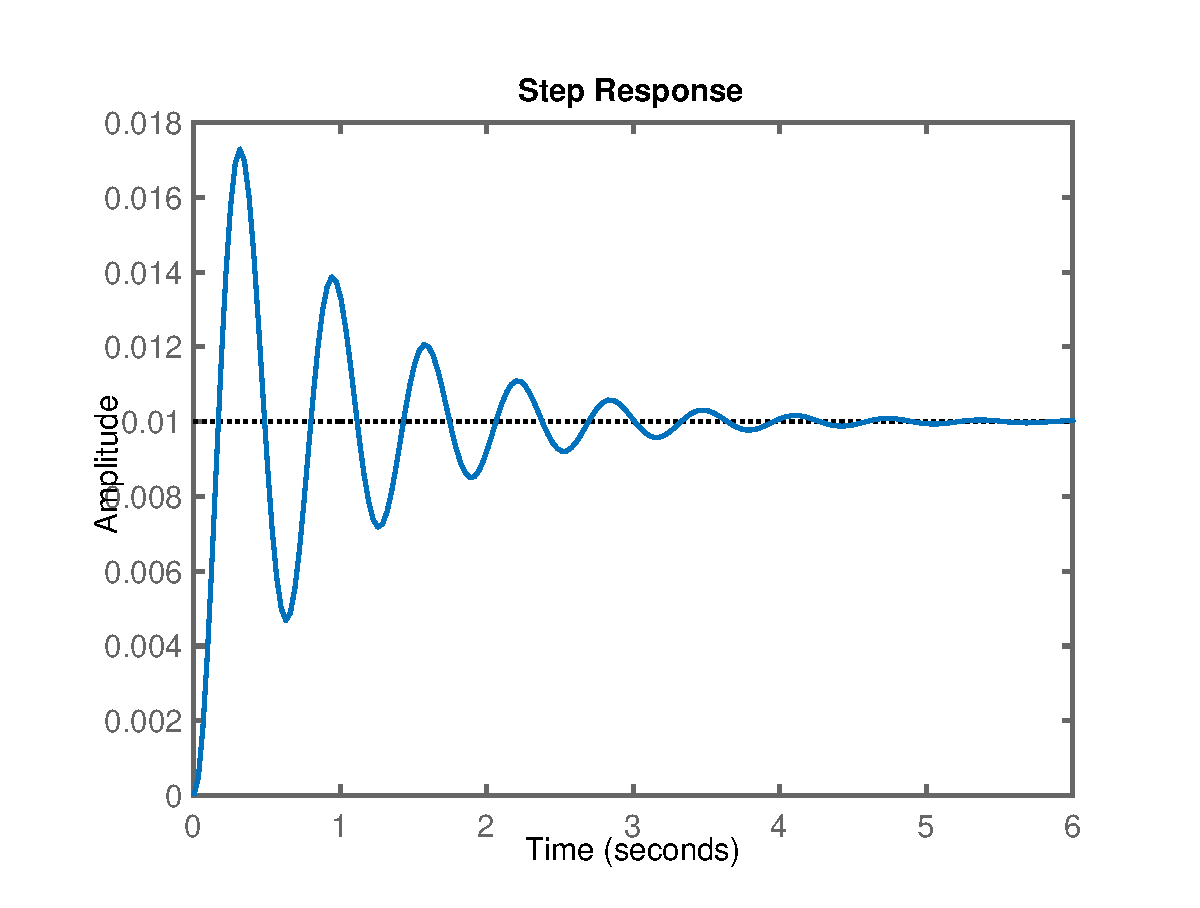
\includegraphics[width=0.5\linewidth]{Bilder/stepResponsez_02.eps}
	\caption{Step response at $\zeta = 0.2$}
	\label{Fig_stepResponsez_02}
\end{figure}
\begin{figure}[h!]
	\centering
	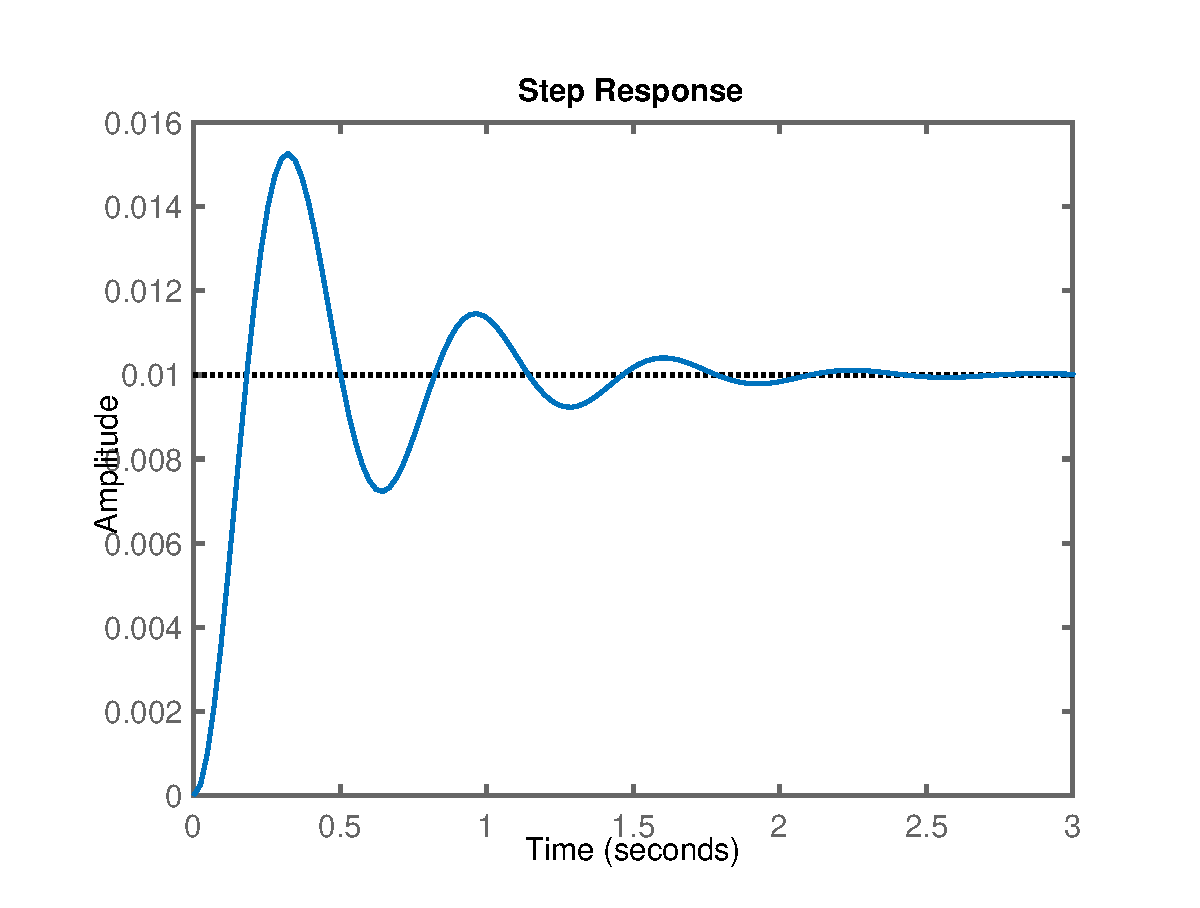
\includegraphics[width=0.5\linewidth]{Bilder/stepResponsez_04.eps}
	\caption{Step response at $\zeta = 0.4$}
	\label{Fig_stepResponsez_04}
\end{figure}
\begin{figure}[h!]
	\centering
	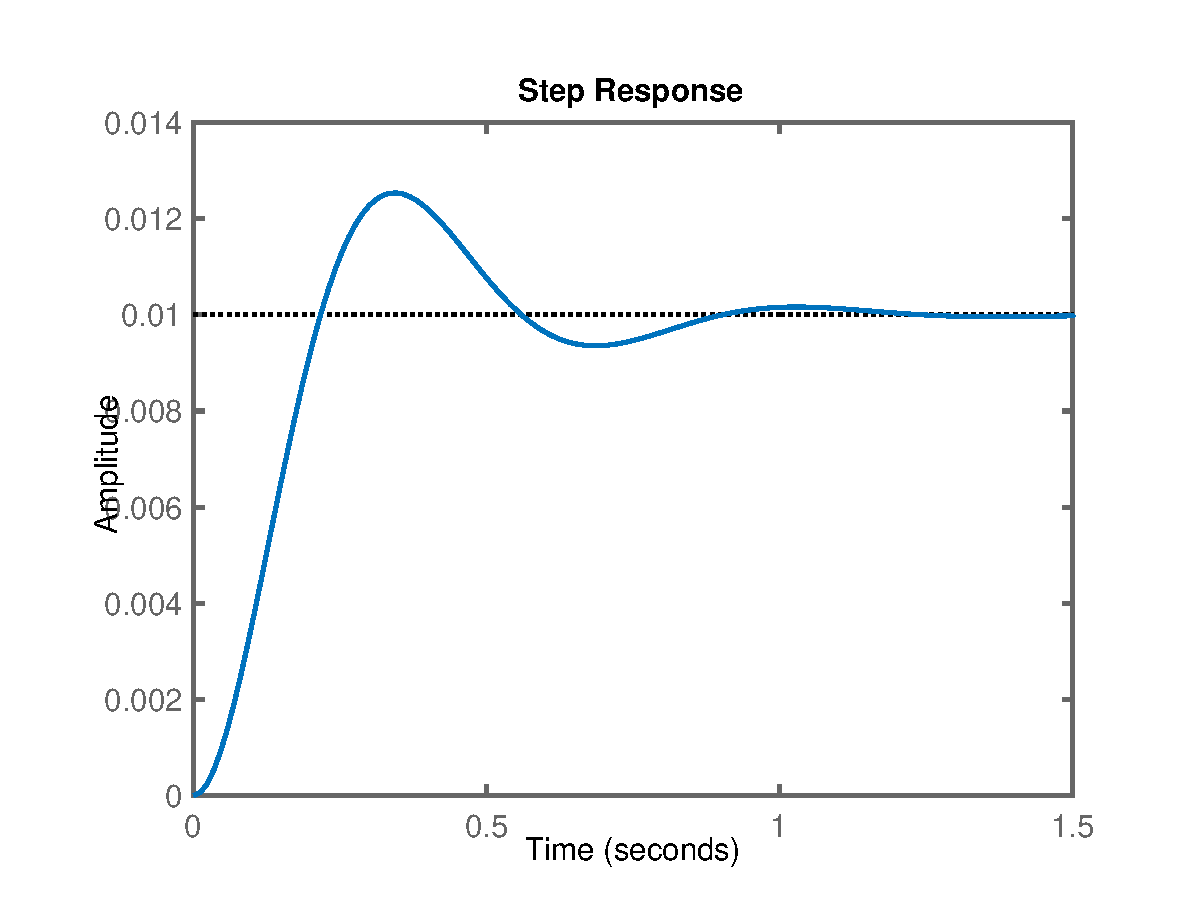
\includegraphics[width=0.5\linewidth]{Bilder/stepResponsez_08.eps}
	\caption{Step response at $\zeta = 0.8$}
	\label{Fig_stepResponsez_08}
\end{figure}
\clearpage
Going back to the example given by equation \eqref{Eq_ModelReduced_Eq}, the responses of the individual components can be plotted using Matlab as shown in figures \ref{Fig_MOR_E1_C1_step} and \ref{Fig_MOR_E1_C2_step}:
\begin{figure}[h!]
	\centering
	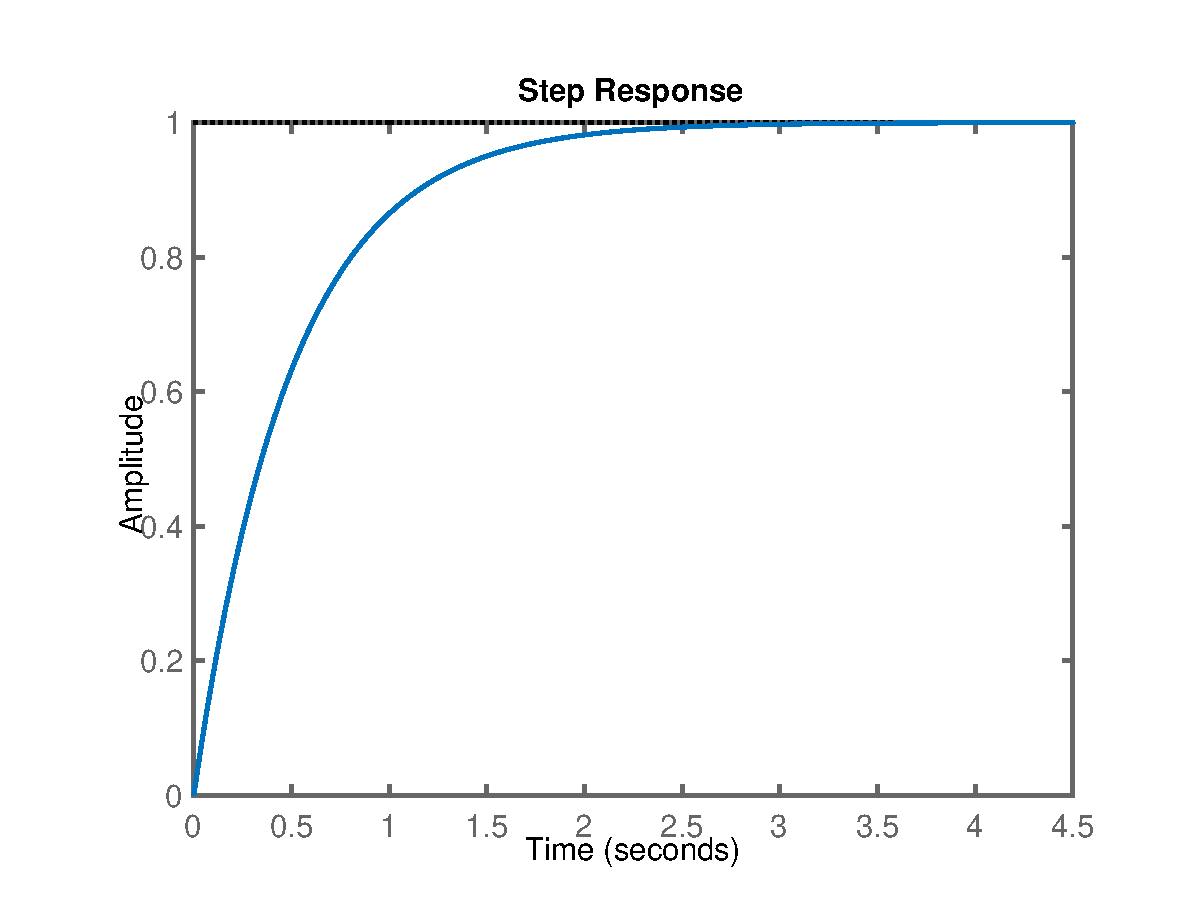
\includegraphics[width=0.7\linewidth]{Bilder/MOR_E1_C1_step.eps}
	\caption{Step response for pole at $s = -2$}
	\label{Fig_MOR_E1_C1_step}
\end{figure}
\begin{figure}[h!]
	\centering
	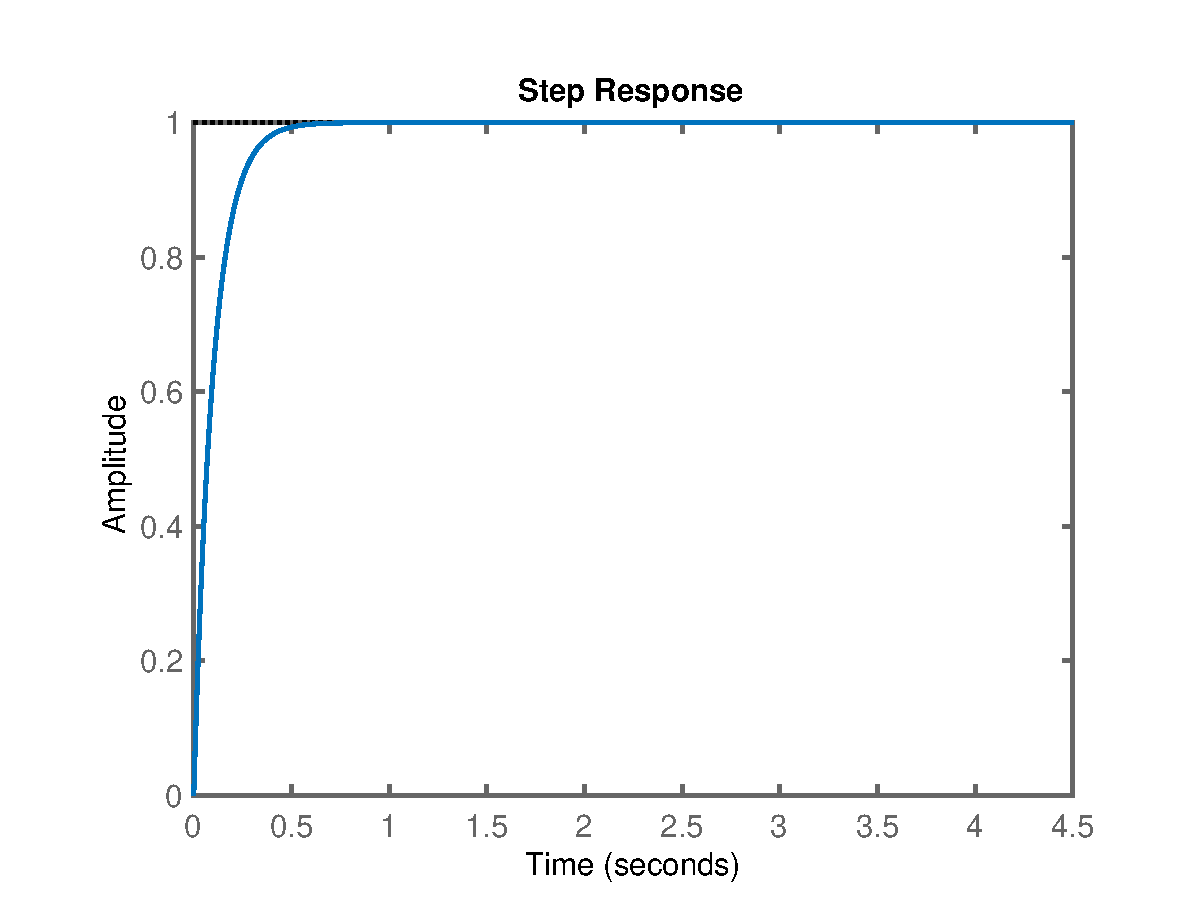
\includegraphics[width=0.7\linewidth]{Bilder/MOR_E1_C2_step.eps}
	\caption{Step response for pole at $s = -10$}
	\label{Fig_MOR_E1_C2_step}
\end{figure}
\clearpage
It can be seen clearly from figures (\ref{Fig_MOR_E1_C1_step} and \ref{Fig_MOR_E1_C2_step}) that the response of the system is much higher at higher damping ratios and this does not change the step response of the system itself. Generally since the response of component with response $e^{-2t}$ will be much slower it will dominate the overall system behavior as this makes the entire system as slow as response $e^{-2t}$ is. Consider figure \ref{Fig_MOR_E1_S_step}, which shows the response of the whole system with both the poles $s_{1,2} = \{ -2,-10 \}$
\begin{figure}[h!]
	\centering
	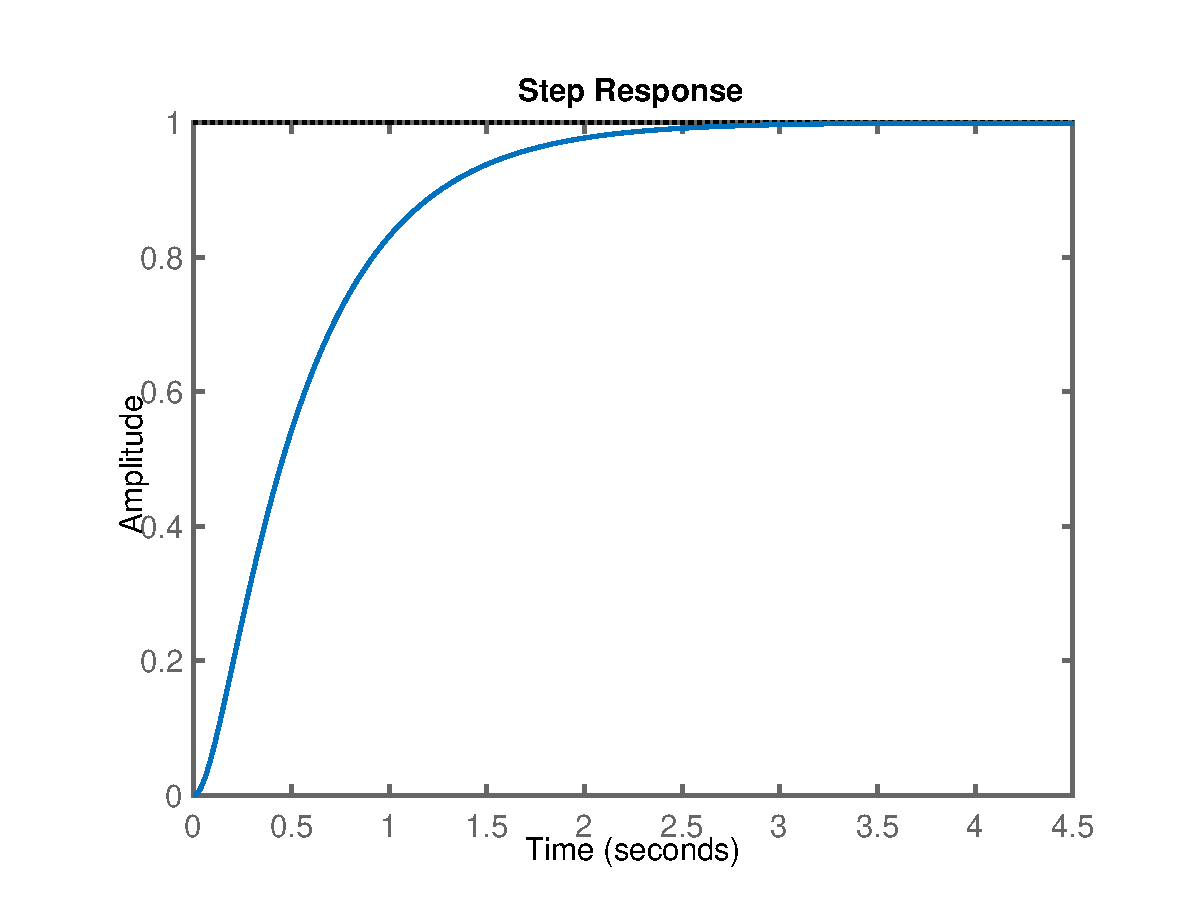
\includegraphics[width=0.7\linewidth]{Bilder/MOR_E1_S_step.eps}
	\caption{Step response for whole system with both the poles at $\{ -2,-10 \}$}
	\label{Fig_MOR_E1_S_step}
\end{figure}
It can be seen from figure \ref{Fig_MOR_E1_S_step} that the response of the system as a whole and the response of the system with only one component with pole at $s = -2$ is almost the same. Therefore, such techniques can be used to reduced the size of a higher order model by approximating the behavior to a lower order systems. 

In such a case the response of the component with response $e^{-10t}$ have almost no influence on the system, however, care has to be taken to include its steady state contribution which can be done just by using a static gain $K$ in Simulink. The size of $K$ depends on the value of the step function (DC gain from the faster component) that goes as an input to the slower component. For example if the step response (of a faster component) is of magnitude $1$, then a static gain of $K = 1$ will be given as input to the slower component. In general the gain that is needed to replace into the reduced system can be found using \textbf{\textit{final value theorem}}. Consider the system given by equation \eqref{Eq_ModelReduced_Eq}, the gain of the system can be given by:
\begin{equation}
	G(s) = \frac{20}{(s+2)(s+10)} \approx G_{Red}(s) = \frac{K}{s+2}
\end{equation}
here gain $K$ has to be set such that $G(s)$ and $G_{Red}(s)$ are both the same. $K$ or DC gain of a system is defined as \textbf{\textit{the steady-state response of the system for a DC input}} (constant input) such that:
\begin{equation}
	k_{dc} = lim_{s \rightarrow 0} s Y(s)
\end{equation}
where $$Y(s) = G(s)U(s) = \frac{20}{(s+2)(s+10)} \frac{1}{s}$$
therefore,
$$ k_{dc} = lim_{s \rightarrow 0} s \frac{20}{(s+2)(s+10)} \frac{1}{s} = lim_{s \rightarrow 0} G(s) = G(0) $$
$k_{dc}$ for the original system given by equation \eqref{Eq_ModelReduced_Eq} can be found therefore as follows:
\begin{equation}
	G(0) = \frac{20}{(0+2)(0+10)} = 1
\end{equation}
A $k_{dc} = 1$ will produce a steady-state value of $G(0) = 1$ for the system. Therefore, the DC gain of the reduced system should be $k_{dc} = 1$, such that:
\begin{equation}
	G_{Red}(s) = \frac{1}{s+2}
\end{equation}

\subsection{Effect of zeros}

\textbf{Zeros} are the values of $s$ that make the numerator of the transfer function $G(s)$ go to zero. They are the counterparts of poles. There effect on the poles can be studied using partial fraction expansion in Matlab using the command \textcolor{mygray}{[C,p] = residue(20,[1 12 20])}. 
\subsubsection{Effect 1: Contribution of each pole to the transfer function}
Consider the original system with no zeros and its partial fraction expansion:
\begin{equation}
	G(s) = \frac{20}{(s+2)(s+10)} = \frac{2.5}{s+2} - \frac{2.5}{s+10}
\end{equation}
now with zeros induced into the system the partial fraction expansion:
\begin{equation}
	G(s) = \frac{s+20}{(s+2)(s+10)} = \frac{2.25}{s+2} - \frac{1.25}{s+10}
\end{equation}
zeros effectively change the coefficients of the transfer function ie., they change the contribution of the poles on $G(s)$.
\subsubsection{Effect 2: Increases the overshoot}
Consdier the explanation given in figure \ref{Fig_EffectofZeros2}:
\clearpage
\begin{figure}[h!]
	\centering
	\includegraphics[width=\linewidth]{Bilder/Effect_of_Zeros_2}
	\caption{Zeros increase the overshoot of the system}
	\label{Fig_EffectofZeros2}
\end{figure}
As multiplication of $s$ to a transfer function is considered derivative we have a first term in the equation that the derivative of the step response. Adding the derivative part will carry the values of the derivatives to the step response which will increase the overshoot of the system as shown in figure \ref{Fig_EffectofZeros2}. Further consider figure \ref{Fig_EffectofZeros2_2}, in which it is clearly shown that zeros increase the overshoot and reduce the response time. This in-turn will induce more oscillations into the system:
\begin{figure}[h!]
	\centering
	\includegraphics[width=\linewidth]{Bilder/EffectOfZeros2_2}
	\caption{Zeros increase the overshoot of the system}
	\label{Fig_EffectofZeros2_2}
\end{figure}
\clearpage
\subsubsection{Effect 3: Non-minimum Phase Behavior}
If the zero has a \textbf{\textit{positive real root}}, then it will induce into a system a response which will initially move in the reverse direction. Such a behavior is called a non-minimal phase behavior as exhibited by a bicycle when given an impulse torque to its steering.
\subsubsection{Effect 4: Canceling poles that are near them}
\begin{figure}[h!]
	\centering
	\includegraphics[width=\linewidth]{Bilder/EffectOfZeros4}
	\caption{Zeros which are close to poles cancel them}
	\label{Fig_EffectOfZeros4}
\end{figure}
\clearpage

\subsection{Nonlinear Systems}

In most of the cases the solution to the nonlinear systems are only possible numerically. Numerical approximation of the solutions do not yield the conceptual understanding that is possible with analytical solutions. One way to have an analytical solution is to use \textbf{\textit{Model reduction techniques}} in order to simplify (approximate) the nonlinear system into a linear system in a neighborhood about an operating point. Such as the linearinzing functions that are used around an operating point in mathematics. Which defines the approximation of a nonlinear function $f(x)$ about an OP $\bar{x}$:
\begin{equation}
	\frac{df}{dx} \approx \frac{f(x) - f(\bar{x})}{\Delta x}
\end{equation}
$f(x)$ is linearized using the above relation as:
\begin{equation}
	f(x) \approx f(\bar{x}) + \frac{df}{dx} \Delta x
\end{equation}
Lienarization is possible only near the small range of neighborhood just near the OP. As the system deviates from the OP the approximation made by the lienarization deviates rapidly. A more detialed analysis on linearization is shown in chapter \ref{Ch_Linerization}.














	\chapter{System Analysis}

From the mathematical models, system analysis is performed in order to determine their behavior in time and frequency domains. Because control systems are then used on these dynamic states of the system to control their stability, steady-state error, tracking etc., among various others once the behavior in time and frequency domains are established.

\section{Time-domain analysis}

Time-domain analysis is response of the state of the dynamic system in time when given an input. The history of the response of the dynamic state due to the input is plotted as the time-response of the system. 

As dynamic systems are modeled using ODE's, their response can be determined using integration over a certain period of time either analytically or numerically. The time response of a LTI system consists of \textbf{transient response} and \textbf{steady-state response} due to an input to the system. These responses correspond to the null solution and the particular solution of the governing differential equation \cite{CTMS2019_Analysis}.

\section{Frequency domain analysis}

LTI systems have a property such that for any signaled input to the system, the output is also with the same frequency but could vary in phase and magnitude. This difference in phase and magnitude is the function of the input frequency and hence such response corresponds to the frequency response of the system \cite{CTMS2019_Analysis}.

In order to find the frequency response of the system, first the transfer function of the system is derived. Then using the complex variable $s$, the values of the plant transfer function is derived at every frequency starting from ($0$ to $\infty$). Here, $s$ is given by $s = \sigma \pm j \omega$, $\sigma$ is the real part of the root and indicates the damping in the system, $j \omega$ terms that lie on the imaginary  axis indicates the frequency of the system's oscillation. Therefore, by substituting $G(s) = G(j \omega)$ ($s = j \omega$), a frequency response of the system can be studied. If $G(s)$ is the open-loop transfer function of the system and $\omega$ is the vector of input frequencies, then the frequency response can be evaluated for every $\omega$ \cite{CTMS2019_Analysis}.

With the transfer function $G(s)$, the frequency response of the function $G(s)$ can be derived for every $s = j \omega$ and a plot of output $G(j\omega)$ versus input frequencies $\omega$ is plotted which is called \textbf{\textit{Bode Plot}}. Since $s$ is in complex plane both the magnitude and the phase of output frequencies $G(j\omega)$ can be plotted using \textbf{\textit{Bode Plot}}. As well as the position of $G(j\omega)$ in the complex plane can be studied using \textbf{\textit{Nyquist Diagrams}} \cite{CTMS2019_Analysis}.

\section{Analysis of first order systems}

A first order system hereby called PT-1 systems can be expressed in their most general form as:

\begin{equation} \label{Eq_PT1}
	\tau \dot{y}(t) + y(t) = k_{dc} u (t)
\end{equation}

Where $\tau$ and $k_{dc}$ are the parameters of the system or the constant coefficients of ODE. $k_{dc}$ is the amount of scaling of the systems output for a constant input. $\tau$ defines the amount of time required for the system to obtain $63.2 \%$ of the transient dynamics that the system undergoes. It is easier to determine the solutions of the equation \eqref{Eq_PT1} in algebraic form, \eqref{Eq_PT1} is written in the Laplace domain as:

\begin{equation} \label{Eq_PT1_TF}
	G(s) = \frac{Y(s)}{U(s)} = \frac{k_{dc}}{\tau s + 1}
\end{equation}

Again, where, $\tau$ and $k_{dc}$ are the parameters that completely define the response characteristics of a first order system and are called time constant and DC gain respectively. A time response of a PT-1 system is described using time signals such as step or impulse as inputs.

From equation \eqref{Eq_PT1_TF}, the denominator values of $s$ for which the equation goes to infinity is called the pole (values) of the system given by equation \eqref{Eq_PT1_TF}. In equation \eqref{Eq_PT1_TF}, we have only one possible value of $s$ at $s = -1/\tau$. Such a system with one pole is also defined as a first order system. Similarly a second order system will have two poles \cite[t.2.05]{RickHill_11}.

\subsection{Impulse response}

Consider a unit impulse as input to the first order system. The Laplace transform of the impulse signal is given by $L(s) = 1$. Therefore, the first order system with an impulse input is expressed as:
\begin{equation} \label{Eq_PT1_Impulse}
Y(s) = G(s)U(s) = \frac{k}{\tau s + 1} \cdot 1
\end{equation}
the inverse Laplace of the equation \eqref{Eq_PT1_Impulse} will express the solution of the equation of the differential equation \eqref{Eq_PT1} with an unit impulse input:
\begin{equation} \label{Eq:FirstOrderImpulseRespose}
y(t) = \frac{k}{\tau}e^{-\frac{t}{\tau}}
\end{equation}
The above equation is the null solution of the differential equation \eqref{Eq_PT1} given as $y = C e^{at}$ with initial condition $C = k/\tau$ and $a = -1/\tau$. From the solution \eqref{Eq:FirstOrderImpulseRespose} it can be inferred that for an unit impulse, the response of the system at time $t = \infty$ is to settle down to zero with an exponential decay. From a numerical solution generated in MATLAB, the response decays to zero as shown in figure \ref{fig:ImpulseReponseFirstOrderSystem}.
\begin{figure}[h!]
	\centering
	\includegraphics[scale=0.6]{Bilder/ImpulseReponseFirstOrderSystem.pdf}
	\caption{Impulse response of a first order system}
	\label{fig:ImpulseReponseFirstOrderSystem}
\end{figure}

\subsection{General first order responses}

A PT-1 system is first expressed in time-constant form as given below:
\begin{equation}
	\tau \frac{dy(t)}{dt} + y(t) = K u(t)
\end{equation}
where $y(t)$ and $u(t)$ are the state and inputs of the system respectively. The behavior of the system given by the above equation is described for $t > 0$ for various inputs $u(t)$ and / or initial conditions. The behavior is focused on how the output $y(t)$ changes with time constant $\tau$.

A time constant $\tau$ is defined for a more general system described by constant coefficients:
\begin{equation}
	a \frac{dy(t)}{dt} + b y(t) = c u(t)
\end{equation}
writing the above equation in time-constant form is to write the equation with coefficients of $y(t) = 1$. In such a case, the following operation is performed:
\begin{equation}
	\frac{a}{b} \frac{dy(t)}{dt} + y(t) = \frac{c}{b} u(t)
\end{equation}
therefore, the time-constant is defined by the ratio $a/b$, using the constant coefficients of PT-1 system. The ratio $a/b$ appears along with time variable $t$ in the solution of PT-1 systems and therefore serves as a factor to split and measure time, which is used to measure the system output at those factored times.

Similarly, the gain of the system is defined using the ratio $c/b$, as this appears as the coefficient of $u(t)$, it is the scaling of $y(t)$ for the given input $u(t)$. Therefore, the ratio $c/b$ is defined the gain of the system.

\subsubsection{$u(t) = 0$, non-zero initial condition}

\begin{equation}
	\tau \frac{dy}{dt} + y = 0 \implies y(t) = y(0) e^{-1/\tau}
\end{equation}

The solution shown above can be verified using LT:

\begin{equation}
	\implies \tau [s Y(s) - y(0)] + Y(s) = 0 \implies [s \tau + 1] Y(s) - \tau y(0) = 0
\end{equation}

Rearranging the above equation:
\begin{equation} \label{Eq_PT1_nonzeroICResponse}
	Y(s) = \frac{\tau y(0)}{s \tau + 1} = \frac{y(0)}{s + 1/\tau} \implies y(t) = y(0) e^{-t/\tau}
\end{equation}

These responses are characterized primarily by time-constant, which are the results derived from the solution:

\begin{enumerate}
	\item if $t = \tau$, $\implies y(t) = y(0) e^{-1} = 0.37 y(0)$
	\item if $t = 2\tau$, $\implies y(t) = y(0) e^{-2} = 0.14 y(0)$
	\item if $t = 3 \tau$, $\implies y(t) = y(0) e^{-3} = 0.05 y(0)$
	\item if $t = 4 \tau$, $\implies y(t) = y(0) e^{-4} = 0.02 y(0)$
\end{enumerate}

summary of responses:

\begin{table}[h!]
	\begin{tabular}{m{4cm} m{4cm} m{6cm}}
		\toprule
		\textbf{time} & \textbf{e} & \textbf{response} \\
		\cmidrule{1-3}
		$t = \tau$ & $e^{-1}$ & 37 $\%$ of initial condition \\
		$t = 2 \tau$ & $e^{-2}$ & 14 $\%$ of initial condition \\
		$t = 3 \tau$ & $e^{-3}$ & 5 $\%$ of initial condition \\
		$t = 4 \tau$ & $e^{-4}$ & 2 $\%$ of initial condition \\
		\bottomrule
	\end{tabular}
	\caption{Table summarizing PT-1 response for non-zero initial conditions}
\end{table}

\subsubsection{Step response}

The object is to find the solution to the differential equation $y(t)$ as given by the equation \eqref{Eq_PT1}. This system with a unit step input $u(t) = 1$ can be expressed in the Laplace domain by multipliying the input signal as:
\begin{equation} \label{Eq_PT1_step}
Y(s) = G(s) U(s) = \frac{k}{\tau s + 1}\frac{1}{s}
\end{equation}

Taking the inverse Laplace transform of equation \eqref{Eq_PT1_step}, the algebraic solution of the ODE given by equation \eqref{Eq_PT1} can be expressed as:

\begin{equation}\label{Eq_PT1_stepResponse}
y(t) = k - k e^{-t/\tau}
\end{equation}
The solution of the PT-1 system should have both null and particular solutions. The term with exponential function was initially assumed response of a homogeneous system. Therefore, the first term is the particular solution and the second term is the null solution of the ODE for PT-1 systems. In general, the terms of the null solution will impose the dynamics of the states in the system which decay after a while leaving behind the steady-state impact of the particular solution. The influence of the particular solution remains in the system as long as the input remains active without changing.

Further the stability of the system can be analyzed using \textbf{\textit{BIBO}} or using \textbf{\textit{Eigen value Analysis}}. Both the analyses lead to the same conclusion of system stability that do not blow up while operation. A BIBO stability can be performed numerically using MATLAB by choosing system parameters $\tau$ and $k_{dc}$ and a plot is generated as shown in figure \ref{fig:StepResponseFirstOrder}.
\begin{figure}[h!]
	\centering
	\includegraphics[scale=0.6]{Bilder/firstOrderSystemStepResponse.pdf}
	\caption{Step response of a first order system}
	\label{fig:StepResponseFirstOrder}
\end{figure}
Further analysis on system parameters can be made numerically such as the DC gain can be inferred from the steady-state value reached by the system. For a unit step input, the DC gain is given by the step-up value at which the output of the system's response settles down, in this case, $k = 5$ which is evident from the system value chosen to generate this plot. The time constant $\tau$ can be inferred from plot and equation \eqref{Eq_PT1_stepResponse}, for time $t = \tau$:
\begin{equation}
y(t) = k(1 - e^{-1}) = 0.632 k
\end{equation}
therefore, at one time constant $\tau$, the systems response settles down to about $63.2\%$ of the steady-state vale. Generally, a steady-state response is fixed when this value reaches $98\%$ of steady-state value, which from the plot and equation \eqref{Eq_PT1_stepResponse} can be inferred as at time $t = 4 \tau$:
\begin{equation}
y(t) = k(1 - e^{-4}) = 0.98 k
\end{equation}

Summary of PT-1 systems step response:

\begin{table}[h!]
	\centering
	\begin{tabular}{m{2cm} m{2cm} m{4cm}}
		\toprule
		\textbf{time} & \textbf{e} & \textbf{response} \\
		\cmidrule{1-3}
		$t = \tau$ & $(1 - e^{-1})$ & 63 $\%$ of steady-state response \\
		$t = 2 \tau$ & $(1 - e^{-2})$ & 84 $\%$ of steady-state response \\
		$t = 3 \tau$ & $(1 - e^{-3})$ & 95 $\%$ of steady-state response \\
		$t = 4 \tau$ & $(1 - e^{-4})$ & 98 $\%$ of steady-state response \\
		\bottomrule
	\end{tabular}
	\caption{Table summarizing step response of PT-1 system}
\end{table}

\subsubsection{step response with non-zero initial condition}

For a linear system, the response due to two different inputs can be determined using principle of superposition. Since we already now the response from step input and non-zero initial condition, they both can just be added together. Therefore, from equations \eqref{Eq_PT1_nonzeroICResponse} and \eqref{Eq_PT1_stepResponse}, we have:

\begin{equation} \label{Eq_PT1_stepAndICresponse}
	y(t) = y(0) e^{-t/\tau} + K (1 - e^{-t/\tau}) = (y(0) - K) e^{-t/\tau} + K
\end{equation}

The term $(y(0) - K) e^{-t/\tau}$ in equation \eqref{Eq_PT1_stepAndICresponse} gives the exponential decay from the IC and ss-response $K$ from step input.

The above response can also be derived using LT, by putting both LT's for IC and step-function into the equation of PT-1 system:
\begin{equation}
	[s \tau + 1] Y(s) - \tau y(0) = \frac{K}{s}
\end{equation}
then solving the above equation for $Y(s)$ and doing inverse LT, the solution can be derived.

Observations made from the solution: Consider the response given by equation \eqref{Eq_PT1_stepAndICresponse}, the following observations can be made:
\begin{enumerate}
	\item ss: depends on the gain $K$ and the input of the system. Therefore, ss = $K$
	\item Dynamics: depend on how fast the exponential goes to zero, this depends solely on the time constant $\tau$
	\item The term $(y(0) - K)$ in equation \eqref{Eq_PT1_stepAndICresponse} defines the distance from IC to the ss
\end{enumerate}

The response by changing $\tau$, let $(y(0) - K) = d$:

\begin{table}[h!]
	\centering
	\begin{tabular}{m{2cm} m{2cm} m{3cm} m{5cm}}
		\toprule
		\textbf{time} & \textbf{d}  & \textbf{y(t)} & \textbf{response} \\
		\cmidrule{1-4}
		\cmidrule{1-4}
		$t = 0$ & $ y(0) - K $ & $y = K + d = y(0)$ & At the initial state \\ \cmidrule{1-4}
		$t =  \tau$ & $ 0.37(y(0) - K) $ & $y = K + 0.37d$ & 37 $\%$ deviation from ss \\ \cmidrule{1-4}
		$t = 2 \tau$ & $ 0.14(y(0) - K) $ & $y = K + 0.14d$ & 14 $\%$ deviation from ss \\ \cmidrule{1-4}
		$t = 3 \tau$ & $ 0.05(y(0) - K) $ & $y = K + 0.05d$ & 5 $\%$ deviation from ss \\
		\bottomrule
	\end{tabular}
	\caption{Table summarizing response of PT-1 due to step input and IC}
\end{table}

From the list and the able given above, it seems that for PT-1 systems, with step input and non-zero IC, the system starts from IC and ends at ss. Where IC = $Y(0)$ and ss = $K$. 

consider an example PT-1 system:
\begin{equation}
	2 \frac{dy}{dt} + 6 y = 4 u
\end{equation}

writing in time-constant form:

\begin{equation}
	\frac{1}{3} \frac{dy}{dt} + y = \frac{2}{3} u \quad @ \quad y(0) = -1
\end{equation}

Before, generating the plot, the following observations can be made by comparing to the standard response:
\begin{itemize}
	\item $\tau = 1/3$ and $K = 2/3$
	\item at $t = 0$ response starts at $y(0) = -1$ at a distance $d = y(0) - K$ and ends at ss = $K = 2/3$ when $t > 3 \tau$
	\item for a ss of 5 $\%$, simulation time should run upto $t = 3 \tau$
\end{itemize}

\section{Stability analysis of PT-2 systems}

% For simple systems such as a rectangular cube, a clear distinction can be made easily between its equilibrium and stability states. Such that, the rotation about its principal axes is always at equilibrium, but for any perturbation, stability is guaranteed only for two among the three principal axes. However, for complex systems such as a bicycle, defining equilibrium points and stable states are more complicated. 
Once a model of a system has been established, it may be required to analyze the model in order to determine the response of the system, in this case in the time domain. In the perspective of a control design, the control system is often designed to improve the stability of the system, improve the speed of the response or the steady-state error, or prevent oscillations. Therefore, it is necessary to determine the dynamic properties of the system from the system model.
In this section, stability is defined formally for linear and non-linear systems (such as a bicycle).

\subsection{Stability in linear systems} \label{Sec_StabilityLinearSystems}

For defining the important concepts in stability analysis, a simple second order linear and homogeneous system is considered as described below:
\begin{equation} \label{Eq_SecondOrderSystem}
\Ddot{y} + B \Dot{y} + C y = 0
\end{equation}
For a special case (roots of characteristic equation lie in complex $s$ plane) such that the solution of the above ODE is given by $y = e^{st}$, the above ODE can be re-written into its characteristic algebraic form by substituting $y = e^{st}$:
\begin{equation} \label{Eq_CharacteristicEquationPT2}
s^2 + B s + C = 0
\end{equation}
the roots of the above equation are given by:
\begin{equation}
\{s_1,s_2\} = \frac{-B \pm \sqrt{B^2 - 4 C}}{2}
\end{equation}
and the null (homogeneous) solution of the equation \eqref{Eq_CharacteristicEquationPT2} can be expressed as the linear combination of roots:
\begin{equation} \label{Eq_GS_Char_PT2}
y(t) = C_1 e^{s_{1}t} + C_2 e^{s_{2}t}
\end{equation}
Alternatively, writing equation \eqref{Eq_SecondOrderSystem} in a general state equation matrix form (two first orders):
\begin{equation}
\frac{d}{dt} \begin{bmatrix}
	y \\ y^{\prime}
\end{bmatrix} = \begin{bmatrix}0 & 1 \\
-C & -B\end{bmatrix} \begin{bmatrix}y \\ y'\end{bmatrix}
\end{equation}
alternatively, the above equation can be realized in the form:
\begin{equation}
\frac{d}{dt}\vec{Z} = \begin{bmatrix} \vec{A} \end{bmatrix} \begin{bmatrix} \vec{Z} \end{bmatrix}
\end{equation}
where $\vec{Z}$ is the state matrix $[y \quad y^{\prime}]^{T}$, $\vec{A}$ is called the companion matrix (also system matrix for the dynamic states $\vec{Z}$), matrix $\vec{A}$ can be used to find the Eigen-Values of $\vec{A}$:
\begin{equation}
\{\lambda_1,\lambda_2\} = \frac{-B \pm \sqrt{B^2 - 4 C}}{2}
\end{equation}
and the null solution of the second order differential equation:
\begin{equation}
y(t) = C_1 e^{\lambda_{1}t} + C_2 e^{\lambda_{2}t}
\end{equation}
Both the null solutions predicted by the roots $\{s_1,s_2\}$ and Eigen-Values $\{\lambda_1,\lambda_2\}$ give the solution of the differential equation \eqref{Eq_SecondOrderSystem}, however, with Eigen-values it is much easier to reach at the null solution. %as the problem now is transformed from differential calculus to linear algebra.
From the roots $\{s_1,s_2\}$ or the Eigen-Values $\{\lambda_1,\lambda_2\}$, following cases can be drawn about the stability of the second order system:

\begin{table*}[h!] \centering
	\begin{tabular}{ccc}
		\toprule
		Cases & Condition & Eigen-Values \\ \hline 
		\\
		Over-damped & $(B^2 > 4 C)$ & Negative distinct Roots \\
		Critically damped & $(B^2 = 4 C)$ & Negative repeated roots \\
		Under-damped & $(B^2 < 4 C)$ & Complex conjugate roots \\
		Undamped & $B = 0$ & Imaginary Roots \\
		\bottomrule
	\end{tabular}
	\label{Tab_PT2_Char_Roots}
\end{table*}

Since the characteristic equation \eqref{Eq_CharacteristicEquationPT2} is quadratic in nature, the roots will be of complex in nature. With complex roots it can be said that the imaginary part will indicate the frequency of systems oscillations and the real part will indicate the damping (or growth based on parameter $B$) of the system. In case of undamped system, even the BIBO stability can not be said to be achieved completely as the system will be oscillating with an undamped magnitude (high risk of resonance). Therefore, the BIBO and the asymptotic stability of the system can only be defined in the cases where there is a damping \cite{RickHill_11}.

In terms of BIBO stability the stability of the PT-2 system can be roughly described using the values of the real part and can be described as follows:
\begin{itemize}
	\item Pure oscillations: Real part of poles is zero.
	\item Exponential decay (BIBO stability): Real part are negative.
	\item Exponential growth (unstable): If at-least one of the Real part is positive.
\end{itemize}

\textbf{Asymptotic stability}: The PT-2 system is considered to be asymptotically stable if and only if, the state $x \rightarrow 0$ as $t \rightarrow \infty$ \cite[t.8.45]{RickHill_11}.

\textbf{BIBO stability}: A system is said to be BIBO stable if for any bounded inputs the system outputs remain bounded ie., the system output does not blow up.

For linear systems, using these two stability criterion the stability of PT-2 system can be established.

\subsection{Stability Analysis in Non-linear systems} \label{Sec:StabilityNonLinearSystems}

With linear systems, if the system is already in the stable condition, then regardless of the initial conditions, the system will get back to its stable position. However, a non-linear system is stable only if the perturbations lie within a certain range of neighborhood. Lets consider a non-linear autonomous system (time-invariant system) expressed as a first order system dependent on velocity:
\begin{equation}
\Dot{x} = f(x)
\end{equation}
The equilibrium states can be defined for a non-liner system if it satisfies the condition:
\begin{equation}
\Dot{x} = f(x_{e}) = 0 \quad \forall t > t_0
\end{equation}
where $x_e$ is the point at which the function $f(x) = 0$ and $x_e = constant$. The neighborhood is defined as: Given perturbation $\delta > 0$, a state vector $x(t)$ is said to be in the neighborhood $B_b(x_r(t))$ of the state $x_r(t)$ if:
\begin{equation}
\norm{x(t) - x_r(t)} < \delta
\end{equation}
then,
\begin{equation}
x(t) \quad \in \quad B_{\delta}(x_r(t))
\end{equation}

\begin{figure}[h!]
	\centering
	\includegraphics[scale=0.5]{Bilder/Neighborhood.eps}
	\caption{Neighborhood of a non-linear system stability}
	\label{fig:Neighborhood}
\end{figure}

\textbf{\textit{Lagrange stability}} is defined as: the state $x(t)$ is said to be Lagrange stable (or bounded) relative to $x_r(t)$ if there exists a $\delta > 0$ such that:
\begin{equation}
x(t) \quad \in \quad B_{\delta}(x_r(t)) \quad \forall t > t_0
\end{equation}

\begin{figure}[h!]
	\centering
	\includegraphics[scale=0.5]{Bilder/LagrangeStability.eps}
	\caption{Lagrange Stability}
	\label{fig:LagrangeStability}
\end{figure}

\textbf{\textit{Lyaponov stability}} of non-linear system is defined as: the state $x(t)$ is said to be Lyaponov stable relative to $x_r(t)$ if for each $\epsilon > 0$ there exists a $\delta(\epsilon)>0$ such that:
\begin{align}
x(t_0) \quad &\in \quad B_{\delta}(x_r(t_0)) \\
x(t) \quad &\in \quad B_{\epsilon}(x_r(t)) \quad \forall t > t_0
\end{align}
Unlike Lagrange stability, in Lyaponov stability lets to define another neighborhood $B_{\epsilon}(x_r(t))$ such that perturbations in the previous neighborhood $B_{\delta}(x_r(t_0))$ would lead to $B_{\epsilon}(x_r(t))$, hence, unlike Lagrange stability which does not depend on the initial conditions (but on the physics of the problem) Lyaponov stability narrows down the initial states that could lead to stability in the motion in a later state. Also, unlike in the linear systems, the non-linear systems would lead to convergence just because the system is in the stable condition. The boundary $B_{\epsilon}(x_r(t))$ could be very close to $B_{\delta}(x_r(t_0))$ and the system would be stable in the $\epsilon$. For numerical simulation, it is required that the simulations are run for long enough time to prove that the stability remains within the conditions described by the Lyaponov conditions.

\begin{figure}[h!]
	\centering
	\includegraphics[scale=0.5]{Bilder/LyaponovStability.eps}
	\caption{Lyaponov Stability}
	\label{fig:LyaponovStability}
\end{figure}

Once Lyaponov stability has been defined, an \textbf{\textit{Asymptotic stability}} can be extended and defined as: the state $x(t)$ is asymptotically stable relative to $x_r(t)$ if $x(t)$ is Lyaponov stable and there exists a $\delta > 0$ such that:
\begin{align}
x_0(t) \quad &\in \quad B_{\delta}(x_r(t_0)) \quad \text{then,}\\
\lim_{t\to\infty} x(t) \quad &= \quad x_r(t)
\end{align}
\begin{figure}[h!]
	\centering
	\includegraphics[scale=0.5]{Bilder/AsymptoticStability.eps}
	\caption{Asymptotic stability}
	\label{fig:AsymptoticStability}
\end{figure}
Therefore, in case of asymptotic stability, the boundary due to $\epsilon$ goes to zero and the boundary $B_{\epsilon}(x_r(t))$ does not exists anymore, so now the motion $x(t)$ converges to the reference $x_r(t)$. This is an ideal condition to converge to from controls perspective. Certain dynamic systems have shown to converge to this stability point in their natural modes of operation. A bicycle is one such example where under a certain range of velocities the weave motion of the bicycle converges to asymptotic stability by damping (not physically damping like in friction) the weave motion towards a zero lean and steering rates. 

\subsection{Solving / Analysing PT-2 using Laplace transform} \label{Sec_Solving_PT2_Laplace}

Laplace transform of the PT-2 system can be expressed as:
\begin{equation}\label{Eq_Laplace_PT2}
G(s) = \frac{Y(s)}{U(s)} = \frac{\omega_{n}^{2}}{s^{2} + 2 \zeta \omega_{n} s + \omega_{n}^{2}}
\end{equation}
the poles of the denominator in equation \eqref{Eq_Laplace_PT2} can be found:
\begin{equation*}
s_{1,2} = \frac{-2 \zeta \omega_{n} \pm \sqrt{4 \zeta^{2} \omega_{n}^2 - 4 \omega_{n}^2}}{2} = -\zeta \omega_{n} \pm \omega_{n} \sqrt{\zeta^2 - 1} = -\zeta \omega_{n} \pm j \omega_{n} \sqrt{1 - \zeta^2}
\end{equation*}

with poles $s_{1,2} = -\zeta \omega_{n} \pm j \omega_{n} \sqrt{1 - \zeta^2}$, the stability analysis of the system can be made based on the numerical values of the roots. Only $\zeta$ is a variable and $\omega_{n}$ is a constant also $\zeta$ can be controlled as a variable as the system frequency $\omega$ varies. Therefore, $\zeta$ now becomes the fundamental variable for the behavioral changes in the motion as follows:
\begin{table}[h!]
	\centering
	\begin{tabular}{m{4em} m{8em} m{8em}}
		\toprule
		$\zeta = 0$ & poles are Im  & undamped \\
		$\zeta < 1$ & poles are complex & under-damped \\
		$\zeta = 1$ & repeated real poles & critically damped \\
		$\zeta > 1$ & distinct real poles & over damped \\ \bottomrule
	\end{tabular}
\end{table}
\begin{figure}[h!]
	\centering
	\includegraphics[width=\linewidth]{Bilder/Poles_PT2_system}
	\caption{Poles in the PT2 system}
\end{figure}

\subsubsection{Determining the system behavior} \label{Sec_PT2_system_properties}

Various system behaviours can be determined using the resuts from the previous analysis and they are important which define the PT-2 systems acording to their behavior. Using an underdamped system response various system behaviors can be defined as with underdamped systems all the system behaviorial characteristics are clearly visible. Using Laplace transforms with a step function the solution of PT-2 system can be found using inverse Laplace as shown in the red box in figure \ref{Fig_Sol_PT2_StepInput_Laplace}.
\begin{figure}[h!]
	\centering
	\includegraphics[width=\linewidth]{Bilder/Sol_PT2}
	\caption{Solution to PT-2 system with step input using Laplace transform}
	\label{Fig_Sol_PT2_StepInput_Laplace}
\end{figure}
Several important properties highlighted by the solution obtained in figure \ref{Fig_Sol_PT2_StepInput_Laplace} can be seen visually as shown in figure \ref{Fig_Prop_PT2_Laplace}.
\clearpage
\begin{figure}[h!]
	\centering
	\includegraphics[width=\linewidth]{Bilder/Prop_PT2}
	\caption{Important behvarial propertial seen in PT-2 systems}
	\label{Fig_Prop_PT2_Laplace}
\end{figure}
These important properties can be listed as follows:
\begin{enumerate}
	\item Delay time
	\item Rise time
	\item Settling time
	\item Peak time
	\item Maximum Overshoot
\end{enumerate}
the definitions and analytical deduction of the properties are given in figures (\ref{Fig_Delay_and_Rise_PT2_Laplace}, \ref{Settling_time_PT2}, \ref{Peak_time_PT2} and \ref{Max_overshoot_PT2}).
\begin{figure}[h!]
	\centering
	\includegraphics[width=\linewidth]{Bilder/Delay_and_Rise_time_PT2}
	\caption{Delay and Rise times seen in PT-2 systems}
	\label{Fig_Delay_and_Rise_PT2_Laplace}	
\end{figure}
\clearpage
\begin{figure}[h!]
	\centering
	\includegraphics[width=\linewidth]{Bilder/Settling_time}
	\caption{Settling time seen in PT-2 systems}
	\label{Settling_time_PT2}	
\end{figure}
Settling time is approximated by roughly determining the time required to settle down the state dynamics by 2\% at the steady state. The sinusoid inside the brackets will produce oscillations all the time unless they are completely damped out as $t \rightarrow \infty$. However by controlling the exponential value to reach $2\%$, the output from the sinosoids can be be controlled within $2\%$. Therefore, from the analogy that $e^{-4} \approx 0.02$, the settling time $t_s$ is approximated to $4 / \sigma$.
\begin{figure}[h!]
	\centering
	\includegraphics[width=\linewidth]{Bilder/Peak_time_PT2}
	\caption{Peak time seen in PT-2 systems}
	\label{Peak_time_PT2}	
\end{figure}
\begin{figure}[h!]
	\centering
	\includegraphics[width=\linewidth]{Bilder/Max_overshoot_PT2}
	\caption{Maximun overshoot seen in PT-2 systems}
	\label{Max_overshoot_PT2}	
\end{figure}

\clearpage

\subsection{Poles determine the system behavior} \label{Sec_PolesDetSysBehv}

Consider figure \ref{Fig_PolesSystemBehavior}, from the poles placed in the complex plane the following details can be extracted. The distance of the poles on the real axis is given by the real part of the roots and the distance of the poles on the imaginary axis is given by the Im part of the poles. The radius of the poles from the origin is defined by the natural frequency of the system $\omega_{n}$ and the angle between pole radius $\omega_{n}$ and real axis is given by $\beta$.
\begin{figure}[h!]
	\centering
	\includegraphics[width=\linewidth]{Bilder/PolesDetermineSysBehavior}
	\caption{Poles determine the system behavior}
	\label{Fig_PolesSystemBehavior}
\end{figure}

From the relationship $cos{\beta} = \zeta$ it can be said that the angle $\beta$ determines the damping in the system such as when $cos{\beta} = \pi/2$ then damping is zero and the system oscillates freely. When $cos{\beta} = 0$, the poles lie exactly on the real axis and also lie on one another (repeated poles), making the system critically damp. Therefore, as the angle $cos{\beta}$ increases towards $\pi/2$, the damping in the system decreases and vice-versa.

\subsection{Solving / Analysis PT-2 using characteristic polynomial}

The general form of PT-2 using a characteristic polynomial is given by equation \eqref{Eq_CharacteristicEquationPT2} (the coefficients in various forms may vary but they don't change the solution or the behavior as they are constants and treated differently in different approaches). From the table \ref{Tab_PT2_Char_Roots}, the roots of the polynomial can be used to define the systems damping and therefore its behavior. For the first analysis, consider case (1) in the table \ref{Tab_PT2_Char_Roots} for roots $B^{2} > 4C$ leading to definite negative roots which overcome the oscillations from the Im roots and therefore make the system over damped.

With the roots of the characteristic equation \eqref{Eq_CharacteristicEquationPT2} given by $\{s_1, s_2\}$, the general solution of equation \eqref{Eq_CharacteristicEquationPT2} can be expressed as the linear sum of the solution of each roots as given by:
\begin{equation}
	y(t) = A e^{s_{1}t} + B e^{s_{2}t}
\end{equation}
where $A$ and $B$ are constants which are determined using initial conditions which is same as equation \eqref{Eq_GS_Char_PT2} just with different coefficients. Now equation \eqref{Eq_GS_Char_PT2} gives the general solution for a homogeneous PT-2 given by \eqref{Eq_CharacteristicEquationPT2}. For the sake of analysis, lets use a step function and perform a time-domain analysis of PT-2 systems. Now equation \eqref{Eq_SecondOrderSystem} can be written for a step input as:
\begin{equation} \label{Eq_PT2_stepInput}
	a \ddot{y} + b \dot{y} + c = 1
\end{equation}
the 1 on RHS signifies the external step input, with initial conditions $x(0) = \dot{x}(0) = 0$. Therefore now the general solution to equation \eqref{Eq_PT2_stepInput} is given by:
\begin{equation} \label{Eq_GS_PT2_stepInput}
	y(t) = A e^{s_{1}t} + B e^{s_{2}t} + \frac{1}{c}
\end{equation}
$A$ and $B$ can be solved using initial condition's using $y(t)$ and $\dot{y}(t)$ leading to:
\begin{align*}
	\left(\frac{s_2}{s_1} - 1 \right) B &= \frac{1}{c} \\
	A &= \frac{-s_2}{s_1} B
\end{align*}
therefore, equation \eqref{Eq_GS_PT2_stepInput} becomes:
\begin{equation}
	y = \frac{1}{c} \left[ 1 + \left( \frac{1}{s_1 + s_2} (s_1 e^{s_{2}t} - s_2 e^{s_{1}t}) \right) \right]
\end{equation}
$c$ can be determined at the steady-state such that at steady state $\ddot{y} = \dot{y} = 0$ which leads to $c = 1$ in equation \eqref{Eq_SecondOrderSystem}.

\subsection{Numerical solution for PT-2 systems using Matlab}

For linear systems, Matlab has many inbuilt functions that can be used directly to determine the various system properties given in section \ref{Sec_PT2_system_properties}. It is only necessary to remember these properties rather than be able to solve them analytically. Control system toolbox in Matlab can be used to conveniently determine all these properties on a computer rather by solving with pen and paper as well plot results to see these properties graphically for understanding.

Using the command \textbf{\textit{linearSystemAnalyzer('step',G)}}, a figure shows in Matlab all the properties of a linear PT-2 system which are evaluated numerically.

	\chapter{Introduction to Control}

In chapters System modeling and Analysis, systems were modeled and analyzed by their time-response behavior by using a step function. Once the system behavior is observed and its properties defined as described in section \ref{Sec_PT2_system_properties}, sometimes most of the system properties such as its response may not be the desired response that one is looking for. In such cases system behavioral properties can be modified using a \textbf{\textit{control}}.

\section{Control Architectures}

\subsection{Open-loop control / Feedforward control} \label{Sec_OL_ControlArchitecture}

Simple to design in controls perspective given predefined disturbances and plant dynamics. The open loop control architecture can be visualized using block diagrams as shown in figure \ref{fig_OpenLoopControl}.
\begin{figure}[h!]
	\centering
	\includegraphics[width=0.8\linewidth]{Bilder/OpenLoopControl}
	\caption{Open Loop Control Architecture}
	\label{fig_OpenLoopControl}
\end{figure}
\clearpage
The control in the open loop architecture works as an inverted plant which can be explained as follows. The idea is to have output signal $Y(s)$ follow the reference signal $R(s)$. If the disturbance signal $D(s)$ is ignored the output signal of the entire system can be expressed as $Y(s) = P(s)C(s)R(s)$. If the condition that $Y(s) = R(s)$ to be met, it follows that $P(s)C(s) = 1$. If $P(s)C(s) = 1$ should be met then it follows that $C(s) := 1/P(s)$. Therefore, the control in an open-loop is just the plant inverted. This is the most simple form of control that can be applied just by inverting the plant dynamics and it requires no additional components such as sensors.

Obviously this type of design is not robust mainly because of the follows two reasons:
\begin{itemize}
	\item Model errors: It is not sometimes possible to capture the dynamics of the system perfectly or the parameters of the system would change over time or there could also be some after market changed in the system that were not previously accounted for.
	\item The disturbances to the system cannot be pre-defined accurately as this is some unknown quantity that is being influenced from the environment.
\end{itemize}
Open-loop architecture is used in the most simplified cases where the control will not be affected from external disturbances such as in washing machines where the system is isolated from the environment and the control can do its work without any external influences. Or they are also used in conjunction with feedback in complex systems as the tracking error with open-loop can be essentially eliminated to zero.

\subsection{Closed Loop Architecture / Feedback control} \label{Sec_ClosedLoopArchitecture}

Feedback control architecture will make the control system robust by using a feedback of the system outputs via a sensor. Feedback controller uses the differences between output and the reference signal to calculate the control action required to reduce the tracking error. In short feedback control works by providing a control action with respect to the error signal generated. The architecture is shown in figure \ref{fig_ClosedLoopControl}
\begin{figure}[h!]
	\centering
	\includegraphics[width=0.8\linewidth]{Bilder/ClosedLoopControl}
	\caption{Closed Loop Control Architecture}
	\label{fig_ClosedLoopControl}
\end{figure}
\newpage
One drawback of closed loop control is that it could induce instability into the system. The controller and the plant themselves my be stable on their own with negative real roots in the transfer function. But when the loop is closed the system on its whole could become unstable.

\textbf{Use of feedback: Dynamics of individual components need not be modeled}

With a feedback unlike in open-loop control, the knowledge of the individual components of the system need not be known. For example consider system shown in figure \ref{fig_Feedback_Use1}, where the position of a spindle is controlled using an electric motor.
\begin{figure}[h!]
	\centering
	\includegraphics[width=0.8\linewidth]{Bilder/Feedback_Use1}
	\caption{Use of Feedback}
	\label{fig_Feedback_Use1}
\end{figure}
It can be seen from figure \ref{fig_Feedback_Use1}, that the control on position is implemented only using the voltage to the motor as input. The individual dynamics of components such as functioning of the motor and the load inertia themselves may not even be modeled into the system. For example using a step input the response of the system can be modeled as a whole (either as PT-1 or PT-2 or the combination of both).

\textbf{Use of feedback: Make system robust and disturbance rejection}

Making a system robust is in essence successfully reject disturbance and overshadow the plant and sensor properties while controlling. For example consider a complex system as shown in figure \ref{fig_Feedback_Use2}, in order to determine what parameters the output of this system depends, a output can be determined using transfer function of the whole system:
 \begin{figure}[h!]
 	\centering
 	\includegraphics[width=0.8\linewidth]{Bilder/Feedback_Use2}
 	\caption{Use of Feedback: Making the system robust}
 	\label{fig_Feedback_Use2}
 \end{figure}

\begin{equation}
	Y(s) = F \frac{GK}{1 + GKH} r + G_d \frac{G}{1 + GKH} d_e + \frac{GKH}{1 + GKH}n
\end{equation}
when the controller gain $K$ is made significantly large, in the above equation, the following terms would take the following values:
\begin{align*}
	\frac{GK}{1 + GKH} &= 1 \\
	\frac{G}{1 + GKH} &= 0 \\
	\frac{GKH}{1 + GKH} &= 1
\end{align*}
therefore, the system output equation reduces to:
\begin{equation} \label{Eq_FeedbackUse2_Eq}
	Y(s) = F r + n
\end{equation}
From equation \eqref{Eq_FeedbackUse2_Eq}, it can be seen that when $K$ is significantly large, the response of the system becomes mostly dependent on reference TF $F$ with signal $r$ and noise signal $n$. The dynamics of plant $G$, sensor $H$ is removed from the equation, therefore the change in the dynamics of the plant or the senor will have almost no impact on the control system itself. Further the equation \eqref{Eq_FeedbackUse2_Eq} does not contain the term of disturbance $G_e$, therefore, the effect of disturbance is also rejected by the use of feedback.

\section{Block diagram reduction} \label{Sec_BlockDiagReduction}

Basically the stability or the response of the system depends on the poles. In order to be able to determine the poles of the entire system each individual blocks of the system should be reduced to form a single component system so that the transfer function and in-turn the poles of the system can be calculated easily.
\begin{figure}[h!]
	\centering
	\includegraphics[width=0.8\linewidth]{Bilder/BDR_1}
	\caption{Block diagram reduction: Algebraic}
	\label{fig_BDR_1}
\end{figure}
\begin{figure}[h!]
	\centering
	\includegraphics[width=0.8\linewidth]{Bilder/BDR_2}
	\caption{Block diagram reduction: Memorizing rules}
	\label{fig_BDR_2}
\end{figure}
\begin{figure}[h!]
	\centering
	\includegraphics[width=0.8\linewidth]{Bilder/BDR_3}
	\caption{Block diagram reduction: Series and Parallel}
	\label{fig_BDR_3}
\end{figure}
\clearpage

\section{Linearity and Principle of Superposition}

For linear systems with multiple inputs, the effect of each of the individual signals into the system can be studied separately by ignoring all other signals into the system block diagram as in linear systems the response of the system for all the inputs can later be added up to determine the overall system response as explained in a very clear detail graphically in \cite[t.41.19]{RickHill_13}.

\section{Cruise control example and drawbacks of proportional regulator}

As described in section \ref{Sec_ClosedLoopArchitecture} of closed loop architecture, once the error has been determined the controller can use this error to provide some control signal to the actuator which in-turn will reduce the tracking error. Once the error has been determined there are many ways in control theory to use this error to determine the control signal in-turn. One easiest way to calculate the control signal is by using a proportional gain regulator.

\subsection{Open-loop system model}

The cruise control system controls the traction force $F$ (or traction force is the control signal) and the tracking is required on the output velocity of the vehicle $v$. A longitudinal dynamic model of a vehicle is choose for simplicity and also noting that for a cruise control which controls only the output velocity $v$ of the vehicle, such simplified longitudinal model is sufficient. From longitudinal model it can be said that the accelerating force that is required to maintain desired $v$ can be found from Newtons second law as:
\begin{equation} \label{Eq_LongVehicleModel}
	F - F_{res} = m \dot{v}
\end{equation}
where $F$ is control signal generated to accelerate the vehicle, $F_{res}$ are the longitudinal resistance the vehicle experiences due to air drag, rolling resistance and gradient resistance, $\dot{v}$ is the vehicle acceleration and $m$ is the system parameter. Additionally, $F_{res}$ can be approximated as function of $v$ and a linear function as:
\begin{equation}
	F_{res} = b v
\end{equation}
where $b$ is a system parameter that influences $F_{res}$. Equation \ref{Eq_LongVehicleModel} becomes:
\begin{align}
	F - b v &= m \dot{v} \\
	m \dot{v} + b v = F \label{Eq_ODE_LongVehicleModel}
\end{align}
Equation \eqref{Eq_ODE_LongVehicleModel} forms the first order ODE of the longitudinal vehicle model. And the Laplace transform of equation \eqref{Eq_ODE_LongVehicleModel} is:
\begin{equation} \label{Eq_LP_ODE_VehicleModel}
	m s V(s) + b V(s) = F(s)
\end{equation}
writing in terms of transfer function:
\begin{equation} \label{Eq_TF_ODE_VehicleModel}
	\frac{V(s)}{F(s)} = \frac{1}{ms + b}
\end{equation}
writing equation \eqref{Eq_TF_ODE_VehicleModel} in canonical form:
\begin{equation}
	\frac{V(s)}{F(s)} = \frac{1/b}{\frac{m}{b}s + 1}
\end{equation}
where $k_{dc} = 1/b$ which will also give the steady-state response and $\tau = m/b$ which gives the settling time (or time constant) of the plant and $\frac{V(s)}{F(s)}$ gives the transfer function of the plant. 

\subsection{Closed Loop Model}

Now a controller with proportional gain $K$ is added in series to the plant which actuates with reference signal $R(s)$ and $V(s)$ will be the output of the entire system as shown in figure \ref{Fig_CruiseControlPRegulator}. Since this is closed loop transfer function, the block diagram reduction is shown in section \ref{Sec_BlockDiagReduction} in figure \ref{fig_BDR_2} will lead to the following system TF:
\begin{equation}
	\frac{V(s)}{R(s)} = \frac{\frac{K}{ms+b}}{1 + \frac{K}{ms+b}}
\end{equation}
simplifying the above equation leads to:
\begin{equation}
	\frac{V(s)}{R(s)} = \frac{\frac{K}{b + K}}{\frac{m}{b + K}s + 1}
\end{equation}
\begin{figure}[h!]
	\centering
	\includegraphics[width=\textwidth]{Bilder/Cruise_Control_P_Regulator.pdf}
	\caption{Block diagram of Cruise controller with P-type regulator}
	\label{Fig_CruiseControlPRegulator}
\end{figure}
therefore, $k_{dc}$ and time constant of the system are $\frac{K}{b + K}$ and $\frac{m}{b + K}$ respectively. If $K$ is chosen sufficiently larger then it will dominate the terms $k_{dc}$ and $\tau$ such that $k_{dc} \rightarrow 1$ and $\tau \rightarrow 0$ which is the most ideal case for the controller leading to perfect tracking with fast response. Additionally, the pole is at $s = \frac{-(b + K)}{m}$ and as $K$ increases the roots become more negative and this will lead to much faster response times of the controller. With no external disturbances and noise in the system the control does the tracking perfectly as shown in figure \ref{Fig_P_Regulator_Tracking}. However, a feedback loop also induces proportional noises into the system proportional to $K$ which has to be studied separately.
\begin{figure}[h!]
	\centering
	\includegraphics[width=0.6\linewidth]{Bilder/P_Reg_Tracking.eps}
	\caption{Tracking achieved by Hight Propotional controller gain}
	\label{Fig_P_Regulator_Tracking}
\end{figure}

\subsection{Effects of Noise with Proportional Regulator} \label{Sec_NoiseInClosedloopArchitecture}

With noise as the input signal (ignoring $R(s)$) the closed loop TF of the system is expressed as:
\begin{equation} \label{Eq_CL_Noise}
	\frac{V(s)}{N(s)} = \frac{-\frac{K}{ms + b}}{1 + \frac{K}{ms + b}} = \frac{-K}{ms + b + K}
\end{equation}

From equation \ref{Eq_CL_Noise}m it can be seen that when $K$ is made sufficiently large, the TF will increase towards a value of $-1$. A TF of $-1$ will make the system output $V(s)$ react to noise in the opposite to the desired value and it amplifies as $K$ increases. Therefore, a larger $K$ will amplify the effect of noises into the system and such cases the system will fail to track as shown in figure \ref{Fig_P_Regulator_Tracking_Noise}.
\begin{figure}[h!]
	\centering
	\includegraphics[width=0.6\linewidth]{Bilder/P_Reg_with_Noise.eps}
	\caption{Tracking failed by high Proportional controller gain with noise}
	\label{Fig_P_Regulator_Tracking_Noise}
\end{figure}

Additionally, there is also something called actuator saturation that comes from larger $K$ ie., limit of engine dynamics, friction between tire-road interface among others which would lead to higher fuel consumption among others. Additionally a larger $K$ will induce system oscillations. Therefore, it is necessary to avoid larger $K$ due to noise disturbance amplifications, actuator saturation and system oscillations (due to overshoot).










	\chapter{Eigen Value Analysis}

Eigenvalues tells about how the given system matrix $\vec{A}$ will respond or evolve in the particular direction of Eigenvectors. Consider a system matrix given by
\begin{equation}
	\vec{A} = \begin{bmatrix}
	1 & 0 \\ 0 & -1
	\end{bmatrix}
\end{equation}
the Eigenvalues and the Eigenvectors of the system are given by
\begin{align*}
	\lambda_{1} & = 1 \\
	\lambda_{2} &= -1 \\
	v_1 & =	\begin{bmatrix}
	1 \\ 0
	\end{bmatrix} \\
	v_2 & =	\begin{bmatrix}
	0 \\ 1
	\end{bmatrix}
\end{align*}
If the Eigenvectors are plotted on a simple scale along the horizontal and the vertical axis as shown in the figure \ref{Fig_EVA_EigenVectorPlot}
\begin{figure}[h!]
	\centering
	\includegraphics[width=\linewidth]{Bilder/EigenVectorPlot.pdf}
	\caption{Plot of Eigenvectors and the matrix A evolution along Eigenvectors}
	\label{Fig_EVA_EigenVectorPlot}
\end{figure}
\newpage
\textbf{Note: }The axis $x_1$ and $x_2$ in figure \ref{Fig_EVA_EigenVectorPlot} are interchanged !!!

suppose the system starts on the axis $x_2$ where $\lambda_{2} = -1$, the system dynamics will evolve towards the origin therefore, attenuating the dynamics and the system will be stable. However, if the system starts on axis $x_{1}$ where $\lambda_{1} = 1$, then the states will evolve towards positive side of the Eigenvector which will amplify the dynamics and therefore, the system will be unstable. At any other points, due $\lambda_{2} = -1$, the dynamics will move downwards and due to $\lambda_{1} = 1$, the states will evolve towards amplification, therefore the system as a whole will not be stable. One particular case, when the system starts exactly along the Eigenvector where $\lambda = -1$ is in the case of an inverted pendulum which is perfectly aligned vertically towards the line of gravity and will remain in that position unless an external disturbance is applied.

\section{How Eigen Value Analysis Works}

Using the definition of Eigen value,
\begin{equation}
	\vec{A}\vec{v} = \lambda \vec{v}
\end{equation}
which says that $\vec{A}$ is a matrix which acts as a scaling factor to the vectors $\vec{v}$, such that the scaling factor is $\lambda$. Now the scaling factor $\lambda$ is acing on $\vec{v}$ in order to scale this vector. How much this vector gets scaled and in which direction depends on the factor $\lambda$. Here $\vec{v}$ is called the Eigen vector and $\lambda$ is called the Eigen value. 

Therefore, there is now a relationship where it can be found the evolution of vector of $\vec{v}$ depending on the factor $\lambda$.


%	\chapter{PID - Regler}

\section{P - regulator}

Mathematisch kann das P - regulator beschreiben als:
\begin{equation}
	u = K e(t)
\end{equation}
Durch ein Pseudo-code kann das Regler beschreiben als:
\begin{equation}
	output := gain * error;
\end{equation}
Weil ein P-Regler ist immer durch der Fehler beschriebt deshalb, f\"uhrt es zu steady-state Fehler. Dies steady-state Fehler kann durch sequentielle Addition beseitigt (eliminate) werden. Die sequentielle Addition kann \"uber eine integrierte Regler erfolgen.

	\chapter{Classical Control System Design}

\section{Control Specifications}

Generally engineering specifications are provided as a requirement for control systems. Specifications such as engine torque requirements with engine speeds, vehicle speed control requirements (acceleration in specified amount of time), passenger comfort etc.,. The task of the requirements engineer is to derive the control specifications in terms of engineering specifications mentioned in the documents. 

Control specifications are in-terms of transient control specifications as per the properties of dynamics such as those mentioned in section \ref{Sec_PT2_system_properties} and Steady-state requirements specifications. In case of transient controller specifications, specifications are given in terms of step response such as: Settling time, peak time, Percentage overshoot etc.,. The steady-state specification are given in-terms of percentage steady-state error to be less than certain amount (ex: $e_{ss} < 0.02$). The steady-state requirements can be derived using Final Value theorem.

\section{Control Expectations (Performance expectations)}

A control system should always satisfy the following general performance exceptions, also in the same order of importance (where the first is the most important):
\textbf{General performance expectations}:
\begin{enumerate}
	\item Stability
	\item Tracking
	\item Disturbance Rejection
	\item Noise Filtering
	\item Robustness
	\item Optimalilty in Control
\end{enumerate}
\textbf{Specific performance expectations}:
\begin{enumerate}
	\item Object avoidance
	\item Goal oriented control
	\item Other system specific requirements
\end{enumerate}

The first and the foremost important goal to be achieved by the control is to make the system stable. In some cases, using feedback may make the system unstable (see relative stability in frequency response analysis) or in any case the first objective of control is to make the system stable. Only when stability is achieved successfully, the other control objectives can be met. Stability is defined based on pole positions (BIBO and Asymptotic stability) in case of time-domain analysis and relative stability (gain and phase margins) on how far the system is from going unstable in case of frequency-domain analysis.

The next important control objective is to track the reference successfully. The control system which is stable but which can not track the reference is useless. Disturbance rejection is something that comes with choosing correct control actions (such as PID) and proper control gain $K$. Filtering the noise should also be an integral part of the control system.

Once the basic needs on stability, tracking, disturbance rejection and noise filtering are achieved, then it is better to further design the control system to be robust enough to continue delivering the required performance even when  the dynamics of the system changes (for example when one of the rotor blades are damaged in a quad-copter). One of the ways to make the control robust is shown in figure \ref{fig_Feedback_Use2}, where by increasing the control gain $K$ large enough, the system response is not affected either by the dynamics of plant or the sensor.

Further complex control objectives can be met when the system has satisfied all the above objectives successfully and there is a possibility of optimizing the way the control is implemented. A optimal control strategy can be implemented, generally  this is an advance concept and a subject of its own. Additionally, there are certain system specific control objectives to be met such object detection and others which needs to be separately included in terms of behavior based control modeling approach.

\section{Pole Placement} \label{Sec_PolePlacement}

Pole placement is based on the theory of dynamics which states that the poles of the system determine various system dynamics and hence they can be used to manipulate the system dynamics to the required dynamic state by placing the poles at the required places in the complex plane. This in theory can be done just by manipulating the controller gain $[K_P \quad K_I \quad K_D]$ so that the poles of the closed loop system meet the requirements.

Consider a closed loop PI - regulator as shown in the figure \ref{Fig_PI_Control_CruiseControl} used for automatic cruise control.
\begin{figure}[h!]
	\centering
	\includegraphics[width=\linewidth]{Bilder/Cruise_Control_PI_Control.pdf}
	\caption{PI Controller for Automatic Cruise Control}
	\label{Fig_PI_Control_CruiseControl}
\end{figure}
\newpage
Analytically, the TF of the entire system can be found using block diagram reduction techniques as described in section \ref{Sec_BlockDiagReduction}. The TF of the system can be expressed as:
\begin{equation}
	\frac{V(s)}{R(s)} = \frac{\frac{K_P s + K_I}{s(ms + b)}}{1 + \frac{K_P s + K_I}{s(ms + b)}}
\end{equation}
Simplifying above equation gives:
\begin{equation} \label{Eq_Random10}
	\frac{V(s)}{R(s)} = \frac{K_P s + K_I}{m s^2 + (b + K_P)s + K_I}
\end{equation}

The system has two parameters $\{K_P, K_I\}$ to vary so as to change the pole positions (2 DOF). In order to analyses the system behavior w.r.t the pole placements the poles of the system transfer function can be determined first. From equation \eqref{Eq_Random10}, the denominator can be written in the canonical form so as to determine the poles:
\begin{equation}
	s^2 + \frac{(b + K_P)}{m}s + \frac{1}{m}K_I
\end{equation}
further poles can be determined by matching terms with the canonical form: $$ s^2 + 2\zeta\omega_{n} + \omega_{n}^2 $$
\begin{align}
	\zeta \omega_{n} = \sigma &= \frac{(b + K_P)}{2m} \label{Eq_RealPole} \\ 
	\omega_{n} &= \sqrt{\frac{K_I}{m}} \label{Eq_ImPole}
\end{align}
where $\sigma$ is the real part of the root of canonical second order system given by $\{s_{1,2}\} = -\zeta \omega_{n} \pm j \sqrt{1 - \zeta^2}$ also written in short from as $\{s_{1,2}\} = \sigma \pm j \omega_{d}$. As described in section \ref{Sec_PolesDetSysBehv}, the location of the poles determine the time response of the system. From equation \ref{Eq_ImPole}, it can be seen that the integral gain directly influences the systems natural frequency therefore, adjusting $K_I$ will also adjust the location of poles on the real axis and in-turn adjust the systems $\omega_{n}$ accordingly. Similarly, from equation \eqref{Eq_RealPole}, proportional gain $K_P$ directly influences system damping, therefore, adjusting $K_P$ will adjust the location of poles on the real axis and in-turn adjust the systems damping.

\begin{figure}[h!]
	\centering
	\includegraphics[width=0.5\linewidth]{Bilder/PolePlacement_1}
	\caption{Pole location of the roots given in equations \eqref{Eq_RealPole} and \eqref{Eq_ImPole}}
	\label{Fig_PoleLocation1}
\end{figure}
\textbf{Case I: Increasing $K_P$ holding $K_I$ constant}:
Consider figure \ref{Fig_PoleLocation1}, if $K_P$ is increased maintaining $K_I$ constant, then $\sigma$ increases and $\omega_{n}$ remains constant, as $\omega_{n}$ is the function of $K_I$. Therefore, the radius of the poles is fixed and by increasing $\sigma$, the poles will move towards real axis radially. As $\sigma$ increases, the time response properties associated with $\sigma$ also increases such as settling time $t_s = 4/\sigma$ and peak time $t_p = \pi/\omega_{d}$ the peak overshoot however decrease exponentially as given by $M_p = e^{-\zeta \pi / \sqrt{1 - \zeta^2}}$. $M_p$.

\textbf{Case II: Increasing $K_I$ holding $K_P$ constant}:
Increasing $K_I$ holding $K_P$ constant, $\sigma$ will be a constant as given in equation \eqref{Eq_RealPole}. A constant $\sigma$ with increasing $K_I$ will increase the radius of the pole and the poles increase vertically maintaining the position on the real axis fixed. This increases the angle $cos{\beta}$ which will reduce damping and increase oscillations. Also a constant $\sigma$ will keep the settling time $t_s = 4/\sigma$ constant, eve though there is increased oscillations in the system due to increasing $cos{\beta}$.

However, in case of damped system, the increasing oscillations are seen via damped frequency of the system which also increases due to increase in $\omega_{n}$ as given by the Im part of the pole $\omega_{d} = \omega_{n} \sqrt{1 - \zeta^2}$. Further the peak time decreases as $t_p = \pi/\omega_{d}$. The increasing oscillation can further be re-enforced by seeing that $\zeta$ decreases as $\omega_{n}$ increases $\zeta = \sigma / \omega_{n}$. As mentioned previously that $M_p$ is inversely proportional (inverse exponential) to $\zeta$, in this case naturally $M_p$ reduces as $\zeta$ decreases.

It is important to note that these relationships do not hold perfectly for the given system as it is not in the canonical second order form due to the presence of zero. However, understanding the pole placements gives a fairly good starting point for designing the controller gains also for this non-canonical system. Once the starting points for the pole locations been found out then a area can be chosen in the complex plane for the poles such that system would meet requirements such as faster settling time (in which case the poles cound be placed from far left in the negative real axis).

\section{Calculating steady-state error}

Consider a system shown in figure \ref{Fig_CalculatingSSError}, the objective is to find the steady-state error using final value theorem. The steady-state error can be found by writing the TF of error signal $E(s)$ as output with reference signal $R(s)$ as the input to the system. The forward loop in such a case is between $R(s)$ and $E(s)$, essentially there are no blocks between them therefore, the TF is just $1$, in case of feedback loop, the loop starts from $R(s)$ then $E(s)$ which continues to the two blocks of the systems and closing back at the summation blocks. Therefore, the TF can be written as:
\begin{figure}[h!]
	\centering
	\includegraphics[width=\linewidth]{Bilder/CalculatingSSError.pdf}
	\caption{Example calculating SS error}
	\label{Fig_CalculatingSSError}
\end{figure}
\begin{equation}
	G(s) = \frac{E(s)}{R(s)} = \frac{forward}{1 + loop} = \frac{1}{1 + \frac{19s + 69.3}{s(5s + 1)}}
\end{equation}
Simplifying the above equation:
\begin{equation}
	\frac{E(s)}{R(s)} = \frac{s(5s + 1)}{s(5s + 1) + 19s + 69.3}
\end{equation}
From the above equation, the error can be written as:
\begin{equation}
	E(s) = \frac{s(5s + 1)}{s(5s + 1) + 19s + 69.3} R(s)
\end{equation}
Using Final Value Theorem:
\begin{equation}
	e_{ss} = \lim_{s\to 0} s E(s) = \lim_{s\to 0} s \frac{s(5s + 1)}{s(5s + 1) + 19s + 69.3} \frac{1}{s^2} \approx 0.014
\end{equation}
in the above example the reference signal is assumed to be a unit ramp signal the Laplace transform of which is $1/s^2$.

\section{PID Control}

A feedback control works taking error $E(s)$ as input and control signal $U(s)$ as output. Therefore the TF of the PID control is expressed as:
\begin{equation} \label{Eq_TF_PID}
	C(s) = \frac{U(s)}{E(s)} = K_P + K_D s + K_I \frac{1}{s}
\end{equation}
further the control action with reference to error can be visualized by writing equation \eqref{Eq_TF_PID}:
\begin{equation} \label{Eq_PID_ControlAction}
	U(s) = K_P E(s) + K_D s E(s) + K_I \frac{1}{s} E(s)
\end{equation}
where $K_P$ is a constant multiplied (scaling) to the error $E(s)$, in Laplace transform multiplication with Laplace term $s$ makes the differentiation, therefore $K_D s E(s)$ scales and differentiates the error signal $E(s)$. Finally $ K_I \frac{1}{s} E(s)$ scales and integrates the error signal $E(s)$. PID are most commonly used because they are easy to understand and implement as differentiation and integration are quite a common knowledge. Not only the control action is based on the current error using proportionality, but also the history of errors is taken into consideration using integral as well as the anticipation of future error is taken into consideration using a differential. Therefore, a PID though very simple is quite a sophisticate control as it considers the past trends, current trends and anticipates the future trends of the error.

In the time domain for the error which is the function of time, the PID control output can be expressed as:
\begin{equation} \label{Eq_PID_TimeDomain}
	u(t) = K_P e(t) + K_I \int_{}^{} e(t) dt + K_D \frac{d}{dt} e(t)
\end{equation}
Similar to equation \eqref{Eq_TF_PID}, equation \eqref{Eq_PID_TimeDomain} models the control action as follows. The current error is generated due to the difference between reference signal $r(t)$ and the output signal $y(t)$ for which the proportional control amplifies the control action by a predefined factor $K_P$. The time history of the accumulated errors due to loss of tracking either in the transient stage or the steady-state of the system response is added up together using an integral action which is them scaled to a predefined factor of $K_I$. Finally, the trend of the error is captured by taking time derivative of error $e(t)$ which in essence captures the slope of the trending curve which is then scaled by a predefined factor of $K_D$. The control action is summed up from all of these three individual control action in a PID control.

\subsection{Understanding PID using a canonical system}

A plant of PT-2 canonical type is chosen in order to understand each terms of the PID control's effect on the system as a whole.
Consider a control system with the control $C(s)$ and plane $P(s)$ as shown in figure \ref{Fig_UnderstandingPID_P}.
\begin{figure}[h!]
	\centering
	\includegraphics[width=\linewidth]{Bilder/Understanding_PID_Control.pdf}
	\caption{PT-2 canonical system with P-Control}
	\label{Fig_UnderstandingPID_P}
\end{figure}
Now by choosing controller gains and simulating the system in Matlab it can be seen that the output $Y(s)$ never tracks the reference value and there are always some steady-state error as show in figure \ref{Fig_UnderstandingPID_P_ss_smallK}. This can be explained by writing down the system analytically and solving for the poles and steady-state error using final value theorem. The system given in figure \ref{Fig_UnderstandingPID_P} can be written down as:
\begin{figure}[h!]
	\centering
	\includegraphics[width=\linewidth]{Bilder/UnderstandingPID_P_smallK.eps}
	\caption{Steady-state error with P-Control}
	\label{Fig_UnderstandingPID_P_ss_smallK}
\end{figure}
\begin{equation}\label{Eq_UnderstandingPID_P}
	\frac{Y(s)}{R(s)} = \frac{C(s)P(s)}{1 + C(s)P(s)} = \frac{b C(s)}{s^2 + as + b(1 + C(s))}
\end{equation}

\subsubsection{P Control}

Consider figure \ref{Fig_UnderstandingPID_P}, with P control, the control signal is given by $U(s) = K_P E(s)$ ($C(s) = K_P$), therefore, equation of the system \eqref{Eq_UnderstandingPID_P}, now becomes:
\begin{equation}
	\frac{Y(s)}{R(s)} = \frac{C(s)P(s)}{1 + C(s)P(s)} = \frac{b K_P}{s^2 + as + b(1 + C(s))}
\end{equation}
The terms in the above equation can be matched with the terms of the PT-2 canonical system in order to derive the system properties such as:
\begin{align}
	\omega_{n}^2 &= b(1 + K_P) \\
	2 \zeta \omega_{n} &= a
\end{align}
further $\omega_{n}$ and $\zeta$ are simplified as:
\begin{align}
	\omega_{n} &= \sqrt{b(1 + K_P)} \label{Eq_UnderstandingPID_P_wn} \\
	\zeta = \frac{a}{\omega_{n}} &= \frac{a}{2 \sqrt{b(1 + K_P)}} \label{Eq_UnderstandingPID_P_zeta}
\end{align}
It can be seen form equations \eqref{Eq_UnderstandingPID_P_wn} and \eqref{Eq_UnderstandingPID_P_zeta} that as $K_P$ the control gain is increased, $\omega_{n}$ increases and $\zeta$ decreased. Increasing $\omega_{n}$ and decreasing $\zeta$ says that as $K_P$ is increasing, the system is becoming more stiffer. Also noting that for this system the poles are shifted using only $K_P$ therefore, it is a 1 DOF system.

\textbf{Steady-state performance}

For a unit step reference:
\begin{equation}
	y_{ss} = \lim_{s\to 0} s Y(s) = \lim_{s\to 0} s \frac{C(s)P(s)}{1 + C(s)P(s)} = s \frac{b K_P}{s^2 + as + b(1 + K_P)} \frac{1}{s}
\end{equation}
the above equation simplifies to:
\begin{equation}\label{Eq_UnderstandingPID_P_ss}
	y_{ss} = \lim_{s\to 0} s Y(s) = \frac{K_P}{1 + K_P} \neq 1
\end{equation}
From equation \eqref{Eq_UnderstandingPID_P_ss}, it can be seen that the ratio is never equal to $1$ for a unit step reference. Therefore, mathematically it is impossible to track the system perfectly using P-Control. Further from equation \eqref{Eq_UnderstandingPID_P_ss}, it can be seen that as $K_P$ is made large enough, the denominator of equation \eqref{Eq_UnderstandingPID_P_ss} is dominated by $K_P$, thereby leading to a ratio which is very close to $1$. This is one of the ways to reduce the SS-error in the system as shwon in figure \ref{Fig_UnderstandingPID_P_ss_bigK}.
\begin{figure}[h!]
	\centering
	\includegraphics[width=\linewidth]{Bilder/UnderstandingPID_P_bigK.eps}
	\caption{Reduced Steady-state error with P-Control}
	\label{Fig_UnderstandingPID_P_ss_bigK}
\end{figure}
\newpage
However, it can also be seen in figure \ref{Fig_UnderstandingPID_P_ss_bigK}, increasing $K_P$ also increases overshoot and induces oscillations into the system which is evident from equations \eqref{Eq_UnderstandingPID_P_wn} and \eqref{Eq_UnderstandingPID_P_zeta} which indicated that higher $K_P$ would make the system stiffer and increase oscillations and overshoot (due to decreased damping).

\textbf{Tips: }Increasing the proportional gain $K_P$ tends to scale the error (control action) to the same level. As in a P control pushing harder will accelerate (system will react more quickly for higher $K_P$) the systems response more quickly it will also cause an overshoot. Increasing $K_P$ can reduce the ss-error but not eliminate it completely as proved using final value theorem on ss-error.

\subsubsection{D Control}

In a proportional only control, when a proportionally large control action needs to be given to the system due to rapidly increasing dynamics, the proportional control will have to wait until the value of the error itself increases. However, in a differential control the control looks at the slope of the error which in-turn reflects the rapid change in the dynamics. The slope will have started first in any curve before the curve reaches to its maximum value following that slope. Therefore, in a differential control as the control is given proportional to the slope, a massive control action can be given to the system even before it reaches the maximum change in state (value) as soon as the slope changes. This in essence is like predicting the future trends of the system dynamics and taking a necessary control action before hand (anticipating the future).

\textbf{Properties of derivative control}

Using figure \ref{Fig_NoiseDerivativeControl} and ignoring noise, the TF of the derivative control is expressed as $C(s) = K_D s$, therefore, the TF of the plant with noise as input can be written as:
\begin{equation} \label{Eq_UnderstandingPID_D_sys}
	\frac{Y(s)}{R(s)} = \frac{\frac{K_{D}s b}{s^2 + m s + b}}{1 + \frac{K_{D}s b}{s^2 + m s + b}} = \frac{K_{D}s b}{s^2 + (m + K_{D} b)s + b}
\end{equation}
Comparing equation \eqref{Eq_UnderstandingPID_D_sys} with PT-2 canonical system, the system properties can be defined as:
\begin{align}
	\omega_{n} &= \sqrt{b} \label{Eq_UnderstandingPID_D_wn_1} \\
	2 \zeta \omega_{n} = m + K_{D} b \implies \zeta &= \frac{m + K_{D} b}{2 \sqrt{b}} \label{Eq_UnderstandingPID_D_zeta_1}
\end{align}
As can be seen from equation \eqref{Eq_UnderstandingPID_D_wn_1}, the derivative control does not effect the natural frequency and in-turn the damped frequency of the system. The derivative control only effects the damping of the system as given in equation \eqref{Eq_UnderstandingPID_D_zeta_1}. It is a natural case of dynamic system that the derivative control can only effect the damping. As is the case with PT-2 systems, the damping is only present as a function of the first order derivative (velocity term) in the dynamic equation. The poles can be found using equations \eqref{Eq_UnderstandingPID_D_wn_1} and \eqref{Eq_UnderstandingPID_D_zeta_1}:
\begin{align}
	\sigma = \zeta \omega_{n} &= \frac{m + K_{D} b}{2 \sqrt{b}} \\
	\omega_{n}  &= \omega_{n} \sqrt{b}
\end{align}
From the above equations it can be seen that changing $K_D$ will effect only the real part of the pole as the imaginary part of the pole can be held constant by maintaining $K_D$ a constant. So changing $K_D$ will change the real part of the pole radially as the radius of the pole $\omega_{n}$ will always be a constant in this case. By increasing $K_D$, the angle $cos(\beta)$ will move more closely towards the real axis un-till the poles become repetitive in case of critical damping. As a derivative control increasing damping it cuts down the overshoots in the system as the property $M_p$ which determines the percentage overshoots is reduced exponentially due to the increase in $\zeta$. Further, the settling time $t_s = 4 / \sigma$ also reduces as $\sigma$ increases. Finally, the overshoot peak time $t_p = \pi / \omega_{n}$ will remain unaffected by $K_D$ as a derivative control does not change the location of pole radially.

The action of the derivative control reducing the overshoot of the system can be seen using the system as shown in figure \ref{Fig_UnderstandingPID_P}. It can be seen in figure \ref{Fig_UnderstandingPID_P_ss_bigK}, that a high $K_P$ increases the overshoot of the system which can be controlled by adding a derivative control such that $C(s) = K_P + K_D s$. Figure \ref{Fig_OvershootReduction_DerivativeControl} (produced with Matlab) shown the action of the derivative control reducing the overshoot in the system which acts a stabilizer as it damps the oscillations in the system.
\begin{figure}[h!]
	\centering
	\includegraphics[width=\linewidth]{Bilder/UnderstandingPID_D_Overshoot.eps}
	\caption{Overshoot elimination using derivative control}
	\label{Fig_OvershootReduction_DerivativeControl}
\end{figure}
While designing the controller for an industry application, it is a common practice to first start with the proportional control and then use derivative control for reducing overshoot in the system or increasing damping or similar properties.

\textbf{Tip: }A P control will only increase if the error also increases, as a D contol will anticipate the trend of the error in advance by checking the slope, this anticipation will tend to add damping into the system, reducing the overshoot.

\textbf{Noise amplification in derivative control}

A D-control however cannot be used all by itself and is not generally used because of its nature to amplify the noise into the system. In order to study the effects of the noise in the system lets consider analytical solution of the system with noise as shown in figure \ref{Fig_NoiseDerivativeControl}.
\begin{figure}[h!]
	\centering
	\includegraphics[width=\linewidth]{Bilder/NoiseDerivativeControl.pdf}
	\caption{Performance of Derivative Control with noise}
	\label{Fig_NoiseDerivativeControl}
\end{figure}
writing the TF when noise $N(s)$ is input to the system:
\begin{equation}
	\frac{Y(s)}{N(s)} = \frac{\frac{- K_D s . b}{s^2 + ms + b}}{1 + \frac{K_D s . b}{s^2 + ms + b}}
\end{equation}
simplifying above equation:
\begin{equation}
	\frac{Y(s)}{N(s)} = \frac{- K_D s . b}{s^2 + (m + K_D b)s + b}
\end{equation}
the steady-state error of the output can be found using FVT and a unit step function as the noise signal $N(s)$:
\begin{equation} \label{Eq_UnderstandingPID_D_noise}
	ss_{y} = \lim_{s\to 0} s Y(s) = \lim_{s\to 0} s \frac{- K_D s . b}{s^2 + (m + K_D b)s + b} \frac{1}{s} = \infty
\end{equation}
Using Matlab the following simulation was produced with a derivative control \ref{Fig_Noiseamplification_DerivativeControl}. A derivative control always produces a steady-state error which increased to $\infty$ for any kind of input noise signal. A derivative control always has this effect of amplifying noise into the system. It is for this reason that in most of the industries a derivative control is avoided as far as possible.
\begin{figure}[h!]
	\centering
	\includegraphics[width=\linewidth]{Bilder/NoiseAmplification_DerivativeControl.eps}
	\caption{Noise amplification of derivative control into the system}
	\label{Fig_Noiseamplification_DerivativeControl}
\end{figure}

\subsubsection{I Control}

An integral control adds new features to the system which are very helpful for the control in terms of achieving a perfect steady-state response. An integral control generally increases the order of the system, so a PT-1 system with an integral control will become a PT-2 system and so on. By doing so it is intuitively easier to understand that the higher order system are generally more oscillating and have longer settling times compared to their lower counter-parts. That what the integral control does to the system, it generally increases the oscillations in the system and makes the system slower. It is generally difficult to analyses systems with integral control, an attempt is made to come up with a most simplest example. Consider a PT-1 system of the canonical form:
\begin{equation} \label{Eq_UnderstandingPID_I_PT1}
	P(s) = \frac{1}{\tau s + 1}
\end{equation}
with an integral control $C(s) = K_I / s$, the forward TF for the system can be expressed as:
\begin{equation}
	G(s)_{f} = \frac{K_I}{s(\tau s + 1)} = \frac{K_I}{s^2 \tau + s}
\end{equation}
the TF of the system (for a negative feedback) can be expressed as:
\begin{equation}
	G(s) = \frac{Y(s)}{R(s)} = \frac{forward}{1 + loop} = \frac{\frac{K_I}{s^2 \tau + s}}{1 + \frac{K_I}{s^2 \tau + s}}
\end{equation}
simplifying the above equation:
\begin{equation} \label{Eq_UnderstandingPID_I_PT2}
	G(s) = \frac{K_I}{\tau s^2 + s + K_I} = \frac{K_I}{ s^2 + s / \tau + K_I / \tau}
\end{equation}
It can be seen just by analyzing equations \eqref{Eq_UnderstandingPID_I_PT1} which was the previous order of the system without integral control and the current system equation \eqref{Eq_UnderstandingPID_I_PT2} which is now a PT-2 system. Generally a PT-1 system has only one pole at $s = -1 / \tau$ whereas a PT-2 system has two poles of complex conjugate in nature which can be found in case of equation \eqref{Eq_UnderstandingPID_I_PT2} by comparing with the canonical PT-2 system:
\begin{align}
	\omega_{n} &= \sqrt{\frac{K_I}{\tau}} \\
	2 \zeta \omega_{n} = \sigma \implies 2 \zeta \omega_{n} &= 1 / \tau
\end{align}
there are two observation that can be made at this point, the real part of the pole $\sigma = 1 / \tau$ is a constant and will remain fixed in the complex plane. The Im part can be placed in the complex plane by changing $K_I$ which will increase the vertical placement of the pole along the Im axis. This increases the angle $\cos{\beta}$ which will increase the oscillations in the system. Therefore, it can be proved with this simple example that an integral control will induce oscillations into the system firstly by increasing the poles in the system and also by placing the poles away by increasing angle $cos{\beta}$.

The effect of increasing settling time increase by the integral control is complicated at this time. But according to the error build-up concept explained in \cite[t.1:01:00]{RickHill_14}, if the error in the system changes its sign, the control action proportional to it does not change its sign. This would lead to undoing the control action in the next cycle when the error changes the direction again. Therefore, an integral control makes the system slower to settle down compared to proportional and derivative controls.

\textbf{Tip: }The I control reduces the ss-error by increasing the control action which results due to the persistent built-up of the ss-error. This build-up gets summed up by the integrator and so will be the control action as a result of it. The I control makes the system slow because if the error signal changes the sign then due to that addition of the overall built-up error, the change in error sign will partly cancel out the previously built-up error in summation. Therefore, it will take some time for the I control to "unwind" from changing signs in error signals.

\subsection{PD Control}

A PD control for a second order canonical system can be used to determine the control system behavior. The PD control is expressed as $C(s) = K_P + K_D s$, for the system shown in figure \ref{Fig_NoiseDerivativeControl} ignoring noise, the TF of the system with PD control can be expressed as:
\begin{equation} \label{Eq_UnderstandingPID_PD_sys}
	G(s) = \frac{Y(s)}{R(s)} = \frac{b(K_P + K_D s)}{s^2 + (m+b K_D)s + b(1 + K_P)}
\end{equation}
From equation \ref{Eq_UnderstandingPID_PD_sys}, it can be seen that the derivative control term again works in conjunction with the damping term of the PT-2 canonical system. Therefore, in summary to applying individual proportional and integral controls is that $K_P$ will change the $\omega_{n}$ of the system independently \{1 DOF\} and $K_D$ will only change the damping $\zeta$ of the system independently \{1 DOF\}. Which leads to the fact that with a PD control now it is possible to combine the poles of the system independently for either increasing stiffness $\omega_{n}$ or increase the damping $\zeta$ independently \{2 DOF\} (can place the poles anywhere). Also with the PD control the steady-state error of the system remains the same as that of the ss error when using only P control as can be seen from equation \eqref{Eq_UnderstandingPID_PD_sys}. That also means that the steady-state error amplification due to noise seen by using only derivative control (equation \eqref{Eq_UnderstandingPID_D_noise}) will be eliminated and replaced with equation \eqref{Eq_UnderstandingPID_P_ss}.

\subsubsection{PI Control} \label{Sec_UnderstandingPID_PI}

An integral control acts on the basis of the time history of the accumulated errors and therefore gets larger as errors get accumulated over time. An advantage of using a PI control in combination is that the integral action will lead the system to a perfect tracking of the steady-state response. Consider a PI control for the system shown in figure \ref{Fig_UnderstandingPID_P} with control action $$C(s) = K_P + K_I / s$$, the TF of such system can be expressed as:
\begin{equation}
	\frac{Y(s)}{R(s)} = \frac{b\left(K_P + K_I / s \right)}{s^2 + as + b\left(1 + K_P + K_I / s\right)} = \frac{b(K_P s + K_I)}{s^3 + as^2 + b(1 + K_P)s + bK_I}
\end{equation}
the steady-state performance of the system can be found using FVT:
\begin{equation}
	y_{ss} = \lim_{s\to 0} s Y(s) = \lim_{s\to 0} s \frac{b(K_P s + K_I)}{s^3 + as^2 + b(1 + K_P)s + bK_I} \frac{1}{s} = \frac{b K_I}{b K_I} = 1
\end{equation}
therefore, by using an integral control in conjunction with proportional control makes the ss-error of the system zero. This is true even if $K_I$ is small (however, a bigger $K_I$ will be much faster).

\subsubsection{Summarizing PID control actions}

The summary of each term can be best visualized using the following table:
\begin{table}[h!]
	\centering
	\begin{tabular}{p{2.5cm} | p{4cm} | p{3cm} | p{3cm}}
		\toprule
		Control & Action & Pros & Cons \\
		\cmidrule{1-4}
		Proportional & Proportional action w.r.t error & Fast reponse & Increases Overshoot \\
		Differential & Anticipates error using slope & Adds damping (reduces overshoot and $t_s$) & Amplifies noise into the system \\
		Integral & Control builds up as erro builds up & Reduce steady-state error & Induces oscillations and makes the system slow to settle down \\
		\bottomrule
	\end{tabular}
\end{table}

\textbf{Note:} This intuition is developed using only PT-2 canonical system, the results may vary for other systems. The most important thing is to check for the location od poles and zeros in the overall system after adding the controls. However, for higher order non-canonical system, model order reduction techniques could be used to reduce the system to PT-1 or PT-2. Only trail and errro method is used to determine the effect of PID control action on non-canonical systems.

\section{System Type - Steady-state error}

As can be seen from section \ref{Sec_UnderstandingPID_PI}, using an integral action in the cases of the canonical system type always leads to a perfect steady-state tracking, essentially bringing the steady-state error of the system to zero. This integral action does not need be only in the controller level but integral actions are sometimes inherent in the plant itself. Basically, it is the pole placement of the integral action. The integral control always places the poles at the origin as can be seen with the transfer function of the an I-Control $C(s) = K_I / s$, such a control with a PT-1 plant, the OL TF of the system:
\begin{equation}
	G(s) = \frac{K_I}{s(\tau s + 1)}
\end{equation}
it can be seen that this system has two poles, one at $s_1 = -1/\tau$ and other at $s = 0$ due to the pole made by the integral control. Therefore, an integral control will always make a new pole at origin when used in any kind of system. Using the above result certain system types can be formalized among control systems using the following definition.

\textbf{System Type}: The number of poles at the origin in the forward path of a \textbf{\textit{unity feedback}} control system is called the system's type.

With poles either in the controller or in the plant itself. The following system types can now be defined:

\textbf{Type 0}: System with no poles at the origin
\begin{equation}
	G(s) = \frac{s + 1}{s + 4}
\end{equation}
\textbf{Type 1}: System with one pole at the origin
\begin{equation}
G(s) = \frac{s + 1}{s(s + 4)}
\end{equation}
\textbf{Type 2}: System with two poles at the origin
\begin{equation}
G(s) = \frac{s + 1}{s^2(s + 4)}
\end{equation}
\textbf{Type $n$}: System with one pole at the origin
\begin{equation}
G(s) = \frac{s + 1}{s^{n}(s + 4)}
\end{equation}
A system type which includes the reference in its TF can track the signal perfectly. For ex: Type 1 will track input with unit step and Type 2 will track input with unit ramp perfectly and so on. The following table provides some conclusions using various system types with various input signal types.
\begin{table}[h!]
	\centering
	\begin{tabular}{p{2.5cm} | p{3cm} | p{3cm} | p{3cm}}
		\toprule
				& \textbf{Step input} $r(t) = 1$ $R(s) = 1/s$ & \textbf{Ramp input} $r(t) = t$ $R(s) = 1 / s^2$ & \textbf{Acceleration input} $r(t) = \frac{1}{2}t^2$ $R(s) = 1 / s^3$ \\
				\cmidrule{1-4} \\
		\textit{Type 0} & nonzero & $\infty$ & $\infty$ \\
		\textit{Type 1} & 0 & nonzero & $\infty$ \\
		\textit{Type 2} & 0 & 0 & nonzero \\
		\bottomrule
	\end{tabular}
	\caption{Table summarizing standard system types with standard input types}
\end{table}
	\chapter{Root Locus}

Root locus method is another approach for control design apart from the algebriac approach used in pole placement method as described in section \ref{Sec_PolePlacement}. A polee placement technique is a simple algebriac technique which is based on algebriac manipulation of control gains in order to place the poles of the system at the locations so as to achieve certian requested property of the control system. However, pole placement technique is a rather simple technique which can be used rather fairly with canonical systems as with such system the algebriac terms relating to the control gains are very much clear. For noncanonical higher order systems this process would be much difficult to see the effect gains on all poles. For such rather complex system another technique is used called as \textbf{\textit{Root Locus Method}} for controller design.

\textbf{\textit{Root Locus}} is a graphical tool that shows how the locations of the poles of a closed-loop TF move as a parameter (like a control gain) is varied as shown in figure \ref{RootLocus_Def}.
\begin{figure}[h!]
	\centering
	\includegraphics[width=0.6\linewidth]{Bilder/RootLocus_Def}
	\caption{Root locus definition}
	\label{RootLocus_Def}
\end{figure}
The above system is a $4th$ order system with $4$ poles, therefore a complicated higher order system which would be very comple and time consuming with algebriac manipulation using pole placement method. Also with root locus it is possible to find the design control gains very quickly and it provides approximate results quickly (graphically).

\section{Theory on Root Locus}

The theory that describes the origin of root locus that is needed to draw the graphical form of the evolution of system poles with the increasing control gains $K$. This theory in itself is not very important to be known interms of control design perspective, however, the rules that the theory lays down at the end are important to be remenbered. 

The root locus theory states that the evolution of the system poles with respect to control gains can be completely described onlu by using open-loop (OL) system poles and zeros. In order to do so two kinds of constrains are developed by establishing a relationship between the values of $s$ and the control gain $K$. It should also be noted that this theory is nowdays only relavent in order to understant where the root locus of the control system poles originates and would only give a rough approximation in the paper, a better accurate numerial value of root locus can be directly found from Matlab which uses another way to find root locus numeriaclly as described in a later section \ref{Sec_RootLocus_Matlab}. Before develving in the theroy it is important to define open-loop (OL), foward and close-loop (CL) transfer function of a system.

\subsection{OL, forward and CL TF}

Consider a system shown in figure \ref{Fig_OL_forward_CL_TF}, for which OL, forward and CL TF's of the system can be defined as follows:
\begin{figure}[h!]
	\centering
	\includegraphics[width=0.6\linewidth]{Bilder/OL_Forward_CL_TF}
	\caption{Root locus definition}
	\label{Fig_OL_forward_CL_TF}
\end{figure}
\textbf{Open-Loop TF}: The OL TF is the TF taken when the summation point is broken off and taking the TF by multiplying all the blocks in the loop just the way thinking that the summation point of the loop is like an output as shown below:
 \begin{equation}
	TF_{OL} = \frac{K_P (s+2)}{s^2 + 2s + 3}
\end{equation}
\textbf{Forward TF}: The forward TF is taken considering only the forward path of the system, therefore, if the system contains sensors in the feedback loop they would be ignored as shwon below (in this example there is no feedback sensor):
\begin{equation}
	Forward_{TF} = \frac{K_P (s+2)}{s^2 + 2s + 3}
\end{equation}
\textbf{Closed-Loop TF}: CL TF is defined using block reduction techniques that are used to calculate the TF of the entire system and the follwoing formula is obtained for a negative CL system:
\begin{equation}
	CL_{TF} = \frac{Forward_{TF}}{1 + TF_{OL}}
\end{equation}

\subsection{Defining the constraint equation for the root locus}

Consider the CL TF for the system shown in figure \ref{Fig_OL_forward_CL_TF}:
\begin{equation}\label{Eq_RootLocus_CL_TF}
	G(s) = \frac{P(s)H(s)}{1 + P(s)H(s)}
\end{equation}
where,
\begin{equation}
	P(s)H(s) = \frac{K_P (s+2)}{s^2 + 2s + 3}
\end{equation}
therefore, the denominator term of equation \ref{Eq_RootLocus_CL_TF} from which the poles of the system can be determined can be written as:
\begin{equation}
	1 + P(s)H(s) = 1 +  K \frac{N(s)}{D(s)}
\end{equation}
where $K$ is taken as the genral control gain of the system. Further using the abouve eqaution a relationship can be established as:
\begin{equation} \label{Eq_RootLocus_Constraint}
	1 +  K \frac{N(s)}{D(s)} \implies \frac{N(s)}{D(s)} = -\frac{1}{K}
\end{equation}
It showed be remembered that the relationship established using equation \eqref{Eq_RootLocus_Constraint} was derived completly using the denominator of equation \eqref{Eq_RootLocus_CL_TF} so that only the description of the poles is obtained w.r.t to the control gain $K$. Equation \eqref{Eq_RootLocus_Constraint} form the constraint eqaution that was previosuly described in the introduction.

The common gain of the system can be also be determined using the following way. Suppose a PID controller is used in series with a plant PT-1:
\begin{align*}
	G(s) = C(s)P(s) &= K_P + \frac{K_I}{s} + K_D s \left( \frac{1}{\tau s + 1} \right) \\
	G(s) &= \frac{K_P s + K_I + K_D s^2}{s} \left( \frac{1}{\tau s + 1} \right) \\
	G(s) &= K \frac{s + K_I^{*} + K_D^{*} s^2}{s(\tau s + 1)} = K \frac{N(s)}{D(s)}
\end{align*}
where, $K_I^{*} = K_I / K_P$ and $K_D^{*} = K_D / K_P$. This is just for an example ,the factor $K$ could also have been chosen for $K_D$.

\subsubsection{Constraint 1}

From equation \eqref{Eq_RootLocus_Constraint}, it should be seen that for the ration on the $RHS - 1 / K$ is satisfied iff the vale of $s$ satisfies the ratio on the $LHS = N(s)/D(s)$. In other words, there are only a certain definite values of $s$ for which the ratio $-1 / K$ is satisfied and also the vice-versa that the control gain $K$ only satifies the root locus for a certaint values of $s$.

\subsubsection{Constraint 2}

If the constraint equation \eqref{Eq_RootLocus_Constraint} is used to plot on the complex plane, the constraint ratio $-1/K$ can be plotted as shown in figure \ref{Fig_RootLocus_ConstPlot}.
\begin{figure}[h!]
	\centering
	\includegraphics[width=0.6\linewidth]{Bilder/RootLocus_ConstraintPlot}
	\caption{Root locus constraint ratio plot on the complex plane}
	\label{Fig_RootLocus_ConstPlot}
\end{figure}
As the ratio is negative and lies on the real axis the position is plotted as shown at $-1 / K$ in figure \ref{Fig_RootLocus_ConstPlot}. The position $-1 / K$ should have some magnitude and direction if it can be seen through polar corrdinates just like the poles that have magnitude $\omega_{n}$ and direction $\cos{\beta}$ w.r.t negative real axis. Therefore, a new constraint relationship can be extablished now using such magnitude and angle constraints. In polar coordinates the angle is measured w.r.t the positive real axis as shwon in figure \ref{Fig_RootLocus_ConstPlot}, also it can be seem that these angles are repeating for every $180^{\circ}$ weather it is approached from as $+ \theta$ or $- \theta$ from the positive real axis. Therefore, a new constraint can be formed using angle constraint on the ratio $-1 / K$ as given below:
\begin{equation}
	\angle \frac{N(s)}{D(s)} = 180^{\circ} \pm 360^{\circ} n
\end{equation}
where $n = 0,1,2,3...$. Further, the magnitude is quite straight-forward and it shpuld be expressed as:
\begin{equation}\label{Eq_RootLocus_MagConst}
	\left|\frac{N(s)}{D(s)} \right| = \frac{1}{K}
\end{equation}
Further, using the magnitude constraints, the following conclusions can be drwan and the first of the few rules of root locus can be laid down. Generally, in a TF of the form $\frac{N(s)}{D(s)}$, the values of $s$ for which the denominator goes to zero are called poles and similarly the values of $s$ for numerator can be defined as zeros. Now we have a relationship of $\frac{N(s)}{D(s)}$ which was originally taken from the denominator of equation \ref{Eq_RootLocus_CL_TF} such that the poles from manipulated equation $\frac{N(s)}{D(s)}$ alternate themselves between further values of poles and zeros as explained further.

In case $K = 0$ in eqaution \eqref{Eq_RootLocus_MagConst}, the ration $\rightarrow \infty$, therefore, $\frac{N(s)}{D(s)} \rightarrow \infty$. For this to be true $D(s) \rightarrow 0$. The values of $s$ for whih the denominator $D(s) \rightarrow 0$ are called poles. If $s$ has the value of poles, then it should have been the value without $K$ into consideration. A pole value without $K$ taken into consideration is alo the OL pole where $K = 0$. Therefore, the root locus approaches the OL poles (see section \ref{Sec_RootLocus_Matlab} how this happens numerically). Similarly, for the condition that $K \rightarrow \infty$, the ratio $\frac{N(s)}{D(s)} \rightarrow 0$, for this condition $N(s) \rightarrow 0$. For this condition then the root locus approaches the OL zeros. So it can be seen that the root locus starts from OL poles and terminates ar OL zeros (first rule of root locus). This also proves the facts that the root locus can be drawn using only the OL TF of the system, as was this mathematical (strangely wierd) derivation of root locus began with. 

Lastly, it should also be noted that when there are more ploes than zeros, then this includes zeros (where $zeros = \# poles - \# zeros$) that approach infinity (aslo called asymptotes).

\subsection{Rules for drawing rot locus}

The following rules are genrerally requried to draw a root locus:
\begin{enumerate}
	\item Locate the OL poles and zeros in the s-plane
	\item Determine root locus on the real axis
	\item Approximate the asymptotes of the root locus
	\item Approximate the break-away and break-in points
	\item Determine angles of departure and arrival
	\item Find imaginary angle crossings
\end{enumerate}
On pen and paper, it is only possible to draw a rough scketch of the root locus, it is a better practice to use Matlab for all kinds of root locus calculations as this mehtod is more suited numerially but analytically. A rought idea of how the root locus looks like can be drwan on the paper just to get an idea but the precise root locus with all its properties is only possible using Matlab.

\subsection{Root locus using Maltab} \label{Sec_RootLocus_Matlab}

Matlab uses a brute force calculation of root locus determination using numerical calculations rather using the analytical approach as described in the previous section. A numerical approach for calculating is better suited approach as it is only possible numerically to obtain a better precision than analytially drwaing on tools such as graphs. Consdier the system shown in figure \ref{Fig_OL_forward_CL_TF} again, the OL and CL TF can be expressed as:
\begin{align}
	G_{OL} &= \frac{K_P}{s^2 + 2s + 3} \\
	G_{CL} &= \frac{K_P(s + 2)}{s^2 + (2 + K_P)s + (3 + 2K_P)}
\end{align}
In Matlab the response of the poles is calculated starting form $K = 0$ to $K \rightarrow \infty$ numerically such as when $K = 0$, the CL denominator becomes:
\begin{equation}
	D(s)_{CL} = s^2 + 2s + 3
\end{equation}
which is equal to the OL denominator, further, with $K = 1$ and $K = 2$, the CL denominator can be expressed as $s^2 + 3s + 5$ and $s^2 + 4s + 7$ respectively. At $K = \infty$, $D(s) = K_Ps + 2 K_P = K_P(s + 2)$ which is equal to the OL zeros. Therefore, it can also be proved numerially that the root locus of a control system starts with OL poles and ends at OL zeros.

\section{Examples of control design with Root Locus}

Steps in control design using Root Locus:
\begin{itemize}
	\item The first thing in the control design is to translate the performace specifications into closed loop pole locations
	\item Draw Root Locus of the system using a simple gain $K$
	\item See if gain change can meet the requirements
	\item If not, then add poles and / or zeros via a controller to reshape the root locus to pass through the desired closed-loop pole locations
\end{itemize}

\subsection{Example: Using a simple P control}

Conider the system as shwon in figure \ref{Fig_RootLocus_Ex_1}. The system has a zero to it, this system however can be approximated to the properties of a PT-2 canonical system. The object is to find the control gain $K$ such that settling time for the system is less than $4/3$$s$.
\begin{figure}[h!]
	\centering
	\includegraphics[width=\linewidth]{Bilder/RootLocus_Ex_1.pdf}
	\caption{Control design using root locus (non-canonical systems)}
	\label{Fig_RootLocus_Ex_1}
\end{figure}
Even though the system is not canonical, the control properties can be approximated using the properties from PT-2 system and the control gains found can serve as a starting point in achieving the required control from the given non-canonical system. The setlling time for a PT-2 system is given by:
\begin{equation} \label{Eq_RootLocus_Ex_1_ts}
	t_s \approx = \frac{4}{\sigma} = \frac{4}{3} \implies \sigma = 3
\end{equation}
The root locus of the system is generated using Matlab as shwon in figure \ref{Fig_RootLocus_Ex_1_rLocus}.
\begin{figure}[h!]
	\centering
	\includegraphics[width=0.7\linewidth]{Bilder/RootLocus_Ex_1_rLocus.eps}
	\caption{Control design using root locus (non-canonical systems)}
	\label{Fig_RootLocus_Ex_1_rLocus}
\end{figure}
As can be seen from equation \eqref{Eq_RootLocus_Ex_1_ts} that the real part of the poles should be $3$ for the conidition to be met. Looking at figure \ref{Fig_RootLocus_Ex_1_rLocus}, it can be seen that this condition is possible at two complex pole location (if we imagine a line drawn through $-\sigma = -3$). So the requirement can be met. It can also be noted that as $K$ is increased, the two poles proceed farther towrads left of $\sigma$, therefore, providing a better settling time. Howeevr, it should also be noted that one of the two poles (blue line) after break-in point proceeds in the directon of increasing $\sigma$ for higher $K$. There are two poles in the system, at higher $K$ the pole with blue line wiill be dominant because of its slower settling time.

Because this system is not exactly a canonical system, the settling time of $4/3$ may be achieved based on the root locus that falls under the value of $-\sigma = -3$. Howeevr, it is always not possible with non-canonical systems to achieve these properties accurately mainly because of the lack of insigths that we have compared to the canonical systems. Using Matlab the following system responses can be generated for a unit step function. For $\sigma = 3$, from Matlab it can be found that $K = 4.07$. The system reponse is found using Matlab again as shown in figure \ref{Fig_RootLocus_Ex_1_sysRes_1}.
\begin{figure}[h!]
	\centering
	\includegraphics[width=0.7\linewidth]{Bilder/RootLocus_Ex_1_Res_1.eps}
	\caption{System response for $K = 4.07$}
	\label{Fig_RootLocus_Ex_1_sysRes_1}
\end{figure}
\newpage
Further increasing gain $K = 5.46$ such that $-\sigma = -3.73$, the following system response was generated given in figure \ref{Fig_RootLocus_Ex_1_sysRes_2}.
\begin{figure}[h!]
	\centering
	\includegraphics[width=0.7\linewidth]{Bilder/RootLocus_Ex_1_Res_2.eps}
	\caption{System response for $K = 5.46$}
	\label{Fig_RootLocus_Ex_1_sysRes_2}
\end{figure}
\newpage
Clearly, from both the figure (\ref{Fig_RootLocus_Ex_1_sysRes_1} and \ref{Fig_RootLocus_Ex_1_sysRes_2}), it can be seen that the required system response is not achieved, this is all because of a single zero that is present in the system due to which it would be not possible from the $\sigma$ value calculated using \eqref{Eq_RootLocus_Ex_1_ts} which is actually an approximated value for $t_s$ of a PT-2 system.

\subsection{Example: Altering root locus using I or D poles or zeros}

Consider a PT-2 system in series intially with a P control as shown in figure \ref{Fig_RootLocus_Ex_2_sys}. The objet here is to achieve a peak time of less than 1 sec and overshoot less than 4 \%.
\begin{figure}[h!]
	\centering
	\includegraphics[width=\linewidth]{Bilder/RootLocus_ControlDesign.pdf}
	\caption{Example using root locus altering for this system}
	\label{Fig_RootLocus_Ex_2_sys}
\end{figure}
As this is a PT-2 system, the system properties formalae for the PT-2 system can be used for finding frequency $\omega_{n}$ and damping ratio $\zeta$ (to find the area under root locus which actually produces desired results) :
\begin{equation}
	t_p = \frac{\pi}{\omega_{d}} < 1 \implies \omega_{d} > \pi
\end{equation}
\begin{equation}
	M_p = e^{-\zeta \pi / \sqrt{1 - \zeta^2}} < 0.04 \implies \zeta > \sqrt{\frac{ln(0.04)^2}{\pi^2 + ln(0.04)^2}} \approx 0.707
\end{equation}
also the angle $\beta$ will provide the area under the root locus that of interest in this problem:
\begin{equation}
	\cos{\beta} = \zeta \implies \beta = \cos^{-1}{\zeta} \implies \beta \leq 45^{\circ}
\end{equation}

Plotting this root locus on Malab with the parameters that determine the area under the root locus important $\omega_{n} \quad \zeta \quad \beta$, the root locus is as shown in figure \ref{Fig_RootLocus_Ex_2_rLocus}.
\begin{figure}[h!]
	\centering
	\includegraphics[width=\linewidth]{Bilder/RootLocus_ControlDesign_rLocus.eps}
	\caption{Root locus with area of control interest enveloped between semi-circle and angled lines}
	\label{Fig_RootLocus_Ex_2_rLocus}
\end{figure}
\newpage
As can be seen from figure \ref{Fig_RootLocus_Ex_2_rLocus}, the $45 \%$ angles lines are from the value $\beta$, the area under which $\beta < 45 \%$ (required). The semi-circle denotes the line on which $\omega_{n} = 4.44 rad/s$, the area over this line is when $\omega_{n} > 4.44$ (required). It can be seen that this area does not cover the existant root locus, therefore, there is a need to add either a differential or an integral control either to add poles or zeros. By observing figure \ref{Fig_RootLocus_Ex_2_rLocus}, it can be seen that the poles are proceeding to $\infty$, the required area is to the left of the existing root locus, therefore, a firs attempt would be to try to bend the poles that are pointing to $\infty$ towards the left of the existing root locus. One way to do this is by adding a zero which will bend the poles pointing to $\infty$ towards the left side where it is required. A D control is therefore employed in the first attempt. 

Writing the PD control,
\begin{equation} \label{Eq_RootLocus_AddSimplePole}
	C(s) = K_D s + K_P = K (s + z)
\end{equation}
where, $z = K_P / K_D$. From equation \eqref{Eq_RootLocus_AddSimplePole}, it can be seen that the location of zero is decided by $s = -z$, so through an iterative approach it can be decided how far the zero location can be placed (value of $z$) in order to achieve desired performace. Looking at the root locus \ref{Fig_RootLocus_Ex_2_rLocus}, we have two poles, there are three positions where a simple zero can be placed as shown below.
\subsubsection{Case 1: Zero to the right of two poles}

Suppose the zero is placed to the right of two poles, such that $s = -1$. The new root locus generated with Matlab can be seen from figure \ref{Fig_RootLocus_ControlDesign_PD1}.
\begin{figure}[h!]
	\centering
	\includegraphics[width=\linewidth]{Bilder/RootLocus_ControlDesign_PD1.eps}
	\caption{Altering root locus by placing a zero to the left of two poles}
	\label{Fig_RootLocus_ControlDesign_PD1}
\end{figure}
\newpage
It can be seen from figure \ref{Fig_RootLocus_ControlDesign_PD1}, it can be seen in this case that even though the root locus lies in the desrired are (blue line), the dominant pole (green line) does not lie in the deisred region. The dominant pole will dominate the response of the system and its root locus does not lie in the requried area for the desired control. Therefore, this case will be rejected.

\subsubsection{Case 2: Zero in between two poles}
For a zero to be inbetween two poles, suppose that $s = -3$, from Matlab the following root locus with the desrired area can be generated as shwon in figure \ref{Fig_RootLocus_ControlDesign_PD2}.
\begin{figure}[h!]
	\centering
	\includegraphics[width=\linewidth]{Bilder/RootLocus_ControlDesign_PD2.eps}
	\caption{Altering root locus by placing a zero in-between two poles}
	\label{Fig_RootLocus_ControlDesign_PD2}
\end{figure}
\newpage
Again in this case the result in same as the result of case 1;

\subsubsection{Case 3: Zero to the left of two poles}
For a zero to the left of two poles, suppose that $s = -5$, from Matlab the following root locus with the desrired area can be generated as shwon in figure \ref{Fig_RootLocus_ControlDesign_PD3}.
\begin{figure}[h!]
	\centering
	\includegraphics[width=\linewidth]{Bilder/RootLocus_ControlDesign_PD3.eps}
	\caption{Altering root locus by placing a zero in-between two poles}
	\label{Fig_RootLocus_ControlDesign_PD3}
\end{figure}
\newpage
Finally, with this case, the dominant pole lies inside the design area for control (shown by red dots on the blue line). Therefore, the control equation \eqref{Eq_RootLocus_AddSimplePole} can be set to:
\begin{equation}
	C(s) = K(s + 5)
\end{equation}
Using Matlab function [k,poles] = rlocfind(sys), the system gain $K$ for which all the control properties that match the desired requirements can be found, which is found to be at maximum gain $K = 224.84$ therefore, the new poles will now be at $\{s_1,s_2\} = \{225.84, 5.01\}$ for the chosen gain $K$. The step resposne of the system without any control is as shown in figure \ref{Fig_RootLocus_ControlDesign_SysResp}.
\begin{figure}[h!]
	\centering
	\includegraphics[width=\linewidth]{Bilder/RootLocus_ControlDesign_SysResp.eps}
	\caption{Altering root locus by placing a zero in-between two poles}
	\label{Fig_RootLocus_ControlDesign_SysResp}
\end{figure}
\newpage
It can be seen from figure \ref{Fig_RootLocus_ControlDesign_SysResp}, that the closed loop step response of $G$ has a rise time greater than $1$, which needs to be controlled. Therefore, now with the control design by placing a zero into the system as shown in the above description, a new step response can be plotted using Matlab as shwon in figure \ref{Fig_RootLocus_ControlDesign_SysResp_C}.
\begin{figure}[h!]
	\centering
	\includegraphics[width=\linewidth]{Bilder/RootLocus_ControlDesign_SysResp_C.eps}
	\caption{Altering root locus by placing a zero in-between two poles}
	\label{Fig_RootLocus_ControlDesign_SysResp_C}
\end{figure}
\newpage
As can be seen from figure \ref{Fig_RootLocus_ControlDesign_SysResp_C}, the design objective for the required control has been achieved for this system. Generally, it is not possible to achieve such a perfect control as in most of the cases the systems are noncanonical and the inputs are more random. Therefore, a different control design using frequency domain anaylsis of the system is emplyoed in all suh cases.

\subsection{General trends of adding a zero or a pole}

In general the following trends from the poles and zero poisitoning in the root locus can be said:
\begin{enumerate}
	\item Adding a zero to the left of poles will makes the system more stable and settle faster.
	\item Adding a zero near the pole or vice-verse will cancel out thier effect (pole-zero cancellation)
	\item Adding a pole will tend to pull the root locus towards right which tends to make the system more unstable and much slower.
\end{enumerate}
	\input{chapters/09_Frequency_Response}
	\chapter{Frequency Response for Controller Design}

Before designing a controller, it is always preferred to expressed the relationship between time domain and the frequency domain. This is because ultimately the response of any system is achieved as response as a function of time. This step is done mainly by comparing step response of the the system and relating parameters (such as settling time, speed of response and overshoot) in the frequency response using Bode plots. The Bode plots are then used to design the controller based on gain and phase margins available. Finally, other aspects of the controller can be decided such as Robustness and Optimalilty.

\section{Relationship between domains} \label{Sec_RelationshipFrReTiRe}

The response relationship between time and frequency response is established using \textbf{\textit{Open-loop frequency response}} (Bode plots) and \textbf{\textit{Closed-loop step response}}. For the purpose of analysis, consider a PT-2 system of Type 0 (no integrator) described as:
\begin{equation}
	P(s) = \frac{1}{s^2 + 0.4s + 1}
\end{equation}
The step response and frequency response of the system is as plotted using Matlab in figures \ref{Fig_FreqCDStepResp} and \ref{Fig_FreqCDFreqResp} respectively.
\begin{figure}[h!]
	\centering
	\includegraphics[width=0.8\linewidth]{Bilder/FreqCDesignStepResponse.eps}
	\caption{Step Response}
	\label{Fig_FreqCDStepResp}
\end{figure}
\begin{figure}[h!]
	\centering
	\includegraphics[width=0.8\linewidth]{Bilder/FreqCDesignFreqResp.eps}
	\caption{Frequency Response}
	\label{Fig_FreqCDFreqResp}
\end{figure}
\newpage
Generally, the close-loop time response is related to the open-loop frequency response for various parameters described earlier. For the case of a Type 0 system, the ss-error (closed-loop) is found using final value theorem:
\begin{equation}
	G_{CL}(s) = \frac{E(s)}{R(s)} = \frac{forward}{1 + loop} =  \frac{1}{1 + \frac{K}{s^2 + 0.4s + 1}} = \frac{s^2 + 0.4s + 1}{1 + K}
\end{equation}
In the forward path, there are no blocks between $R(s)$ and $E(s)$, in the loop there are blocks of $C(s) = K$ and $P(s)$.
The final value theorem is defined as follows:
\begin{equation}
	e_{ss} = \lim_{s\to 0} s E(s) \implies \lim_{s\to 0} s  \frac{s^2 + 0.4s + 1}{1 + K} R(s) = \lim_{s\to 0} s  \frac{s^2 + 0.4s + 1}{1 + K} \frac{1}{s}
\end{equation}
\begin{equation}
	e_{ss} = \frac{1}{1 + K}
\end{equation}
Looking at frequency response shown in figure \ref{Fig_FreqCDFreqResp}, the steady-state response in time-domain is due to an DC input (constant) at low frequency. Therefore, the magnitude response at lower frequencies will determine the ss-error from Bode plots. From figure \ref{Fig_FreqCDFreqResp}, at low frequencies the magnitude is $0 dB$ or $1$, therefore, there is a perfect tracking of the system w.r.t the input. At medium frequencies the magnitude amplifies indicating resonance and further at higher $\omega$, the magnitude attenuates. An attenuated magnitude at higher $\omega$ says that the system is not capable of tracking the input magnitude at higher input speeds $(\omega)$, therefore, this system does not have fast dynamics to take care of the faster inputs.

The speed of the system (rise time, peak time), that is the time required by the system to react to faster inputs is determined using the Bode plot magnitude response at higher frequencies as described earlier. As the input frequencies speed up in rad/s, the system as shown in figure \ref{Fig_FreqCDFreqResp} cannot keep up the magnitude. It essentially, attenuates the response as a result, therefore, it an input has to be given for the system, a faster input will not be followed by the system due to its slow dynamics. The rise time and peak times of this system will be larger. This is only the qualitative analysis so far, as we are not looking into exact numbers in terms of rise and settling times.

In terms of the overshoot in step-response, this behavior can be related at medium frequencies in Bode plot. It can be seen that the system overshoots (amplifies) at the region of medium frequencies. A step input fed into the system even only once will show such a behavior of medium frequency input just for one cycle. Therefore, this system as shown in figure \ref{Fig_FreqCDFreqResp}, shows tendencies of amplification in Bode plot, this amplification is related to the overshoot behavior in the time domain.

Summarizing the above results, the step response and frequency response of a system can be correlated for various parameters as below:
\begin{table}[h!]
	\centering
	\begin{tabular}{p{5cm} p{8cm}}
		\toprule
		\textbf{Low frequencies} & Relates the ss-error of step response \\
		\cmidrule{1-2}
		\textbf{Medium frequencies} & Relates the overshoot of step response \\
		\cmidrule{1-2}
		\textbf{High frequencies} & Relates the speed (rise time and settling time) of step response \\
		\bottomrule
	\end{tabular}
\end{table}

\begin{figure}[h!]
	\centering
	\includegraphics[width=\linewidth]{Bilder/FreqCDRelationships}
	\caption{Overview of time and frequency relationships}
\end{figure}

\section{Design with Frequency Response}

Once the relationships have been established between the time and the frequency response of the system, a controller is designed using the Bode plots. The controller is design to produce required effects in the time domain because ultimately the time response of a system is achieved in the real world. Such as its peak time (fastness), settling time and ss-error. The following steps can be laid down while designing a controller using frequency response:
\begin{enumerate}
	\item Analyse time response behavior and determine the parameters that needs to be improved
	\item Relate this parameters on the Bode plot
	\item Add a controller to change the shape of the frequency response so that it ultimately brings about the changes required in the time domain. The open-loop (OL) response of the system is considered for plotting Bode plots mainly because of two reasons:
	\begin{itemize}
		\item The OL response of a system determines its CL stability, as the magnitude and the phase shifts are evident in the OL, the CL then used the error generated by this OL response to implement a control.
		\item The OL Bode plot linearly adds the controller into the magnitude and phase plots as $G_{OL} = C(s)P(s)$, taking the log will add the products of the TF as seen in section \ref{Sec_BodePlotGain}. From the CL TF this linear addition of the controller is not possible as the TF will now become $G_{CL} = CP / 1 + CP$, therefore, the log will not add the controller linearly anymore.
	\end{itemize}
	\item The process of adding control gain and checking with the parameters is iterative mainly for two reasons:
	\begin{itemize}
		\item Magnitude and Phase plots are dependent of each other, changing one changes the response of another
		\item For non-canonical systems, the system parameters (settling time, overshoot etc.,) cannot be defined analytically, at this point the analysis will only be quantitative, therefore requires an iterative approach.
	\end{itemize}
\end{enumerate}

Consider the system shown in figure \ref{Fig_FreqCDStepResp} and \ref{Fig_FreqCDFreqResp}, if we decided that the systems has to be made much faster, reduce its overshoot and improve the ss-error. From the Bode plot figure \ref{Fig_FreqCDFreqResp}, the following changes has to be made:
\begin{itemize}
	\item Make system faster: Push the magnitude response (gain cross over frequency) in Bode plot to the right
	\item Reduce the overshoot: Particularly, the system phase margin has to be pushed upwards so that it has larger phase margin. By doing so, the constructive interference will be reduced at the summation point of the feedback inturn reducing the resonance of the system output. Also, the phase margin has to to be pushed upwards for the new gain margin that was achieved in earlier step so that the constructive interference is reduced at that point.
	\item Reduce the ss-error: ss-error is always reduced when the DC gain of the system is large enough (in P control a higher gain is given, I control does this by itself as it adds the pat errors). Essentially, the magnitude response in the Bode plot should be at low frequencies should be given a larger DC gain.
\end{itemize}

\subsection{Design with a lead compensator}

A lead compensator has a TF of a type:
\begin{equation} \label{Eq_TF_LC}
	C(s) = K \frac{s + z}{s + p}
\end{equation}
It has a simple zero and a pole and the zero is much smaller than a pole $(z << p)$. Therefore, the effect of zero will be dominating (at-least at higher frequencies when pole becomes more dominant). In essence, in a lead compensator, the effect of zero is tried to hit first in the system. In order to appreciate the effect of a lead compensator in the system, plot its Bode plot as given in figure \ref{Fig_FreqCDLeadBode}. The TF of lead compensator is initially written in Bode form as given below:
\begin{equation}
	C(s) = K \left(\frac{z}{p} \left( \frac{\frac{1}{z}s+1}{\frac{1}{p}s+1} \right) \right)
\end{equation}
For the purpose of generating a plot in Matlab random values of $1/z$ and $1/p$ are chosen in this case the values were chosen such that the break frequencies occur at $\omega = 2 rad/s$ for zero and $\omega = 3 rad/s$ for the pole (this was done by comparing the plants bode plot).
\begin{figure}[h!]
	\centering
	\includegraphics[width=0.8\linewidth]{Bilder/FreqCDLeadBode.eps}
	\caption{Bode plot of the lead compensator}
	\label{Fig_FreqCDLeadBode}
\end{figure}
\newpage
In order to understand the behavior of Lead compensator consider a straight-line approximation Bode plot as given in figure \ref{Fig_FreqCDLeadBodeSL}.
\begin{figure}[h!]
	\centering
	\includegraphics[width=0.8\linewidth]{Bilder/FreqCDLeadBodeSL}
	\caption{Bode plot of the lead compensator}
	\label{Fig_FreqCDLeadBodeSL}
\end{figure}

At low frequencies until the effect of zero hits the magnitude plot at $\omega = 1/z$, the magnitude is essentially a straight line with value $20 log K$. At cut-off frequency $\omega = 1/z$, the effect of zero hits in and the magnitude will increase with a slope of $20 dB / decade$, this should apparently go on increasing until the maximum $\omega$ but because of effect of pole hitting off at $\omega = 1/p$, the magnitude will now be influenced by the effect if pole with a decreasing slope $-20 dB / decade$. Since the effect if the both the slopes now interact and the overall effect will be to cancel the slope and make the magnitude a flat line after cut-off $\omega = 1/p$ as shown in figure \ref{Fig_FreqCDLeadBodeSL}.

In case of phase plots, at lower frequencies until the cut-off $\omega = 0.1z$ (a decade earlier when the slope starts), phase is zero. After which phase starts to increase such that the phase becomes constant of $90^{\circ}$ at $\omega = 10z$ (a decade later). Additionally, since the effect of pole starts to hit off at $\omega = 0.1p$, the phase becomes flat even earlier but not at $\omega = 10z$. However, after $\omega = 10z$, the effect of zero will run out as it should have become a constant line of $90^{\circ}$. The effect of pole to lag the phase continues until it reaches the cut-off $\omega = 10p$ so a lag in phase is seen further untill the point of $\omega = 10p$ after which the phase again becomes flat after the effect runs out at $\omega = 10p$.
\newpage
Plotting both the Bode plots of both the plant and controller, the following figure \ref{Fig_FreqCDSysBodeSL} can be produced.
\begin{figure}[h!]
	\centering
	\includegraphics[width=0.8\linewidth]{Bilder/FreqCDSysBode.eps}
	\caption{Bode plot of the lead compensator and plant}
	\label{Fig_FreqCDSysBodeSL}
\end{figure}
\newpage
Further the effect of addition of a controller to the plant results in the following FrRe of the system in Bode plot (given by the yellow line) as shown in figure \ref{Fig_FreqCDTotBodeSL}.
\begin{figure}[h!]
	\centering
	\includegraphics[width=0.8\linewidth]{Bilder/FreqCDTotBode.eps}
	\caption{Bode plot of plant with LC}
	\label{Fig_FreqCDTotBodeSL}
\end{figure}

It can be seen from figure \ref{Fig_FreqCDTotBodeSL}, (Yellow line) by using the LC quantitatively the objectives have been achieved by increasing the DC gain, pushing the gaim margin has been pushed to the right and the $P_m$ has been pushed upwards to reduce the constructive resonance which reduces the resonance of the system.

\subsection{Design with a PID controller}

\subsubsection{Design with a PD regulator}

In case a PD regulator is used in place of a LC, the behavior of the system can be determined using the Bode plot of $C(s)$. Writing the $C(s)$ in the Bode form, the following Bode plots can be generated:
\begin{equation}
	C(s) = K_D s + K_P = K (s + z) \implies K z \left( \frac{1}{z}s + 1 \right)
\end{equation}
where $z = K_P / K_D$. In comparison to a LC given by equation \eqref{Eq_TF_LC}, a PD control add only a zero. Consider the following Bode plot of a PD control as shwon in figure \ref{Fig_FreqCDPDBode}.
\begin{figure}[h!]
	\centering
	\includegraphics[width=0.8\linewidth]{Bilder/FreqCDPDBode.eps}
	\caption{Bode plot of plant with LC}
	\label{Fig_FreqCDPDBode}
\end{figure}

Since a PD control only adds a zero, after the cut-off $\omega$, the effect of the zero will kick-in and the MgRe increases with a positive slope of $20 dB/decade$. As there is no pole, this increase will continue till infinity $\omega$. It is evident from figure \ref{Fig_FreqCDPDBode}, at higher frequencies the MgRe amplifies to infinity and therefore using a PD control will induce the constructive resonance thereby increasing the resonance and making the system unstable. Also, it the input to the PD control is the noise (even though the error is attenuating), it will amplify the magnitude of noise and make the system unstable. In general, noise of of high frequency input to the system and a derivative type regulator always amplifies signals that are of high frequency.

\section{Comparison of Frequency based control design with Time based control design}

\subsection{Advantages of Frequency based control design}

\begin{enumerate}
	\item Provides rich source of information starting from a constant DC input to frequencies of any order
	\item ss-error information cannot be derived from time based design (pole placements), pole placements would determine the settling time, damping and other dynamic characteristics of the system but do not determine the ss-error. However, in Frequency based design, using Bode plots the MgRe of the system can be determined at any frequency.
	\item Settles the ambiguities from root locus (higher-order dynamics, effect of zeros): From root locus the effect of poles placed at far left in the Re plane do not show immediate effects in terms of time response, which is clearly visible in the Bode plots. Also, the effects of zeros in the MgRe and phase response is clearly seen in the Bode plots. So FrRe clarifies the effects of each terms (poles and zeros) of any system (lower or higher order systems).
	\item Good for experimental derivation (System Identification): Once the Bode plot of a system has been generated, the effects of each of the poles and zeros presents in the system can easily be identified which thereby effect the response properties such as gain cross-over and phase cross-over $\omega$, $G_m$, $P_m$ and others.
\end{enumerate}

\textbf{Advantages of Time response based control design}
\begin{itemize}
	\item The time response of a system directly gives the behavior of the systems response in the time domain, which is ultimately is required to be controlled. However, in most of the cases when the inputs are vary random with alternating frequencies, a qualitative comparison as perform in section \ref{Sec_RelationshipFrReTiRe} has to be done in order to relate the time-domain characteristics with FrRe and the design the controller.
\end{itemize}
	\chapter{Introduction to Robust Control}

Robustness defines how well a system will perform in presence of:
\begin{itemize}
	\item Measurement noise: The noise in the system has to be filtered out. This in general needs to be implemented in the control system itself and the control action has to be free from the noises coming from the measurements.
	\item Disturbances: The control system should work robustly even when the disturbances to the system are random and irregular.
	\item Model Uncertainty: The control should continue to perform the required action even if there are changes in the system parameters or the system parameters were not correctly defined during the control design. Change in system parameters during operation would include for example a breakage of a rotor blade of a quad-copter.
	\item Time delays: There are time delays from the signals coming from the sensors to the control, such time delays should also not effect the quality of the control action.
\end{itemize}

In general, most of the listed characteristic required for implementing a robust control are inter-linked to each other and therefore, one characteristic cannot be improved by reducing another characteristic. For example it is not possible to improve both the noise reduction and effect of disturbances in terms of the control action. Therefore, a trade-off between various characteristics of robustness is always present.

\section{Robustness in a MIMO system}

Consider a MIMO system as shown in figure \ref{Fig_RC_MIMOsys}.
\begin{figure}[h!]
	\centering
	\includegraphics[width=0.8\linewidth]{Bilder/RC_MIMOsys}
	\caption{MIMO system with noise and disturbance}
	\label{Fig_RC_MIMOsys}
\end{figure}

The multiple inputs to the system are the following:
\begin{itemize}
	\item Reference $R(s)$
	\item Disturbance $D(s)$
	\item Noise $N(s)$
\end{itemize}

The effect on the system with each of these inputs can be determined by writing the TF (output/input) of the system with each of these signals as the input. For input with $R(s)$, the TF can be expressed as:
\begin{equation} \label{Eq_RC_Gyr}
	G_{yr} = \frac{Y(s)}{R(s)} = \frac{C(s)P(s)}{1 + C(s)P(s)}
\end{equation}
For the input with $D(s)$, the following TF can be expressed:
\begin{equation} \label{Eq_RC_Gyd}
	G_{yd} = \frac{Y(s)}{D(s)} = \frac{P(s)}{1 - (-P(s)C(s))} = \frac{P(s)}{1 + P(s)C(s)}
\end{equation}
with input $N(s)$, the TF can be expressed as the following:
\begin{equation} \label{Eq_RC_Gyn}
	G_{yn} = \frac{Y(s)}{N(s)} = \frac{-C(s)P(s)}{1 - (-C(s)P(s))} = \frac{-C(s)P(s)}{1 + C(s)P(s)}
\end{equation}

It can be seen that TF's $G_{yr} = - G_{yn}$, there is a direct relationship between the TF's with inputs $R(s)$ and $N(s)$. As magnitude attenuation is generally controlled using the control gain $K$, changing $K$ to attenuate $G_{yn}$ will also attenuate $G_{yr}$. Additionally, it can also be proved that 
$$ G_{yr} = - G_{yn} = \frac{P(s) - G_{yd}(s)}{P(s)} $$ Therefore, all the TF's have a relationship with each other, so changing the system gain $K$ will effect the changes in all these TF's. This relationship between all the TF's indicate that a trade-off between all these TF's have to be implemented depending on the robustness requirements.

\subsection{Attempting a control design}

\textbf{Attempt 1: }$C \rightarrow \infty$

When the control gain $K$ is increased thereby increasing the control effort $C(s)$, the following effects can be seen by each of the inputs. From equation \eqref{Eq_RC_Gyd}, the disturbance will go to zeros as the denominator of equation \eqref{Eq_RC_Gyd} will be a large number and Nr. will be a small number. On the other hand equation \eqref{Eq_RC_Gyn} for the noise will tend to $-1$. This will cause the noise amplitude to be fully transferred to the system by shifting the phase as well. So $C \rightarrow \infty$ will not solve the problem.

\textbf{Attempt 2: }$C \rightarrow 0$

From equation \eqref{Eq_RC_Gyd}, $G_{yd} \rightarrow P$. This means that the CL system will act for the disturbance in the same way as a plant would react to the signal of same input frequency. Also, from equation \eqref{Eq_RC_Gyn}, $G_{yn} \rightarrow 0$ (zero divided by any number is zero). 

From both these cases, it can be seen that either by attenuating noise or the disturbance, the other quantity gets transferred into the system. So both these quantities are dependent and they cannot be attenuated independently from the system.

\subsection{One solution from frequency response}

There is one solution to this problem of dependencies. From FrRe it can be seen that the system behaves differently for different input $\omega$. Also, based on the knowledge of input signals $D(s)$ and $N(s)$, it is seen that $N(s)$ mostly appear in high frequency input and $D(s)$ as low frequency inputs to the system. Additionally, using the knowledge of attenuation of each $D(s)$ and $N(s)$ as described in the previous section, it can be seen that $D(s)$ attenuates for larger $C(s)$ and $N(s)$ attenuates for lower $C(s)$. The control strategy considering these two parameters (high gain at low $\omega$ and vice-versa), can be laid as shown in the following figure \ref{Fig_RC_ControlStr}.
\begin{figure}[h!]
	\centering
	\includegraphics[width=0.8\linewidth]{Bilder/RC_ControlStr}
	\caption{Control strategy for noise and disturbance attenuation}
	\label{Fig_RC_ControlStr}
\end{figure}

Also noting that this kind of control strategy is always desirable. As the system tends to be most uncertain at higher $\omega$. Most of the time it is also difficult to record the phase change at higher $\omega$ among other model uncertainties. Attenuation would be the best possible control strategy at such regions of uncertainties.

\section{Pure Time Delay (Transport Lag)}

Another aspect in Robustness apart from Disturbance rejection and Noise canceling is to cope-up with the time-delays. Time delays are inherent in real systems. Systems such as sensors and actuators will have time delays due to the following reasons:
\begin{itemize}
	\item Discrete Sampling: The signal is read only at the end of the sampling time, so the signal would be old by the sampling time when the controller reads it.
	\item Computation time: Some of the computations would be time consuming and the controller would be reading the old computed values by the time the computation is completed.
	\item Network Delays: Most common time delays in automotive applications especially in a CAN bus. Due to this the controller would be reading old values.
\end{itemize}

\begin{figure}[h!]
	\centering
	\includegraphics[width=0.8\linewidth]{Bilder/RC_TimeDelay_1}
	\caption{Time Delay theory 1}
	\label{Fig_RC_TD_1}
\end{figure}

From figure \ref{Fig_RC_TD_1}, it can be seen that the magnitude of the time delay $T$ is always $1$, a unit magnitude. However, its only the phase that changes w.r.t to the frequency of the input signal $\omega$ and the frequency lags as $\omega$ increases as $\phi = -\omega T$. Therefore, in Bode plot, time-delay can be added as a block with magnitude of $1$ and $\phi = -\omega T$.

Adding the magnitude and phase due to time-delay on the Bode plot, the new characteristic of the system can be determined. (Consider figure \ref{Fig_RC_TD_2}) This is done simply by adding the Bode plots of the system without delay (Blue line) and with delay. The red line is the result of adding Bode plot of the system without delay and with delay. The time delay with a constant magnitude $20 log 1 = 0 dB$ and phase that varies as per $\phi = -\omega T$ (converted to degrees, $T$ is time-delay in $s$) are plotted in the OL TF of the Bode plot as $$ OL = T(s)P(s) $$ $$ \angle OL = \angle T(s) + \angle P(s) $$, where $T(s)$ is the block (TF) like a control block $C(s)$ which is connected in series to the plant $P(s)$. The result is as shown in figure \ref{Fig_RC_TD_2}.

\begin{figure}[h!]
	\centering
	\includegraphics[width=\linewidth]{Bilder/RC_TimeDelay_2}
	\caption{Time Delay theory 2}
	\label{Fig_RC_TD_2}
\end{figure}
	\chapter{Fundamentals of Electric circuits}

In this chapter, a method is defined that is used to develop mathematical models to capture the dynamic behavior of electrical systems.

\section{Basics of Electricity}

A particle can either have a positive charge or a negative charge. Like charges repel and unlike charges attract each other. This is because charged particles creates an electric field as shown in figure \ref{Fig_FundElk_01} and an electric field in turn exerts a force on charged particles as shown in figure \ref{Fig_FundElk_02}.
\begin{figure}[h!]
	\centering
	\includegraphics[width=0.5\linewidth]{Bilder/FundElk01}
	\caption{Charged particles creates electric fields}
	\label{Fig_FundElk_01}
\end{figure}
\begin{figure}[h!]
	\centering
	\includegraphics[width=0.5\linewidth]{Bilder/FundElk02}
	\caption{Electric fields exert force on charged particles}
	\label{Fig_FundElk_02}
\end{figure}

When there is an electric field between two points, it is said that there is a \textbf{\textit{voltage}} between these two points. A voltage difference in practice creates this electric field between two points in space through use of devices such as batteries. The electric field then exerts a force on the charged particles that move around because of it. The number of flow of the charged particles in called the \textbf{\textit{current}} in the circuit.

A voltage difference between any two points essentially acts like a potential difference due to height in a gravitational field. Where the height will be the voltage and the gravitational field will be electric field. With one difference that in case of electric circuits higher voltage difference will cause a stronger electric field and vice-versa. The current is a flow-rate of charged particles and therefore can be denoted by $I  = dq/dt = \dot{q}$. Voltage is the potential energy every charged particle and is denoted using either $V$ or $e$ in this notes. Therefore, if we need to get the total power from the circuit the charge flow-rate can be multiplied with the energy of the each charge $(e)$. $$ P = \dot{q} e $$

\textbf{Tip}: The circuit already has the charged particles in it, a battery only creates an electric field (by imposing voltage between two points) which pushes the charged particles along the circuit. Also in the olden times, current was thought to be the flow of positive charged particles, however, it has been found  that it is the electrons that flow in the circuit.

Only a moving charged particle creates a \textbf{\textit{magnetic field}}. And the magnetic field is exerted only on other moving charged particles. A charged particle moving in a loop creates a magnetic field that loops from north pole to the south pole of the charged particle which is same as a single electric charge spinning. A \textbf{\textit{magnet}} is an object where all such spinning charged particles are all moving collectively in the same direction. Therefore, creating a magnetic field that loops from north pole to the south pole. The property of a charged particle to create both electric and magnetic fields is called \textbf{\textit{electro-magnetic}} property, this principle is used in design of electro-magnetic sensors and actuators (DC Motor).

\section{Modeling Electrical System}

Similar to mechanical systems, electrical systems are of three basic types:
\begin{enumerate}
	\item Resistance elements -- Dampers elements
	\item Capacitance elements -- Spring elements
	\item Inductance elements -- Inertia elements
\end{enumerate}

\textbf{Resistance Elements}

Resistance elements are modeled using Ohm's law which states that the voltage drop across the resistor as follows (here current is denoted using $i$):
\begin{equation}
	e = i R
\end{equation}

\textbf{Capacitance element}

The voltage across a capacitor is expressed using the definition of capacitance, which says that the capacitance of a capacitor is equal to the charge stored by the capacitor per unit of voltage supplied to it. Therefore, capacitance $C$ can be defined as:
\begin{equation}
	C = \frac{q}{e}
\end{equation}
the voltage equation can then by written as:
\begin{equation}
	e = \frac{1}{C} q
\end{equation}
Capacitor stores potential energy just like a spring, when voltage is applied to capacitor it holds a charge inside which is then released to the circuit after removing the voltage across the capacitor. 

\textbf{Inductance element}

An inductor acts like an inertia elements of a mechanical system. As inertia of a object due to its mass or shape resists a change in the direction of the motion, here a magnetic field does this to an electrical circuit. Magnetic fields are generated in an electrical circuit when there is a change (magnitude or direction) in electric field. These magnetic fields acts like an inertia to the change in electric field. An electric in this sense is the magnitude of current $i$ and its direction giving in essence the nature of electric field. Similar to a rotating mass which tries to maintain the rotation in the same magnitude and direction. A magnetic field which will be generated again when the current $i$ in the circuit changes its magnitude or direction. This magnetic field will then provide resistance to the electric field (current $i$ and its direction) to be changed. Also noting that whenever there is not change in the electric field, the magnetic field is not generated and the inductor will just behave like a wire allowing all the current to flow through it.

Inductance as its is related to a phenomenon like inertia in mechanical systems is something which stores kinetic energy of the electric circuit. The voltage across an inductor is expressed as a function of change in $i$:
\begin{equation}
	e = L \frac{di}{dt}
\end{equation}
The above equation can be verified using two observations:
\begin{itemize}
	\item When there is a change in $i$, the voltage drop occurs as the function of the change (slope $di/dt$)
	\item When there is no change (slope = 0), then voltage drop across inductor is zero and it behaves just like a wire
\end{itemize}

\section{Principles of electrical systems}

Once the fundamental principle of basic forms of electrical components has been established, the established laws of electrical circuits are used to model the behavior of the dynamical system. There laws are called \textbf{\textit{Kirchhoff law's}} which in essence are like Newton's laws required to model the dynamics of mechanical system. There are two law's of Kirchhoff for electrical circuits:

\subsection{Kirchhoff's Laws}

\textbf{Current Law}
States that the sum of currents $i$ entering any node should be exactly equal to the sum of $i's$ leaving that node.

\textbf{Loop Law}
States that the sum of voltages around the loop should be zero

Using these two laws any electric circuit can be modeled. In case of electric circuits it is rather quite simple to model then as there are only two laws that govern their dynamic behavior. Unlike in mechanical systems there are laws differently stated and for liner and rotational motions, further getting complex when there is addition of constraints into the system.

\subsection{Modeling electrical circuits}

\textbf{Resistors in series}

The voltage applied across resistors in series drops after every resistor as it is a potential energy of the charge which drops off at different levels of energy states. At each energy state that is in this case a resistor the voltage drop across all such elements can be described using Ohm's law such that $e_i = i R_{i}$. Further, applying Kirchhoff's laws, as the current entering the node should be equal to the current leaving the node, the current across every resistor is same. This is also evident from Ohms law $e = i R$, as $R$ changes, voltage drop $e$ changes accordingly and $i$ is a constant in this equation.

\begin{figure}[h!]
	\centering
	\includegraphics[width=0.75\linewidth]{Bilder/Fund_ELK_SeriesRest}
	\caption{Resistors in series}
	\label{Fig_Fund_ELK_SeriesRest}
\end{figure}

Only using the first law, the dynamic behavior can be modeled as:

\begin{figure}[h!]
	\centering
	\includegraphics[width=0.75\linewidth]{Bilder/Fund_ELK_ParelRest}
	\caption{Resistors in parallel}
	\label{Fig_Fund_ELK_ParalRest}
\end{figure}

\begin{equation}
	e = i R_1 + i R_2 + i R_3 = i (R_1 + R_2 + R_3)
\end{equation}

\textbf{Resistors in parallel}

Only using the first law the system can be modeled again as with resistors connected with series, the current splits at the node where the connections split into three. Therefore, now the voltage drop across different resistors is given by $i_1 R_1$, $i_2 R_2$ and $i_3 R_3$. However, the voltage across each resistor is same, therefore the system can be modeled as follows:
\begin{equation}
	\sum i = i_1 + i_2 + i_3 = \frac{e}{R_1} + \frac{e}{R_2} + \frac{e}{R_3}
\end{equation}

\subsection{Modeling DC converter}

There are two types of DC converters, voltage amplifiers (boost converters) and voltage attenuators (buck converters). The boost converter is as shown in figure \ref{label}. There are two states in the circuit, ON state and OFF state. The idea is to use the flow of the current is the circuit is such as way that when the current flows into the battery that needs to be charged at higher voltage gets this higher voltage due to the flow of current in te circuit. In ON states when the switch is ON, the current only flows in the first loop through the inductor, as inductor will try to hold the current in the circuit when the switch in is the OFF state, the second loop is activated where now the initial current $i \neq 0$. The task is to find out using Kirchhoff's law for circuits weather the voltage has been stepped up due to such non zero initial current into the circuit.

\begin{figure}[h!]
	\centering
	\includegraphics[width=0.75\linewidth]{Bilder/Fund_ELK_Boost}
	\caption{Schematic of a boost converter}
	\label{Fig_Fund_ELK_Boost}
\end{figure}

\textbf{ON State}

\begin{figure}[h!]
	\centering
	\includegraphics[width=0.75\linewidth]{Bilder/Fund_ELK_Boost_ON}
	\caption{Boost converter CKT in ON mode}
	\label{Fig_Fund_ELK_Boost_ON}
\end{figure}

Using second law and applying at a point (generally any point can be chosen in the ckt):
\begin{equation}
	V_{supply} - L \frac{di}{dt} = 0
\end{equation}

Applying LT for the above equation:
\begin{equation}
	\frac{E}{s} - L (sI(s) - i(0)) = 0
\end{equation}
As $i(0) = 0$, the initial condition, $$ \frac{V}{s} - L (sI(s)) = 0 $$ the current $I(s)$ is:
\begin{equation}
	I(s) = \frac{E}{L}\frac{1}{s^2}
\end{equation}
inverse LT on the above equation:
\begin{equation}
	i = \frac{E}{L} t, \quad t \geq 0 \label{Eq_Fund_Elk_Boost_ON}
\end{equation}

\textbf{OFF state}

\begin{figure}[h!]
	\centering
	\includegraphics[width=0.75\linewidth]{Bilder/Fund_ELK_Boost_OFF}
	\caption{Boost converter CKT in OFF mode}
	\label{Fig_Fund_ELK_Boost_OFF}
\end{figure}

\begin{equation}
	V_{supply} - L \frac{di}{dt} - R_{load} i = 0
\end{equation}

applying LT:

\begin{equation}
	\frac{E}{s} - L (sI(s) - i(0)) - R_{load} I(s) = 0
\end{equation}

the current in the circuit is then expressed as:
\begin{equation}
	I(s) = \frac{E}{s(sL + R_{load})} + \frac{Li(0)}{sL + R} \label{Eq_Fund_Elk_CurrentEq}
\end{equation}
Also noting the voltage step up by solving the equation of OFF state in terms of $E$:
\begin{equation}
	E = \frac{I(s)}{L} s^2 + I(s) R_{load} s - L i(0) s \label{Eq_FundElk_OFFstateE}
\end{equation}
It can be seen from equation \ref{Eq_FundElk_OFFstateE}, there are three terms out of which the first two terms contribute to the voltage drop across the ckt elements and the third term which actually contributes to the voltage step-up due to its negative sign. And the amount of voltage that it adds is the quantity of the previous current value $i(0)$.

From the current equation \eqref{Eq_Fund_Elk_CurrentEq}, solving the equation using partial fractions and taking inverse Laplace, the following form can be obtained:
\begin{equation}
	i(t) = \frac{E}{R_{load}} - \frac{E}{R_{load}} e^{-\frac{R_{load}}{L}t} + i(0) e^{-\frac{R_{load}}{L}t}, \quad t \geq 0 \label{Eq_Fund_Elk_Boost_OFF}
\end{equation}

Therefore, from equations \eqref{Eq_Fund_Elk_Boost_ON} and \eqref{Eq_Fund_Elk_Boost_OFF}, the circuit current during ON and OFF states can be summarized as follows:

\textbf{ON State}

\begin{equation*}
	i = \frac{E}{L} t, \quad t \geq 0
\end{equation*}

\textbf{OFF State}

\begin{equation*}
	i(t) = \frac{E}{R_{load}} + \left( i(t_s) - \frac{E}{R_{load}} \right)  e^{-\frac{R_{load}}{L}t}
\end{equation*}

During the ON state the current builts up in the circuit which helps to step-up the voltage from the supply voltage as described in the above two equations. The behavior of which can be described using the plots as shown in figure \ref{Fig_Fund_ELK_Boost_Performance}

\begin{figure}[h!]
	\centering
	\includegraphics[width=0.75\linewidth]{Bilder/Fund_ELK_Boost_Perforance}
	\caption{Performance of boost converter}
	\label{Fig_Fund_ELK_Boost_Performance}
\end{figure}

When the this ON and OFF states are switched at a certain frequency, the following output current at the battery charging can be observed as shown in figure \ref{Fig_Fund_ELK_Boost_Performance_f}
\begin{figure}[h!]
	\centering
	\includegraphics[width=0.75\linewidth]{Bilder/Fund_ELK_Boost_Charging_f}
	\caption{Charging frequency of the boost converter}
	\label{Fig_Fund_ELK_Boost_Performance_f}
\end{figure}
\newpage
The number of charging cycles can be seen as shown in figure \ref{Fig_Fund_ELK_Boost_Charging_Cycles}
\begin{figure}[h!]
	\centering
	\includegraphics[width=0.75\linewidth]{Bilder/Fund_ELK_Boost_Charging_Cycles}
	\caption{Boost converter charging cycles}
	\label{Fig_Fund_ELK_Boost_Charging_Cycles}
\end{figure}

The variations seen in the charging cycles are generally smoothed out using a capacitor which acts like a low pass filter providing a smooth voltage across the battery. 

\section{Modeling circuits in Laplace Domain}

While modeling circuits in Laplace domain, a quantity can be defined using the ratio between the input voltage and the output current and this quantity is called the complex impedance as described in the following equation:
\begin{equation}
	Z(s) = \frac{E(s)}{I(s)}
\end{equation}

Complex impedance is treated like resistance and therefore can be defined using Ohm's law and using impedance equivalent circuits can be described in series and parallel like we used in resistors. However, impedance is a property of an electrical element that varies with frequency and for each of the electrical element its complex impedance can be described as follows.

\textbf{Resistor}
\begin{equation}
	\mathcal{L}[e = i R] \implies E(s) = I(s)R \implies Z(s) = \frac{E(s)}{I(s)} = R
\end{equation}
In case of resistor impedance is a constant at any input frequencies.

\textbf{Capactor}
\begin{equation}
	\mathcal{L}[e = \frac{1}{C} \int i dt] \implies E(s) = \frac{1}{C} \frac{I(s)}{s} \implies Z(s) = \frac{E(s)}{I(s)} = \frac{1}{Cs}
\end{equation}
Therefore, in case of capacitors the impedance reduces at higher frequencies.

\textbf{Inductors}
\begin{equation}
	\mathcal{L}[e = L \frac{di}{dt}] \implies E(s) = L s I(s) \implies Z(s) = \frac{E(s)}{I(s)} = s L
\end{equation}
Therefore, in case of inductors the impedance increases with the increasing frequency.

\subsection{TF example of voltage divider}

Consider the following circuit as shown in figure \ref{Fig_Fund_ELK_Voltage_Divider}. In this example a method using TF is used to model the circuit instead of time domain modeling done previously using Kirchhoff's Laws.
\begin{figure}[h!]
	\centering
	\includegraphics[width=0.75\linewidth]{Bilder/Fund_ELK_Voltage_DIvider}
	\caption{Example for circuit modeling using TF}
	\label{Fig_Fund_ELK_Voltage_Divider}
\end{figure}

The two components $L$ and $R_2$ are in series, as impedance has the same rules as resistors the impedance of these two components can be added up as $$ s L + R_2 $$ further the components in series are parallel to the capacitor, therefore using resistors in parallel formula and calling th whole thing as $Z_2$ as: $$ Z_2 = \left[ \frac{1}{sL + R_2} + \frac{1}{1/Cs} \right]^{-1} $$ Solving the above equation leads to $$ Z_2 = \frac{sL + R_2}{R_1 C L s^2 + (C R_1 R_2 + L)s + R_1 + R_2} $$ Now the system can be seen as a two component system as shown in figure \ref{Fig_Fund_ELK_Voltage_Div_2}
\begin{figure}[h!]
	\centering
	\includegraphics[width=0.75\linewidth]{Bilder/Fund_ELK_Voltage_DIv_2}
	\caption{System modeled in the form representing a voltage divider}
	\label{Fig_Fund_ELK_Voltage_Div_2}
\end{figure}

Using the figure \ref{Fig_Fund_ELK_Voltage_Div_2}, the TF of the system can be written as described, the output voltage is only the voltage across $Z_2$, therefore, the output voltage is defined using resistance law as $$E_{0}(s) = I(s) Z_{2}(s) $$ similarly, the input voltage is the voltage across the two components $Z_1$ and $Z_2$ and is described as: $$ E_{i}(s) = Z_{1}(s)I(s) +  Z_{2}(s)I(s) $$ $I(s)$ cancels out from the equation and substituting $Z_1$ and $Z_2$ in the TF and solving the TF leads to:
\begin{equation}
	G(s) = \frac{sL + R_2}{R_{1} C L s^2 + (C R_{1} R_{2} + L)s + R_1 + R_2}
\end{equation}
	\input{chapters/14_AdvancedControlArchitectures}
	\input{chapters/Part2_Intro}
	% !TeX spellcheck = en_US
\chapter{State space representation}

\textit{This chapter deals with modeling linear systems using state space approach and linearization techniques for nonlinear systems}.

LTI systems can be expressed in state space form in the following way:

\begin{align}
	\dot{\vec{x}}(t) &= \vec{A} x(t) + \vec{B} u(t) \\
	\vec{y}(t) &= \vec{C} x(t) + \vec{D} u(t)
\end{align}

Here, matrix $B$ is due to the control variables and depends on the actuators used to actuate various states of the system. Matrix $B$ is also called control matrix or actuator matrix. Similarly, since matrix $C$ is used to sense the required states, matrix $C$ is called the sensor matrix and $D$ is called direct or feedthrough matrix.

If the matrices $A$, $B$, $C$ and $D$ are constants and do not depend on time, then it is equivalent to the coefficients of linear differential equation \eqref{Eq_Prelim_LDE} beings constants. The system is this case is called Linear and time-invariant system.

\section{Laplace transform from state-space model} \label{Sec_LT_of_StSpModel}

Given a LTI system of the form
\begin{align}\label{Eq_SS_StdForm}
	\dot{\vec{x}}(t) &= \vec{A} x(t) + \vec{B} u(t) \\
	\vec{y}(t) &= \vec{C} x(t) + \vec{D} u(t)
\end{align}
Taking LT of equation \eqref{Eq_SS_StdForm}
\begin{align}
	\mathcal{L} \{ \dot{x} = Ax + Bu \} &\implies s X(s) - x(0) = A X(s) + B U(s) \\
	\mathcal{L} \{ y = C x + D u \} &\implies Y(s) = C X(s) + D U(s)
\end{align}
which gives,
\begin{align}
	(sI - A)X(s) = B U(s) + x(0) \implies X(s) = (sI - A)^{-1} B U(s) + (sI - A)^{-1} x(0) \\
	Y(s) = [C(sI - A)^{-1} B + D] U(s) + C(sI - A)^{-1} x(0) \label{Eq_SS_responseEq}
\end{align}
Note that in equation \eqref{Eq_SS_responseEq} is the solution of the differential equation given by \eqref{Eq_SS_StdForm}, the first term is the particular solution and second term is the null solution. The part of the first term $C(sI - A)^{-1} B + D = G(s)$ is also the TF of the system, given that the initial state $x(0) = 0$ such that:
\begin{equation*}
	G(s) = \frac{Y(s)}{U(s)} = C(sI - A)^{-1} B + D
\end{equation*}

\section{Solution of State-space model}

As described in section \ref{Sec_Prelim_LDE_Ex} Linear differential equation (LDE) written in scalar form \begin{equation}
	\dot{x} = a x + b u
\end{equation}
the null solution, particular solution, and the complete solution are given as described by equations \eqref{Eq_Prelim_LDE_Ex_NullSolution}, \eqref{Eq_Prelim_LDE_Ex_ParticularSolution} and \eqref{Eq_Prelim_LDE_Ex_FullSolution} respectively also given here below for reference
Null Solution:
\begin{equation}
	x_{n} = x_0 e^{at}
\end{equation}
Particular Solution using convolutional integral:
\begin{equation}
	x_p = \int_{0}^{t} g(t - \tau) u(\tau) d\tau = \int_{0}^{t} b e^{a(t - \tau)} u(\tau) d\tau
\end{equation}
Solution:
\begin{equation}
	x(t) = x_{n}(t) + x_{p}(t) = x_0 e^{at} + \int_{0}^{t} b e^{a(t - \tau)} u(\tau) d\tau
\end{equation}

Similarly, from the above results for a scalar equation, the solution is found similarly for a matrix equation like a StSp. For a matrix equation
\begin{equation}
	\dot{\vec{x}} = \vec{A}x + \vec{B}u
\end{equation}
Null Solution analogous to equation \ref{Eq_Prelim_LDE_Ex_NullSolution}
\begin{equation}
	\vec{x_{n}} = x_0 e^{\vec{A}t}
\end{equation}
Particular solution analogous to equation \ref{Eq_Prelim_LDE_Ex_ParticularSolution}
\begin{equation}
	\vec{x_p} = \int_{0}^{t} \vec{B} e^{\vec{A}(t - \tau)} u(\tau) d\tau
\end{equation}
Solution of StSp \eqref{Eq_SS_StdForm} analogous to equation \eqref{Eq_Prelim_LDE_Ex_FullSolution}
\begin{equation}
	\vec{x(t)} = \vec{x_{n}}(t) + \vec{x_{p}}(t) = x_0 e^{\vec{A}t} + \int_{0}^{t} \vec{B} e^{\vec{A}(t - \tau)} u(\tau) d\tau
\end{equation}
Also including output signal
\begin{equation} \label{Eq_StSp_SolutionFromLDE}
	\vec{y}(t) = \vec{C}e^{\vec{A}t}x_0 + \int_{0}^{t} \vec{B} e^{\vec{A}(t - \tau)} u(\tau) d\tau + \vec{D} u(t)
\end{equation}

\section{Transition Matrix or Matrix exponential} \label{Sec_StSp_TransitionMatrix}

The special term $e^{\vec{A}t}$ is an exponential matrix which can in general be calculated using infinite time series expansion as described in section \ref{Sec_Prelim_EulersIdentity} of Euler's Identity. However, this term can also be determined by comparing already developed mathematics so far. By comparing the solutions from Laplace transform \eqref{Eq_SS_responseEq} and solution from LDE \eqref{Eq_StSp_SolutionFromLDE}, it can be seen that in both the equations the coefficients $e^{\vec{A}t}$ and $(sI - A)^{-1}$ are always same. Therefore $e^{\vec{A}t}$ in time domain can be calculated using inverse Laplace
\begin{equation}
	e^{\vec{A}t} = \mathcal{L}^{-1}\{(sI - A)^{-1}\}
\end{equation}

\section{Poles and zeros and Eigenvalues of State-space}

From equation \eqref{Eq_SS_responseEq}, the transfer function of the state-space model was determined to be the term due to the input signal
\begin{equation}
	G(s) = C(sI - A)^{-1} B + D
\end{equation}
So, in order to determine the TF, the inverse of $(sI - A)$ should be calculated, this however, is rather difficult and hence an alternative proof from mathematics is used which calculates the TF in whole
\begin{equation}
	G(s) = C(sI - A)^{-1} B + D = \frac{det\left(\begin{bmatrix}
		sI - A & -B \\ C & D
		\end{bmatrix}\right)}{det(sI - A)}
\end{equation}
These determinants are actually the characteristic equations for the system, so the poles of the system are determined for the values of denominator that makes the denominator go to zero
\begin{equation}
	det(sI - A) = 0
\end{equation}
Similarly, zeros can be found from the solutions of numerator
\begin{equation}
	det\left(\begin{bmatrix}
	sI - A & -B \\ C & D
	\end{bmatrix}\right) = 0
\end{equation}

Furthermore, it can be seen that finding the poles using $det(sI - A) = 0$ is same as finding the Eigen values of $\vec{A}$ which is found using $det(\lambda I - A) = 0$, in which case only the $s$ term is replaced with a $\lambda$ term. Therefore, it can be concluded that since Eigen values determine the stability of the system, it is only sufficient to determine the Eigen values of $\vec{A}$ using $det(\lambda I - A) = 0$ which would in turn describe the stability of the system.

Similar to stability of LDE using real values of $\sigma$, it can be said that the StSp model is asymptotically stable iff $\lambda_{i} < 0$. In all other cases the system is not asymptotically stable.

\section{State-space transformations}

A State-space representation is not unique. That is, for a given set of state variables chosen there is always a relationship with other state-variables that could have been chosen to represent the system model. In order to establish this transformation of the system model from one state to another state, consider a new state variable $z$ such that $x$ can be transformed to $z$ by using a transformation matrix $\vec{T}$
\begin{equation}
	\vec{x} = \vec{T} \vec{z}
\end{equation}
If $\vec{T}$ is invertible, then the new state-space model can be expressed with the new state variable $z$ using
\begin{equation}
	\dot{\vec{z}} = \vec{T}^{-1}(\vec{A}x + \vec{B}u) = \vec{T}^{-1}(\vec{A}\vec{T}z + \vec{B}u) = \vec{T}^{-1} \vec{A}\vec{T}z + \vec{T}^{-1} \vec{B}u = \tilde{\vec{A}}x + \tilde{\vec{B}}u
\end{equation}
and new response matrix
\begin{equation}
	\vec{y} = \vec{C}\vec{T}z + \vec{D}u = \tilde{\vec{C}}z + \tilde{\vec{D}}u
\end{equation}

\section{State space for a 2D particle}

Consider a particle $p$, which can translate along two coordinates $x$ and $y$ and the motion is actuated due to the control inputs $u_x$ and $u_y$ which accelerate the particle along $x$ and $y$ coordinates, such that $\ddot{p}_{x} = u_x$ and $\ddot{p}_{y} = u_y$. The state space model can be formulated as given below:

First states are recognized with variables:

\begin{align*}
	x_1 &= p_X \\
	x_2 &= \dot{p}_{x} \\
	x_3 &= p_y \\
	x_4 &= \dot{p}_{y}
\end{align*}

We have two control inputs, therefore, two variable can be recognized:

\begin{align*}
	u_1 &= u_x \\
	u_2 &= u_y
\end{align*}

There are two output variable:

\begin{align*}
	y_1 &= p_x \\
	y_2 &= p_y
\end{align*}

The dynamics of the state variables is given by $\vec{\dot{x}}$:

\begin{align*}
	\vec{\dot{x}} = \begin{bmatrix}
		\dot{x_1} \\
		\dot{x_2} \\
		\dot{x_3} \\
		\dot{x_4}
	\end{bmatrix} = \begin{bmatrix}
		x_2 \\
		u_1 \\
		x_3 \\
		u_2
	\end{bmatrix}
\end{align*}

with states of the system $\vec{x} = [x_1 \quad x_2 \quad x_3 \quad x_4]^{T}$, the $A$ and $B$ matrices can be written as:

\begin{equation*}
	\vec{A} = \begin{bmatrix}
		1 &0 &0 &0 \\
		0 &0 &0 &0 \\
		0 &0 &1 &0 \\
		0 &0 &0 &0
	\end{bmatrix} \begin{bmatrix}
		x_1 \\ x_2 \\ x_3 \\ x_4
	\end{bmatrix}
\end{equation*}

\begin{equation*}
	\vec{B} = \begin{bmatrix}
		0 &0 \\
		1 &0 \\
		0 &0 \\
		0 &1	
	\end{bmatrix} \begin{bmatrix}
	u_1 \\ u_2
	\end{bmatrix}
\end{equation*}

Such that $\vec{\dot{x}}$ can be written in the form $Ax + Bu$ in matrix form.

Similarly, the output equation can be written in state space using sensor matrix $C$, $\vec{y}$ has to be written such that $\vec{y} = [x_1 \quad x_3]^{T}$:

\begin{equation*}
		\begin{bmatrix}
			1 &0 &0 &0 \\
			0 &0 &1 &0
		\end{bmatrix} \begin{bmatrix}
			y_1 \\ y_2
		\end{bmatrix}
\end{equation*}

\section{Dimension check for matrices \cite[p.3.1.6]{CMR_Lec_ppt_3}}

if $x \in \mathbb{R}^{n} \Longrightarrow \vec{A} : n \times n$

if $u \in \mathbb{R}^{m} \Longrightarrow \vec{B} : n \times m$

if $y \in \mathbb{R}^{p} \Longrightarrow \vec{C} : p \times n$

It is important to see that the size of the matrix matches the algebriac equations $\vec{x} = Ax + Bu$ and $\vec{y} = Cx$.

Also,

\begin{align*}
	x &: n \times 1 \\
	u &: m \times 1 \\
	y &: p \times 1
\end{align*}

Remembering the matrix dimensions in state space would help write the matrices more easily and also ensures the validity of the written matrices.


	\chapter{Modeling Automotive Systems}

With reference to three phase modeling approach described in section \ref{Sec_ThreePhaseModeling} consider modeling of following systems.

\section{Longitudinal vehicle dynamics model} \label{Sec_LongitudinalVehicleModel}

\textbf{\textit{Phase I}}: The whole of the vehicle can be treated as subsystem of following with respective inputs and outputs
\begin{enumerate}
	\item Powertrain \{ Pedal position -- Wheel traction forces \}
	\item Chassis \{ Wheel traction forces -- Vehicle velocity \}
	\begin{figure}[h!]
		\centering
		\includegraphics[width=0.5\linewidth]{Bilder/ModelAutoSystems_Subs1}
		\caption{Subsystems of entire vehicle model}
	\end{figure}
\end{enumerate}

In order to reduce modeling complexity, the above system can be further reduced into following subsystems
\begin{enumerate}
	\item Powertrain \{ Pedal position -- Wheel traction forces \}
	\begin{figure}[h!]
		\centering
		\includegraphics[width=0.5\linewidth]{Bilder/ModelAutoSystems_Subs2}
		\caption{Subsystems of entire vehicle model}
	\end{figure}
	\begin{enumerate}
		\item Engine \{ Pedal position -- Engine torque \}
		\item Gear box \{Engine Torque -- Gear box torque\}
		\item Wheel \{ Gear box torque -- Wheel traction forces \}
		\begin{figure}[h!]
			\centering
			\includegraphics[width=0.5\linewidth]{Bilder/ModelAutoSystems_Subs3}
			\caption{Further Subsystems of vehicle model}
		\end{figure}
	\end{enumerate}
	\item Chassis \{ Wheel traction forces -- Vehicle velocity \}
\end{enumerate}
\newpage

\textbf{\textit{Phase II}}: The following mathematical models for following subsystems are required
\begin{enumerate}
	\item Engine
	\item Gearbox
	\item Wheel
	\item Chassis
\end{enumerate}
For modeling engine, an assumption (approximation) is made such that the engine torque developed can be expressed using first order system response as
\begin{equation} \label{Eq_ModelAutoSysEngineModel}
	\dot{T_{eng}} = -\frac{1}{\tau} T_{eng} + \frac{K}{\tau} u
\end{equation}
where, $\tau$ is time-constant of frist order systems, $K$ is system gain and $u$ is system input. 

The gearbox model is assumed to be a fixed gear ratio model with gear ratio $i$
\begin{equation} \label{Eq_ModelAutoSysGBModel}
	T_{gb} = i T_{eng}
\end{equation}
The wheel model converts the torques to ground traction forces
\begin{equation}
	F = \frac{T_{gb}}{r_{w}}
\end{equation}
which can be further expressed using equations \eqref{Eq_ModelAutoSysEngineModel} and \eqref{Eq_ModelAutoSysGBModel}
\begin{equation} \label{Eq_ModelAutoSysWheel}
	\dot{F} = -\frac{1}{\tau} F + \frac{K i}{\tau r_w} u
\end{equation}

For modeling the chassis, conservation laws can be used from Newton's
\begin{equation}
	\sum_{i}^{} F_i = m a
\end{equation}
further using free body diagram
\begin{figure}[h!]
	\centering
	\includegraphics[width=0.5\linewidth]{Bilder/ModelAutoSystems_FBD}
	\caption{Free body diagram chassis model}
\end{figure}
using FBD, the following model can be expressed
\begin{align}
	x: m a &= F - F_{roll} - F_{Aero} - F_{grad} \label{Eq_ModelAutoSysFBDx} \\
	y: 0 &= N_{1} + N_{2} - m g cos\alpha
\end{align}
Using constitutive relationships
\begin{align}
	a &= \frac{dv}{dt} \\
	F_{roll} &= m g f cos\alpha \\
	F_{Aero} &= 0.5 \rho C_{d} A_{f} v^2 \\
	F_{grad} &= m g sin\alpha
\end{align}

\textbf{\textit{Phase III}}: From the equations developed in Phase II, it can be seen that there is a time derivative term for velocity and force has time derivatives associated with them. So choosing $F$ and $v$ as the state variables (There is another constitutive relationship $v = dy/dt$, but here the output will be written in terms of $v$ which will be the required state space. Therefore, ignoring this state variable)

From the states chosen writing the state-space model. Start from $F$ using equation \eqref{Eq_ModelAutoSysWheel}
\begin{equation}
	\frac{dF}{dt} = -\frac{1}{\tau} F + \frac{K i}{\tau r_w} u
\end{equation}
this equation is already in the form $\dot{x} = f(x,u,d)$. Further for state $v$, using equation \eqref{Eq_ModelAutoSysFBDx}
\begin{equation}
	m a = F - F_{roll} - F_{Aero} - F_{grad}
\end{equation}
the above equation is not in the form $\dot{x} = f(x,u,d)$, therefore using constitutive relations expressed in phase II
\begin{equation}
	\frac{dv}{dt} = \frac{1}{m} \left\{F - m g f cos\alpha -0.5 \rho C_{d} A_{f} v^2 - m g sin\alpha \right\}
\end{equation}
the above equation is now in the form $\dot{x} = f(x,u,d)$, this completes the state-space model. Further for the sake of simplicity new variable names can be used (entirely optional step)
\begin{align}
	x_1 &= F \\
	x_2 &= v
\end{align}
which leads to
\begin{align}
	\dot{x_1} &= -\frac{1}{\tau} x_1 + \frac{K i}{\tau r_w} u \\
	\dot{x_2} &= \frac{1}{m} \left\{x_1 - m g f cos\alpha -0.5 \rho C_{d} A_{f} {x_2}^2 - m g sin\alpha \right\}
\end{align}

\section{Modeling Drivetrain}

The simplified drivetrain model as described in section \ref{Sec_LongitudinalVehicleModel} considers the entire drive train dynamics as a first order response to the step control input. This model could be used in case when simulating vehicle scenarios at higher speeds. At lower speeds when the engine torque is high, the drive shaft and gear box shafts gets twisted and due to this oscillations are generally observed in the torque transmitting driveshaft. A controller can be used to avoid these oscillations so that a smooth torque be delivered to wheel shaft. In order to do so firstly, a model describing this dynamic behavior is captured used Modeling techniques in more detail.

Following the three phase modeling method as described in section \ref{Sec_ThreePhaseModeling},

\subsection{Phase I}: Since a more detailed dynamics of the system is now required to be captured, a subsystem model is now more detailed with most of the dynamic parts included into separate subsystems as shown in figure \ref{Fig_ModelingAutoSys_Drivetrain_1}
\begin{figure}[h!]
	\centering
	\includegraphics[width=0.6\linewidth]{Bilder/ModelingAutoSys_Drivetrain_1}
	\caption{Detailed subsystems of drivetrain}
	\label{Fig_ModelingAutoSys_Drivetrain_1}
\end{figure}
This is a rotatory system, therefore, Newton's law on rotating bodies is used. Using equation of angular momentum as expressed in Prelims in equation \eqref{Eq_Prelims_AngularMometumMatrixForm}, the sum total of all the torques acting on the subsystem is expressed as the time-derivative of equation \eqref{Eq_Prelims_AngularMometumMatrixForm}.
\begin{equation}
	\sum_{i}^{} \mathcal{T} = \vec{I} \dot{\omega}
\end{equation}
The term from $\vec{v_{A/O}} \times \vec{P_{/O}}$ equation \eqref{Eq_Prelims_AngularMometumMatrixForm} goes to zero as the distance vector $\vec{v_{A/O}} = 0$ or both the vectors $\vec{v_{A/O}}$ and $\vec{P_{/O}}$ are parallel.

\subsection{Phase II}: Drawing FBD's for the drivetrain subsystem given in figure \ref{Fig_ModelingAutoSys_Drivetrain_1} as shown in figure \ref{Fig_ModelingAutoSys_Drivetrain_2}
\begin{figure}[h!]
	\centering
	\includegraphics[width=\linewidth]{Bilder/ModelingAutoSys_Drivetrain_1}
	\caption{FBD of subsystems of drivetrain}
	\label{Fig_ModelingAutoSys_Drivetrain_2}
\end{figure}
While connecting these subsystems the following internal variables indicated in red comes to picture, also consider the following assumptions that are made for simplification
\begin{enumerate}
	\item Subsystem Engine: Inertia is modeled for the flywheel
	\item Subsystem Transmission: Inertia is considered negligible and subsystem is modeled as gear ratio between engine shaft and the transmission shaft
	\item Subsystem Driveshaft: Again inertia is neglected and subsystem is modeled as spring-damper system in parallel in order to include the first order dynamics of the shaft for an input torque
	\item Subsystem Wheels: Inertia is modeled as a lumped parameter
	\item The load at the end $T_{load}$ can be determined using Longitudinal model (reverse dynamics)
\end{enumerate}

\subsubsection{Equation for engine}
For the conservation law, there are two torques that are acting at the inertial flywheel, one from applied engine torque and one as resistance torque from the transmission. With no constitutive relationships (while ignoring friction)
\begin{equation}
	\vec{I}\dot{\omega} = T_{eng} - T_{tr1}
\end{equation}

\subsubsection{Equations for transmission}

The conservation law for transmission is simple as there is no inertia, the term $I \dot{\omega} = 0$. Therefore, the input torque should be equal to the output torque. Additionally, since the output torque gets multiplied by the transmission ratio, this should be included at the output torque
\begin{equation} \label{Eq_random_21}
	0 = T_{tr2} - i T_{tr1}
\end{equation}
the constitutive relation is the speed reduction from the gear
\begin{equation} \label{Eq_random_24}
	\omega_{eng} = i \omega_{tr}
\end{equation}

\subsubsection{Equations for drivetrain}

For the conservation law in this case, as there is no inertia element, this subsystem also does not add any additional torques a the output, so the input torque should be equal to the output torque
\begin{equation} \label{Eq_random_22}
	0 = T_{ds} - T_{tr2}
\end{equation}
the constitutive relationship for this subsystem describes how the output torque changes dynamically due to spring-damper system like behavior of drivetrain
\begin{equation} \label{Eq_random_23}
	T_{ds} = c_s \left( \int (\omega_{tr} - \omega_{w}) dt \right) + d_s (\omega_{tr} - \omega_{w})
\end{equation}

\subsubsection{Equations for wheel and chassis}

The conservation law is again from Newtons law, here there is an inertia element, so there some dynamic loading of the output torque
\begin{equation}
	\vec{I_c}\dot{\omega_{w}} = T_{ds} - T_{load}
\end{equation}
the inertia term here has inertia due to wheels rotation and the inertia on the rotating mass due to the translating chassis, which is fixed to it
\begin{equation}
	\vec{I_c} = I_{wheel} + m r^{2}_{wheel}
\end{equation}
where $m$ is the mass of chassis

\subsection{Phase III}

In order to choose state variable, it can be seen from equations developed in phase II, there are two time-derivatives of $\omega_{eng}$ and $\omega_{w}$, further there is also an integral of these two components $\int (\omega_{tr} - \omega_{w}) dt$. This term is actually, the torsion of the drivetrain and called here $\varphi$. Therefore, 3 states variables have been identified.

Also note that the driveshaft torque can now be written as a function of torsion
\begin{equation}
	T_{ds} = c_s \varphi + d_s (\omega_{tr} - \omega_{w})
\end{equation}

Lets start from state $\omega{eng}$
\begin{equation}
	\dot{\omega_{eng}} = \frac{1}{I}(T_{eng} - T_{tr1})
\end{equation}
there is inputs in this equation but there are no state variables, using equation \eqref{Eq_random_21}
\begin{equation}
	\dot{\omega_{eng}} = \frac{1}{I}(T_{eng} - \frac{T_{r2}}{i} )
\end{equation}
continuing with equations \eqref{Eq_random_22} and \eqref{Eq_random_23}
\begin{equation}
	\dot{\omega_{eng}} = \frac{1}{I}(T_{eng} - \frac{1}{i}(c_s \varphi + d_s (\omega_{tr} - \omega_{w})))
\end{equation}
finally with equation \eqref{Eq_random_24}
\begin{equation}
	\dot{\omega_{eng}} = \frac{1}{I}(T_{eng} - \frac{1}{i}(c_s \varphi + d_s (\frac{\omega_{eng}}{i} - \omega_{w})))
\end{equation}
similarly, for state $\omega_{w}$
\begin{align*}
	\dot{\omega_{w}} &= \frac{1}{I_c} (T_{ds} - T_{load}) \\
					&= \frac{1}{I_c} (c_s \varphi + d_s (\omega_{tr} - \omega_{w}) - T_{load})
\end{align*}
\begin{equation}
	\dot{\omega_{w}} = \frac{1}{I_c} (c_s \varphi + d_s (\frac{\omega_{eng}}{i} - \omega_{w}) - T_{load})
\end{equation}

Finally, for state $\varphi$, the derivative is available directly
\begin{equation}
	\dot{\varphi} = \frac{\omega_{eng}}{i} - \omega_{w}
\end{equation}

the output is the wheel speed state variable
\begin{equation}
	y = \omega_{w}
\end{equation}

Optionally, the state-space model can be written using new variables $x_1 = \omega_{eng}$, $x_2 = \omega_{w}$ and $x_3 = \varphi$, load $T_{load}$ is considered a disturbance to the system
\begin{align}
	\dot{x_1} &= \frac{1}{I}(u - \frac{1}{i}(c_s \varphi + d_s (\frac{x_1}{i} - x_2))) \\
	\dot{x_2} &= \frac{1}{I_c} (c_s \varphi + d_s (\frac{x_1}{i} - x_2) - d) \\
	\dot{x_3} &= \frac{x_1}{i} - x_2
\end{align}

The above state-space form is linear, therefore it can written in matrix form
\begin{align}
	\dot{x} &= Ax + Bu + Hd \\
	y &= Cx + Du
\end{align}

\begin{align}
	\begin{bmatrix}
	\dot{x_1} \\ \dot{x_2} \\ \dot{x_3}
	\end{bmatrix} &= \begin{bmatrix}
		\frac{-d_s}{I i^2} & \frac{d_s}{I i} & \frac{-c_s}{I i} \\
		\frac{d_s}{I_c i} & \frac{-d_s}{I_c} & \frac{c_s}{I_c} \\
		\frac{1}{i} & -1 & 0
	\end{bmatrix} \begin{bmatrix}
	x_1 \\ x_2 \\ x_3
	\end{bmatrix} + \begin{bmatrix}
		\frac{1}{I} \\ 0 \\ 0 \\ 0
	\end{bmatrix} u + \begin{bmatrix}
		0 \\ \frac{-1}{I_c} \\ 0
	\end{bmatrix} d \\
	y &= [0 \quad 1 \quad 0] \begin{bmatrix}
	x_1 \\ x_2 \\ x_3
	\end{bmatrix} + [0]u
\end{align}

\section{Modeling suspension system}

\subsubsection{Phase I}
For modeling the suspension system, a quarter car model is used as shown in figure \ref{Fig_ModelAutoSys_SuspensionModel}
\begin{figure}[h!]
	\centering
	\includegraphics[width=0.6\linewidth]{Bilder/ModelAutoSys_SuspensionModel}
	\caption{Suspension model}
	\label{Fig_ModelAutoSys_SuspensionModel}
\end{figure}
\newpage

\subsubsection{Phase II}

Using FBD's as shwon in figure \ref{Fig_ModelAutoSys_SuspensionModel_FBD}
\begin{figure}[h!]
	\centering
	\includegraphics[width=0.75\linewidth]{Bilder/ModelAutoSys_SuspensionModel_FBD}
	\caption{Suspension model}
	\label{Fig_ModelAutoSys_SuspensionModel_FBD}
\end{figure}

For modeling wheel, using conservation law's (Newtons Law), a force balance can be used
\begin{equation}
	m_w a_w = F_c + F_d - F_t 
\end{equation}
For modeling chassis, again using conservation law on force balance
\begin{equation}
	m_c a_c = -F_d - F_c
\end{equation}

Constitutive relationships:
\begin{enumerate}
	\item \textbf{\textit{acceleration and velocity}}
	\begin{align}
		a_w &= \frac{d v_w}{dt} = \dot{v_w} \\
		a_c &= \frac{d v_c}{dt} = \dot{v_c} \\
		v_w &= \frac{d z_w}{dt} = \dot{z_w} \\
		v_c &= \frac{d z_c}{dt} = \dot{z_c} \\
	\end{align}
	\item \textbf{\textit{spring and damper elements -- using Hooke's law}}
	\begin{align}
		F_t &= c_w (z_w - z_r) \quad \text{Tire force} \\
		F_c &= c_s (z_c - z_w) \quad \text{Suspension spring} \\
		F_d &= d_s (v_c - v_w) \quad \text{Suspension damper} \\
	\end{align}
\end{enumerate} 

\subsubsection{Phase III}

From phase II it can be seen that there are four time derivatives, so choosing states as 
$$ \{ z_w, v_w, z_c, v_c \} $$ the state-space model can be expressed with new variables $$ \{ x_1 = z_w, x_2 = v_w, x_3 = z_c, x_4 = v_c  \} $$ as (the model is linear, so it can be written in the Matrix form)
\begin{align}
	\begin{bmatrix}
	\dot{x_1} \\\dot{x_2} \\ \dot{x_3} \\ \dot{x_4}
	\end{bmatrix} &= \begin{bmatrix}
		0 & 1 & 0 & 0 \\ 
		\frac{-(c_w + c_s)}{m_w} & \frac{-d_s}{m_w} & \frac{c_s}{m_w} & \frac{d_s}{m_w} \\
		0 & 0 & 0 & 1 \\
		\frac{c_s}{m_c} & \frac{d_s}{m_c} & \frac{-c_s}{m_c} & \frac{-d_s}{m_c}
	\end{bmatrix} \begin{bmatrix}
	x_1 \\ x_2 \\ x_3 \\ x_4
	\end{bmatrix} + \begin{bmatrix}
		0 \\ \frac{c_w}{m_w} \\ 0 \\ 0
	\end{bmatrix} u \\
	\begin{bmatrix}
		y_1 \\ y_2 \end{bmatrix} &= \begin{bmatrix}
			1 & 0 & 0 & 0 \\ 0 & 0 & 1 & 0
		\end{bmatrix}\begin{bmatrix}
		x_1 \\ x_2 \\ x_3 \\ x_4
		\end{bmatrix} + \begin{bmatrix}
			 0 & 0 
		\end{bmatrix} u	
\end{align}

If the dynamics of comfort is controlled by only designing the parameters of spring and damping of the suspension it is called \textbf{\textit{Passive Suspension}}, however, if an actuator is used to control the comfort dynamics against the disturbance from road then it is called \textbf{\textit{Active Suspension}}

\section{Single track vehicle model} \label{Sec_2_ch_26_SingleTrackModel}

This is the model required to control the motion of the vehicle. This model defines the lateral dynamics of the vehicle when it is steered. 

\subsection{Modeling assumptions}

\begin{enumerate}
	\item Only planar motion is considered ie., along x, y directions and orientation ${\psi}$
	\item Pitch, roll and vertical motions are not included, however, the vertical motion of the vehicle can be studied using the suspension model. For including pitch and roll an additional 2 DOF (about the pitch and roll axis) model has to be constructed.
\end{enumerate}

There are two kinds of planar motion models used to describe and control the vehicles motion
\begin{enumerate}
	\item Two track model (4 Wheeled vehicle model with steering and lateral dynamics)
	\item Single track model (Bicycle model)
	\begin{enumerate}
		\item Linear single track model
		\item Nonlinear bicycle model (nonlinear Tyre characteristics among others)
	\end{enumerate}
\end{enumerate}

\subsection{Phase I}

In single track model, the 4 wheeled vehicle model is limited to having one steerable wheel and one rear wheel. Since it is a lateral dynamic model, the model input is steering and output is the lateral motion described by $v_y$ and $\psi$ as shown in figure \ref{Fig_ModelAutoSys_SingleTrackModel}
\begin{figure}[h!]
	\centering
	\includegraphics[width=0.65\linewidth]{Bilder/ModelAutoSys_SingleTrackMdoel}
	\caption{Single track model}
	\label{Fig_ModelAutoSys_SingleTrackModel}
\end{figure}
\newpage

\subsection{Phase II} \label{Sec_Phase2BicycleModel}

As this is a mechanical system, to describe the dynamics, consider the FBD as shown in figure \ref{Fig_ModelAutoSys_SingleTrackModel_FBD}
\begin{figure}[h!]
	\centering
	\includegraphics[width=\linewidth]{Bilder/ModelAutoSys_SingleTrackMdoel_FBD}
	\caption{Single track model}
	\label{Fig_ModelAutoSys_SingleTrackModel_FBD}
\end{figure}

$F_{i}$ are the longitudinal and lateral forces in the individual wheel frames. $\alpha_{1}$ and $\alpha_{2}$ are the front and rear wheel slip angles, i.e., the angles that the wheel propagation velocities make with the actual bicycles propagation (this is how the required centrifugal force develops). $\beta$ is the angle that the propagation velocity makes with the bicycles frame. Here, the component velocities $V_{x}$ and $V_{y}$ are in the bicycles frame, in the simplified case shown in figure \ref{Fig_ModelAutoSys_SingleTrackModel_FBD}, this is also the frame of the rear wheel. $\delta$ is the steering angle with reference to bicycles frame.

Additionally, also note that the lateral forces $F_{y1}$ and $F_{y2}$ shown in figure \ref{Fig_ModelAutoSys_SingleTrackModel_FBD} are given by lateral tire forces which is described in section \ref{Sec_ConstitutiveReln_BicycleModel}.

There are both forces and moments in the FBD, in order to capture both of them, we have to consider both force balance and moment balance from the conservation laws.

\textbf{Force Balance}

Forces are in both x and y directions, therefore, deriving forces balance equations both in x and y. Expressing forces in bicycles frame, the forces in the steering wheel are resolved along horizontal and vertical directions
\begin{align}
	x: \quad \sum m a_x &= F_{x1}cos\delta + F_{x2} - F_{y1}sin\delta \\
	y: \quad \sum m a_y &= F_{x1}sin\delta + F_{y2} + F_{y1}cos\delta
\end{align}

\textbf{Moments Balance}

balancing moments about z-axis:
\begin{equation}
	\sum J \ddot{\psi} = F_{x1} sin\delta a + F_{y1} cos\delta a - F_{y2} b
\end{equation}

\textbf{Constitutive relationships} \label{Sec_ConstitutiveReln_BicycleModel}

The longitudinal and lateral forces $\{F_x, F_y\}$ generated by the vehicle comes from the tire forces. These tire forces are nonlinear and are described popularly using Pacejka's tire models. Consider the lateral force generation given in Pacejka as described in \cite[p.29]{Ahmed2018} as a function of a quantity called slip angle. Lateral slip is defined as the angle between the direction of the center of the tires propagating versus the direction to which the tires common plane is pointing It is due to this lateral or side slip a force is produced parallel to the wheel's axle. Lateral slip is expressed as \cite[p.31]{Ahmed2018}
\begin{equation}
	\alpha = tan^{-1}\left(\frac{v_y}{v_x}\right)
\end{equation}
where $v_x$ and $v_y$ are the propagation velocity at resolved along x and y directions. Further, the tires side slip angle also depends on the steering angle $\delta$, so it can be re-written as
\begin{equation}
	\alpha_{1} = \delta - tan^{-1}\left(\frac{v_y + a\dot{\psi}}{v_x}\right)
\end{equation}
the lateral slip angle for the rear wheel is only due to the propagation velocity
\begin{equation}
	\alpha_{2} = -tan^{-1}\left(\frac{v_y - b \dot{\psi}}{v_x}\right)
\end{equation}
Using these lateral slip angles, the lateral tire forces generated are expressed using a relationship:
\begin{equation}
	F_{lat} = -c_{i} \alpha_{i}
\end{equation}
where $C_{\alpha}$ is tire stiffness coefficient $[N/m]$ which is dependent of tire material properties.

Further, the external forces and moments described in section \ref{Sec_Phase2BicycleModel} need to be associated with the associated accelerations as per $F = ma$. Consider the following bicycle (N) and wheel frames (B) for this purpose:
\begin{align*}
	N &: \{\hat{I}, \hat{J}, \hat{K}\} \\
	B &: \{\hat{i}, \hat{j}, \hat{k}\} \\
\end{align*}
Consider, the accelerations of individual wheel contact points with reference to inertial frame N,
\begin{align*}
	\prescript{B}{}{v_B} &= v_x \hat{i} + v_y \hat{j} \\
	\prescript{B}{}{\frac{d}{dt}v_B} &= \dot{v}_x \hat{i} + \dot{v}_y \hat{j} \\
	\prescript{N}{}{\frac{d}{dt}v_B} = \prescript{N}{}{a_B} &= (\dot{v}_x \hat{i} + \dot{v}_y \hat{j}) + \dot{\psi} \hat{K} \times (v_x \hat{i} + v_y \hat{j}) \\
		&= (\dot{v}_x \hat{i} + \dot{v}_y \hat{j}) + v_x \dot{\psi} \hat{j} - v_y \dot{\psi} \hat{i} \\
	\prescript{N}{}{a_B} &= (\dot{v}_x - v_y \dot{\psi}) \hat{i} + (\dot{v}_y + v_x \dot{\psi}) \hat{j}
\end{align*}
where $\prescript{N}{sub}{a}$ is the accelerations of each of the contact points of the front and the rear wheels. The accelerations can be finally expressed along the directions $\hat{i}$  and $\hat{j}$ respectively as follows:
\begin{align}
	a_x &= \dot{v}_x - v_y \dot{\psi} \\
	a_y &= \dot{v}_y + v_x \dot{\psi}
\end{align}

\subsection{Phase III}

First writing down the EOMs in the form:
\begin{align*}
	\sum \vec{F}_{ext} &= m \prescript{N}{}{a}_{B} \\
	\sum \vec{M}_{ext} &= J \dot{\omega}_{/N} \\
\end{align*}

The forces due to lateral slips are externally applied at the contact points, let $c_1$ and $c_2$ be coefficients for each of the wheels. Additionally, the lateral forces in figure \ref{Fig_ModelAutoSys_singleTrack_NonlinearEqu} acting externally to the wheel contact points show that for the rear wheel $F_{y2} = c_{2}\alpha$ and for the front wheel contact point  $F_{y1} = c_{1}\alpha$. Finally writing the equations for $	\sum \vec{F}_{ext} = m \prescript{N}{}{a}_{B}$ along $\hat{I}$:
\begin{equation}
		F_{x1}cos\delta + F_{x2} - c_{1}\left(\delta - tan^{-1}\left(\frac{v_y + a\dot{\psi}}{v_x}\right)\right)sin\delta = m \dot{v}_x - v_y \dot{\psi}
\end{equation}
similarly, writing the equations for $	\sum \vec{F}_{ext} = m \prescript{N}{}{a}_{B}$ along $\hat{J}$:
\begin{equation}
	F_{x1}sin\delta - c_{2}\left(tan^{-1}\left(\frac{v_y - b \dot{\psi}}{v_x}\right)\right) + c_{1}\left(\delta - tan^{-1}\left(\frac{v_y + a\psi}{v_x}\right)\right)cos\delta = \dot{v}_y + v_x \dot{\psi}
\end{equation}
Finally writing the equations for $	\sum \vec{M}_{ext} = J \dot{\omega}_{/N}$ about $\hat{K}$:
\begin{equation}
	F_{x1} sin\delta a + a c_{1}\left(\delta - tan^{-1}\left(\frac{v_y + a\psi}{v_x}\right)\right)cos\delta + b c_{2}\left(tan^{-1}\left(\frac{v_y - b \dot{\psi}}{v_x}\right)\right) = J \ddot{\psi}
\end{equation}

\subsection{Constructing State-Space equation}
Choosing state variables $\{v_x, v_y, \dot{\psi}\}$ (highest derivatives from Phsae II), the following equations can be formed for each of the state variable as shown in the follow equation:
\begin{align}
	\dot{v}_x &= v_y \dot{\psi} + \frac{1}{m}\left\{ F_{x1}cos\delta + F_{x2} - c_{1}\left(\delta - tan^{-1}\left(\frac{v_y + a\dot{\psi}}{v_x}\right)\right)sin\delta \right\} \label{eq_2_ch_3_BicycleModel_VX} \\
	\dot{v}_y &= -v_x \dot{\psi} + \frac{1}{m} \left\{ F_{x1}sin\delta - c_{2}\left(tan^{-1}\left(\frac{v_y - b \dot{\psi}}{v_x}\right)\right) + c_{1}\left(\delta - tan^{-1}\left(\frac{v_y + a\dot{\psi}}{v_x}\right)\right)cos\delta \right\} \label{eq_2_ch_3_BicycleModel_VY} \\
	\ddot{\psi} &= \frac{1}{J} \left\{a	F_{x1} sin\delta + a c_{1}\left(\delta - tan^{-1}\left(\frac{v_y + a\dot{\psi}}{v_x}\right)\right)cos\delta + b c_{2}\left(tan^{-1}\left(\frac{v_y - b \dot{\psi}}{v_x}\right)\right) \right\} \label{eq_2_ch_3_BicycleModel_MZ}
\end{align}

As these equations are nonlinear they cannot be written directly in the matrix form. Observing equations given in the above set of equations, it can be seen that lateral dynamics of the vehicle is a function of longitudinal $F_x$, lateral $F_y$ forces as well as input steering angle $\delta$. As the lateral dynamics is a function of longitudinal forces as well, it is this reason an ESP uses braking and acceleration to control the yaw-rate of the vehicle.

\textbf{Assumptions for linearizing the model}
\begin{enumerate}
	\item Longitudinal velocity is constant $\dot{v_x} = 0$, this leads the the equation \eqref{eq_2_ch_3_BicycleModel_VX} to be eliminated. Because, if the state is going to be constant, there is no point in tracking it anymore.
	\item Only highway driving, this leads to a small slip angles, in such a case the terms with $tan^{-1}\left(\frac{v_y - b \dot{\psi}}{v_x}\right) \approx \frac{v_y - b \dot{\psi}}{v_x}$
	\item Further since there is no longitudinal accelerations, the longitudinal force $F_{xi} = 0$
	\item Small steering angles, leads to $cos\delta \approx 1$ and $sin\delta \approx \delta$
\end{enumerate}

From the assumptions made above, the state equations of the single-track model will be approximated to as shown in the following equations:
\begin{align}
	\dot{v}_y &= -v_x \dot{\psi} + \frac{1}{m} \left\{ - c_{2}\left(\frac{v_y - b \dot{\psi}}{v_x}\right) + c_{1}\left(\delta - \left(\frac{v_y + a\dot{\psi}}{v_x}\right)\right) \right\} \label{eq_2_ch_3_BicycleModel_VY_Linear} \\
	\ddot{\psi} &= \frac{1}{J} \left\{ a c_{1}\left(\delta - \left(\frac{v_y + a\dot{\psi}}{v_x}\right)\right) + b c_{2}\left(\frac{v_y - b \dot{\psi}}{v_x}\right)\right\} \label{eq_2_ch_3_BicycleModel_MZ_Linear}
\end{align}
In summary, the single track linearized model for lateral dynamics of the vehicle can be expressed as following (substituting states $x_1 = v_y$, $x_2 = \dot{\psi}$, steering input $\delta = u$ and required outputs: $y_1 = x_1 $ and $y_2 = x_2$)
\begin{align}
		\dot{x}_{1} &= -v_x x_{2} + \frac{1}{m} \left\{ - c_{2}\left(\frac{x_{1} - b x_{2}}{v_x}\right) + c_{1}u - c_{1} \left(\frac{x_{1} + ax_{2}}{v_x}\right) \right\} \label{eq_2_ch_3_BicycleModel_VY_Linear_SS} \\
	\dot{x}_{2} &= \frac{1}{J} \left\{ a c_{1}u - a c_{1} \left(\frac{x_{1} + ax_{2}}{v_x}\right) + b c_{2}\left(\frac{x_{1} - b x_{2}}{v_x}\right)\right\} \label{eq_2_ch_3_BicycleModel_MZ_Linear_SS}
\end{align}
writing the state space in the matrix form,
\begin{equation}
	\begin{bmatrix}\dot{x}_{1} \\ \dot{x}_{2} \end{bmatrix} = \begin{bmatrix} -\frac{(c_2 + c_1)}{m v_x} & \frac{-a c_1 + b c_2}{m v_x} - v_x \\
	-\frac{a c_1 - b c_2}{J v_x} & \frac{-(a^{2} c_1 + b^{2} c_2)}{J v_x} \end{bmatrix}\begin{bmatrix} x_1 \\ x_2 \end{bmatrix} + \begin{bmatrix} \frac{c_1}{m} \\ \frac{a c_1}{J} \end{bmatrix} u
\end{equation}

\section{Differential drive robot}

This section provides a kinematic modeling technique used to model a differential drive robot as well as provides a model that can be used for control system design of mechanical systems.

\subsection{Part I: Deriving Equations of Motion for differential drive robot}

Consider figure \ref{Fig_DD_Robot}, this is a generic description of the kinematics of a differential drive robot.
\newpage
\begin{figure}[h!]
	\centering
	\includegraphics[width=0.5\linewidth]{Bilder/DifferentialDriveRobot.pdf}
	\caption{Differential drive robot}
	\label{Fig_DD_Robot}
\end{figure}
In deriving kinematic model, it is important to recognize the geometry of importance. In this case, the center of mass of the robot is considered. For the rotation of each wheels a scenario is considered and the kinematics of the robot is determined. For the first case, consider figure \ref{fig_2_ch_3_KD_DR_1}, where a case is considered such that $v_r \neq 0$ and $v_l = 0$, where $v_l$ and $v_r$ are the velocities of the left and right wheels respectively.
\begin{figure}[h!]
	\centering
	\includegraphics[width=0.4\linewidth]{Bilder/30_DifferentialRobot2.pdf}
	\caption{Kinematic configuration with $v_r \neq 0$ and $v_l = 0$}
	\label{fig_2_ch_3_KD_DR_1}
\end{figure}
with reference to figure \ref{fig_2_ch_3_KD_DR_1}, $r_r$ is the radius of the right wheel and $\omega_{r}$ is angular velocity of the robot when only $v_r \neq 0$. $p$ is the position of mass center when at rest and $p^{\prime}$ is the position with a certain $\omega_{r}$.

The distance covered by the right wheel is expressed by,
\begin{equation}
	d = \omega_{r} r_{r}
\end{equation}
therefore, the position $p^{\prime}$, can be expressed as,
\begin{equation} \label{eq_2_ch_3_DDR_VR}
\dot{p}^{\prime}_{x} = \frac{\omega_{r} r_{r}}{2}
\end{equation}
Assuming that th wheel do not slip, the velocity normal to forward direction will be zero such that $\dot{p}^{\prime}_{y} = 0$.

Additionally, using the relationship $\vec{v} = \dot{\theta} \hat{j} \times \vec{r}$, where $\vec{r}$ is the position of the displaced point from the center of rotation, the following expression for $\dot{\theta}$ can be evaluated:
\begin{equation} \label{Eq_2_ch_3_DDR_omegaR}
	\omega_{r} r_{r} = 2w \dot{\theta} \implies \dot{\theta} = \frac{\omega_{r} r_{r}}{2w}
\end{equation}
Performing same calculations as in the earlier case, this time using configuration $v_r = 0$ and $v_l \neq 0$ as shown in figure \ref{fig_2_ch_3_KD_DR_2}.
\begin{figure}[h!]
	\centering
	\includegraphics[width=0.4\linewidth]{Bilder/30_DifferentialRobot2.pdf}
	\caption{Kinematic configuration with $v_r = 0$ and $v_l \neq 0$}
	\label{fig_2_ch_3_KD_DR_2}
\end{figure}
The distance covered by the right wheel is expressed by,
\begin{equation}
d = \omega_{l} r_{l}
\end{equation}
therefore, the position $p^{\prime}$, can be expressed as,
\begin{equation} \label{eq_2_ch_3_DDR_VL}
\dot{p}^{\prime}_{x} = \frac{\omega_{l} r_{l}}{2}
\end{equation}
Assuming that th wheel do not slip, the velocity normal to forward direction will be zero such that $\dot{p}^{\prime}_{y} = 0$.

Additionally, using the relationship $\vec{v} = \dot{\theta} \hat{j} \times \vec{r}$, where $\vec{r}$ is the position of the displaced point from the center of rotation, the following expression for $\dot{\theta}$ can be evaluated:
\begin{equation} \label{Eq_2_ch_3_DDR_omegaL}
\omega_{l} r_{l} = - 2w \dot{\theta} \implies \dot{\theta} = - \frac{\omega_{l} r_{l}}{2w}
\end{equation}

Using equations \eqref{eq_2_ch_3_DDR_VR} and \eqref{eq_2_ch_3_DDR_VL}, since in any given case, both the velocities are non-zero, the effect of both of these can be added together. Since velocity is a vector, using vector addition, the followinf relation is determined for transnational velocity of the robots mass center,
\begin{equation} \label{eq__ch_3_DDR_EOM1}
	\vec{v} =  \frac{\omega_{l} r_{l}}{2} + \frac{\omega_{r} r_{r}}{2} = \frac{R}{2} \left(\omega_{r} + \omega_{l}\right)
\end{equation}
where $R$ is the radius of the wheels.

Similarly, angular velocity is also a vector quantity, performing vector addition for the case when both the wheel velocities are non-zero,
\begin{equation} \label{eq__ch_3_DDR_EOM2}
	\dot{\varphi} = \frac{\omega_{r} r_{r}}{2w} - \frac{\omega_{l} r_{l}}{2w} = \frac{R}{2L} \left(\omega_{r} - \omega_{l}\right)
\end{equation}
Where $L$ is replaced with $w$ and $\varphi$ is replace with $\theta$ which is in terms of notations in robotics.

Both the equations \eqref{eq__ch_3_DDR_EOM1} and \eqref{eq__ch_3_DDR_EOM2} together represent the kinematic equations for describing the motion of the differential robot.

These vector quantities can be expressed now in the global frame using the relation,
\begin{equation}\label{eq_2_ch_3_BvectorsExpInN}
	\vec{v} = \prescript{N}{}{\vec{R}_{B}} \vec{b}
\end{equation}
where
\begin{itemize}
	\item $\vec{v}$ are the vectors expressed in frame N
	\item $\vec{b}$ are the vectors expressed in frame B
	\item $\prescript{N}{}{\vec{R}_{B}}$ is the rotation matrix when B is rotated with reference to N
\end{itemize}
using equation \ref{eq_2_ch_3_BvectorsExpInN},
\begin{equation}
	\begin{bmatrix} \dot{x} \\ \dot{y} \\ \dot{\varphi} \end{bmatrix} = \begin{bmatrix}
		cos\phi & -sin\phi & 0 \\ sin\phi & cos\phi & 0 \\ 0 & 0 & 1
	\end{bmatrix} \begin{bmatrix}
		\frac{R}{2} \left(\omega_{r} + \omega_{l}\right) \\ 0 \\ \frac{R}{2L} \left(\omega_{r} - \omega_{l}\right)
	\end{bmatrix}
\end{equation}
therefore, the vectors are expressed in frame N as,
\begin{equation} \label{Eq_2_ch_3_difffDriveRobotEuqations}
		\begin{bmatrix} \dot{x} \\ \dot{y} \\ \dot{\varphi} \end{bmatrix} = \begin{bmatrix}
		\frac{R}{2} \left(\omega_{r} + \omega_{l}\right) cos\phi \\ \frac{R}{2} \left(\omega_{r} + \omega_{l}\right) sin\phi \\ \frac{R}{2L} \left(\omega_{r} - \omega_{l}\right)
		\end{bmatrix}
\end{equation}

	\chapter{Linearization} \label{Ch_Linerization}

A simple nonlinear system can be linearized in case it has simple relationships with $\sin$ or $\cos$ or $\tan$. For example the state of pendulums angular acceleration due to an input $u$ is expressed as:

\begin{equation} \label{Eq_Pendulum}
	\ddot{\theta} = -\frac{g}{l}\sin{\theta} + c u
\end{equation}

where, $c$ is a mapping coefficient that maps input torque $u$ to output accelerations $\ddot{\theta}$. Linearization is performed at defined points so called operating points (OP). In general, the OP are chosen such that the changes in the states of a system is zero. OP are local minima of a system, for example in a pendulum a local minima is when the pendulum is hanging straight down. Mathematically, this is defined as the path of the pendulum where the derivatives of the path are zero. Therefore, about OP $\theta_0$ when the pendulum is hanging straight down, the OP can be written as $(\theta_0,u_0)$. In the case of pendulum is hanging straight down, the input $u_0$ at this point is zero.

After having established this operating point, the conditions for which is completely known for us, any other state relative from this OP can be found. Theoretically, if any state $x$ is a relative distance $\delta x$ from $x_0$ and the inputs for which are at a relative distance $\delta u$ from the OP $u_0$, then it can be said that

\begin{equation} \label{Eq_Lin_OP1}
	(x_0,u_0) \rightarrow (x = x_0 + \delta x, u = u_0 + \delta u)
\end{equation}

For a nonlinear system such as one expressed by \eqref{Eq_Pendulum} written in the form:

\begin{equation}
	\dot{x} = f(x,u) \quad y = h(x)
\end{equation}

for the new deviations, the deviation dynamics can be written using equation \eqref{Eq_Lin_OP1}:

\begin{equation} \label{Eq_Lin_OP2}
	\dot{\delta} x = \frac{d}{dt}({x} + {x_0}) = \dot{x}
\end{equation}
where $\dot{x}_{0} = 0$ (because it is a constant OP) .The derivatives (evolution's) of these deviations becomes
\begin{equation} \label{Eq_Lin_OP3}
	\dot{\delta} x = \dot{x} = f(x_0 + \delta x, u_0 + \delta u)
\end{equation}
From equations \eqref{Eq_Lin_OP2} and \eqref{Eq_Lin_OP3}, it can be seen that the evolution of the states are same as the evolution of the deviations. Further, this evolution of the deviations as a function of the deviations and inputs when having a reference OP can be found using Taylor series expansion as given below
\begin{align} \label{Eq_Lin_OP4}
	\dot{\delta} x &= f(x_0 + \delta x, u_0 + \delta u) \\
	\dot{\delta} x &\approx f(x_0,u_0) + \frac{\partial f}{\partial x}(x_0,u_0) \delta x + \frac{\partial f}{\partial u}(x_0,u_0) \delta u \label{Eq_delta_x_delta_u} + \textbf{H.O.T}
\end{align}

Only the first two terms of Taylor's series are considered as they are only tangents to the actual deviations and also linear to the deviations. By considering such deviations to be linear to the actual deviations, the dynamics of the system now become linear. Although this assumption has reduced the dynamics to only the linear part, in real systems it has been found to produce excellent results (provided that Linearization is possible).

Similarly, the output deviation can be linearized as:

\begin{equation} \label{Eq_Lin_OP5}
	y = h(x_0,u_0) \approx h(x_0) + \frac{\partial h}{\partial x}(x_0,u_0) \delta x
\end{equation}

Additionally, in equations \eqref{Eq_Lin_OP4} and \eqref{Eq_Lin_OP5}, the OP are chosen such a way that their derivatives are zero (local minima or maxima). Therefore, the first terms from both these equations goes to zero, the remaining terms can be group into:
\begin{align} \label{Eq_Jacobians}
	\frac{\partial f}{\partial x}(x_0,u_0) &= \vec{A} \\
	\frac{\partial f}{\partial u}(x_0,u_0) &= \vec{B} \\
	\frac{\partial h}{\partial x}(x_0,u_0) &= \vec{C}
\end{align}

where, matrices $A,B,C$ are called \textbf{\textit{Jacobians}}, each of these terms are the elements of the matrices A, B and C.

Now from equations \eqref{Eq_Lin_OP4}, \eqref{Eq_Lin_OP5} and \eqref{Eq_Jacobians}, the state and output equations can be written as:
\begin{align}
	\dot{\delta} x &= \vec{A} \delta x + \vec{B} \delta u \\
	y &= \vec{C} \delta x
\end{align}
Therefore, the non-linear state equations are linearized using this method. Because the states in the linearized equation is $\delta x$ = $x - x_0$, and the input is $\delta u = u - u_0$ and output $\delta y = y - y_0$, the operating points have to be added and subtracted from the feedback system as shown in figure \ref{Fig_Lin_OP_FeedBack}
\begin{figure}[h!]
	\centering
	\includegraphics[width=0.65\linewidth]{Bilder/Lin_OP_FeedBack}
	\caption{Adding and subtracting OP's in feedback loop}
	\label{Fig_Lin_OP_FeedBack}
\end{figure}
\newpage

\section{Linearizing EoM of a pendulum}

Consider a pendulum with the state dynamics due to an input $u$ expressed by:

\begin{equation} \label{Eq_pendulum_Eom}
	\ddot{\theta} = -\frac{g}{l}\sin{\theta} + c u
\end{equation}

where, $c$ is the mapping factor that gives acceleration on $\theta$ coordinate for an input torque $u$. The term $\sin{\theta}$ makes the EoM \eqref{Eq_pendulum_Eom} nonlinear. Therefore, selecting an OP about $(\theta_0 = 0, u_0 = 0)$ from the position where the pendulum is hanging straight down. Also, consider the variable of state space as follows:

\begin{align*}
	x_1 &= \theta \\
	x_2 &= \dot{\theta}
\end{align*}

and output variable:

\begin{equation*}
	y = \theta
\end{equation*}

State dynamics can be written by the vector $\vec{\dot{x}}$ as:
\begin{equation} \label{Eq_f_pen_EoM}
	\vec{\dot{x}} = \begin{bmatrix}
		x_2 \\ \ddot{\theta}
	\end{bmatrix} = f(x, u) = \begin{bmatrix}
		x_2 \\ -\frac{g}{l}\sin{x_1} + c u
	\end{bmatrix}
\end{equation}
the output equation is just the state variable $x_1$:
\begin{equation}
	h(x) = x_1
\end{equation}
Jacobians are needs to determine matrices $\vec{A}$, $\vec{B}$ and $\vec{C}$ about the OP $(\theta_0,u_0)$ using \eqref{Eq_f_pen_EoM}:
\begin{equation*}
		\vec{A} = \begin{bmatrix}
			\frac{\partial f_1}{\partial x_1} & \frac{\partial f_1}{\partial x_2} \\
			\frac{\partial f_2}{\partial x_1} & \frac{\partial f_2}{\partial x_2}
		\end{bmatrix}_{(\theta_0,u_0)} = \begin{bmatrix}
			0 & 1 \\
			\frac{g}{l} \cos{x_1} & - u sin(x_1)
		\end{bmatrix}_{(0,0)}  = \begin{bmatrix}
			0 &1 \\ \frac{g}{l} & 0
			\end{bmatrix}
\end{equation*}
\begin{equation*}
\vec{B} = \begin{bmatrix}
\frac{\partial f_1}{\partial u_1} \\
\frac{\partial f_2}{\partial u_2}
\end{bmatrix}_{(\theta_0,u_0)} = \begin{bmatrix}
0 \\ cos(x_1)
\end{bmatrix}_{(0,0)}  = \begin{bmatrix}
0\\ 1
\end{bmatrix}
\end{equation*}
\begin{equation*}
\vec{C} = \begin{bmatrix}
1 & 0
\end{bmatrix}_{(\theta_0,u_0)} = \begin{bmatrix}
1 & 0
\end{bmatrix}_{(0,0)}  = \begin{bmatrix}
1 & 0
\end{bmatrix}
\end{equation*}


	\chapter{State space behavior}

The state space model is generally described by
\begin{align}
	\vec{\dot{x}} &= \vec{A}x + \vec{B}u \\
	\vec{y} &= \vec{C}x + \vec{D}u
\end{align}
This chapter focuses on how the behaviors are linked to the parameters in the matrices $\vec{A}$, $\vec{B}$, $\vec{C}$ and $\vec{D}$. As described in section \ref{Sec_LT_of_StSpModel}, the LT of the state-space model is expressed by equations given below, which represent the input/output behavior from the state-space model
\begin{align}
(sI - A)X(s) = B U(s) + x(0) &\implies X(s) = (sI - A)^{-1} B U(s) + (sI - A)^{-1} x(0) \label{StSp_Behavior_IP_LT} \\
Y(s) = [C(sI - A)^{-1} B + D] U(s) + &(sI - A)^{-1} x(0) \label{StSp_Behavior_OP_LT}
\end{align}
Further, the TF of the system was expressed from the output transformation \eqref{StSp_Behavior_OP_LT} as
\begin{equation}
	G(s) = C(sI - A)^{-1} B + D
\end{equation}
It is important to note that this \textbf{\textit{TF is of the Open-Loop system}}, as using the state-space models, the concept of feedback is not yet been defined. Further, it was also noted that since the term $(sI - A)^{-1}$ in TF comes in the denominator due to the inverse, the poles of the system are defined by this characteristic equation
\begin{equation}
	det(sI - A) = 0
\end{equation}
Additionally, the Eigenvalues of matrix A are computed using the definition $|sI - A| = 0$ which is again same as the poles of the system. Therefore, the behavior of a system is defined by the Eigenvalues (poles) of the matrix A.

\section{State-Transition matrix $e^{\vec{A}t}$}

An introduction to state-transition matrix was defined in section \ref{Sec_StSp_TransitionMatrix} in which by comparing the coefficients from the output transform $\vec{Y}$ given by equation \eqref{Eq_SS_responseEq} with the solution of state-space given by equation \eqref{Eq_StSp_SolutionFromLDE} from an ODE, it was found that the state-transition matrix is expresses as
\begin{equation}
	e^{\vec{A}t} = \mathcal{L}^{-1}\{(sI - A)^{-1}\}
\end{equation}
From the solution of the differential of matrix exponential $e^{\vec{A}t}$ as described in section \ref{Sec_Prelims_solution_matrix_exp}, it was found that
\begin{equation}
	\frac{d}{dt} e^{\vec{At}} = \vec{A}e^{\vec{A}t}
\end{equation}
From this solution it can be seen that the solution contains the original state $\vec{x} = e^{\vec{A}t}$ itself. That is to say, that the solution \textbf{\textit{flows}} (the evolution of the states) as a function of the state $\vec{x} = e^{\vec{A}t}$ itself. Therefore, the states evolve about a certain vector field that is a function of the state $\vec{x} = e^{\vec{A}t}$. Therefore, the vector field is defined as
\begin{equation}
	\Phi(t) = f_D(e^{\vec{A}t})
\end{equation}
here $e^{\vec{A}t}$ is an invertible function, such that there is always a non-zero value at any given time $t$ and this solution can be assigned to the evolution of state if the initial value of the state $x_0$ is know. So that state $x_t$ at any time $t$ can be expressed as a function of
\begin{equation}
	x_t = e^{\vec{A}t} x_0
\end{equation}
therefore, the evolution of states can be expressed using the state-transition matrix $\Phi(t)$ as
\begin{equation}
	x(t) = \Phi(t)x(0)
\end{equation}
where
\begin{equation}
	\Phi(t) = \mathcal{L}^{-1}\{(sI - A)^{-1}\}
\end{equation}

In summary, given the state equation $\dot{x} = \vec{A}x$ can be solved using $x(t) = \Phi(t)x(0)$. Where $\Phi(t) = \mathcal{L}^{-1}\{(sI - A)^{-1}\}$
	\chapter{State Feedback Design}

\section{Principles}

From the state-space model as described by
\begin{align}
\dot{\vec{x}}(t) &= \vec{A} x(t) + \vec{B} u(t) \label{Eq_StSpModel} \\
\vec{y}(t) &= \vec{C} x(t) + \vec{D} u(t)
\end{align}
It was found that the behavior of the system depends on the Eigenvalues of matrix A, which are also the poles of the open-loop system. From the feedback design principles from classical control theory, it was found that the required behavior of a system can be achieved by first closing the loop (getting required output variables) and changing the poles of this closed-loop system so as to match the desired behavior (by changing the dynamics of the system). In state feedback design, a process something similar is used. The idea with control design is to modify the Eigenvalues of system matrix A by using a control input $u(t)$. The difference state-space based feedback design is that contrary to classical design of using system output $y(t)$ for feedback design, here a measured state variable $x(t)$ is used.

The state feedback control design can be expressed mathematically as
\begin{equation}\label{Eq_StSpFBD_ControlEquation}
	u(t) = -Kx(t) + k_r r(t)
\end{equation}
The measured state variable $x(t)$ is used to calculate the desired control action required with a feedback gain $K$ to amplify / attenuate the measured state-variables. Additionally, the error concept similar to classical control design can be implemented using the reference signal $r(t)$ with steady-state reference gain $k_r$ so as to make the system track the desired steady-state.

Equation \eqref{Eq_StSpFBD_ControlEquation} can be read as one control action ($-Kx(t)$) to reduce the dynamics by any input and other control action ($k_r r(t)$) to amplify the system towards the steady-state. Additionally, the control action is negative towards the state gain $-Kx(t)$, that is because, the idea is to reduce the dynamics of the system fo give input, rather than amplify them. In most of the control design approaches the idea of attenuating the dynamics is widely employed.

From the initial design of state feedback system which was essentially an open-loop as shown in figure \ref{Fig_StSp_OL_Design} (here, A is not a feedback matrix, but is instead required to calculate the dynamics $\dot{x}$), the state feedback design is essentially now a feedback with a measured state $x(t)$ as shown in figure \ref{Fig_StSp_CL_Design}. Further, in most of the system, the feed-through matrix D is not used to influence the system output, therefore, in general, the state feedback design of the system is as shown in figure \ref{Fig_StSp_without_D}.
\begin{figure}[h!]
	\centering
	\includegraphics[width=0.6\linewidth]{Bilder/StSp_OL_Design}
	\caption{Block diagram of state-space model}
	\label{Fig_StSp_OL_Design}
\end{figure}
\begin{figure}[h!]
	\centering
	\includegraphics[width=0.6\linewidth]{Bilder/StSp_CL_Design}
	\caption{Block diagram of state feedback model}
	\label{Fig_StSp_CL_Design}
\end{figure}
\begin{figure}[h!]
	\centering
	\includegraphics[width=0.6\linewidth]{Bilder/StSp_without_D}
	\caption{Block diagram of state feedback model without D}
	\label{Fig_StSp_without_D}
\end{figure}
\newpage

Using the control equation now in the state equation, the state equation becomes
\begin{align}
	\dot{\vec{x}}(t) &= \vec{A} x(t) + \vec{B} (-Kx(t) + k_r r(t)) \\
					&= (A - B K) x(t) + B k_r r(t) \label{Eq_StSp_FB_Model}
\end{align}
It can be observed that now the new system matrix is given by $(A - B K)$ matrix instead of matrix A in the previous case. With this new system matrix, the control objective can be stated:
\textbf{\textit{Control objective}}: Choose $K$ such that the closed-loop dynamics $A - BK$ get desired properties such as stability, tracking etc,.

The size of $K$ matrix can be obtained using the relationship $u = - K x$, so if the inputs are of the size $m \times 1$ and the states $x$ are of the size $n \times 1$, then the $K$ matrix should be equal to a size $(m \times n)$ in order to satisfy the relation $u = - K x$.

\subsection{Poles of the closed loop system}

Equation \eqref{Eq_StSp_FB_Model} gives a closed loop (state feedback) system, in order to find the poles, similar to previous open-loop models, a LT is performed on equation \eqref{Eq_StSp_FB_Model}
\begin{equation}
	s X(s) = (A - B K) X(s) + B k_r R(s) \implies (sI - (A - BK))X(s) = B k_r R(s)
\end{equation}
substituting in the LT of the output equation (lets consider matrix D to be a zero matrix)
\begin{equation}
	Y(s) = C X(s) \implies C [(sI - (A - BK))]^{-1} B k_r R(s)
\end{equation}
the TF of the closed-loop system is then
\begin{equation} \label{Eq_StSp_CL_TF}
	G(s) = \frac{Y(s)}{R(s)} = \frac{C B k_r}{sI - (A - BK)}
\end{equation}
The poles of the closed-loop system is given by the values of the denominator of the TF \eqref{Eq_StSp_CL_TF}, which can be found by setting the denominator of TF to zero
\begin{equation} \label{Eq_StSp_CL_Poles}
	\{p\} := det\{sI - (A - BK)\} = 0
\end{equation}

In expressions containing matrices, the expression is set to zero first by taking the determinant which gives the value of the matrix and then setting the value of the determinant to zero.

\subsection{Reference tracking}

The steady-state reference gain $k_r$ does not affect the stability of the system, but it does affect the steady-state solution. And choosing steady-state depends on the tracking required. A $k_r$ is chosen such that
$$	y(t) \approx r(t) \quad t \rightarrow \infty $$
And to choose the steady-state reference gain, the steady-state of the system has to be determined. This can be done by using the state and the output equations and solve them at the steady-state. For a differential $\dot{x}$, the steady-state is when $\dot{x} = 0$
\begin{align}
	0 &= (A - B K) x(t) + B k_r r(t) \\
	y(t) &= C x(t) + D u(t)
\end{align}
Additionally, in most of the system matrix D is zero, therefore
\begin{align}
0 &= (A - B K) x(t) + B k_r r(t) \\
y(t) &= C x(t) \label{Eq_StSp_FBD_Output}
\end{align}
therefore, the steady-state can be expressed by solving the above equation for $x(t)$ and substituting in the output equation
\begin{equation} \label{Eq_StFBD_SS_eq}
	y(t) = -C (A - B K)^{-1} B k_r r(t)
\end{equation}
Finally, using the steady-state output equation, steady-state reference gain $k_r$ can be determined using the condition $y(t) \approx r(t) \quad t \rightarrow \infty$. From equation \eqref{Eq_StFBD_SS_eq},
\begin{equation}
	k_r = (-C (A - B K)^{-1} B)^{-1}
\end{equation}
or
\begin{equation} \label{Eq_StSp_ss_ref_gain_eq}
	k_r = \frac{1}{-C (A - B K)^{-1} B}
\end{equation}

In summary, the design of state feedback is a two step process, first for $K$ and then fro $k_r$.

\section{Integral control}

Although using state-space model by designing a steady-state reference gain $k_r$ to track the reference $r(t)$, in reality due to model inconsistencies (with the real model), the ss will in general not be tracked perfectly by the controller designed using equation \eqref{Eq_StSpFBD_ControlEquation}. In such a case, similar to the classical control design, a integral control action is implemented so as to track the error and apply a control proportional to it. 

In the state-feedback model in equation \eqref{Eq_StSp_FB_Model} there is no variable to track the error, therefore, new state has to be introduced that tracks the error being added up into the system due to ss-error. Suppose the state is introduced as
\begin{equation}
	z(t) = \int (y(t) - r(t)) dt
\end{equation}
the state derivative is then
\begin{equation}
	\dot{z}(t) = y(t) - r(t)
\end{equation}
Now with this additional state along with the original state equation of the system \eqref{Eq_StSpModel}, the two states can be tracked by the model
\begin{equation}
	\begin{bmatrix}
		\dot{x} \\ \dot{z}
	\end{bmatrix} = \begin{bmatrix}
		Ax + Bu \\ y - r
	\end{bmatrix}
\end{equation}
From equation \eqref{Eq_StSp_FBD_Output}, $y = Cx$ using this
\begin{equation}
	\begin{bmatrix}
	\dot{x} \\ \dot{z}
	\end{bmatrix} = \begin{bmatrix}
	Ax + Bu \\ Cx - r
	\end{bmatrix} \implies \begin{bmatrix}
		A & 0 \\ C & 0
	\end{bmatrix} \begin{bmatrix}
	{x} \\ {z}
	\end{bmatrix} + \begin{bmatrix}
		B \\ 0
	\end{bmatrix} u + \begin{bmatrix}
		0 \\ -1
	\end{bmatrix} r
\end{equation}
where the control signal is now given by
\begin{equation}
	u(t) = -Kx(t) - K_I z(t) + k_r r(t)
\end{equation}

\section{Example of State-feedback design} \label{Example_SingleTrackModel}

Consider an example dynamics given of a single track model, where the two states are lateral position and orientation angle respectively.
\begin{align}
	\begin{bmatrix}
		\dot{x}_1 \\ \dot{x}_2
	\end{bmatrix} &= \begin{bmatrix}
		0 & v_0 \\ 0 & 0
	\end{bmatrix} \begin{bmatrix}
	{x}_1 \\ {x}_2
	\end{bmatrix} + \begin{bmatrix}
	a v_0/b \\ v_0 / b
	\end{bmatrix} u \label{Eq_StSp_Ex_DynamicsEq} \\
	y &= [1 \quad 0] \begin{bmatrix}
	{x}_1 \\ {x}_2 \end{bmatrix} + [0] u
\end{align}
with given parameters $v_0 = 12 m/s$, $a = 2$m, $b = 4$m. The input $u$ is the steering angle $\delta$. The idea is to design a controller that stabilizes the dynamics and tracks a given lateral position of the vehicle. This condition is a simplified way of a lane keeping control.

Starting from the controller equation, we have two states $x_1$ and $x_2$
\begin{equation} \label{Eq_StSp_CL_ControlEq}
	u(t) = -Kx(t) + k_r r(t) = u = -K_{1}x_{1} - K_{2}x_{2} + k_r r
\end{equation}
The closed loop system dynamics are obtained by using the closed-loop control equation \eqref{Eq_StSp_CL_ControlEq} to the state equation \eqref{Eq_StSp_Ex_DynamicsEq}
\begin{equation}
	\dot{x} = (A - B K) x(t) + B k_r r(t) \implies \dot{x} = (A - [B] [K_1 \quad K_2]) x(t) + B k_r r(t)
\end{equation}
\begin{equation}
	\begin{bmatrix}
	\dot{x}_1 \\ \dot{x}_2
	\end{bmatrix} = \left( \begin{bmatrix}
	0 & v_0 \\ 0 & 0
	\end{bmatrix} - \begin{bmatrix}
	a v_0/b \\ v_0 / b
	\end{bmatrix} [K_1 \quad K_2] \right) \begin{bmatrix}
	{x}_1 \\ {x}_2
	\end{bmatrix} + \begin{bmatrix}
	a v_0/b \\ v_0 / b
	\end{bmatrix} k_r r
\end{equation}
\begin{equation}
	\begin{bmatrix}
	\dot{x}_1 \\ \dot{x}_2
	\end{bmatrix} = \begin{bmatrix}
	-K_{1} a v_{0}/b & v_0 -K_{2} a v_{0}/b \\ -K_{1} v_{0}/b & -K_{2} v_{0}/b
	\end{bmatrix} \begin{bmatrix}
	{x}_1 \\ {x}_2
	\end{bmatrix} + \begin{bmatrix}
	k_{r} a v_0/b \\ k_{r} v_0 / b
	\end{bmatrix} r
\end{equation}
The closed-loop poles are determined using equation \eqref{Eq_StSp_CL_Poles} for state feedback controller. In order to design the parameters of the controller, a pole-placement technique is used similar to classical control design. Therefore, choosing a desired polynomial to do so as
\begin{equation}
	\lambda^{2} + 2 \zeta \omega_{n} \lambda + \omega_{n}^{2}
\end{equation}
using equation \eqref{Eq_StSp_CL_Poles}, the characteristic equation for this example problem can be found as
\begin{equation}
	det(\lambda I - A + BK) = \lambda^{2} + \frac{v_0}{b} (aK_{1} + K_{2}) \lambda + \frac{K_{1} v_{0}^{2}}{b}
\end{equation}
matching coefficients with desired polynomial
\begin{equation}
	\lambda^{2} + 2 \zeta \omega_{n} \lambda + \omega_{n}^{2} = \lambda^{2} + \frac{v_0}{b} (aK_{1} + K_{2}) \lambda + \frac{K_{1} v_{0}^{2}}{b}
\end{equation}
the feedback gain can be determined as
\begin{align}
	K_1 &= \frac{b \omega_{n}^{2}}{v_{0}^{2}} \\
	K_2 &= \frac{2 \zeta \omega_{n} b}{v_0} - \frac{a b \omega_{n}^{2}}{v_{0}^{2}}
\end{align}
A feedback gain in the system stabilizes the system through pole placements. However, for tracking, the system also should now track the reference $r(t)$ for which the ss-reference gain $k_r$ should be designed. This $k_r$ value can be determined using the previously determined equation for $k_r$ equation \eqref{Eq_StSp_ss_ref_gain_eq}
\begin{equation}
	k_r = \frac{1}{-C (A - B K)^{-1} B} \implies k_r = \frac{b \omega_{n}^{2}}{v_{0}^{2}}
\end{equation}
therefore, now the controller equation becomes
\begin{equation}
	u = -K_{1}x_{1} - K_{2}x_{2} + k_r r \implies = -\frac{b \omega_{n}^{2}}{v_{0}^{2}} x_{1} - \frac{2 \zeta \omega_{n} b}{v_0} - \frac{a b \omega_{n}^{2}}{v_{0}^{2}} x_{2} + \frac{b \omega_{n}^{2}}{v_{0}^{2}} r
\end{equation}

Further, the behavior of this closed loop system can be determined by using simulations, simulating for different values to system parameters $\zeta$ and $\omega_{n}$. For a unit step input, the following results can be visualized in Simulink as shown in figure \ref{Fig_StSp_FD_Ex1}
\begin{figure}[h!]
	\centering
	\includegraphics[width=\linewidth]{Bilder/StSp_FD_Ex1}
	\caption{Simulation results for different design parameters}
	\label{Fig_StSp_FD_Ex1}
\end{figure}
Running another simulation for a trajectory which is sinusoidal and see if the model is tracking the reference signal. For such a purpose a sinusoidal trajectory was chosen such that it produces an oscillation of $2 \pi$ time period $10$s. Figure \ref{Fig_StSp_FD_Ex1_1} shows the tracking of the system for the reference input.
\begin{figure}[h!]
	\centering
	\includegraphics[width=0.65\linewidth]{Bilder/StSp_FD_Ex1_1.eps}
	\caption{Simulation results for sinusoidal trajectory}
	\label{Fig_StSp_FD_Ex1_1}
\end{figure}
\newpage
It can be seen from figure \ref{Fig_StSp_FD_Ex1_1} that the system is able to trace the trajectory by the raise time is too big. From figure \ref{Fig_StSp_FD_Ex1} for the simulations for a step-response, it can be seen that the raise time can be reduced by increasing $\omega_{n}$, therefore setting a larger $\omega_{n}$, the resulting figure is shown in \ref{Fig_StSp_FD_Ex1_2}, reaching a perfect tracking.
\begin{figure}[h!]
	\centering
	\includegraphics[width=0.65\linewidth]{Bilder/StSp_FD_Ex1_2.eps}
	\caption{Simulation results for sinusoidal trajectory with better tracking}
	\label{Fig_StSp_FD_Ex1_2}
\end{figure}

\section{Example of reaching non-controllability}

Consider another system which is similar to Example 1 but with a different matrix B as given by
\begin{align}
\begin{bmatrix}
\dot{x}_1 \\ \dot{x}_2
\end{bmatrix} &= \begin{bmatrix}
0 & v_0 \\ 0 & 0
\end{bmatrix} \begin{bmatrix}
{x}_1 \\ {x}_2
\end{bmatrix} + \begin{bmatrix}
1 \\ 0
\end{bmatrix} u  \\
y &= [1 \quad 0] \begin{bmatrix}
{x}_1 \\ {x}_2 \end{bmatrix} + [0] u
\end{align}
with control signal same as the previous example
\begin{equation}
u(t) = -Kx(t) + k_r r(t) = u = -K_{1}x_{1} - K_{2}x_{2} + k_r r
\end{equation}
Solving for state dynamics
\begin{align}
	\dot{x} &= (A - BK)x + Bk_r r = \begin{bmatrix}
	-K_{1} & 1-K_{2} \\ 0 & 0
	\end{bmatrix} x + \begin{bmatrix}
	k_{r} \\ 0
	\end{bmatrix} r \\
	 y &= [1 \quad 0] \begin{bmatrix}
	 {x}_1 \\ {x}_2 \end{bmatrix}
\end{align}
Solving for closed-loop system poles
\begin{equation}
	det(\lambda I - A + BK) = det \begin{Bmatrix}
		\lambda + K_{1} & K_{2} - 1 \\ 0 & \lambda
	\end{Bmatrix} = \lambda^{2} + K_{1}\lambda = \lambda (\lambda + K_{1})
\end{equation}
while matching the systems characteristic polynomial, the following two results are observed
\begin{equation}
	\lambda^{2} + 2 \zeta \omega_{n} \lambda + \omega_{n}^{2} = \lambda (\lambda + K_{1})
\end{equation}
\begin{enumerate}
	\item Not all coefficients of characteristic polynomial can be matched with the desired polynomial. That means all the Eigenvalues cannot be controlled. Therefore, the dynamics of the system cannot be shaped. Such a system is not controllable or not reachable.
	\item One of the Eigenvalues is zero, the system is not asymptotically stable (it may oscillate with same magnitude without amplification, such a condition is also not asymptotically stable).
\end{enumerate}
	\chapter{Tuning of state feedback systems}

There is always a way of pole-placements using the desired polynomial function. But this method is only suited for canonical systems and systems that are of low order. For complex systems there are other methods that are optimized for usage. One such method is the Ackermann's Formula.

\section{Ackermann's Formula for pole placements}\label{Sec_AckermannsFormaula_ControllerTuning}

The approach given here relies on clear definitions of two polynomials:
\begin{enumerate}
	\item Open-loop polynomial
	\begin{itemize}
		\item $p_0 = s^{n} + a_{n-1}s^{n-1} + ... + a_{1}s + a_{0}$
	\end{itemize}
	\item Closed-loop polynomial
	\begin{itemize}
		\item $p_c = s^{n} + \alpha_{n-1}s^{n-1} + ... + \alpha_{1}s + \alpha_{0}$
	\end{itemize}
\end{enumerate}
A Cayley-Hamilton theorem is used which says that if a matrix A satisfies its own characteristic equation. Such as if a characteristic equation of a matrix A is given by
\begin{equation}
	|\lambda I - A| = 0 \implies \lambda^{n} + a_{n-1}\lambda^{n-1} + ... + a_{0} = 0
\end{equation} 
where $a_n$ are the coefficients of the matrix A. According to Catley-Hamilton theorem, if the scalar value $\lambda$ in the characteristic equation is replaced by the matrix A itself, it still leads to the characteristic equation to be satisfied (RHS is equal to zero).
\begin{equation}
	\vec{A}^{n} + a_{n-1}\vec{A}^{n-1} + ... + a_{0}\vec{A}^{0} = 0
\end{equation}
The above result leads to the following corollaries
\begin{itemize}
	\item if the open-loop polynomial is given by
	\begin{itemize}
		\item $p_0 = s^{n} + a_{n-1}s^{n-1} + ... + a_{1}s + a_{0}$, then substituting for system matrix A satisfies the equation:
		\item $\vec{A}^{n} + a_{n-1}\vec{A}^{n-1} + ... + a_{0}\vec{I} = 0$
	\end{itemize}
	\item if the closed-loop polynomial is given by
	\begin{itemize}
		\item $p_c = s^{n} + \alpha_{n-1}s^{n-1} + ... + \alpha_{1}s + \alpha_{0}$, then substituting for system matrix (A - BK) satisfies the equation:
		\item $\vec{(A - BK)}^{n} + a_{n-1}\vec{(A - BK)}^{n-1} + ... + a_{0}\vec{I} = 0$
	\end{itemize}
\end{itemize}
The second result from the closed-loop polynomial is an important result as from this result it can be seen that there exists a values of $K$ for which the Cayley-Hamilton theorem is satisfied. In such a case, the closed-loop gain $K$ is determined in a mathematical way.

\subsection{Ackermann's approach}

The intention is to exploit the latter case of these identities and the full rank nature of the matrix. First using the later case identity, following definitions on closed-loop polynomials can be developed
\begin{equation}
	p_{c}(A - BK) = \vec{(A - BK)}^{n} + a_{n-1}\vec{(A - BK)}^{n-1} + ... + a_{0}\vec{I}
\end{equation}
there is another definition that is possible, in which case there is $K$ absent, such as
\begin{equation}
p_{c}(A) = \vec{A}^{n} + a_{n-1}\vec{A}^{n-1} + ... + a_{0}\vec{I}
\end{equation}
Now we have two polynomials $p_{c}(A - BK)$ and $p_{c}(A)$, by definition if there exists a closed-loop gain $K$ such that it satisfies the polynomial $p_{c}(A - BK) = 0$, then the absence of $K$ cannot make the same polynomial go to zero such as $p_{c}(A) \neq 0$.

Since the result of Cayley-Hamilton's proof of closed-loop polynomial is established, we can unpack the terms of this polynomial and look at what we get. In general, a polynomial expansion of matrix is defined as
\begin{equation}
	(A - BK)^{n} = A^{n} - A^{n-1}BK + ... + (-1)^{n-1} A(BK)^{n-1} + (-1)^{n} b f_{n}(A,BK)
\end{equation}
using this definition, an example second order polynomial can be expanded as follows
\begin{equation}
	(A - BK)^{2} = A^{2} - A BK + BKA + (BK)^{2}
\end{equation}
Infact, the polynomial $(A - BK)^{n}$ can be written in terms of controllability matrix form as follows:
\begin{equation} \label{Eq_Ack_1}
	(A - BK)^{n} = A^{n} + [B, AB, ..., A^{n-2}B, A^{n-1}B] \begin{bmatrix}
		(-1)^n f_{n}(A,BK) \\ (-1)^{n-1} K (BK)^{n-2} \\ . \\ . \\. \\ -K
	\end{bmatrix}
\end{equation}
As an example, a cubic polynomial can be written in terms of controllability matrix as follows:
\begin{equation}
	(A - BK)^{3} = A^{3} - A^{2}BK + A(BK)^2 - Bf_{n}(A,BK)
\end{equation}
\begin{equation}
	(A - BK)^{3} = A^{3} + [B,AB, A^{2}B] \begin{bmatrix}
	(-1)^n f_{n}(A,BK) \\ K (BK) \\ -K
	\end{bmatrix}
\end{equation}
In essence, the cubic polynomial is written in the form of $A^{3}+ M_{c}v_{3}$, where $M_{c}$is the controllability matrix and $v_{3}$ is some vector of 3 rows that multiplies $M_{c}$. In general, the matrix polynomial expansion can be written in the form:
\begin{equation}
	(A - BK)^{n} = A^{n}+ M_{c}v_{n}
\end{equation}
Following, this above result, the following polynomial expansion can also be defined
\begin{align}
	(A - BK)^{n} &= A^{n}+ M_{c}v_{n} \\
	(A - BK)^{n-1} &= A^{n-1}+ M_{c}v_{n-1} \\
				&. \\
				&. \\
				&. \\
	(A - BK)^{2} &= A^{2}+ M_{c}v_{2} \\
	(A - BK) &= A+ M_{c}v_{1}	
\end{align}
Substituting these results in the closed-loop polynomial itself
\begin{align*}
	p_{c}(A - BK) &= \vec{(A - BK)}^{n} + a_{n-1}\vec{(A - BK)}^{n-1} + ... + a_{0}\vec{I} \\
	\implies p_{c}(A - BK) &= A^{n} + \alpha_{n-1}A^{n-1} + ... + \alpha A  + a_{0}\vec{I} + M_{c}[v_n + \alpha_{n-1}v_{n-1}+ ... + \alpha v_{1}]
\end{align*}
Using the previously derived results on closed-loop polynomials also given here
\begin{align}
	p_{c}(A - BK) &= 0 \\
	p_{c}(A) &\neq 0
\end{align}
Also, note that there is a piece of $p_{c}(A)$ in the previous equation of $p_{c}(A - BK)$, which can be now written as:
\begin{equation}
	0 = p_{c}(A) + M_{c}[v_n + \alpha_{n-1}v_{n-1}+ ... + \alpha v_{1}]
\end{equation}
rearranging the above equation
\begin{equation}\label{Eq_Ack_2}
	M_{c}^{-1}p_{c}(A) = -[v_n + \alpha_{n-1}v_{n-1}+ ... + \alpha v_{1}]
\end{equation}
Note that from equation \eqref{Eq_Ack_1}, $K$ lies at the bottom of vector $v_n$, in order to extract this $K$, matrix $v_n$ has to be pre-multiplied with another matrix $[0 \quad 0 \quad 0 ... 1]$ such that 
\begin{equation}
	[0 \quad 0 \quad 0 ... 1]v_{n} = -K
\end{equation}
therefore, pre-multiplying both sides of equation \eqref{Eq_Ack_2} with $[0 \quad 0 \quad 0 ... 1]$ $K$ can be extracted as follows
\begin{equation}
[0 \quad 0 \quad 0 ... 1]M_{c}^{-1}p_{c}A = K
\end{equation}
Therefore, the state-feedback gain $K$ is now defined by mathematical definition and can be found in a precise way of using the definition of closed-loop polynomial $p_c$.

In summary, if a desired closed-loop polynomial is defined as
\begin{equation*}
	p_c = s^{n} + \alpha_{n-1}s^{n-1} + ... + \alpha_{1}s + \alpha_{0}
\end{equation*}
the required feedback is given by the formula
\begin{equation*}
	[0 \quad 0 \quad 0 ... 1]M_{c}^{-1}p_{c}A = K
\end{equation*}
where $p_{c}(A)$ is defined by its definition $p_{c}(A) = A^{n} + \alpha_{n-1}A^{n-1} + ... + \alpha A  + a_{0}\vec{I}$

\section{Example solving for K using Ackermann's formula}

Consider a system given by matrices 
$$ \vec{A} = \begin{bmatrix}
	-1 & -2 \\ 1 & -0.4
\end{bmatrix} $$
$$ \vec{B} = \begin{bmatrix}
1  \\ -2
\end{bmatrix} $$
$$ \vec{C} = [3 \quad 4] $$
the goal is to chose $K$ such that the closed-loop poles are located at $(-1, -2)$. This leads to the desired polynomial to be
$$ p_{c} = s^{2} + 3s + 2 $$
In order to find closed-loop polynomial $p_{c}(A)$, we can replace matrix A with scalar s in the desired polynomial as follows
\begin{equation}
	p_{c}(A) = \begin{bmatrix}
		-1 & -2 \\ 1 & -0.4
	\end{bmatrix}^{2} + 3 \begin{bmatrix}
	-1 & -2 \\ 1 & -0.4
	\end{bmatrix} + \begin{bmatrix}
	2 & 0 \\ 0 & 2
	\end{bmatrix} = \begin{bmatrix}
	-2 & -3.2 \\ 1.6 & -1.04
	\end{bmatrix}
\end{equation}
further controllability matrix is
\begin{equation}
	M_{c} = [B \quad AB] = \begin{bmatrix}
	1 & 3 \\ -2 & 1.8
	\end{bmatrix}
\end{equation}
finally, use Ackermann's formula to find $K$
\begin{equation}
	[0 \quad 1]M_{c}^{-1}p_{c}(A) = K = [-0.31 \quad -0.95]
\end{equation}

\section{Example with Single track model}

Using the example model of the single track model given in section \ref{Example_SingleTrackModel} also provided here
\begin{align}
\begin{bmatrix}
\dot{x}_1 \\ \dot{x}_2
\end{bmatrix} &= \begin{bmatrix}
0 & v_0 \\ 0 & 0
\end{bmatrix} \begin{bmatrix}
{x}_1 \\ {x}_2
\end{bmatrix} + \begin{bmatrix}
a v_0/b \\ v_0 / b
\end{bmatrix} u \\
y &= [1 \quad 0] \begin{bmatrix}
{x}_1 \\ {x}_2 \end{bmatrix} + [0] u
\end{align}
With the desired closed-loop characteristic polynomial
\begin{equation}
	p_{c}(s) = s^{2} + 2 \zeta \omega_{n} s + \omega_{n}^{2}
\end{equation}
finding closed-loop polynomial $p_{c}(A)$ by substituting scalar $s$ with matrix A:
\begin{equation}
	p_{c}(A) = \begin{bmatrix}
	0 & v_0 \\ 0 & 0
	\end{bmatrix}^{2} + 2 \zeta \omega_{n} \begin{bmatrix}
	0 & v_0 \\ 0 & 0
	\end{bmatrix} + \omega_{n}^{2} = \begin{bmatrix}
	\omega_{n}^2 & 2 v_0 \zeta \\ 0 & \omega_{n}^{2}
	\end{bmatrix}
\end{equation}
the controllability matrix:
\begin{equation}
	M_{c} = [B \quad AB] = \begin{bmatrix}
	a v_{0}/b & v_{0}^{2}/b \\ v_{0}/b & 0
	\end{bmatrix}
\end{equation}
using the Ackermann's formula to find $K$
\begin{equation}
	K = [0 \quad 1] M_{c}^{-1} p_{c}(A) = \left[\frac{b \omega_{n}^{2}}{v_{0}^{2}} \quad \frac{2 \zeta \omega_{n} b}{v_0} - \frac{a b \omega_{n}^{2}}{v_{0}^{2}}\right]
\end{equation}

\section{Linear Quadratic Regulator}

For MiMo systems in general a LQR controller design method is used. LQR is an alternative method for pole placement so that the closed-loop system optimizes a cost function given by:
\begin{equation} \label{Eq_LQR_CostFunction}
	J = \int_{0}^{\infty} \left(x^{T} Q x + u^{T} R u\right) dt
\end{equation}
equation \eqref{Eq_LQR_CostFunction} is called the cost fucntion of the closed-loop system where $Q$ is a penalty matrix for the states costs and is symmetric and semi-positive definite $(Q \geq 0)$ and $R$ is also symmetric but positive definite $(R > 0)$. The penalties are chosen so as to minimize the area under the curve formed by the integration given by equation \eqref{Eq_LQR_CostFunction}. Also, note that the area under the curves formed by each of the fucntion $x^{T} Q x$ and $u^{T} R u$ is quadratic. This is done so as to form a definite minimum as a quadratic fucntion is parabolic and always has a definite minima compared to a first order polynomial.

The optimization problem is defined as minimizing $J$ using control inputs $u \epsilon \mathbb{R}^{m}$, such that the system is subjected the dynamics (constraints) given by $\dot{x} = Ax + Bu$. Note that the constraint is minimized by determining some control law $u$ such that the problem is minimized. This can be explained as follows, suppose we have a non-zero system state $x(0) \neq 0$, such as a tilt of a satellite angle which will remain in this state for ever. Such a state may not be desirable and it needs to be driven back to zero such that the state evolves to $x(t) = 0$. For a state to be driven to some other state, it needs an input, in our case the input comes from the controls such that a positive definite control action needs to be provided. Therefore, the minimization problem is to find the control law $u(t)$ such that it drives the states to the required positions. Also note that some of the states may not be so important and some of the control actions may be very expensive. Therefore, penalty matrices Q and R are used to weigh-in their importance. As we have two knobs to turn using the penalty matrices Q and R, consider two cases
\begin{enumerate}
	\item if Q is bigger than R, then more importance is given to the states so the cost fucntion will penalize control action such that higher control action is provided using the control law $u(t)$ (aggressive controller)
	\item if R is bigger than Q, then more importance is given to control such that the states evolution will be penalized. The states will evolve slowly (conservative controller)
\end{enumerate}

\subsection{Solution to the optimization problem}

To the solution to minimizing the problem $J$ given by:
\begin{equation}
	J = \int_{0}^{\infty} \left(x^{T} Q x + u^{T} R u\right) dt
\end{equation}
subjected to the constraints:
\begin{equation}
	\dot{x} = Ax + Bu
\end{equation}
is a full state-feedback control given in standard from:
\begin{equation}
	u = -K x
\end{equation}
In other words, the optimal solution to minimize $J$ is to use a full state-feedback control. where the control matrix is given by:
\begin{equation}
	K = R^{-1} B^{T} S
\end{equation}
where $S$ is a positive definite, symmetric matrix given by solving algebraic-Riccati equation:
\begin{equation}
	A^{T}S + SA - SBR^{-1} B^{T} S + Q = 0
\end{equation}
the size of $S$ is $(n \times n)$

In Summary, the procedure to solve the LQR problem is as follows:
\begin{enumerate}
	\item The state and the control matrices A and B are given 
	\item Choose the penalty matrices Q and R
	\item In order to find full state-feedback control gain $K$, the algebraic-Riccati equation has to be solved for $S$
	\item Compute full state-feedback control gain $K$
	\item There are multiple solutions to $S$, $K = R^{-1} B^{T} S$ is chosen for values of $S$ such that it yields a stable system. Which is found using Eigenvalues.
\end{enumerate}

\section{Examples on LQR}

\subsubsection{Mass damper system}

\textbf{Step1: }Consider a mass-damper system given by it state-space model:
\begin{equation*}
	\dot{\vec{x}} = \begin{bmatrix}
		0 & 1 \\ 0 -c/m
	\end{bmatrix} \vec{x} + \begin{bmatrix}
	0 \\ 1
	\end{bmatrix} u
\end{equation*}
choosing numeric values for the system to be solved using Matlab, such that $m = 1$ and $c = 0.2$
\begin{equation*}
\dot{\vec{x}} = \begin{bmatrix}
0 & 1 \\ 0 -1/5
\end{bmatrix} \vec{x} + \begin{bmatrix}
0 \\ 1
\end{bmatrix} u
\end{equation*}
\textbf{Step2: }choosing Q and R
\begin{align*}
	Q &= \begin{bmatrix}
	1 & 0 \\ 0 1
	\end{bmatrix} \\
	R &= [0.01]
\end{align*}
to solve the algebraic-Riccati equation consider a symmetric solution matrix S given by
\begin{equation*}
	S = \begin{bmatrix}
		s_{11} & s_{12} \\ s_{12} & s_{22}
	\end{bmatrix}
\end{equation*}
Simplifying the algebraic-Riccati equation in Matlab yields:
\begin{equation*}
	A^{T}S + SA - SBR^{-1} B^{T} S + Q = \left(\begin{array}{cc} 1-100\,{s_{12}}^2 & s_{11}-\frac{s_{12}}{5}-100\,s_{12}\,s_{22}\\ s_{11}-\frac{s_{12}}{5}-100\,s_{12}\,s_{22} & -100\,{s_{22}}^2-\frac{2\,s_{22}}{5}+2\,s_{12}+1 \end{array}\right)
\end{equation*}
because the RHS of algebraic-Riccati equation is zero, that means that each of the elements of the above equation should go to zero, in Matlab solving for the above equation with each of the element equal to zero yields $SolS = solve(ARE(1,1)==0,ARE(1,2)==0,ARE(2,1)==0,ARE(2,2)==0,s11,s12,s22)$:
\begin{align*}
	s_{11} &= \left(\begin{array}{c} \frac{\sqrt{2001}}{50}\\ -\frac{\sqrt{2001}}{50}\\ -\frac{\sqrt{3001}}{50}\\ \frac{\sqrt{3001}}{50} \end{array}\right) \\
	s_{12} &= \left(\begin{array}{c} -\frac{1}{10}\\ -\frac{1}{10}\\ \frac{1}{10}\\ \frac{1}{10} \end{array}\right) \\
	s_{22} &= \left(\begin{array}{c} -\frac{\sqrt{2001}}{500}-\frac{1}{500}\\ \frac{\sqrt{2001}}{500}-\frac{1}{500}\\ -\frac{\sqrt{3001}}{500}-\frac{1}{500}\\ \frac{\sqrt{3001}}{500}-\frac{1}{500} \end{array}\right)	
\end{align*}
\textbf{Step4: } Compute $K = R^{-1} B^{T} S$
Rearranging the solutions to be written in the form:
\begin{equation*}
	S = \begin{bmatrix}
		s_{11} & s_{12} \\ s_{12} & s_{22}
	\end{bmatrix}
\end{equation*}
\begin{align*}
	S_{1} &= \begin{bmatrix}
		\frac{\sqrt{2001}}{50} & -\frac{1}{10} \\ -\frac{1}{10} & -\frac{\sqrt{2001}}{500}-\frac{1}{500}
	\end{bmatrix}\\
	S_{2} &= \begin{bmatrix}
		-\frac{\sqrt{2001}}{50} & -\frac{1}{10} \\ -\frac{1}{10} & \frac{\sqrt{2001}}{500}-\frac{1}{500}
	\end{bmatrix} \\
	S_{3} &= \begin{bmatrix}
		-\frac{\sqrt{3001}}{50} & \frac{1}{10} \\ \frac{1}{10} & -\frac{\sqrt{3001}}{500}-\frac{1}{500}
	\end{bmatrix}\\
	S_{4} &= \begin{bmatrix}
		\frac{\sqrt{3001}}{50} & \frac{1}{10} \\ \frac{1}{10} & \frac{\sqrt{3001}}{500}-\frac{1}{500}
	\end{bmatrix}
\end{align*}
for each of the solutions, compute $K$
\begin{align*}
	K_{1} &= R^{-1}B^{T}S_{1} = [-10.0 \quad -9.14651] \\
	K_{2} &= R^{-1}B^{T}S_{2} = [-10.0 \quad 8.74651] \\
	K_{3} &= R^{-1}B^{T}S_{3} = [10.0 \quad -11.1563] \\
	K_{4} &= R^{-1}B^{T}S_{4} = [10.0 \quad 10.7563] \\
\end{align*}
\textbf{Step5: }Compute Eigenvalues of the closed-loop system for each of the gains $K_{i}$ (lambda1 = eig(A - B*K1))
\begin{align*}
	\lambda_{1} &= det(\lambda I - A + B K1) = 0 \implies \lambda_{1} = [9.95 \quad -1.00] \\
	\lambda_{2} &= det(\lambda I - A + B K2) = 0 \implies \lambda_{2} = [-9.95 \quad 1.00] \\
	\lambda_{3} &= det(\lambda I - A + B K3) = 0 \implies \lambda_{3} = [9.95 \quad 1.00] \\
	\lambda_{4} &= det(\lambda I - A + B K4) = 0 \implies \lambda_{4} = [-9.95 \quad -1.00] \\
\end{align*}
From the above results we an see that the the Eigenvalues of both negative for $\lambda_{4}$ therefore, the system is stable in this case and hence, the full state-feedback control gain $K$ is $K_{4}$. Doing this in Matlab just by using the "lqr(A,B,Q,R)" gives back the direct result of $K_4$. This procedure is only for demonstration purposes on how full state-feedback control gain $K$ is selected using the regorous algebraic procedure. In practice using only the command "lqr(A,B,Q,R)" the gains can be selected. Additionally, the solution to algebraic-Riccati equation as well as the Eigenvalues of the closed-loop system can be determined directly using Matlab command "[K,S,E] = lqr(A,B,Q,R)"

\subsection{Choosing penalty matrices}

The tuning of LQR is to choose the weighting matrices Q and R. To guarantee that the solution exists, the system much be controllable and that $Q \geq 0$ and $R > 0$.

\begin{enumerate}
	\item The simplest choice is using Identity matrices, such that $Q = I$ and $R = \rho I$. Here, the control weighting matrix is penalized based on the control expense. $\rho$ serves as the only variable that can be varied and the cost of controller can be minimized. This kind of choosing strategy reduces the choice to be applied equally to all states and control inputs. This strategy is a trade-off between states costs and control costs in whole, as increase $\rho$ will decrease the control action and vice-versa.
	\item Output weighting: In this strategy, a state for which the output to be reduced is weighed individually such that if $z = C_{z}x$ be the output that is needed to be kept small. Choose $Q = C_{z}^{T}C_{z}$ and $R = \rho I$.
	\item Diagonal weighting: In this strategy each of the individual states and control inputs can be weighted independently by diagonalizing the weighting matrices $Q$ and $R$ such that
	$$ Q = \begin{bmatrix} q_{1} & 0 & 0 \\ 0 & q_{2} & 0\\ 0 & 0 & q_{3} \end{bmatrix} $$
	$$ R = \begin{bmatrix} \rho_{1} & 0 & 0 \\ 0 & \rho_{2} & 0\\ 0 & 0 & \rho_{3} \end{bmatrix} $$
	
	Choose the individual diagonal elements based on how much each state or input signal should contribute to the overall cost. There is also a way to choose these individual weightings based on a rule called \textbf{\textit{Bryson's rule}} where the diagonal weights as $q_i = \alpha_{i}^{2} / x_{i,max}^{2}$ and $\rho = \beta_{i}^{2} / u_{i,max}^{2}$ where $x_{i,max}$ and $u_{i,max}$ represents the largest response. $\alpha$ and $\beta$ are used for additional individual weightings of the state and control cost
	$$ \sum_{i = 1}^{n} \alpha_{i}^{2} = 1 \quad \sum_{i = 1}^{p} \beta_{i}^{2} = 1 $$
	
	\item Finally, a trial and error method can also be used.
\end{enumerate}
	\chapter{Controllability and Observability}

\section{Stability of State-space systems}

In this section a formal definition of stability of systems in the context of state-space models are provided. Initially defining the equilibrium for a system, a core test to check if there exists an equilibrium point for a given system such that a state remains in this point once there and also (for stability) converges to that the point from anywhere near this neighborhood.

\subsection{Equilibrium}

In the most obvious definition for equilibrium is that the state dynamics are zero at the equilibrium point such that the derivative of the states are zero, which is as expressed:
\begin{equation}
	\dot{x} = 0 = Ax + Bu
\end{equation}
this follows the condition that the update of a state at the next instance is the same position of the state in the state configuration such that
\begin{equation}
	x_{k+1} = x_{k}
\end{equation}
which simply means that the states do not evolve. To arrive at the equilibrium point if the system also has inputs $u$ to it, then different values of $u$ will lead to different equilibrium points of the system. However, for the sake of simplicity, the control input $u$ at the equilibrium point is considered to be zero. As this is a LTI system, for any other values of $u$, the systems response can be super-imposed later.

\subsection{Stable Equilibrium}

A stable equilibrium is defined using \textbf{\textit{norms}} of a vector $\norm{x(t)}$ and establishes that once a state is within a certain distance from the equilibrium point, thereafter, that state will never go farther away from a certain relative distance. This definition does not allow for convergence but it does allow for the boundedness such as in the case of oscillations.

\textbf{\textit{Note: }} A norm of a vector defines the radial distance from the origin, in this case, the origin being the equilibrium point. Therefore, using norm the definition of state's equilibrium can be established.

Mathematically, stable equilibrium can be expressed as:
\begin{equation}
	\norm{x(t)} \leq \delta \implies \norm{x(t + t_{1})} \leq r \delta, \quad t > 0
\end{equation}
where $r$ is a scaling factor (radial position of the boundary $\delta$) to be determined for a given system. In case of \textbf{\textit{linear}} systems, $r$ is independent of the magnitude $x$. The above definitions allows for permanent oscillations without convergence.

\subsection{Asymptotic stability}

This case is similar to stable equilibrium with the difference that in this case the definition insists on convergence such that
\begin{equation}
	\lim_{t \to \infty} \norm{x(t)} = 0
\end{equation}
Therefore, by the definition, pure oscillation modes or sinusoids are not allowed if the system is to be defined asymptotically stable.

\subsection{BIBO}

This case is defined when using control inputs such that, assuming the inputs are bounded beneath some boundary value $\delta$, it can be guaranteed that the states are also beneath some boundary vale $\epsilon$. The boundary values just like in previous cases can be expressed using the norm of the vector.
\begin{equation}
	\norm{u(t)} \leq \delta, \forall t \geq 0 \implies \norm{x(t)} \leq \epsilon, \forall t \geq 0
\end{equation}
This definition now allows for system with an input to be within well defined boundary of equilibrium without being blown-up. In general, the norms may depend upon the initial condition, but for linear systems, one could make these relationships more precise if desired.

\textbf{\textit{Note: }}In general, for analyzing the stability of forced systems, BIBO definition is used and for analyzing stability of free systems, definition of Asymptotic stability is used.

\section{Defining controllabilty} \label{Sec_2_ch_25_Controllabiliry}

In this example a discrete system is considered because using a discrete system it would be fairly easier to define the idea of controllability of the system. In any case, the resulting solutions apply the same to continuous systems as well. 

Consider a linear discrete system given by,
\begin{equation}
	\vec{\dot{x}}_{k} = \vec{{A}}_{k} {x}_{k} + \vec{{B}}_{k} {u}_{k}
\end{equation}
at an initial condition $x_0 = 0$. If this system is completely controllable, such that it can be driven some arbitrary point $x^{*}$, then a map of all the states and control inputs can be made for each of the discrete step as following,
\begin{align*}
	\vec{{x}}_{1} &= \vec{{A}}_{0} {x}_{0} + \vec{{B}}_{0} {u}_{0} = \vec{{B}}_{0} {u}_{0} \\
	\vec{{x}}_{2} &= \vec{{A}}_{1} {x}_{1} + \vec{{B}}_{1} {u}_{1} = \vec{{A}} \vec{{B}}_{0} {u}_{0} + \vec{{B}}_{1} {u}_{1} \\
	\vec{{x}}_{3} &= \vec{{A}}_{2} {x}_{2} + \vec{{B}}_{2} {u}_{2} = \vec{{A}}^{2} \vec{{B}}_{0} {u}_{0} + \vec{{A}} \vec{{B}}_{1} {u}_{1} + \vec{{B}}_{2} {u}_{2} \\
\end{align*}
Performing the similar calculations up until $n^{th}$ iteration when $x$ reaches the final destination $x^{*}$,
\begin{equation}
	\vec{{x}}_{n} = \vec{A}^{n - 1} \vec{B}u_{0} + ... + \vec{B}u_{n - 1}
\end{equation}
therefore, in general it an be said that in order to reach a final point $x^{*}$, the linear controllable model can be expressed in matrix form as
\begin{equation}
	x^{*} = [\vec{B} \quad \vec{A}\vec{B} \quad ... \quad \vec{A}^{n - 1} \vec{B}]\begin{bmatrix}
		u_{n - 1} \\ . \\. \\. \\ u_{1} \\ u_{0}
	\end{bmatrix}
\end{equation}
Lets consider the matrix $[\vec{B} \quad \vec{A}\vec{B} \quad ... \quad \vec{A}^{n - 1} \vec{B}] = \Gamma$, controllability is possible, iff rank($\Gamma$) = n. That is to say that, controllability is only possible iff there are $n$ independent columns in matrix $\Gamma$. In other words, controllability is only possible iff each of the state can be placed using control inputs $(u_1, u_2, ... u_n)$ individually without being affected by any other placement of poles (states) by other control inputs.

Following this theory, the following theorems can be laid down concerning controllability as follows,
\textbf{\textit{Completely controllable (CC) Theorem 1: }} The system is CC if and only if rank($\Gamma$) = n.
\textbf{\textit{Completely controllable (CC) Theorem 2: }} Pole placement to arbitrary eigenvalues is possible if and only if the system is CC.

\section{Controllability vs Trajectories}
Consider an arbitrary system,
\begin{equation}
	\dot{x} = \begin{bmatrix}
	0 &  1 \\ 0 & 0
	\end{bmatrix} + \begin{bmatrix}
	0 \\ 1
	\end{bmatrix}u
\end{equation}
Using Matlab, it can be found that the rank of the controllability matrix $G = rank(ctrb(A,B)) = 2$, which is also equal to n. Therefore, this system is CC. However, note that a CC system does not follow any arbitrary trajectory to achieve the goal from $x$ to $x^{*}$. Consider figure \ref{Fig_2_ch_8_rand1}
\begin{figure}[h!]
	\centering
	\includegraphics[width=0.5\linewidth]{Bilder/SS1.png}
	\caption{A model for trajectory vs Controllability}
	\label{Fig_2_ch_8_rand1}
\end{figure}
where $x_1$ and $x_2$ are the states for positions and velocities respectively. Notice from figure \ref{Fig_2_ch_8_rand2}, that is not possible to simply go from position  $x$ to $x^{*}$ in this fashion. As by doing so, the state $x_2$ ie., the velocity is either a constant or positive, in both of such cases, it is not possible to move to a negative position by having a positive velocity. Therefore, this trajectory is not possible.
\begin{figure}[h!]
	\centering
	\includegraphics[width=0.5\linewidth]{Bilder/SS2.png}
	\caption{Non possible trajectory}
	\label{Fig_2_ch_8_rand2}
\end{figure}

Further consider, figure \ref{Fig_2_ch_8_rand3}, this would one of the possible trajectories that this system can follow.
\begin{figure}[h!]
	\centering
	\includegraphics[width=0.5\linewidth]{Bilder/SS3.png}
	\caption{Possible trajectory}
	\label{Fig_2_ch_8_rand3}
\end{figure}
	\chapter{State Estimation}

\section{Principle of State estimation}

The design of a State-feedback controller assumes that all the states required for calculating the controller gains are readily available. However, this is rarely the case, as it would either be physically impossible to fit a sensor or there may be no sensor available at all to measure a quantity. State estimation is a way of getting access to all such states that are not feasible for sensing. In automotive industry this concept is sometimes referred to as \textbf{\textit{Soft Sensors}}, when software is used to measure a state instead of a hardware. 

Recall, from state-feedback design, all the states of the system are measured and controller gains are designed so as to modify each of system's Eigenvalues which in-turn modifies the systems dynamics to required behavior as shown in figure \ref{Fig_SE_SFB_Principle}. The design principle can be visualized as shown in figure \ref{Fig_SE_SFB_Principle}
\begin{figure}[h!]
	\centering
	\includegraphics[width=0.6\linewidth]{Bilder/SE_FB_Principle}
	\caption{State-feedback control design principle}
	\label{Fig_SE_SFB_Principle}
\end{figure}

In order to estimate each of the states required by the system given in figure \ref{Fig_SE_SFB_Principle}, the idea of state estimation is to develop an another system called an observer that provides an estimate of dynamical system's states as shown in figure \ref{Fig_SE_Principle}. Further to improve the estimations, a feedback of the original dynamical system's output can be fed into the observer also shown in figure \ref{Fig_SE_Principle}. By using a feedback to the observer, the error dynamics between the observer and dynamical system can be mapped and driven to zero so as to make the estimation more accurate.
\begin{figure}[h!]
	\centering
	\includegraphics[width=0.6\linewidth]{Bilder/SE_Observer_PRinciple}
	\caption{State estimation principle with observer design}
	\label{Fig_SE_Principle}
\end{figure}

\section{Goal of State estimation}\label{Sec_2_ch_26_goalOfObserver}

Let $\hat{x}$ is the estimated states and $x$ is the actual states, such that the error between them is expressed as,
\begin{equation}
	e = x - \hat{x}
\end{equation}
the error dynamics can be expressed as,
\begin{equation}
	\dot{e} = \dot{x} - \dot{\hat{x}}
\end{equation}

The goal of state estimation can then be formulated as $$ \dot{e} = \dot{x} - \dot{\hat{x}} = 0 $$ the idea is to drive the error between the actual states and the derived states to zero such that we get a replica of the actual states. Such that as $\dot{e} = \dot{x} - \dot{\hat{x}} = 0$, $\hat{x} \rightarrow x$.

In general, the following approach is adopted in order to design a observer and derive required states from it. Consider figure \ref{Fig_GenericObserverDeisgn},
\begin{figure}[h!]
	\centering
	\includegraphics[width=0.5\linewidth]{Bilder/SS4.png}
	\caption{Generic Observer Design}
	\label{Fig_GenericObserverDeisgn}
\end{figure}
Only the outputs from the system can be measured using sensors, the idea is to figure out the actual system states using the sensed system outputs. As shown in figure \ref{Fig_GenericObserverDeisgn}, the outputs of the system is fed into a device, here so called an observer, based on the sensed outputs, system states are derived.

\textbf{\textit{Note: }}If the observer design does not estimate all the required system states, then a new set of sensors has to be added to the system. New sensed outputs will then drive the system to be completely observable as described in \ref{Sec_Observability}.

\section{Observers design}

\subsection{Theory}

Once observability has been established, the idea of state-estimation using an observer design is to use the system inputs and the outputs of the original system to estimate the states of the original system. In essence, the idea is to use the copy of the original linear dynamical system that uses $u$ as well and $y$ from the original system and has its states $\hat{x}$ which estimates the states of the original system as follows
\begin{equation} \label{eq_2_ch_26_ObserverDesign_prototype}
\frac{d \hat{x}}{dt} = F \hat{x} + Gu + Hy
\end{equation}
Lets begin with a simple observer design, starting for only input $u$ as shown in figure \ref{fig_2_ch_26_ObserverDeisgn1}, therefore the observer model is expressed as,
\begin{figure}[h!]
	\centering
	\includegraphics[width=0.6\linewidth]{Bilder/ObserverDesgin1.png}
	\caption{Open-loop observer design}
	\label{fig_2_ch_26_ObserverDeisgn1}
\end{figure}
\begin{equation}
\frac{d \hat{x}}{dt} = A \hat{x} + Bu
\end{equation}
As described in section \ref{Sec_2_ch_26_goalOfObserver}, the goal of an observer is to eliminate the error in the prediction, such that
\begin{equation}
e = x - \hat{x} = 0
\end{equation}
(this error dynamics is also called as \textbf{\textit{Estimator Dynamics}})analyzing error dynamics of this open-loop observer design,
\begin{equation}
\dot{\tilde{x}} = \dot{x} - \dot{\hat{x}} = A {x} + Bu - A \hat{x} - Bu = A {x} - A \hat{x} = A (x - \hat{x}) = A {\tilde{x}}
\end{equation}
from the above equation, it can be seen that the error dynamics of the state estimation is completely dependent on the actual error itself and independent of inputs to the system. In order to determine the behavior of the error dynamics given by the system above, the solution to $\tilde{x}$ has to be found. The system $\dot{\tilde{x}} = A {\tilde{x}}$ is in standard canonical form, the solution to which is expressed as $\tilde{x} = e^{At}\tilde{x}(0) = e^{At}(x(0) - \hat{x}(0))$. This says that the error response will be dependent on the eigenvalues of A as well as the initial conditions. Therefore, if A has eigenvalues in positive half-plane then this open-loop observer design system will be un-stable. Which means that the estimation of states would not be appropriate to be used in most / any of the systems at all.

Now, consider another system with feedback. Because feedback has earlier proven to be effective by shifting the eigenvalues of the system towards the negative half-plane. A closed-loop observer design is employed using output feedback to the observer design as shown in figure \ref{fig_2_ch_26_ObserverDeisgn2}
\begin{figure}[h!]
	\centering
	\includegraphics[width=0.6\linewidth]{Bilder/ObserverDesign2.png}
	\caption{Closed-loop observer design}
	\label{fig_2_ch_26_ObserverDeisgn2}
\end{figure}
In case of closed-loop observer design, the estimated output and the measured output are first compared $y - \hat{y}$ and then fed back into the observer design using a feedback gain $L$, so that $L$ can be adjusted to shift the eigenvalues towards the left half-plane. In this case now, the new observer can be modeled using figure \ref{fig_2_ch_26_ObserverDeisgn2} as following
\begin{equation}\label{eq_2_ch_26_ObserverDesign_2}
\dot{\hat{x}} = A \hat{x} + Bu + L (y - \hat{y})
\end{equation}
now the system \eqref{eq_2_ch_26_ObserverDesign_2} is finally appearing to be modeled according to \eqref{eq_2_ch_26_ObserverDesign_prototype}. Further, analyzing error dynamics similar to the open-loop observer design,
\begin{align*}
\dot{\tilde{x}} &= \dot{x} - \dot{\hat{x}} \\
&= A {x} + Bu - A \hat{x} - Bu - L\tilde{y} \\
&= A(x - \hat{x}) - L (y - \hat{y}) \\
&= A(x - \hat{x}) - L (Cx - C\hat{x}) \\
&= A\tilde{x} - LC\tilde{x} \\
&= (A - LC)\tilde{x}
\end{align*}
from the above result, it can be seen that the closed-loop observer design give a possibility to tune the eigenvalues of the system which would otherwise be unstable because of the eigenvalues of A. Further, the response can be determined using the solution of the equation. The system $\dot{\tilde{x}} = (A - LC)\tilde{x}$ is in standard canonical form, the solution to which is expressed as $\tilde{x} = e^{(A-LC)t}(x(0) - \hat{x}(0))$. With the system response given by
\begin{equation}
	y = \vec{C}\hat{x}
\end{equation}

\subsection{State estimation gain}

The way to choose state estimator gain is similar to that used fo control design. Using the closed loop estimator, the error dynamics becomes
\begin{equation}
	\dot{\tilde{x}} = (A - LC)\tilde{x}
\end{equation}

Therefore, now using system \eqref{eq_2_ch_26_ObserverDesign_2} it is now possible to choose feedback gain $L$ such that the error dynamics converges to $\tilde{x} \rightarrow 0$ as $t \rightarrow \infty$, (if observable).

In order to make the error dynamics go to zero, poles of the observer has to be selected such that the error states $\tilde{\dot{x}}$ go to zero. The closed-loop poles for this observer design can be found using,
\begin{equation} \label{Eq_2_ch_26_ObseverGainPoles}
det(s - A + LC) = 0
\end{equation}

\subsection{Predictor-Corrector}

Predictor-Corrector is essentially the same closed-loop observer design only modeled in a different way.

This is one of the simplest observer designs. Consider a system by ignoring the system inputs $Bu$ such that the state dynamics and output be expressed by,
\begin{align}
	\dot{x} &= A x \\
	y &= C x
\end{align}
The observer design is as follows,
\begin{itemize}
	\item Predictor: Make a copy of the system such that the new system has the state dynamics $\dot{\hat{x}} = A \hat{x}$
	\item Corrector: Next add the error between the copy systems output and the output of the actual system. The output of the actual system is given by $y = C x$ and that of copy system is $\hat{y} = C \hat{x}$. Since this is a linear system, the effects of error signal can be directly superimposed into the system as follows,
	\begin{equation}
		\dot{\hat{x}} = A \hat{x} + (y - C \hat{x})
	\end{equation}
	\item Additionally, also add a scaling factor, a gain $L$ so that the error signal $e = (y - C \hat{x})$ can be adjusted, such that it can be driver to zero. Therefore,
		\begin{equation}\label{eq_observerDesign1}
	\dot{\hat{x}} = A \hat{x} + L(y - C \hat{x})
	\end{equation}
	\item The term $e = (y - C \hat{x})$ from \eqref{eq_observerDesign1} is the estimation error, with the goal of driving this error to zero, such that $e = x - \hat{x}$, the idea is to drive the dynamics of error to zero. In this case,
	\begin{equation}\label{Eq_ObserverDesign2}
		\dot{e} = \dot{x} - \dot{\hat{x}} = Ax - A \hat{x} - L(y - C \hat{x})
	\end{equation}
	if $\dot{e}$ needs to be driven to zero, the equation \eqref{Eq_ObserverDesign2} can be stabilized asymptotically such that, the dynamics are driven to zero asymptotically.The only the difference here would be that, in this case, the asymptotic stability will be when the dynamics is towards zero.
	
	Further, simplify \eqref{Eq_ObserverDesign2},
	\begin{equation} \label{Eq_ErrorDynamics}
		\dot{e} = A (x - \hat{x}) - LC (x - \hat{x}) = (A - LC) e
	\end{equation}
	\item It can be seen that using the error dynamics equation \eqref{Eq_ObserverDesign2}, the error of the observer can be directly diminished to zero without even considering the determined states $\hat{x}$.
	\item In the final step, consider the matrix $(A - LC)$ there is only one variable in this matrix, that is $L$, $L$ can be adjusted appropriately by choosing appropriate eigenvalues such that the error dynamics diminish to zero. For the simplest case, a pole placement method can be used.
\end{itemize}

\subsection{Example of observer design}

Consider a system,
\begin{equation}
	\dot{x} = \begin{bmatrix}
		-1 & 2 \\ 0 & -2
	\end{bmatrix} x, \quad y = [1 \quad -1]x
\end{equation}
The error dynamics can be determined using the expression \eqref{Eq_ObserverDesign2}
\begin{equation*}
		\dot{e} = (A - LC) e
\end{equation*}
here $A$ is of size $(2\times2)$, $C$ is of the size $(1\times2)$, therefore, $L$ should be sized to $(2\times1)$ as $[L_{1} \quad L_{2}]^{T}$
\begin{align*}
	\dot{e} &= \left(\begin{bmatrix}
	-1 & 2 \\ 0 & -2
	\end{bmatrix} - \begin{bmatrix}L_{1} \\ L_{2} \end{bmatrix} [1 \quad -1] \right) e \\
			&= \begin{bmatrix}
				-1-L_{1} & 2 + _{1} \\ -L_{2} & -2+L_{2}
			\end{bmatrix} e
\end{align*}
for pole placements, now the characteristic equation \eqref{Eq_StSp_CL_Poles} $sI - (A - LC)$ in this case,
\begin{align*}
	det(sI - (A - LC)) &= det\left(\begin{bmatrix}
	\lambda + 1 + L_{1} & -2-L_{1} \\ L_{2} & \lambda + 2 - L_{2}
	\end{bmatrix} \right) \\
					&= \lambda^{2} + \lambda(3 + L_{1} - L_{2}) + 2 + 2L_{1} + L_{2}
\end{align*}
choosing a characteristic equation $p_{des} = \lambda^{2} + 2 \lambda + 1$ for desired pole placements and matching the coefficients,
\begin{align}
	\lambda(3 + L_{1} - L_{2}) &= 2 \\
	2 + 2L_{1} + L_{2} = 1
\end{align}
$L_1$ and $L_2$ can be determined as,
\begin{align}
	L_1 &= -2 /3 \\
	L_2 &= 1 / 3
\end{align}
Once $L_1$ and $L_2$ have been determined, the determined states dynamics can be determined using
\begin{equation}
	\dot{\hat{x}} = A \hat{x} + \begin{bmatrix}
		-2/3 \\ 1 / 3
	\end{bmatrix} (y - C \hat{x})
\end{equation}

\subsection{Example observer design fo Single Track Model} \label{Sec_2_ch_26_ObserverDesignSingleTrackModel}

Consider a single track model shown below which is modeled as per in section \ref{Sec_2_ch_26_SingleTrackModel},
\begin{equation}
	\begin{bmatrix}
	\dot{x}_{1} \\ \dot{x}_{2}
	\end{bmatrix} = \begin{bmatrix}
	0 & 12 \\ 0 & 0
	\end{bmatrix}\begin{bmatrix}
	{x}_{1} \\ {x}_{2}
	\end{bmatrix} + \begin{bmatrix}
	6 \\ 3
	\end{bmatrix}u
\end{equation}
\begin{equation}
	y = [1 \quad 0] \begin{bmatrix}
	\dot{x}_{1} \\ \dot{x}_{2}
	\end{bmatrix}
\end{equation}
where $x_{1}$ is the lateral position $Y$, $x_2$ is the heading orientation $\theta$ and $u$ is the steering angle $\delta$. The estimator design requirement is to design an observer such that it uses the measurement of vehicles lateral position to estimate vehicle's states. 

The requirement that the observer should stabilize the estimated states earlier than the controller can use them, the poles of the observer are placed at the negative LHP as $\{s_1, s_2\} = \{-6,-4\}$. Therefore, a desired characteristic polynomial can be expressed as
\begin{equation}\label{Eq_2_ch_26_ExObserverDesign2_1}
	p_{des}\lambda = (\lambda + 6)(\lambda + 4) = \lambda^{2} + 10 \lambda + 24
\end{equation}

The closed-loop observer design is chosen as given in \eqref{eq_2_ch_26_ObserverDesign_2} where the estimated states are determined by
\begin{equation}\label{Eq_2_ch_26_ExObserverDesign2_2}
	\dot{\hat{x}} = A \hat{x} + Bu + L (y - \hat{y})
\end{equation}
and the estimator dynamics (error dynamics) are given by the characteristic equation
\begin{equation}
	\tilde{\dot{x}} = (A - LC)\hat{x} = \left( \begin{bmatrix}
	0 & 12 \\ 0 & 0
	\end{bmatrix} - \begin{bmatrix}
	l_1 \\ l_2
	\end{bmatrix} [1 \quad 0]\right) \begin{bmatrix}
	\tilde{x}_{1} \\ \tilde{x}_{2}
	\end{bmatrix}
\end{equation}
here, $C$ is of size $1\times2$, the required size of $LC$ is $2\times2$ therefore, $L$ should be chosen in size $2\times1$

Simplifying, the above equation
\begin{equation}
\tilde{\dot{x}} = \left( \begin{bmatrix}
0 & 12 \\ 0 & 0
\end{bmatrix} - \begin{bmatrix}
l_1 & 0 \\ l_2 & 0
\end{bmatrix}\right)\begin{bmatrix}
\tilde{x}_{1} \\ \tilde{x}_{2}
\end{bmatrix} = \left( \begin{bmatrix}
-l_1 & 12 \\ -l_2 & 0
\end{bmatrix}\right)\begin{bmatrix}
\tilde{x}_{1} \\ \tilde{x}_{2}
\end{bmatrix}
\end{equation}

the poles of this estimator is given by
\begin{equation}
	det(sI - A + LC) = \lambda^2 + l_1 \lambda + 12 l_2
\end{equation}

for the observer design, these poles should match the required polynomial in \eqref{Eq_2_ch_26_ExObserverDesign2_1}
\begin{equation}
	\lambda^{2} + 10 \lambda + 24 = \lambda^2 + l_1 \lambda + 12 l_2 \implies l_1 = 10 \quad l_2 = 2
\end{equation}

Finally, plugging in the values of observer gains into the closed-loop observer,
\begin{equation}
	\dot{\hat{x}} = \begin{bmatrix}
	0 & 12 \\ 0 & 0
	\end{bmatrix}\begin{bmatrix}
	{x}_{1} \\ {x}_{2}
	\end{bmatrix} + \begin{bmatrix}
	6 \\ 3
	\end{bmatrix}u + \begin{bmatrix}
	10 \\ 2
	\end{bmatrix}(y - \hat{x}_{1})
\end{equation}

\subsection{Control using the estimated states}

From the observer gains now determined, estimated states are derived using \eqref{Eq_2_ch_26_ExObserverDesign2_2} and used for the feedback control design $u = -K\hat{x} + k_{r}r$. The control algorithm using the controller itself and the observer as a whole now forms the whole of the controller (developed as software) of the system as shown by the highlighted figure \ref{fig_2_ch_26_ControlUsingEstimatedStates}
\begin{figure}[h!]
	\centering
	\includegraphics[width=0.75\linewidth]{Bilder/ControlFromEstimatedStates.png}
	\caption{Control algorithm using estimated states}
	\label{fig_2_ch_26_ControlUsingEstimatedStates}
\end{figure}
At this point of system design, now we have a given system $\dot{x} = Ax + Bu$ with output $y = Cx$ and the feedback controller $u = -K\hat{x} + k_{r}r$. Additionally with a state estimator $\hat{\dot{x}} = A \hat{x} + Bu + L (y - C\hat{x})$, for which the eigenvalues are adjusted such that the error dynamics $\tilde{\dot{x}} = (A - LC)\tilde{x}$. The complete closed-loop system can be written as
\begin{equation}\label{Eq_2_ch_26_ControlUsingEstimatedStates_1}
	\begin{bmatrix} \dot{x} \\ \tilde{\dot{x}} \end{bmatrix} = \begin{bmatrix}
	A - BK & BK \\ 0 & A - CL
	\end{bmatrix}\begin{bmatrix}
	x \\ \tilde{x}
	\end{bmatrix}\begin{bmatrix}
	B k_r \\ 0
	\end{bmatrix}
\end{equation}
in \eqref{Eq_2_ch_26_ControlUsingEstimatedStates_1}, the states $x$ are replaced with the estimated states $\hat{x}$. There are two closed-loops in this system with the closed loop poles given by $\lambda(s)$. Each of these closed-loop poles are determined separately and as a system as a whole can be expressed as
\begin{equation}\label{Eq_2_ch_26_ControlUsingEstimatedStates_2}
	\lambda(s) = det(sI - A + BK) \quad det(sI - A +LC)
\end{equation}
provided that this system is both controllable and observable, the polynomial \eqref{Eq_2_ch_26_ControlUsingEstimatedStates_2} can be assigned roots such that the eigenvalues for each of the closed-loop can be adjusted to stabilize the system. In general, the poles of observer are chosen such that they are 4-5 times faster than the poles of feedback controller. As an observer is only a piece of software code and no actuator, the observer cannot be simply saturated with high observer gains. Therefore, this system is practical.

\subsection{Full System with Observer and Feedback controller}

Consider the observer design as describe in section \ref{Sec_2_ch_26_ObserverDesignSingleTrackModel} for a single track vehicle model. For the observer poles placed at $\{s_1, s_2\} = \{-4,-6\}$, the observer gains $\{l_1,l_2\}$ were found to be $\{10,2\}$.

Consider a feedback controller with a double pole placed at $\{s_1,s_2\} = \{-1,-1\}$ for which the controller gains $\{k_1,k_2\} = \{0.0278,0.6111\}$, additionally with the steady-state reference tracking gain $k_r = 0.0278$ therefore the control law can be written as,
\begin{equation}
	u = -Kx + k_r r = -0.0278 x_1 - 0.6111 x_2 + 0.0278 r
\end{equation}

the full system with both the closed loop controller and observer are expressed as,
\begin{equation}
	\dot{\hat{x}} = A \hat{x} + Bu + L(y - C\hat{x}) = \begin{bmatrix}
	0 & 12 \\ 0 & 0
	\end{bmatrix}\begin{bmatrix}
	{x}_{1} \\ {x}_{2}
	\end{bmatrix} + \begin{bmatrix}
	6 \\ 3
	\end{bmatrix}u + \begin{bmatrix}
	10 \\ 2
	\end{bmatrix}(y - \hat{x}_{1})
\end{equation}

\subsection{Implementation - Digital Computer Language}
The system developed so far needs to be transformed into a discrete system before being implemented as a software for the computer. From the system developed in the previous section, the state-estimator can be developed in discrete form using a first order Euler's approximation in this case as
\begin{equation}
	\dot{\hat{x}} \approx \frac{\hat{x}(t_{k+1}) - \hat{x}(t_{k})}{t_{k+1} -t_{k} } = A \hat{x}(t_{k}) + B u(t_{k}) + L(y(t_{k}) - C\hat{x}(t_{k})
\end{equation}
the next state can be derived by rearranging the above equation as
\begin{equation}
	\hat{x}(t_{k+1}) = \hat{x}(t_{k}) + ({t_{k+1} -t_{k} }) \left( A \hat{x}(t_{k}) + B u(t_{k}) + L(y(t_{k}) - C\hat{x}(t_{k}) \right)
\end{equation}
where $({t_{k+1} -t_{k} }) = h$ is the sampling time. In pseudo-code, the control algorithm can be expressed as,
\begin{lstlisting}
	// control algorithm - main loop
	r = digital_read(ch1)	// read reference
	y = diitial_read(ch2)	// read process outputs
	// from previous computed state and r
	u = -K*xhat + k_r*r	// compute control variable
	analog_out(ch1, u)	// set the analog output
	/* (ch1 is the summation point both for reference
	and control variable) */
	xhat = xhat + h*(A*x + B*u + L*(y-C*x))	
	// update next state
\end{lstlisting}

\section{Observability} \label{Sec_Observability}

\textbf{\textit{Definition: }} A linear system is observable if for every $T > 0$, it is possible to determine the state of the system $x(t)$ through the measurements of $y(t)$ and $u(t)$ on the interval of $[0,T]$.

Similar to Controllability not being able to control any arbitrary system, not all systems can also be completely observable. In most of such cases, a rich set of sensor skirt has to be added additionally, such that it improves the output $y$ and from there $\hat{x}$ can be determined.

Consider a modest example of a discrete system with no input as given below, 
\begin{align}
x_{k+1} &= A x_{k} \\
y_{k} &= C x_{k}
\end{align} 
The question is, can the initial state be recovered given $n$ number of outputs, 
\begin{align}
y_{0} &= C x_{0} \\
y_{1} &= C x_{1} = C A x_{0}
\end{align}
iterating this upto $n$ number of outputs, $$y_{n-1} = C A^{n-1} x_{0}$$ writing the above
iteration in matrix form,
\begin{equation}
	\begin{bmatrix}y_{0} \\y_{1} \\ y_{2} \\ . \\ . \\. \\ y_{n-1}
	\end{bmatrix} = \begin{bmatrix}C \\ CA \\ CA^{2} \\ . \\ . \\. \\ C A^{n-1} \end{bmatrix} x_{0}
\end{equation}
here the matrix on the RHS is called the Observability matrix $\Omega$, with the system being observable only when $\Omega$ has a full rank of $n$. If it is the case that with enough number og outputs, the initial states can be tracked that means, that the each of the intermediate states from the current outputs upto the initial states can also be tracked.

\subsection{Observability Theorem 1}

The system is completely observable (CO), if it is possible to recover
the initial state from the output. Therefore, the system is CO iff
$rank(\Omega) = n $

\subsection{Observability Theorem 2}

Pole-placement to arbitrary eigenvalues is possible iff the system is
CO.

***Note:*** With observer design, a close approximation of the states
$\hat{x}$ can be made, all by having only the outputs $y$.

\section{Separation Principle}

So far, in this book most of the fundamental tools have been developed from Controllability, Observability, State feedback, Observers and Pole-Placement technique. In practice for example, pole-placement is a technique used to stabilize the dynamics of both the controller and the observer. However, each of them is dependent on another, a controller needs the observer to estimate the states of the system such that $\hat{x} \approx x$. Only a fairly estimated states by the observer can lead to the controller to work properly as expected. On the other hand, te observer also needs the inputs from the controller for the states estimation. So it appears that there are two dependent systems the inputs of each are dependent on the outputs from the another.

This complication is solved using the Separation principle.

\subsection{Method of separation principle}

Assume a system that is completely controllable and completely observable, given by
\begin{align*}
	\dot{x} &= Ax + Bu \\
	y &= Cx
\end{align*}
the separation principle works in the following steps,
\begin{enumerate}
	\item Design the state feedback controller as if full set of $x$ states were already known (currently which are unknown)
	Using this asumption, the controller can be designed such that
	\begin{equation*}
		u = -K x \implies \dot{x} = (A - BK)x
	\end{equation*}
	As $\hat{x}$ instead of $x$ is known in reality, it is better to use the controller design,
	\begin{equation*}
		u = -K \hat{x} \implies \dot{x} = (A - BK)\hat{x}
	\end{equation*}
	This completes the required control design, now observer design can be proceeded with the observer design
	\item Estimate $x$ using an observer (that now also contains u)
	Previously, in the Predictor-Corrector observer design, $u$ was ignored as in a linear system such external signals can be added at anytime. Consider a system with $u$ inputs,
	\begin{equation*}
		\dot{\hat{x}} = A \hat{x} + B u + L (y - C\hat{x})
	\end{equation*}
	where $A \hat{x} + B u$ is the predictor part and $L (y - C\hat{x})$ is the corrector part of the observer. The error dynamics remains the same as,
	\begin{equation*}
		\dot{e} = (A - LC) e
	\end{equation*}
	\item The dynamics of both $x$ and $e$ needs to be stabilized, therefore in the separation principle both $\dot{x}$ and $\dot{e}$ are considered together for analyzing the dynamics as,
	\begin{equation}\label{Eq_2_ch_9_rand1}
		\dot{x} = Ax - BK \hat{x} = Ax - BK (x - e) = (A - BK)x + BKe
	\end{equation}
	here, as the controller is always designed for the estimated sates $\hat{x}$, therefore in \eqref{Eq_2_ch_9_rand1} $Bu = - K \hat{x}$. Also, using he relationship $e = (x - \hat{x})$, \eqref{Eq_2_ch_9_rand1} is replaced with $e$ so as to write the following equations.
	\begin{equation}\label{Eq_2_ch_9_rand2}
		\begin{bmatrix}
		\dot{x} \\ \dot{e}
		\end{bmatrix} = \begin{bmatrix}
			A - BK & BK \\ 0 & A - LC
		\end{bmatrix} \begin{bmatrix}
			x \\ e
		\end{bmatrix}
	\end{equation}
	The strategy of separation principle works if an only if, \eqref{Eq_2_ch_9_rand2} is an asymptotically stable system.
	Observe, that the matrix in the RHS of \eqref{Eq_2_ch_9_rand2} is a upper triangular block matrix, with the blocks of matrices $A - BK$ and $A - LC$ along the diagonals. In such a triangular block matrix, the eigenvalues of the entire matrix are simply the eigenvalues of the diagonal blocks. Such that, if this whole triangular matrix is represented by $m$, then
	\begin{equation}
		det(m) = det(A - BK) det(A - LC)
	\end{equation}
\end{enumerate}

\subsection{Choosing eigenvalues for controller and observer}

In general, as the controller is dependent on the correct prediction of the observer to correctly control the system as desired, it is always should be the case that the observer poles are placed such that the slowest pole of the observer is always much faster than the controller poles. For example, the poles are arbitrarily placed as shown in figure \ref{fig_2_ch_9_polesofControllerAndObserver}
\begin{figure}[h!]
	\centering
	\includegraphics[width=0.65\linewidth]{Bilder/SS5.png}
	\caption{Poles of controller and observer}
	\label{fig_2_ch_9_polesofControllerAndObserver}
\end{figure}

\section{Kalman Filter}

Consider again the linear time invariant system which is added with process disturbances and measurement noise given by:
\begin{align}
	\dot{x} &= Ax + Bu + v \\
	y &= Cx + w
\end{align}
where $v$ and $w$ are stochastically added process disturbances and measurement noise, included into the system so as to define the use of a filter. Earlier, a feedback observer design was used which had the state estimator dynamics as \eqref{eq_2_ch_26_ObserverDesign_2}
\begin{equation}
	\dot{\hat{x}} = A\hat{x} + Bu + L(y - C\hat{x})
\end{equation}
as now the process disturbances and measurement noise are included into the system, the error $\tilde{x} = x - \hat{x}$ will be effected by these parameters and the error dynamics can be determined using the the equation
\begin{equation}
	\dot{\tilde{x}} = \dot{x} - \dot{\hat{x}}
\end{equation}
substituting for $\dot{x}$ and $y$ from the equations stated above, the following equation is derived
\begin{align*}
	\dot{\tilde{x}} &= Ax + Bu + v - A\hat{x} - Bu - L(Cx + w - C\hat{x}) \\
					&= Ax + v - A\hat{x} - L(Cx + w - C\hat{x}) \\
					&= Ax - A\hat{x} - LC(x - \hat{x}) + v - Lw \\
					&= A\tilde{x} - LC\tilde{x} + v - Lw \\
					&= (A - LC)\tilde{x} + v - Lw 
\end{align*}
From the above expression it can be seen that the error dynamics is characterized by the system matrix $(A - LC)$, therefore, if $(A - LC)$ is stable, then the estimation error becomes stable. In this case, since a stochastic process is included into the system, the error here becomes \textbf{\textit{stationary stochastic process}}. Using covariance, the error can be linearly transformed using $P_{\tilde{x}}$ = $\mathbb{E}(\tilde{x}(t)\tilde{x}^{T}(t))$, using this formulation, the covariance of the estimation error is given by the following equation
\begin{equation}
	0 = (A - LC)P_{\tilde{x}} + P_{\tilde{x}}(A - LC)^{T} + R_{v} + L R_{w}L^{T}
\end{equation}
the idea here is to minimize the covariance matrix ($P_{\tilde{x}}$) using matrix $L$. The optimal observer therefore, minimizes $P_{\tilde{x}}$.

***Note*** If the system is time-varying, the system will also be time dependent.

\subsubsection{Kalman - Bucy Filter}

Kalman - Bucy discovered that when the system is observable, the optimal observer gain matrix $L$ is given by
\begin{equation}
	L = P_{\tilde{x}} C^{T} R_{w}^{-1}
\end{equation}
where $P_{\tilde{x}} = P^{T}_{\tilde{x}} \geq 0$ is the solution to the Riccati equation
\begin{equation}
	0 = A P_{\tilde{x}} + P_{\tilde{x}} A^{T} + R_{v} - P_{\tilde{x}}C^{T}R_{w}L^{-1}CP_{\tilde{x}}
\end{equation}
This observer is called the \textbf{\textit{Kalman - Bucy Filter}} which has the following characteristics
\begin{itemize}
	\item always stable
	\item the optimal linear filter for state estimation
	\item  $R_{v}$ and $R_{w}$ are regarded as the design parameters. $R_{v}$ can be decided using the sensor characteristics.
\end{itemize}
There are similarities between Kalman Filter and LQR, in-fact, using them both in the controller design \textbf{\textit{linear quadratic Gaussian controller}}.

\subsection{Vehicle Steering Example}

Consider the steering model which is modeled as per in section \ref{Sec_2_ch_26_SingleTrackModel}, added with stochastic processes $v$ and $w$
\begin{equation}
\begin{bmatrix}
\dot{x}_{1} \\ \dot{x}_{2}
\end{bmatrix} = \begin{bmatrix}
0 & 12 \\ 0 & 0
\end{bmatrix}\begin{bmatrix}
{x}_{1} \\ {x}_{2}
\end{bmatrix} + \begin{bmatrix}
6 \\ 3
\end{bmatrix}u + \begin{bmatrix}
v_{1} \\ v_{2}
\end{bmatrix}
\end{equation}
\begin{equation}
y = [1 \quad 0] \begin{bmatrix}
\dot{x}_{1} \\ \dot{x}_{2}
\end{bmatrix} + w
\end{equation}

The process disturbance and the measurement noise are zero mean with covariance (linear transformation of disturbances)
\begin{align}
	R_{v} &= \begin{bmatrix}
	1 \quad 0 \\ 0 \quad 1
	\end{bmatrix} \\
	R_{w} &= \rho
\end{align}
The idea is to design a Kalman filter to estimate the vehicles states, from the measurement of the lateral position. The standard state estimator equation is used ($\dot{\hat{x}} = A\hat{x} + Bu + L(y - C\hat{x})$) with $L$ as the optimal observer gain given by the Kalman filter equation $L = P_{\tilde{x}} C^{T} R_{w}^{-1}$. Where $P_{\tilde{x}} = P^{T}_{\tilde{x}} \geq 0$ is the solution to the Riccati equation
\begin{equation}
0 = A P_{\tilde{x}} + P_{\tilde{x}} A^{T} + R_{v} - P_{\tilde{x}}C^{T}R_{w}L^{-1}CP_{\tilde{x}}
\end{equation}
and, the solution to the Riccati equation is given by (for example)
\begin{equation}
	\begin{bmatrix}
	p_{1} \quad p_{2} \\ p_{2} \quad p_{3}
	\end{bmatrix}
\end{equation}
inserting the solution $P_{\tilde{x}}$ into the Riccati equation gives a non-linear matrix equality
\begin{equation}
	\begin{bmatrix}
	0 \quad 0 \\ 0 \quad 0
	\end{bmatrix} = \begin{bmatrix}
	0 \quad 12 \\ 0 \quad 0
	\end{bmatrix} \begin{bmatrix}
	p_{1} \quad p_{2} \\ p_{2} \quad p_{3}
	\end{bmatrix} + \begin{bmatrix}
	p_{1} \quad p_{2} \\ p_{2} \quad p_{3}
	\end{bmatrix} \begin{bmatrix}
	0 \quad 0 \\ 12 \quad 0
	\end{bmatrix} + \begin{bmatrix}
	1 \quad 0 \\ 0 \quad 1
	\end{bmatrix} + \rho^{-1} \begin{bmatrix}
	p_{1} \quad p_{2} \\ p_{2} \quad p_{3}
	\end{bmatrix} \begin{bmatrix}
	1 \\ 0
	\end{bmatrix} [1 \quad 0] \begin{bmatrix}
	p_{1} \quad p_{2} \\ p_{2} \quad p_{3}
	\end{bmatrix}
\end{equation} 
this Riccati equation can be solved using Matlab \textbf{[P,E,L] = care(A',C',[[1 \quad 0]; [0 \quad 1]], 1)}, choosing noise covariance of $\rho = 1$, gives the following result
$$P_{\tilde{x}} = \begin{bmatrix}
5.0 \quad 1.0 \\ 1.0 \quad 0.4167
\end{bmatrix}$$ and
$$\begin{bmatrix}
5.0 \\ 1.0
\end{bmatrix}$$

\subsection{Kalman Filter Matrix Equations}

The design of Kalman filter has five matrices as described below:
\begin{enumerate}
	\item $\vec{x}$ the state matrix
	\item $\vec{P}$ the uncertainty matrix. This is of size $(n \times n)$ where $n$ is the number of states. This matrix says about how confident we are when the states prediction is concerned by the filter. The higher the number the higher uncertainty is when states prediction is concerned. In case of Kalman filter, this is the only tuner that will be available to tune the filter to make better predictions. Only elements along the diagonals of this matrix are tuned.
	\item $\vec{F}$ the state transition matrix. This is of size $(n \times n)$ where $n$ is the number of states. This matrix is same as the $A$ matrix in linear state-space equation 
	\item $\vec{H}$ the measurement matrix. This is of size $(z \times n)$ where $z$ is the number of sensors. This matrix gives a relationship that is required to extract measured states such as velocity from the speed-o-meter. In most of the simple cases the  $\vec{H}$ has 1's along its diagonal indicating a one-to-one relationship between measurement and the states. This matrix is similar to $C$ matrix in the linear state space equation.
	\item $\vec{R}$ the measurement uncertainty matrix. This is of size $(n \times n)$. This matrix has to say about the certainty of the measurements recorded. If the measurements recorded can be claimed to be 100$\%$ accurate, then the corresponding terms in this matrix can be made zero. The values are plugged only along the diagonal and the weighted values are determined through trail and error until a suitable solution is converged.  
\end{enumerate}

Once these matrices have been established, then a computation method is employed in order to perform the \textbf{\textit{Predictions}} and \textbf{\textit{Measurements and Update}}. Both predictions and measurements and update computations are central to all of the filters. The part in the measurements and update (state update for the next time-integration) will be employed specifically for specific type of a filter such as a Kalman Filter. 

Using the five matrices generated, the following computations are performed:
\begin{enumerate}
	\item \textbf{\textit{Predictions}}
	\begin{enumerate}
		\item $x = \vec{F} x$
		\item $\vec{P} = \vec{F}\vec{P}\vec{F}^{T} $
	\end{enumerate}
	\item \textbf{\textit{Measurements and Update}}
	\begin{enumerate}
		\item $\vec{Z} = $measurements
		\item $y = \vec{Z}^{T} - \vec{H}x$
		\item $\vec{S} = \vec{H}\vec{P}\vec{H}^{T} + \vec{R}$
		\item $\vec{K} = \vec{P}\vec{H}^{T}\vec{S}^{-1}$
		\item $x = x + \vec{K}y$
		\item $\vec{P} = (\vec{I} - \vec{K}\vec{H})\vec{P}$
	\end{enumerate}
\end{enumerate} 








	\chapter{Example Systems with control applications}

\section{Rotor of a Humanoid Robotic arm}

Consider a system of an electric motor given by,
\begin{equation} \label{Eq_2_ch_10_Sys1}
	\ddot{\theta} = \frac{1}{J}(K i - b \dot{\theta})
\end{equation}

there are two highest derivatives in system \eqref{Eq_2_ch_10_Sys1}, considering the both $\ddot{\theta}$ and $\dot{\theta}$ are variables. The control input $u = i$ and the required output of the system is the angular displacement $\theta$. Therefore, the state-space equation can be expressed as,
\begin{align}
	\dot{x} = \begin{bmatrix}
	\dot{\theta} \\ \ddot{\theta}
	\end{bmatrix} &= \begin{bmatrix}
		0 & 1 \\ 0 & -b/J
	\end{bmatrix}\begin{bmatrix}
		\theta \\ \dot{\theta}
	\end{bmatrix} + \begin{bmatrix}
	0 \\ K/J
	\end{bmatrix}u \\
	y &= [1 \quad 0] \begin{bmatrix}
	\theta \\ \dot{\theta}
	\end{bmatrix}
\end{align}

Assume that this system is both completely controllable and observable. For reference tracking, there are two methods, one is the use of reference signal to drive the system to track $r(t)$ by including $-k_{r}r(t)$ for in the control equation itself, as described in section \ref{Example_SingleTrackModel}. Another method is using error dynamics as described here,

for tracking the reference, lets describe error for each of the states as,
\begin{equation}
	\begin{bmatrix}
		\theta - \theta_{d} \\ \dot{\theta}
	\end{bmatrix}
\end{equation}
such that for velocities the reference $\dot{\theta}_{d} = 0$, the reference velocity is when the arm is stabilized to a certain position. 

\section{Full system control design for a single track model}

Consider the already developed single track model linearized as described in \ref{Sec_2_ch_26_SingleTrackModel} also given here,
\begin{equation} \label{Eq_2_ch_27_Model_2_1}
\begin{bmatrix}\dot{v}_y \\ \ddot{\psi} \end{bmatrix} = \begin{bmatrix} -\frac{(c_2 + c_1)}{m v_x} & \frac{-a c_1 + b c_2}{m v_x} - v_x \\
-\frac{a c_1 - b c_2}{J v_x} & \frac{-(a^{2} c_1 + b^{2} c_2)}{J v_x} \end{bmatrix}\begin{bmatrix} v_y \\ \dot{\psi} \end{bmatrix} + \begin{bmatrix} \frac{c_1}{m} \\ \frac{a c_1}{J} \end{bmatrix} \delta
\end{equation}
where $x_1$ is the vehicle's speed, $x_2$ is the yaw-rate and $u$ is the steering angle $\delta$ of the vehicle. Here the state $x_1$ which is $v_y$ and vehicles steering angle $\delta$ ie., $x_2$ are given in the body coordinates. To get the vehicles real position and heading angle in the global reference frame, consider figure \ref{fig_2_ch_27_Model2_1}
\begin{figure}[h!]
	\centering
	\includegraphics[width=0.7\linewidth]{Bilder/FE_coordinate_system_intro.png}
	\caption{Global coordinate system for single track model}
	\label{fig_2_ch_27_Model2_1}
\end{figure}
using angle cosines, the projections of $v_x$ and $v_y$ on global coordinate system can be determined as,
\begin{align}
	\dot{x} &= v_x cos\psi - v_y sin \psi \\
	\dot{y} &= v_x sin \psi + v_y cos \psi
\end{align}
for this autonomous system, there is an actuator for the steering which is modeled as a non-linear system
\begin{equation}\label{Eq_2_ch_27_Model_2_2}
	\dot{\delta} = -\frac{1}{\tau} \delta + \frac{k_1}{\tau} u + \frac{k_2}{\tau}u^{3}
\end{equation}
where $\delta$ is the steering angle and $u$ is the input voltage to the actuator. Consider the following model parameters given in \ref{Tab_2_ch_27_Model2}
\begin{table}[h!]
	\centering
	\begin{tabular}{p{7cm} p{4cm} p{4cm}}
		\textbf{Description} & \textbf{Parameters} & \textbf{Value}\\
		\toprule[1.5pt]
		vehicle mass & m & 1700 [kg] \\ \cmidrule{1-3}
		vehicle inertia (around z-axis) & J & 2000 [$kg-m^2$] \\ \cmidrule{1-3}
		front wheel cornering stiffness & $c_1$ & 80000 $[kg-m/s^2]$ \\ \cmidrule{1-3}
		rear wheel cornering stiffness & $c_1$ & 100000 $[kg-m/s^2]$ \\ \cmidrule{1-3}
		front wheel to center of mass & a & 1.3 $m$ \\ \cmidrule{1-3}
		rear wheel to center of mass & b & 1.5 $m$ \\ \cmidrule{1-3}
		actuator time constant & $\tau$ & 0.1 $s$ \\ \cmidrule{1-3}
		actuator input gain 1 & $k_1$ & 0.01 $rad/V$ \\ \cmidrule{1-3}
		actuator input gain 2 & $k_2$ & 00056 $rad/V^3$ \\ \bottomrule
	\end{tabular}
	\caption{Single track model parameters}
	\label{Tab_2_ch_27_Model2}
\end{table}

Now with the inclusion of actuator steering dynamics, a new state space model needs to be created. In this single track model, the longitudinal velocity $v_x$ is assumed / maintained constant. Further only lateral dynamics are of concern as a lateral control is developed here. Therefore, the variables that are to be included in order to properly capture all of the lateral dynamics states are as following $[y \quad v_y \quad \psi \quad \dot{\psi}]$ additionally, there is a actuator dynamics variable $\dot{\delta}$ which is also important state to be recorded for a proper lateral control. Therefore, the complete set of states that needs to be considered are as follows
\begin{equation}
	[y \quad v_y \quad \psi \quad \dot{\psi} \quad \delta]^{T} = [x_1 \quad x_2 \quad x_3 \quad x_4 \quad x_5]^{T}
\end{equation}
re-writing the new set of equations for the above mentioned new states in addition to \eqref{Eq_2_ch_27_Model_2_1},
\begin{align}
	\dot{y} &= v_x sin\psi + v_y cos\psi \\
	\dot{v}_y &= -\frac{(c_2 + c_1)}{m v_x} v_y + \left(\frac{-a c_1 + b c_2}{m v_x} -v_x\right)\dot{\psi} + \frac{c_1}{m} \delta \\
	\dot{\psi} &= \dot{\psi} \\
	\ddot{\psi} &= \left(-\frac{a c_1 - b c_2}{J v_x}\right)v_y - \left(\frac{a^2 c_1 + b^2 c_2}{J v_x}\right) \dot{\psi} + \frac{a c_1}{J} \delta \\
	\dot{\delta} &= -\frac{1}{\tau} \delta + \frac{k_1}{\tau} u + \frac{k_2}{\tau}u^{3}
\end{align}
The above set of equations form a set of nonlinear equations describing the dynamics of single track vehicle model concerned only with lateral vehicle dynamics. 

\subsection{Linearizing single track model}
Linearizing the set of nonlinear lateral dynamics single track model as described in the section above such that it can be written in Matrix form $\dot{x} = Ax + Bu$. In order to do so, an operating point has been chosen around $x_e = (0,0,0,0,0)$ and $u_e = 0$. This operating point is chosen such that all lateral motions are zero along with zero inputs for lateral steering, therefore, this operating point $x_e$ denotes a straight forward driving. Using a small step approximation from the operating point of the system as described in chapter Linearization in this book, a set of matrices $A$, $B$ and $C$ are to be developed which denote the Jacobian's of functions with each of the states. These matrices are developed as follows

\begin{equation}
	A = \begin{bmatrix}
	0 & cos\psi & v_x cos\psi - v_y sin\psi & 0 & 0 \\
	0 & -(c_1 + c_2)/m v_x & 0 & -v_x -(a c_1 - b c_2)/m v_x  & c_1 / m \\
	0 & 0 & 0 & 1 & 0 \\
	0 & -(a c_1 - b c_2)/J v_x & 0 & - (c_1 a^2 + c_2 b^2)/J v_x & a c_1 / J \\
	0 & 0 & 0 & 0 & -1/\tau
	\end{bmatrix}_{(x_e, u_e)}
\end{equation}
applying the conditions of operating point,
\begin{equation}
	A = \begin{bmatrix}
	0 & 1 & v_x & 0 & 0 \\
	0 & -(c_1 + c_2)/m v_x & 0 & -v_x -(a c_1 - b c_2)/m v_x & c_1 / m \\
	0 & 0 & 0 & 1 & 0 \\
	0 & -(a c_1 - b c_2)/J v_x & 0 & - (c_1 a^2 + c_2 b^2)/J v_x & a c_1 / J \\
	0 & 0 & 0 & 0 & -1/\tau
	\end{bmatrix}
\end{equation}
similarly, finding the matrix B
\begin{equation}
	B = \begin{bmatrix}
	 0 \\ 0 \\ 0 \\ 0 \\ 3 k_2 u^2 / \tau + k_1 / \tau
	\end{bmatrix}_{(x_e, u_e)} = \begin{bmatrix}
	0 \\ 0 \\ 0 \\ 0 \\ k_1 / \tau
	\end{bmatrix}
\end{equation}
the next step is to design a state feedback controller for the system. Before designing the controller, we need to check if the system is reachable or not.

\subsection{Controllability}
Controllability or more formally reach-ability is the condition from an initial state $x_0$ of a system to reach a controlled state $x_n$ given control input $u$. As described in section of controllabilty in \ref{Sec_2_ch_25_Controllabiliry}, for the case that each of the discrete state ($x_0$ through $x_n$) can be mapped to each of the control inputs ($u_0$ through $u_{n-1}$), the controllabilty matrix $\Gamma$ should be a full row-rank matrix (In linear matrices having a row-rank is same as having a column rank). In other words, having such one-to-one mapping ensures that each of the discrete states are possible by applying required control inputs.

The same of $\Gamma$ depends on the order of the system states, therefore for a five order state system of the linear single track model, the controllabilty matrix is expressed as,
\begin{equation}
	\Gamma = [B \quad AB \quad A^2 B \quad A^3 B \quad A^4 B]
\end{equation}
If $\Gamma$ is a full rank matrix, a test to check weather determinant of $\Gamma \leq 0$ will tell if the rank of $\Gamma$ is not a full rank. In our case, rank($\Gamma$) = $9.5247\times10^5$ which is $\Gamma > 0$, which is a full rank matrix. Therefore, our system with the set of control inputs on steering satisfies that the system is completely controllable. 

\subsection{Feedback Control}

Once the controllabilty is determined, now a controller itself can be designed in order to achieve our target of implementing a lateral control of the vehicle using inputs to the steering. The form of the state-feedback controller should be of,
\begin{equation}
	\Delta u = - K \Delta x + k_r \Delta r
\end{equation}
Before deciding the tuning parameters for the controller, consider the following requirements for the controller.
\begin{itemize}
	\item the lane change maneuver should take not more than 2 seconds
	\item the steady-state vehicle's position should be within the boundary of 5$\%$.
\end{itemize}

The control design is proceeded as follows, the system is of fifth order, therefore, in theory there are five independent poles of the system that can be tuned to bring the system to perform this behavior. For the sake of simplicity, choosing repeated poles such that two repeated poles determine the dynamics of the system. Therefore, being the slowest of the five poles, the other three repeated poles can be placed to be faster than these two first slower repeated poles. Therefore, the required control system should look something like this,
\begin{equation}
	p(s) = (s + p_1)^2 (s + p_2)^3
\end{equation}
the faster poles $p_2$ are chosen at least 3 times faster than $p_1$. Here a simple pole-placement technique is used and Ackermann's formula is used to determine gain $K$ which is detailed in section \ref{Sec_AckermannsFormaula_ControllerTuning} of this book. Now since it is already established that poles $p_2$ should be atleast 3 times bigger than $p_1$, in order to find $p_{des}$ required by Ackermann's formula for controller tuning, there are many possibilities such as the poles being placed at locations as follows $\{p_1, p_2\} = \{ -1,-3 \}$, $\{p_1, p_2\} = \{ -2,-6 \}$, $\{p_1, p_2\} = \{ -3,-9 \}$ or at $\{p_1, p_2\} = \{ -4,-12 \}$. 

Poles $p_1$ being the dominating poles, are selected based on the fact that the setting time as per the requirement should take 2 sec (settling time, here defined as from start of maneuver until the vehicle's position is within $5\%$ of its steady state level). The reference gain should be chosen such that the steady state gain is 1. From the previously listed possibilities of poles $\{p_1, p_2\}$, running simulations can determine the required placement of the poles. (Model: \url{https://github.com/riz-ahmed/Autonomous-Vehile-Controls.git})

Running simulations shows that the chosen poles at $\{p_1, p_2\} = \{ -3,-9 \}$ satisfies all the required control objectives. A square wave fucntion is used as a reference input signal as which simulates a periodic lane-changing of the vehicle. The controller satisfies the objectives when the simulation results are consistent with the settling time and the required steady-state performance.

\subsection{Estimator design using Kalman Filter}

An estimator design is employed using Kalman-Filter optimization for covariance $P_{\tilde{x}}$ using gain $L$, the resulting Riccati's equation for which $P_{\tilde{x}}$ is the solution is define as follows, considering that there are no process disturbances considered into the system:
\begin{equation}
	AP + P A^{T} - PC^{T}R^{-1}_{w}C P = 0
\end{equation}
The estimator gain that minimizes the state error covariance $P = E(\tilde{x}\tilde{x}^{T})$ is given by Kalman filter:
\begin{equation}
	L = P C^{T}R^{-1}_{w}
\end{equation}
A sensor disturbance with a covariance of $R_{w} = 0.01$ is considered. In Matlab, this Riccati's equation can be solves to find gain $L$ using the care function as \textbf{\textit{[P,E,L] = care(A', B', Rw)}}. Simulations seem to be stable even for the conditions when the model parameters are uncertain, such as varying mass and vehicle velocity does not modify the behavior of the controller.







	\chapter{Robust Control}

In general, a robust system is a system that is capable of meeting the requirements (which is stability or other performances) even in the presence of model uncertainties and/or disturbances. Robust control is an approach to designing a system in a way that can handle uncertainties. 

\section{Reason for a Robust control}

In general, for any system based on a mathematical model, an input / output system model is created such that, the outputs of the system measurements can be used directly / indirectly in some form by a controller. The controller then develops a control law which is then fed back into the input/output model as shown in figure \ref{fig_RobustControlReasons1}
\begin{figure}[h!]
	\centering
	\includegraphics[width=0.6\linewidth]{Bilder/RobustControlReasons1.png}
	\caption{Input/Output model of a plant}
	\label{fig_RobustControlReasons1}
\end{figure}
In this system shown in figure \ref{fig_RobustControlReasons1}, the inputs and the outputs are labeled. Using these outputs (or measurements) from this input/output plant model, a following feedback control system can be developed as shown in \ref{fig_RobustControlReasons2}
\begin{figure}[h!]
	\centering
	\includegraphics[width=0.6\linewidth]{Bilder/RobustControlSystemReason2.png}
	\caption{Control system developed using the measurements from the input/output model}
	\label{fig_RobustControlReasons2}
\end{figure}
the part where the controller goes could be anything from a classical designed PID to a full state feedback controllers tuned using LQR etc., as well as a neural network can be used as a control algorithm. Once the controller meets the requirements, then the control algorithm can be used to develop a C-Code and flashed into an embedded system. This controller can then be tested finally with a original system so as to verify the requirements with actual model as shown in figure \ref{fig_RobustControlReasons3}
\begin{figure}[h!]
	\centering
	\includegraphics[width=0.6\linewidth]{Bilder/RobustControlSystem_Reasons3.png}
	\caption{Control system developed using the measurements from the input/output model}
	\label{fig_RobustControlReasons3}
\end{figure}
The validity of this controller is based on the accuracy of the model. Obviously, as the mathematical model deviates from the original model, the performance deviations also deviate accordingly or may fail entirely. This could happen in most of the real world applications as  most of the models are prone to one or more of the following reasons as to why mathematical models deviate / fail to represent the required plant model.
\begin{enumerate}
	\item \textbf{\textit{Complex Dynamics}}: It may be very complex to understand and capture complex dynamics of a system such as high frequency vibrations in a given plant system. In most of such cases, the mathematical model could not have included such complexities in order to simplify things. Even in case of black-box modeling, there would not have been relevant sensors to actually measure such complexities directly.
	\item \textbf{\textit{Uncertainties in the model}}: this could raise due to uncertain disturbances, actuator uncertainties as well as uncertainty on how the system would respond to such uncertain actautions among others.
	\item \textbf{\textit{Intentional Simplicity}}: In most of the cases, model are linearized so as to simply whole of the development process. Realism is sacrificed for simplicity. 
	\item \textbf{\textit{Stochastic events}}: this is one of the reasons where the model would naturally vary over time and th changes are driven by unknown or stochastic events. Short term of such events could be treated as noise and the long term events could be of the performance deterioration as it ages. 
	\item \textbf{\textit{Process variations}}: after producing series of products it is often noticed that there are slight variations in each of the model produced due to slight process variations which now have been taken into consideration while developing a mathematical model. 
\end{enumerate}
Due to these above mentioned model uncertainties, the controller's performance can be expected to drift as the model uncertainties begin to drift. In order to combat this model uncertainty, one of the simplest ways is to increase the band of stability. Such that the system being designed to just be stable is not enough in this case, the system is in fact designed to have some margin of stability. In such a case, as the model uncertainty pushes the stability of the system in reality, it will be only eating up this band of stability that was previously included in the design. Therefore, maintaining controller stability even in the cases of some model uncertainty variations.

The gain and phase margins discussed earlier in classical control theory does exactly this purpose. For example, if a control system is specified by a case that, gain margin > 6dB and phase margin > 45 deg. These margins say on the limits the system can deviate before  it becomes unstable. Such that, this system has 6dB of additional gain that can be added before it goes unstable, similarly, phase can be lagged upto 45 deg before the system goes unstable. Now the decision on choosing these margins depends entirely on the uncertainties. However, it should also be noted that as these margins are designed to have higher limits, it also increases the cost of the project. On the other hand, too little of these margins will also result in failed requirement testing.

It should also be noted that though gain and phase margins are very useful in determining the stability of the systems they are not a complete picture of robustness of a system. For an example consider a open-loop transfer function of  a system:
\begin{equation}
	G = \frac{0.38s^2 + 0.038 s + 0.209}{s^4 + 1.06 s^3 + 0.56 s^2 + 0.5s}
\end{equation}
the closed-loop stability can be determined by open-loop gain and phase margins, using Matlab function $margin(G)$, the following figure \ref{fig_2_ch_RC_intro_1} was generated
\begin{figure}[h!]
	\centering
	\includegraphics[width=1.2\linewidth]{Bilder/Matlab_RobustControl_Intro_1.eps}
	\caption{open-loop margins of an example system}
	\label{fig_2_ch_RC_intro_1}
\end{figure}
\newpage
It can be seen in \ref{fig_2_ch_RC_intro_1}, that the gain margin for this system is literally $\infty$, this system appears to be fairly stable under large gain additions as it can be seen in \ref{fig_2_ch_RC_intro_1}, that the phase never crosses the $180^{\circ}$ line. This can also be seen by adding a closed loop gain using Matlab's $feedback(G*addGain,1)$ which generates \ref{fig_2_ch_RC_intro_2}
\begin{figure}[h!]
	\raggedleft
	\includegraphics[width=0.75\linewidth]{Bilder/Matlab_RobustControl_Intro_2.eps}
	\caption{adding gain to the example system}
	\label{fig_2_ch_RC_intro_2}
\end{figure}
\newpage
where addGain = $10^{amplitude / 20}$ in dB and amplitude = $15$ in metric scale. further, adding phase delay of 2 sec using Matlab's $feedback(G*exp(-s*2),1)$, generates \ref{fig_2_ch_RC_intro_3}
\begin{figure}[h!]
	\centering
	\includegraphics[width=0.75\linewidth]{Bilder/Matlab_RobustControl_Intro_3.eps}
	\caption{adding phase to the example system}
	\label{fig_2_ch_RC_intro_3}
\end{figure}
\newpage
But when the system is added with both gain and phase margins, the system would go completely unstable as shown in \ref{fig_2_ch_RC_intro_4}
\begin{figure}[h!]
	\centering
	\includegraphics[width=0.75\linewidth]{Bilder/Matlab_RobustControl_Intro_4.eps}
	\caption{adding phase to the example system}
	\label{fig_2_ch_RC_intro_4}
\end{figure}
this is due to the combined effect of adding both the margins together which cannot be determined only using the bode plots. Therefore, in robust control theory, another concept called disk margin is used which accounts for both gain and phase margins simultaneously. Disk margins further also have an advantage of being able to be implemented to MIMO systems which unlike in classical margins (from bode plot) is not in general easy to be implemented. By using Matlab's $diskmargin(G)$, the following structure is generated
\begin{lstlisting}
	struct with fields:
	
		GainMargin: [0.7379 1.3552]
		PhaseMargin: [-17.1526 17.1526]
		DiskMargin: 0.3016
		LowerBound: 0.3016
		UpperBound: 0.3016
		Frequency: 0.7137
\end{lstlisting}
from this struct it can be seen that the actual gain and phase margins are actually $1.3552$ and $17.1526$ which is much lower than what was originally determined using classical gain and phase margins. Now, lets plot a step repsonse again using these new results generated using disk margins,
\begin{figure}[h!]
	\centering
	\includegraphics[width=0.75\linewidth]{Bilder/Matlab_RobustControl_Intro_5.eps}
	\caption{adding phase to the example system}
	\label{fig_2_ch_RC_intro_5}
\end{figure}
\newpage
To summarize this intrduction, for robust control analysis, it is important to asses and scale the model variations and other disturbances into the system before desigining the controller. In most of the cases, it is not possbile to know in prior how exactly the model would vary and how other parameters such as sensor noise or high frequency dynamics would make the model uncertain. However, it is possbile to predict how these uncertainities would possible develop during real time operations of the system. These uncertainties can be modeled as some schotiastic disturbution of disturbances that goes into the system and therefore, a valid range of band limits can be implemented directly into the system while designing the system. Other than schotiastic modeling there are other simple ways to model there uncertainities such as in case of classical modeling approach, one can conside that only the gain margin or only the phase margin to designed with. In some of the real time systems for example, one can have more certainty of system perforamce at lower operating frequencies that at higher opearting frequencies. In such cases, a lower band limit at lower frequencies and higher band limit at higher operating frequencies can be implemented into the design.

So far in this introduction only the analysis part of robust control methdology has been discussed. For the sythesis part (deisgn the controller), it should be noted that in case of a robust controller, it is not the case that there is a specific controller such as a PID or a full state feedbak controller. Rather, a robust control discusses a methodology to tune controller parameters such as PID to make the system robust. 

In classical control syntesis, in book a breif introduction is already provided earlier for a robust control design usign loop shaping (root locus and Bode plots) by adding poles or zeros, to make the system more robust in case of uncertatinities. However, this classical method is not suitable for MIMO system and we have other methods such as $H_{\infty}$ or $\mu$ synthesis.

In all cases, it is important to note that the basis of robust control analysis and synthesis is pure basd on adressing uncertainities.  For this the following points have to be noted
\begin{enumerate}
	\item understand uncertainities and represent them in the model
	\item analyse the system to see if the system is still stable with these added uncertainities
	\item if not, then tweak the design based in robust controll analysis and synthesis such that the system is stable again
\end{enumerate}

	
	%%%%%%%%%%%%%%%%%%%%%%%%%%%%%%%%%%%%%%%%
	
	\cleardoublepage 
	% BIBTEX Literaturverzeichnis
	\bibliography{References.bib}
	
	\bibliographystyle{alphadin}	%package din1505 und germbib installieren
	\addcontentsline{toc}{chapter}{Bibliography}

%% Section with alphabetic numbers
 	\setcounter{secnumdepth}{0} 
 	\pagenumbering{Alph}
	
	\cleardoublepage


%% Declaration
%	\input{chapters/declaration}

\end{document}